\bookpart{微积分与优化}{Calculus and Optimization}
\label{part:calculus-and-optimization}

\BookPartGuide{%
本部分在第~\ref{chap:function-limits}章建立的极限与连续概念上，展开一元与多元的变化率、
积分，并把极值条件整理为通用的最优化问题。

第~\ref{chap:univariate-calculus}章“一元函数微积分”建立导数、微分、中值定理、
定积分与级数，处理函数连续性、可测性与一维区域上的积分换序。
第~\ref{chap:multivariate-calculus}章“多元函数微积分”建立偏导数、梯度、雅可比、
路径积分、曲面积分与积分关系，处理多维区域上的微分与累积。
第~\ref{chap:optimization}章“最优化”把一元与多元微积分中的极值条件整理为统一的
目标、约束与最优性条件，区分存在性、一阶与二阶条件以及算法更新，不预设线性空间
或概率模型。

极限先于微分，一维先于多维，变化率与积分先于通用极值条件；本部分的优化只讨论
确定性、有限维问题，线性系统的求解与逼近由线性空间部分承担。}

\chapter{一元函数微积分}
\label{chap:univariate-calculus}
\label{chap:continuous-functions}
\label{chap:measurable-functions}

输入在实轴上移动时，输出是否连续变化，局部变化能否由一个斜率近似，沿区间累计又能恢复哪些信息？
本章承接第~\ref{chap:function-limits}章的极限、距离与紧致性，先研究一元函数的连续性、微分、中值定理与局部近似。
积分还需要集合的大小，因此接着从区间长度出发，经有限逼近与可数覆盖建立测量与测度。
随后比较黎曼积分与勒贝格积分的定义、适用范围与共同范围内的数值一致性，后续累计统一采用勒贝格积分。
微积分基本定理分别回答导数的积分和积分的导数，函数列的讨论则说明连续、微分与积分通过极限所需的条件。

\section{一元函数的连续性和微分}
\label{sec:analysis-local-models}

设$f:I\to\mathbb R$，其中$I$是实轴上的区间。输入$x$趋近$a$时，函数值是否趋近$f(a)$，这是连续性的问题；
函数增量能否由一个关于输入增量的线性式近似，这是可微性的问题。
第~\ref{sec:analysis-function-limits}节的函数极限已经说明了“输入趋近时输出趋向何处”，
第~\ref{sec:analysis-metric-measurement}节已给出欧氏空间中的开集、闭集与闭区间紧致性。

本节先用函数极限定义连续性，比较几种强弱不同的连续性条件，并在比较时证明一致连续性定理，利用连续性研究闭区间上的最值与介值。
随后用差商的极限定义导数，把它改写为线性近似，得到求导规则；
最后用中值定理和Taylor公式，把一点处的导数信息转化为对有限区间上函数变化的控制。

\subsection{连续函数}
\label{sec:analysis-metric-continuity-extrema}

\subsubsection{连续性}

\paragraph{连续函数}
对$f(x)=x^2$，当$x$接近$a$时，$f(x)$接近$a^2=f(a)$，这正是连续性要表达的关系。下面用邻近输入的误差条件规定连续性，定义域也可以不是整个区间。
\begin{definition}[连续函数]
\label{def:analysis-continuity}
设$X\subseteq\mathbb R$，$a\in X$。若对每个$\varepsilon>0$，都存在$\delta>0$，使
\[
 x\in X,\quad |x-a|<\delta
 \quad\Longrightarrow\quad |f(x)-f(a)|<\varepsilon,
\]
则称$f:X\to\mathbb R$在$a$处\term{连续}（continuous）。若$f$在$X$的每一点连续，就称$f$为连续函数。
\end{definition}
这里$\delta$可以依赖$a$和$\varepsilon$。若$a$是$X$的聚点，定义等价于$\lim_{x\to a,\,x\in X}f(x)=f(a)$；若$a$是孤立点，取足够小的$\delta$使邻域内只有$a$，定义自动成立。在闭区间端点处，只取定义域内的输入，因而连续性分别用右极限或左极限判断。

例如在$|x-a|<1$时，$|x^2-a^2|\leq(2|a|+1)|x-a|$。给定$\varepsilon>0$，取$\delta=\min\{1,\varepsilon/(2|a|+1)\}$即可验证平方函数在每个$a$处连续。

前面的定义写在实轴上。把两个绝对值分别换成输入、输出度量空间中的距离，可以同样定义一般映射的连续性；
恒等映射在通常距离与离散距离之间的方向差异说明，距离规则改变时连续性也可能改变。
一般度量空间中的连续性、一致连续与Lipschitz条件，连同通常/离散距离的对照图，
统一在第~\ref{chap:metric-spaces}章建立；本章以下只使用实轴通常距离。

\paragraph{连续性的序列判据}
连续性除了用邻域误差检验，也可以通过趋近点列来检验，后者便于回用已经建立的数列结论。
连续性等价于：对任意满足$x_n\in X$、$x_n\to a$的序列，都有$f(x_n)\to f(a)$。连续时，将定义用于序列的尾部就得到这一结论。反之，若连续性不成立，就存在$\varepsilon_0>0$，使每个$1/n$邻域内都能选到$x_n\in X$，满足$|f(x_n)-f(a)|\geq\varepsilon_0$；此时$x_n\to a$而函数值不趋于$f(a)$。

\paragraph{间断点}
连续性失效可能来自极限不存在，也可能只是极限与点值不一致，需要按这些不同情形说明间断。
函数在定义域的一点不连续，就称该点为间断点。若有限极限存在而不等于点值，称为可去间断；若左右有限极限存在但不同，称为跳跃间断。例如将$x^2$在$0$处的值改为$1$，就在$0$处产生可去间断；阶跃函数$\mathbb I\{x\geq0\}$在$0$处左右极限分别为$0$和$1$。这些名称描述不同的失效方式，并未穷尽所有间断情形。

\subsubsection{连续函数的运算}

连续性已经把函数值与输入极限联系起来。固定有限个连续函数进行运算，可以直接回用函数极限的运算法则。
下面的极限公式先针对定义域的聚点$a$；若$a$为孤立点，所有在该点有定义的组合函数都直接由连续定义满足连续性。

\paragraph{和的连续性}
把两个连续函数相加，输入趋近时，两项分别趋于各自的点值，因而和也趋于点值之和。
若$f,g:X\to\mathbb R$在$a\in X$处连续，则
\[
 \lim_{x\to a}(f(x)+g(x))=f(a)+g(a)=(f+g)(a),
\]
所以$f+g$在$a$处连续。这里及以下极限均沿定义域$X$取。

\paragraph{差的连续性}
相减时分别控制两项的误差，仍能控制结果的误差。若$f,g$在$a$处连续，则
\[
 \lim_{x\to a}(f(x)-g(x))=f(a)-g(a)=(f-g)(a),
\]
所以$f-g$在$a$处连续；这也可直接由差的极限法则得到。

\paragraph{数乘的连续性}
固定实常数$c$只把输出误差乘以$|c|$。若$f$在$a$处连续，则
\[
 \lim_{x\to a}cf(x)=cf(a),
\]
所以$cf$在$a$处连续，$c=0$时所得常函数同样连续。

\paragraph{积的连续性}
乘积可以使用积的极限法则，因为两个因子在$a$附近都具有有限极限。
若$f,g$在$a$处连续，则
\[
 \lim_{x\to a}f(x)g(x)=f(a)g(a)=(fg)(a),
\]
所以$fg$在$a$处连续。

\paragraph{商的连续性}
除法还要防止分母在基点附近变为零。若$f,g$在$a$处连续且$g(a)\neq0$，
由$g$的连续性可取$a$的一个相对邻域，使其中$|g(x)|>|g(a)|/2$，于是
\[
 \lim_{x\to a}\frac{f(x)}{g(x)}=\frac{f(a)}{g(a)}.
\]
因此$f/g$在$a$附近有定义，并在$a$处连续；分母非零的条件不能省略。

\paragraph{复合函数的连续性}
复合要求内层函数的输出能够作为外层函数的输入，因此两层的定义域必须衔接。
设$f:X\to Y$在$a\in X$处连续，$g:Y\to\mathbb R$在$f(a)$处连续，其中$X,Y\subseteq\mathbb R$，则$g\circ f$在$a$处连续。
给定$\varepsilon>0$，先由$g$的连续性取$\eta>0$，使$y\in Y$且$|y-f(a)|<\eta$时$|g(y)-g(f(a))|<\varepsilon$；
再由$f$的连续性取$\delta>0$，使$x\in X$且$|x-a|<\delta$时$|f(x)-f(a)|<\eta$。两步合并便得到复合函数的连续性。

\paragraph{反函数的连续性}
\label{sec:analysis-inverse-continuity}
严格单调性给出逆映射后，还需确认像点的小扰动不会使反像突然跳动。
若$f$在区间$I$上连续且严格单调，它是一一对应于像集$f(I)$的函数，反函数在$f(I)$上连续。以严格递增为例，固定内点$a\in I$，在$a$两侧选$a-\varepsilon,a+\varepsilon\in I$；它们的函数值严格夹住$f(a)$，因此充分接近$f(a)$的像点，其反像必落在这两个点之间。端点只保留存在的一侧，同样得到相对定义域的连续性。

\subsubsection{连续性条件及其关系}
\label{sec:analysis-continuity-relations}

逐点连续允许每个基点使用不同的误差尺度；对整个范围共同控制输入误差，或同时控制许多小区间的总变化，就得到下面几种不同的要求。

\paragraph{一致连续函数}
平方函数在每一点连续，但定义中的$\delta$会随$a$的位置改变。若要用同一个输入误差控制定义域内所有位置，就需要更强的条件。
\begin{definition}[一致连续函数]
\label{def:analysis-uniform-continuity}
函数$f:X\to\mathbb R$称为\term{一致连续}（uniformly continuous），若对每个$\varepsilon>0$，都存在$\delta>0$，使任意$x,y\in X$满足
\[
 |x-y|<\delta\quad\Longrightarrow\quad |f(x)-f(y)|<\varepsilon.
\]
\end{definition}
$\delta$只依赖$\varepsilon$，不再依赖所选的$x,y$。平方函数在$\mathbb R$上不一致连续：取$x_n=n$、$y_n=n+1/n$，输入距离趋于零，输出之差却为$2+1/n^2$。若它一致连续，取固定的输出误差$1$就会与这两列点矛盾。

\paragraph{Lipschitz连续函数}
一致连续只要求某个共同的$\delta$存在；有些函数还能用输入距离的常数倍控制输出距离。
\begin{definition}[Lipschitz连续函数]
\label{def:analysis-lipschitz-continuity}
函数$f:X\to\mathbb R$若存在有限常数$L\geq0$，使所有$x,y\in X$都满足
\begin{equation}
 |f(x)-f(y)|\leq L|x-y|,
\label{eq:analysis-lipschitz-condition}
\end{equation}
则称$f$为\term{Lipschitz连续}（Lipschitz continuous）函数，$L$称为一个Lipschitz常数。
\end{definition}
在$[0,1]$上，$|x^2-y^2|\leq2|x-y|$，所以平方函数可取$L=2$。这种线性误差界与其他连续性条件的关系，将在本小节各项定义齐备后统一证明。

\paragraph{局部Lipschitz连续函数}
平方函数在整个实轴上没有共同的有限Lipschitz常数，但在每个点附近都能找到这样的常数。若只研究局部变化，可以让邻域及常数随基点改变。

\begin{definition}[局部Lipschitz连续函数]
\label{def:analysis-local-lipschitz}
设$U\subseteq\mathbb R$为开集，$f:U\to\mathbb R$。若对每个$a\in U$，都存在$r>0$及有限$L\geq0$，使$(a-r,a+r)\subseteq U$，且该区间内的任意$x,y$满足式~\eqref{eq:analysis-lipschitz-condition}，则称$f$为$U$上的\term{局部Lipschitz函数}（locally Lipschitz function）。
\end{definition}
这里的$r,L$可以随$a$改变。平方函数在$(a-r,a+r)$内可取$L=2(|a|+r)$，因此在实轴上局部Lipschitz连续，尽管没有适用于整条实轴的Lipschitz常数。

\paragraph{绝对连续函数}
一致连续控制一个短区间两端的变化；如果同时考察许多互不重叠的小区间，还可以要求总长度很小时，全部端点变化的绝对值之和也很小。这个要求称为绝对连续，它直接用区间增量定义，尚不涉及导数或积分。
\begin{definition}[绝对连续函数]
\label{def:measurable-absolutely-continuous-function}
函数$F:[a,b]\to\mathbb R$称为\term{绝对连续函数}（absolutely continuous function），若对每个$\varepsilon>0$都存在$\delta>0$，使任意有限个内部两两不交的子区间$[a_j,b_j]\subseteq[a,b]$满足
\[
 \sum_j(b_j-a_j)<\delta
 \quad\Longrightarrow\quad
 \sum_j|F(b_j)-F(a_j)|<\varepsilon.
\]
\end{definition}
例如，$\sqrt x$在$[0,1]$上的绝对连续性可直接用区间增量验证：在$\eta>0$处分开所有小区间，靠近零点的变化总和不超过$\sqrt\eta$，其余部分利用$\sqrt v-\sqrt u=(v-u)/(\sqrt v+\sqrt u)\leq(v-u)/(2\sqrt\eta)$，估计为总长度乘$1/(2\sqrt\eta)$；先选$\eta$，再限制总长度即可。这里绝对连续约束函数的区间增量，与两个测度之间同名的绝对连续关系有不同的定义对象。

四种定义已经给出，现在比较它们对同一个函数增加了哪些要求。绝对连续在这里以实数闭区间上的增量定义，所以下面的四者比较固定在同一个非退化闭区间上；一致连续性定理则先对更一般的闭有界实数集合陈述。

\paragraph{一致连续性定理}
实轴上的平方函数表明，逐点连续未必给出全域共同的误差尺度。
闭且有界的定义域则能从任意点列中取得域内收敛子列，使逐点控制合并为共同控制。
\begin{theorem}[闭有界集上的一致连续性]
\label{thm:analysis-uniform-continuity}
设$K\subseteq\mathbb R$非空、闭且有界，$f:K\to\mathbb R$连续，则$f$在$K$上一致连续，即
\[
 \forall\varepsilon>0,\quad\exists\delta>0,\quad\forall x,y\in K,\qquad
 |x-y|<\delta\Longrightarrow |f(x)-f(y)|<\varepsilon.
\]
特别地，每个闭区间上的连续函数都一致连续。
\end{theorem}
\begin{proof}
若结论不成立，存在$\varepsilon_0>0$，使每个$\delta>0$都能找到$x,y\in K$满足
$|x-y|<\delta$而$|f(x)-f(y)|\geq\varepsilon_0$。
依次取$\delta=1/n$，得到$x_n,y_n\in K$。由Bolzano--Weierstrass定理~\ref{thm:analysis-bounded-subsequence}，可选
$x_{n_k}\to x$；由闭性及闭集的序列判据，$x\in K$。
又有$|y_{n_k}-x|\leq|y_{n_k}-x_{n_k}|+|x_{n_k}-x|\to0$，所以$y_{n_k}\to x$。
连续性使$f(x_{n_k})$与$f(y_{n_k})$都趋于$f(x)$，两者之差趋零，
与始终至少为$\varepsilon_0$矛盾。
\end{proof}
这一定理不需要微分或积分；例如$\sqrt x$在$[0,1]$上连续，因而在那里一致连续。
闭、有界的条件是这里的充分保证，不能用这个定理处理整个实轴上的平方函数。

\paragraph{闭区间上的蕴含关系}
逐点控制、共同误差尺度、区间总变化与线性误差界，是四种不同要求。
定义~\ref{def:analysis-continuity}、\ref{def:analysis-uniform-continuity}、\ref{def:analysis-lipschitz-continuity}及\ref{def:measurable-absolutely-continuous-function}给出如下关系。
\begin{theorem}[闭区间上连续性条件的关系]
\label{thm:analysis-continuity-implications}
设$a<b$，$f:[a,b]\to\mathbb R$。对同一个$f$和同一个定义域，有
\[
 \text{Lipschitz连续}\ \Longrightarrow\ \text{绝对连续}
 \ \Longrightarrow\ \text{一致连续}\ \Longleftrightarrow\ \text{连续}.
\]
前两个箭头的逆向一般不成立。末尾的等价使用了定义域为闭有界区间的条件。
\end{theorem}
\begin{proof}
若$f$有Lipschitz常数$L$，对任意有限个内部两两不交的子区间，有
\[
 \sum_j|f(b_j)-f(a_j)|\leq L\sum_j(b_j-a_j).
\]
当$L>0$时取总长度小于$\varepsilon/L$，就满足绝对连续的要求；$L=0$时直接成立。
绝对连续定义只取一个子区间，就得到对所有端点通用的连续控制，因而一致连续。
一致连续的同一个$\delta$适用于每个固定基点，所以推出连续；反向由闭有界集上的一致连续性定理~\ref{thm:analysis-uniform-continuity}保证。
\end{proof}

\paragraph{逆向关系与定义域的作用}
前面直接用区间增量验证了$\sqrt x$在$[0,1]$上绝对连续，而零点附近的割线斜率$1/\sqrt x$无界，所以绝对连续不保证Lipschitz连续。
一致连续也不保证绝对连续：第~\ref{sec:analysis-cantor-function}节将构造康托尔函数，并用总长度趋零、端点变化总和却恒为$1$的区间族证明这一点。
这个反例区分了控制每一个短区间与控制许多短区间的总变化；此处先保留这一区别，完整构造及验证放在该节。

连续与一致连续的等价依赖定义域。前面实轴上的平方函数反例中，$|x_n-y_n|\to0$而$|f(x_n)-f(y_n)|\to2$；同一个表达式限制到$[0,1]$后却有Lipschitz常数$2$。
因此性质必须连同定义域一起比较。多元输入的紧集上也有连续与一致连续的等价关系，后面会证明；一元绝对连续的区间增量定义则不能直接搬到任意多元集合上。

连续性保证输入趋近时输出趋近；一致连续为整个定义域提供共同误差尺度；Lipschitz条件进一步提供线性误差上界。
绝对连续控制许多短区间的总变化，后面的微积分基本定理将说明它为何恰好适合用可积导数恢复函数。

图~\ref{fig:analysis-continuity-conditions}把这些条件放回具体函数与定义域中比较。
先比较同一个平方函数：实轴上只有局部Lipschitz控制，在$[0,1]$上却有共同常数$L=2$；
再看平方根和康托尔函数，分别区分绝对连续与Lipschitz连续、一致连续与绝对连续。
康托尔函数的定义与反例证明将在第~\ref{sec:analysis-cantor-function}节给出，这里先用图示标出需要区分的条件。
\begin{figure*}[htbp]
 \centering
 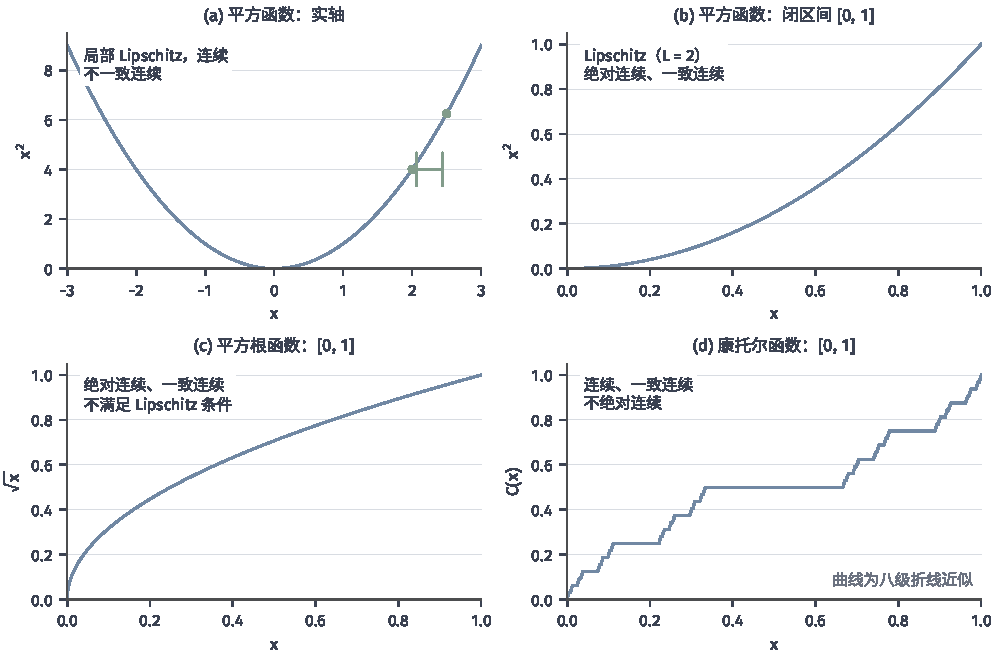
\includegraphics[width=169mm]{figures/01-mathematical-preliminaries-upper/01-mathematical-language-combinatorics-analysis-optimization/matplotlib/continuity-conditions/figure.pdf}
 \caption{连续性条件依赖于函数和定义域。(a)平方函数在实轴上连续且局部Lipschitz，但不一致连续；只展示$[-3,3]$内的曲线，标记对应$x_2=2$、$y_2=2+1/2$，完整反例使用前文的两列输入。(b)同一函数限制到$[0,1]$后为Lipschitz函数，因而绝对连续且一致连续。(c)$\sqrt x$在$[0,1]$上绝对连续、一致连续，却不是Lipschitz函数。(d)康托尔函数在$[0,1]$上连续且一致连续，但不绝对连续。右下曲线为八级折线近似，性质标注属于极限函数；每条有限折线本身都是Lipschitz函数，图形不能代替不绝对连续的证明。}
 \label{fig:analysis-continuity-conditions}
\end{figure*}

\subsubsection{闭区间上连续函数的性质}

\paragraph{有界性与最值}
第~\ref{chap:sets-functions-and-proofs}章的例子说明，函数的下确界未必取得，例如$x$在$(0,1)$上没有最小值。
寻找最小值之前，我们希望知道在什么条件下最值一定存在。
闭区间$[a,b]$中的每个序列都有收敛到区间内某点的子列：Bolzano--Weierstrass定理~\ref{thm:analysis-bounded-subsequence}给出收敛子列，
闭集的序列判据（引理~\ref{lem:analysis-closed-sequence-criterion}）保证极限仍在区间内。
结合连续性，这一事实保证函数有界并达到最值。
\begin{theorem}[闭有界集上的极值定理]
\label{thm:analysis-extreme-value}
设$K\subseteq\mathbb R$非空、闭且有界，$f:K\to\mathbb R$连续，则$f$有界，且在$K$上达到最小值和最大值。特别地，结论适用于非空闭区间。
\end{theorem}
\begin{proof}
若$f$无界，可选$x_n\in K$使$|f(x_n)|>n$。有界序列有收敛子列$x_{n_k}\to x$，闭性保证$x\in K$；连续性给出$f(x_{n_k})\to f(x)$，与$|f(x_{n_k})|>n_k$矛盾。令$m=\inf_K f$，对每个$n$选$x_n\in K$使$m\leq f(x_n)<m+1/n$。再取收敛子列$x_{n_k}\to x^\star\in K$，得到$f(x^\star)=m$。对$-f$重复论证即得最大值。
\end{proof}
\begin{example}[极值定理的条件]
\label{ex:analysis-extrema-failures}
在$(0,1)$上，连续函数$f(x)=x$的下确界为$0$却不达到，因为定义域不含边界点$0$。在闭但无界的实轴上，$e^x$也有未达到的下确界$0$。若在$[0,1]$上令$f(0)=1$、$f(x)=x$（$x>0$），定义域闭且有界，但函数不连续，同样没有最小值。
\end{example}

\paragraph{介值定理}
闭区间上的连续性还保证：函数从一个端点值变化到另一个端点值时，不会遗漏它们之间的数值。
这一结论要求两端之间的整段都在定义域中，条件比前面只要求闭且有界更具体。
\begin{theorem}[介值定理]
\label{thm:analysis-intermediate-value}
设$a,b\in\mathbb R$、$a<b$，$f:[a,b]\to\mathbb R$连续。则
\[
 \begin{gathered}
 \forall c\in[\min\{f(a),f(b)\},\max\{f(a),f(b)\}],\\
 \exists\xi\in[a,b],\quad f(\xi)=c.
 \end{gathered}
\]
若$\min\{f(a),f(b)\}<c<\max\{f(a),f(b)\}$，则可取$\xi\in(a,b)$。
\end{theorem}
\begin{proof}
$c=f(a)$或$c=f(b)$时，直接取相应端点。先设$f(a)<c<f(b)$，令
$S=\{x\in[a,b]:f(x)\leq c\}$。因$a\in S$且$S$有上界$b$，实数的确界性质给出$u=\sup S\in[a,b]$。
对每个正整数$n$，可选$x_n\in S$满足$u-1/n<x_n\leq u$，于是$x_n\to u$。
连续性使$f(x_n)\to f(u)$；由$f(x_n)\leq c$得到$f(u)\leq c$。
这也说明$u\neq b$，因为$f(b)>c$。
若$f(u)<c$，连续性保证$u$右侧充分近的点仍有函数值小于$c$；
由于$u<b$，可在$[a,b]$内选到这样的$v>u$。于是$v\in S$，与$u$为上界矛盾。
因此$f(u)=c$。又因$f(a)<c$，有$u\neq a$，所以$u\in(a,b)$。
若$f(a)>c>f(b)$，对$-f$与$-c$应用同一论证即可。
\end{proof}
介值性使用了整个区间都属于定义域。在$[-2,-1]\cup[1,2]$上，左段恒为$0$、右段恒为$1$的函数连续，却不取中间值$1/2$。
闭且有界足以保证最值，不能代替介值定理中的区间条件。

\paragraph{一般度量空间中的对应结论}
定义~\ref{def:analysis-compactness}已用开覆盖与有限子覆盖规定紧致性；上面的极值证明与一致连续证明，
实际使用的是每个序列都能取到收敛于集合内部的子列。
把同一论证从实轴搬到一般度量空间，需要先在距离语言下证明紧致与序列紧致等价、连续像紧致及紧集上的一致连续；
这些结论在第~\ref{chap:metric-spaces}章完整给出。这里的一元闭有界集满足所需的序列条件，
介值结论则另外依赖定义域是区间，不能由紧致性单独推出。

\par\Needspace{10\baselineskip}
\subsection{微分的定义}
\label{sec:analysis-derivatives-linear-approximation}

连续性描述输入接近时函数值是否接近，还没有记录变化的快慢。下面先用差商的极限定义导数，再把它改写为函数增量的一阶线性近似，由此定义微分。

\subsubsection{导数}

\paragraph{差商}
设$f$在$a$的某个开区间内有定义。输入从$a$变成$a+h$时，函数增量为$\Delta f=f(a+h)-f(a)$。当$h\neq0$，比值$\Delta f/h$称为差商，表示这两个输入之间的平均变化率；在图形上，它是连接两点的割线斜率。

\paragraph{导数}
若差商在$h\to0$时趋于一个有限实数，就定义
\[
 f'(a)=\lim_{h\to0}\frac{f(a+h)-f(a)}h,
\]
称其为$f$在$a$处的\term{导数}（derivative），并称$f$在$a$处可导。导数给出该点的瞬时变化率，也是图形在该点的切线斜率。若区间内每点都可导，则$a\mapsto f'(a)$又构成一个函数，称为导函数。例如$f(x)=x^2$时，差商为$2a+h$，故$f'(a)=2a$。

\paragraph{单侧导数}
在区间端点或尖点附近，左右两侧的变化需要分别观察。
只从$h>0$或$h<0$取极限，分别得到右导数$f'_+(a)$和左导数$f'_-(a)$。内点处的双侧导数存在，当且仅当左右导数都存在、有限并且相等。在闭区间端点讨论导数时，将明确采用从区间内部取得的单侧导数。本节未特别说明的内点导数均指有限的双侧导数。

\subsubsection{可微函数}

\paragraph{可微与微分}

差商趋于$f'(a)$等价于把增量写为
\begin{equation}
 f(a+h)=f(a)+f'(a)h+o(|h|),\qquad h\to0.
\label{eq:analysis-scalar-first-order}
\end{equation}
其中$o(|h|)$表示余项除以$|h|$趋于零，沿用第~\ref{sec:comb-growth-scales}节的记号。

更一般地，若存在实数$A$使$f(a+h)-f(a)=Ah+o(|h|)$，就称$f$在$a$处\term{可微}（differentiable）。除以$h$可见$A$必为$f'(a)$，因此一元实函数在内点可导与可微等价。

一阶近似不仅给出斜率系数，还把输入增量转换为预测的函数增量。
线性映射$h\mapsto f'(a)h$称为$f$在$a$处的\term{微分}（differential），记为$\mathrm df_a(h)$。导数$f'(a)$是实数系数，微分则把输入增量映成预测的函数增量。常用记号$\mathrm df=f'(x)\,\mathrm dx$表达同一关系；有限增量$\Delta f$通常还包含余项，并不等于微分。

例如$x^2$在$a=3$处的导数为$6$。当$h=0.1$时，微分给出$0.6$，实际增量为$3.1^2-3^2=0.61$，两者相差$h^2=0.01$。对$f(x)=x^3-3x$、$a=1/2$，函数值为$-11/8$，导数为$-9/4$，故线性近似为
\begin{equation}
 T_1(h)=-\frac{11}{8}-\frac94h.
\label{eq:analysis-cubic-linear-model}
\end{equation}
取$h=0.1$时，$T_1=-1.600$而$f(0.6)=-1.584$；后面将用二阶导数解释余下的$0.016$。

若$f$在$a$处可微，式~\eqref{eq:analysis-scalar-first-order}右侧的增量趋于零，所以$f$在$a$处连续。

但连续只是可微的必要条件。对$f(x)=|x|$，原点两侧的差商分别为$-1$和$1$，左右导数不相等，因此函数连续却不可微。阶跃函数在原点连连续性都不满足，也就不可微。图~\ref{fig:analysis-continuity-counterexamples}比较了连续可微、连续不可微与不连续三种情形。
\begin{figure*}[htbp]
 \centering
 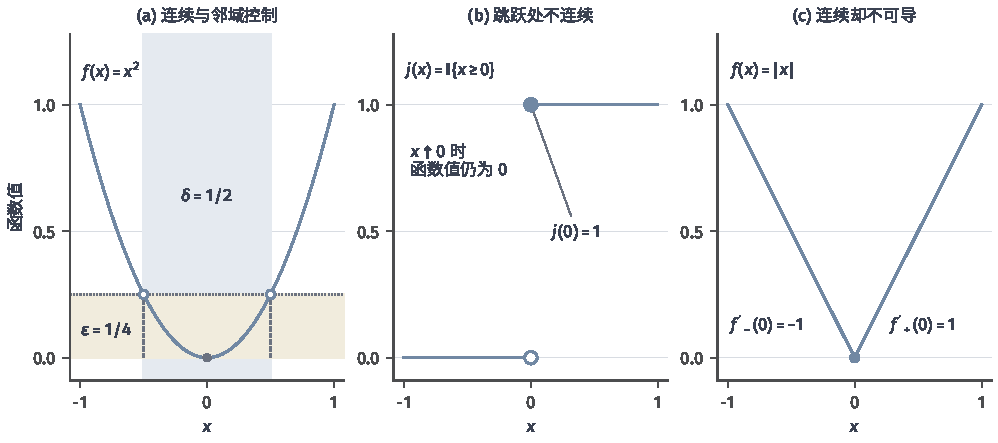
\includegraphics[width=169.0mm]{figures/01-mathematical-preliminaries-upper/01-mathematical-language-combinatorics-analysis-optimization/matplotlib/analysis-continuity-counterexamples/figure.pdf}
 \caption{平方函数、绝对值函数与阶跃函数在原点的差别。平方函数连续且可微；绝对值函数连续，但左右导数不同；阶跃函数的左右极限不同。连续性控制函数值的极限，可微性还要求差商具有同一个有限极限。}
 \label{fig:analysis-continuity-counterexamples}
\end{figure*}

\subsubsection{连续可微函数}

可导以后，还可以要求导函数连续。若$f$在开区间$I$上可导且$f'$连续，称$f$连续可微，记为$f\in C^1(I)$。在闭区间上使用$C^1([a,b])$时，要求$f$在闭区间连续、内点可导，且$f'$连续延拓到两端；延拓值就是相应单侧导数。

连续可微是比可微更强的要求。令$f(0)=0$、$f(x)=x^2\sin(1/x)$（$x\neq0$）。原点差商为$h\sin(1/h)\to0$，所以$f'(0)=0$；非零位置的导数为$2x\sin(1/x)-\cos(1/x)$，将在求导规则中得到。取$x_n=1/(2\pi n)$，有$f'(x_n)=-1$，故$f'$在$0$处不连续。导数存在并没有要求邻近位置的导数也接近它。

\subsection{微分的运算法则}
\label{sec:analysis-scalar-chain-rules}

以下设$f,g$在所讨论点的开邻域有定义，并在该点可导。求导规则来自差商极限或式~\eqref{eq:analysis-scalar-first-order}的一阶展开。

\subsubsection{四则运算的求导}

\paragraph{和与数乘}
差商的加法与数乘直接给出$(f+g)'=f'+g'$、$(cf)'=cf'$，其中$c$为实常数。减法是$c=-1$的情形。

\paragraph{乘积法则}
将$f(a+h)$和$g(a+h)$分别展开，乘积中一次项为$f'(a)g(a)h+f(a)g'(a)h$，两个增量的乘积属于$O(h^2)$。因此
\begin{equation}
 \begin{aligned}
 (f+g)'(a)&=f'(a)+g'(a),\\
 (fg)'(a)&=f'(a)g(a)+f(a)g'(a).
 \end{aligned}
\label{eq:analysis-scalar-sum-product-rules}
\end{equation}

\paragraph{商法则}
若$g(a)\neq0$，连续性先保证$a$附近的分母不为零。整理差商得
\[
 \left(\frac fg\right)'(a)
 =\frac{f'(a)g(a)-f(a)g'(a)}{g(a)^2}.
\]
分母非零既保证函数有定义，也保证右侧公式有意义。

\subsubsection{复合函数求导}

复合函数的输入变化先经过内层，再传入外层；总的一阶变化需要联系这两个局部变化率。
若$f$在$a$处可导，$g$在$f(a)$处可导，且复合在$a$附近有定义，则
\begin{equation}
 (g\circ f)'(a)=g'(f(a))f'(a).
\label{eq:analysis-scalar-chain-rule}
\end{equation}
这称为\term{链式法则}（chain rule）。令$k=f(a+h)-f(a)=f'(a)h+o(|h|)$，则$k=O(|h|)$。把它代入$g(f(a)+k)=g(f(a))+g'(f(a))k+o(|k|)$，余项仍为$o(|h|)$，于是得到公式。$k=0$时取余项为零，这个证明也覆盖$f'(a)=0$的情形，无需除以可能为零的中间增量。

\subsubsection{反函数求导}
逆映射已经连续，现在进一步判断它何时可导，以及变化率怎样由原函数的变化率决定。
设$f:I\to J$在区间$I$上连续且严格单调，$J=f(I)$，其反函数为$g=f^{-1}$。第~\ref{sec:analysis-inverse-continuity}节已证明$g$连续，因此像点趋近时，反像也趋近。若$f$在内点$a$处可导且$f'(a)\neq0$，令$b=f(a)$、$h=g(b+k)-a$，则$k\to0$时$h\to0$，并且
\[
 \frac{g(b+k)-g(b)}k
 =\frac{h}{f(a+h)-f(a)}\longrightarrow\frac1{f'(a)}.
\]
因此$g'(b)=1/f'(a)$。这个公式也与复合恒等式$f(g(y))=y$的链式法则一致；先用差商证明$g$可导，避免在证明中预设它的可导性。条件是所用反函数区间内一一对应，且所讨论点的原函数导数非零。

\paragraph{微分形式的运算法则}
把导数系数作用于增量$h$，同一规则可以写成微分形式：
\[
 \begin{aligned}
 \mathrm d(fg)_a(h)&=g(a)\,\mathrm df_a(h)+f(a)\,\mathrm dg_a(h),\\
 \mathrm d(g\circ f)_a(h)&=\mathrm dg_{f(a)}\bigl(\mathrm df_a(h)\bigr).
 \end{aligned}
\]
复合式先计算中间增量的一阶近似，再把它代入外层微分。

\subsubsection{基本初等函数的导数}
\label{sec:analysis-elementary-derivatives}

四则运算和链式法则把复杂函数的求导归结为基本函数的导数。下面从差商说明常用公式的依据，并给出各自的定义域。

\paragraph{常数函数与整数幂函数}
常数函数$f(x)=c$的差商恒为零，所以$f'=0$；恒等函数$f(x)=x$的差商恒为$1$，所以$f'=1$。
对正整数$m$，把$x^m$看成$m$个恒等函数的乘积，反复使用乘法求导规则。
每一项只对一个因子求导，其余$m-1$个因子保留，于是
\[
 (x^m)'=\underbrace{x^{m-1}+\cdots+x^{m-1}}_{m\text{项}}=mx^{m-1}.
\]
$m=1$时导数为$1$；$m=0$即常数函数。
结合商法则，对负整数$m$在$x\neq0$处同样有$(x^m)'=mx^{m-1}$；正整数幂在整个实轴上使用这一公式。

\paragraph{正弦函数与余弦函数}
采用弧度制。由第~\ref{sec:analysis-function-limits}节的标准极限$\sin h/h\to1$，以及$\cos h-1=-2\sin^2(h/2)$，可得$(\cos h-1)/h\to0$。正弦加法公式于是给出
\[
 \frac{\sin(x+h)-\sin x}{h}
 =\sin x\frac{\cos h-1}{h}+\cos x\frac{\sin h}{h}
 \longrightarrow\cos x.
\]
余弦加法公式同理给出$(\cos x)'=-\sin x$。这两条导数公式在整个实轴成立；若使用角度制，公式还会多出单位换算系数。

\paragraph{指数函数}
自然指数函数满足$e^{x+h}=e^xe^h$。利用前面陈述的标准极限$(e^h-1)/h\to1$，得到
\[
 \frac{e^{x+h}-e^x}{h}=e^x\frac{e^h-1}{h}\longrightarrow e^x.
\]
因此$(e^x)'=e^x$在整个实轴成立。这一推导只使用指数乘法公式与该标准极限。

\paragraph{对数函数与实数幂函数}
前面已知$e^x$连续、严格递增，两端分别趋于$0$与$+\infty$。对任意$y>0$，先选两点使指数值分别小于和大于$y$，再用介值定理得到原像；严格递增保证该原像唯一。因此指数函数的值域恰为$(0,\infty)$，并有反函数。自然对数$\log x$（也记$\ln x$）就定义为这个反函数。指数导数处处非零，反函数求导给出$(\log x)'=1/x$，范围为$x>0$。若$a>0$且$a\neq1$，由$a^x=e^{x\log a}$和$\log_a x=(\log x)/(\log a)$，再用链式法则得到
\[
 (a^x)'=a^x\log a\quad(x\in\mathbb R),\qquad
 (\log_a x)'=\frac1{x\log a}\quad(x>0).
\]
对任意实数$\alpha$，在$x>0$上定义$x^\alpha=e^{\alpha\log x}$，同样得到$(x^\alpha)'=\alpha x^{\alpha-1}$。这并未对负数底数的任意实数次幂作定义。

\subsection{闭区间上可微函数的性质}

导数记录一点处的变化率；现在要把它与区间上的极值、端点变化以及两点之间的变化幅度联系起来。
涉及闭区间$[a,b]$的中值结论将分别要求函数在闭区间上连续、在开区间$(a,b)$内可导，不要求端点具有双侧导数。

\subsubsection{局部极值与驻点}

\paragraph{局部极值}
若只关心某个输入附近的变化，就应先把邻近范围的极值与整个定义域的最值分开。
若存在$r>0$，使定义域内所有满足$|x-c|<r$的点都有$f(x)\geq f(c)$，则$c$称为局部极小点；若$x\neq c$时均为严格不等式，则称为严格局部极小点。
反向不等式定义局部极大点。局部极值只比较某个邻域内的函数值，区别于整个定义域上的最值。

\paragraph{Fermat定理}
局部极值比较邻近函数值，导数则描述一阶变化；两侧差商的符号把这两种信息联系起来。
内点允许从两侧比较，下面说明这种比较对导数的约束。
\begin{theorem}[Fermat定理]
\label{thm:analysis-fermat}
设$a<b$，$f:[a,b]\to\mathbb R$，$c\in(a,b)$。若$f$在$c$处可导，且$c$为$f$的局部极小点或局部极大点，则
\begin{equation}
 f'(c)=0.
\label{eq:analysis-scalar-first-order-necessary}
\end{equation}
\end{theorem}
\begin{proof}
设$c$为局部极小点。充分小的$h$满足$f(c+h)-f(c)\geq0$，
故$h>0$时差商非负、$h<0$时差商非正。
两侧差商趋于同一个有限导数，因而同时有$f'(c)\geq0$与$f'(c)\leq0$，即$f'(c)=0$。
局部极大点对$-f$应用同一论证即可。
\end{proof}
导数为零的点称为\term{驻点}（stationary point），但驻点未必是极值点，例如$x^3$在$0$处。
边界极值也不要求导数为零：$x$在$[0,1]$的最小点为$0$，右导数却为$1$；这里缺少Fermat定理要求的内点条件。

\paragraph{一阶导数判别法}
驻点条件本身不能判定极值，还需考察函数在驻点两侧的变化方向。
下面先给出符号判据，其依据将在后面的单调性小节中证明。
\begin{theorem}[一阶导数判别法]
\label{thm:analysis-first-derivative-test}
设$r>0$，$f$在$[c-r,c+r]$上连续、在$(c-r,c+r)$内可导，且$f'(c)=0$。
若
\[
 f'(x)<0\quad(c-r<x<c),\qquad
 f'(x)>0\quad(c<x<c+r),
\]
则$c$为$f$的严格局部极小点。
若两个区间上的导数符号分别为正和负，则$c$为$f$的严格局部极大点。
\end{theorem}
第一种符号变化对应先降后升，第二种对应先升后降。
仅有$f'(c)=0$不够；接下来先建立中值定理，再由它证明导数符号确实控制区间内的增减，最后补出这一判别法的证明。

\subsubsection{中值定理}

\paragraph{Rolle定理}
当函数两端取同一值时，整体净变化为零。
下面说明连续、可导条件如何保证内部有一处瞬时变化率也为零。
\begin{theorem}[Rolle定理]
\label{thm:analysis-rolle}
设$a<b$，$f:[a,b]\to\mathbb R$在$[a,b]$上连续、在$(a,b)$内可导。
若$f(a)=f(b)$，则
\[
 \exists c\in(a,b),\qquad f'(c)=0.
\]
\end{theorem}
\begin{proof}
若$f$恒定，任取$c\in(a,b)$即可。
否则存在$x_0\in(a,b)$使$f(x_0)\neq f(a)$。
由闭区间上的极值定理，$f$达到最大值和最小值；若$f(x_0)>f(a)=f(b)$，最大值必在内点达到，
若$f(x_0)<f(a)=f(b)$，最小值必在内点达到。
在所选内点应用Fermat定理，得到导数为零。
\end{proof}

\paragraph{Lagrange中值定理}
两端取值不同时，可以先减去连接两个端点的直线，使剩余函数两端相等。
Rolle定理由此把整段平均变化率与某个内点的瞬时变化率联系起来。
\begin{theorem}[Lagrange中值定理]
\label{thm:analysis-lagrange-mean-value}
设$a<b$，$f:[a,b]\to\mathbb R$在$[a,b]$上连续、在$(a,b)$内可导，则存在$c\in(a,b)$使
\begin{equation}
 f(b)-f(a)=f'(c)(b-a).
\label{eq:analysis-mean-value-theorem}
\end{equation}
等价地，$f'(c)=[f(b)-f(a)]/(b-a)$。
\end{theorem}
\begin{proof}
令
\[
 H(x)=f(x)-f(a)-\frac{f(b)-f(a)}{b-a}(x-a).
\]
$H$在$[a,b]$上连续、在$(a,b)$内可导，并满足$H(a)=H(b)=0$。
Rolle定理给出某个$c\in(a,b)$使
$H'(c)=f'(c)-[f(b)-f(a)]/(b-a)=0$，整理即得结论。
\end{proof}
这就是Lagrange\term{中值定理}（mean value theorem）的含义：区间上的平均变化率等于某个内点的瞬时变化率。
定理不要求导函数连续，只要求函数在每个内点可导。


图~\ref{fig:analysis-process-mean-value-parallel}说明中值定理将两个端点之间的平均变化率，联系到区间内部某一点的瞬时变化率。
\begin{figure}[!htbp]
 \centering
 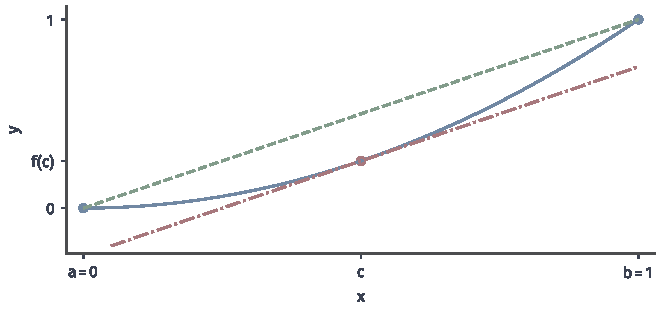
\includegraphics[width=112.0mm]{figures/01-mathematical-preliminaries-upper/01-mathematical-language-combinatorics-analysis-optimization/matplotlib/chapter3-concept-processes/mean-value-parallel.pdf}
 \caption{$f(x)=x^2$在$[0,1]$上，绿虚线为端点割线，红点划线为$c=1/2$处的切线。两线平行，因为$f'(c)=1=[f(1)-f(0)]/(1-0)$。图中切线与割线高度不同；相等的是斜率，而不是两条直线。}
 \label{fig:analysis-process-mean-value-parallel}
\end{figure}

\paragraph{Cauchy中值定理}
同时观察两个函数时，可以把它们的端点增量放进同一个辅助函数，从而联系这两种变化。
采用交叉相乘的形式，可以先得到不依赖分母非零的结论。
\begin{theorem}[Cauchy中值定理]
\label{thm:analysis-cauchy-mean-value}
设$a<b$，$f,g:[a,b]\to\mathbb R$均在$[a,b]$上连续、在$(a,b)$内可导，则存在$c\in(a,b)$使
\[
 (f(b)-f(a))g'(c)=(g(b)-g(a))f'(c).
\]
若进一步有$g'(x)\neq0$对每个$x\in(a,b)$成立，则$g(b)\neq g(a)$，并可写为
\[
 \frac{f(b)-f(a)}{g(b)-g(a)}=\frac{f'(c)}{g'(c)}.
\]
\end{theorem}
\begin{proof}
令
\[
 \begin{aligned}
 H(x)={}&(f(b)-f(a))(g(x)-g(a))\\
        &-(g(b)-g(a))(f(x)-f(a)).
 \end{aligned}
\]
$H$继承两函数的连续、可导条件，并有$H(a)=H(b)=0$。
应用Rolle定理得$H'(c)=0$，展开导数即为交叉相乘形式。
若$g'$处处非零，$g(b)=g(a)$会由Rolle定理推出某个内点$g'=0$，产生矛盾，故端点增量非零。
所选点的$g'(c)$也非零，此时才能除法得到比值形式。
\end{proof}
取$g(x)=x$时，Cauchy中值定理回到Lagrange中值定理。

\subsubsection{单调性}

中值定理把任意两点的函数增量写成一个内点导数乘以输入增量，因此导数符号可以控制整段的增减。
关键是任意两点之间的整段都属于定义域。
\begin{theorem}[导数符号与单调性]
\label{thm:analysis-derivative-monotonicity}
设$a<b$，$f:[a,b]\to\mathbb R$在$[a,b]$上连续、在$(a,b)$内可导。
若$f'(x)\geq0$对所有$x\in(a,b)$成立，则$f$在$[a,b]$上单调不减；若处处有$f'(x)>0$，则严格递增。
相应地，$f'\leq0$蕴含单调不增，$f'<0$蕴含严格递减。
若$f'$在$(a,b)$内恒为零，则$f$在$[a,b]$上为常数。
\end{theorem}
\begin{proof}
任取$a\leq x<y\leq b$，在$[x,y]$上应用Lagrange中值定理，存在$\xi\in(x,y)$使
\[
 f(y)-f(x)=f'(\xi)(y-x).
\]
因为$y-x>0$，右侧的符号由$f'(\xi)$决定，于是得到四种单调性结论。
导数恒为零时，任意两点的函数值都相等，所以函数为常数。
\end{proof}
导数恒零只保证每个区间上为常数。若定义域由分离的区间组成，各段的常数未必相同，不能跨过定义域的缺口使用中值定理。

现在可以补出定理~\ref{thm:analysis-first-derivative-test}的证明：导数的两侧符号分别控制了驻点与任意邻近点之间的变化。
\begin{proof}[一阶导数判别法的证明]
先考虑左负右正的情形。对$c-r<x<c$，在$[x,c]$上应用单调性定理得$f(x)>f(c)$；
对$c<x<c+r$，在$[c,x]$上应用同一定理也得$f(x)>f(c)$。
所以$c$两侧充分近的异点都有更大的函数值，$c$为严格局部极小点。
左正右负时反向比较，得到$f(x)<f(c)$，因此$c$为严格局部极大点。
\end{proof}
导数为零并非严格单调的障碍：例如$x^3$在整个实轴严格递增，但在$0$处导数为零。
因此“导数处处严格为正”是严格递增的充分条件，不能当作必要条件。

\subsubsection{Lipschitz条件}

导数的符号控制增减方向；若还能统一限制导数的绝对值，就可以控制任意两点之间的变化幅度。
中值定理把这一导数上界直接转为前面定义的Lipschitz条件。
\begin{theorem}[有界导数与Lipschitz条件]
\label{thm:analysis-bounded-derivative-lipschitz}
设$a<b$，$f:[a,b]\to\mathbb R$在$[a,b]$上连续、在$(a,b)$内可导。
若存在有限常数$L\geq0$使$|f'(x)|\leq L$对所有$x\in(a,b)$成立，则
\[
 \forall x,y\in[a,b],\qquad |f(y)-f(x)|\leq L|y-x|.
\]
即$f$在$[a,b]$上为Lipschitz连续函数，$L$是一个Lipschitz常数。
\end{theorem}
\begin{proof}
$x=y$时两侧都为零；$x<y$时，Lagrange中值定理给出$\xi\in(x,y)$，使
\[
 |f(y)-f(x)|=|f'(\xi)|\,|y-x|\leq L|y-x|.
\]
$x>y$时交换两点即可。
\end{proof}
例如$f(x)=x^2$在$[0,1]$内有$|f'(x)|=2x\leq2$，所以可以取$L=2$，与前面的直接估计一致。
这一结论仍要求两点间的整段都在定义域中；它给出的是可导函数满足Lipschitz条件的充分保证。

若$f\in C^1([a,b])$，连续导数在闭区间上有界，因而由上述定理得到Lipschitz连续，再由连续性条件的关系得到绝对连续和一致连续。
这些结论的逆向不能保证导数处处存在：$|x|$在$[-1,1]$上Lipschitz连续，却在$0$处不可导。
控制函数值变化与要求经典导数处处存在，因而是两种需要分别检查的条件。

\subsection{高阶微分}

\subsubsection{高阶导数}

\paragraph{二阶导数}
要研究斜率本身怎样变化，可以继续对导函数求导。
导函数$f'$若还可导，其导数称为二阶导数，记为$f''$。

\paragraph{高阶导数}
依次定义$f^{(r)}=(f^{(r-1)})'$，并约定$f^{(0)}=f$。
若直到第$r$阶导数都存在且连续，称$f$为$r$阶连续可微函数，记为$f\in C^r$。$C^r([a,b])$的端点导数采用从内部取得的连续延拓，与前面$C^1$的约定相同。

在以$x$为独立变量的记号中，$r$阶微分写作$\mathrm d^rf=f^{(r)}(x)(\mathrm dx)^r$；它给出高阶变化的系数，近似实际增量时还需Taylor系数与余项。

\subsubsection{二阶近似}
\label{sec:analysis-second-order-curvature}
对$f(x)=x^3-3x$，$f''(x)=6x$，所以$f''(1/2)=3$。加入二次项后，式~\eqref{eq:analysis-cubic-linear-model}成为
\begin{equation}
 T_2(h)=-\frac{11}{8}-\frac94h+\frac32h^2.
\label{eq:analysis-cubic-quadratic-model}
\end{equation}
$h=0.1$时，$T_2=-1.585$，与实际值$-1.584$相差$0.001$。正的二阶导数说明斜率随$x$增加，曲线在这一邻域内向上弯；二次项正好补充切线近似遗漏的这一部分变化。图~\ref{fig:analysis-derivative-orders}比较了两阶近似及其余项。

\subsubsection{Taylor公式}
\label{sec:analysis-taylor-approximation}

\paragraph{Lagrange余项}
要把上面的近似推广到任意阶，需要同时控制截去的误差。设$r\geq0$为整数，$f$在连接$x_0$与$x_0+h$的线段的开邻域内属于$C^{r+1}$。若$h\neq0$，则两端之间存在$\xi$使
\begin{equation}
 f(x_0+h)=\sum_{k=0}^r\frac{f^{(k)}(x_0)}{k!}h^k
 +\frac{f^{(r+1)}(\xi)}{(r+1)!}h^{r+1}.
\label{eq:analysis-taylor-arbitrary-order}
\end{equation}
\begin{proof}
记$T_r(t)=\sum_{k=0}^rf^{(k)}(x_0)(t-x_0)^k/k!$，$R=f(x_0+h)-T_r(x_0+h)$。令
\[
 H(t)=f(t)-T_r(t)-R\frac{(t-x_0)^{r+1}}{h^{r+1}}.
\]
$H$在两端为零，且$r\geq1$时$H'(x_0),\ldots,H^{(r)}(x_0)$均为零。第一次用Rolle定理得到两端之间的零导数点，再把该点与$x_0$的零导数条件结合，逐次使用Rolle定理。共用$r+1$次后得到某个中间点$\xi$满足
\[
 0=H^{(r+1)}(\xi)=f^{(r+1)}(\xi)-\frac{(r+1)!}{h^{r+1}}R.
\]
整理即得公式。$r=0$时只用一次Rolle定理；$h<0$时交换区间左右端点，论证相同。
\end{proof}
若该线段上$|f^{(r+1)}|\leq M$，余项的绝对值不超过$M|h|^{r+1}/(r+1)!$。因此近似的精度既与阶数有关，也与位移大小及导数界有关。第~\ref{sec:analysis-integration-remainders}节还将给出积分余项，本处的证明不依赖积分。

对立方函数，完整展开为
\[
 f(1/2+h)=-\frac{11}{8}-\frac94h+\frac32h^2+h^3.
\]
线性近似遗漏$3h^2/2+h^3$，二次近似只遗漏$h^3$；四阶及以上导数全为零，三阶展开已经精确。
\begin{figure*}[htbp]
 \centering
 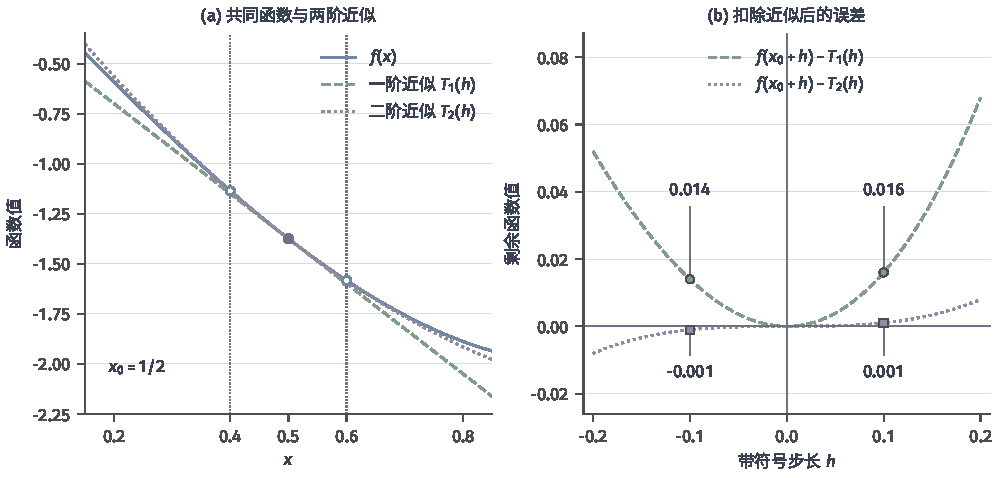
\includegraphics[width=169.0mm]{figures/01-mathematical-preliminaries-upper/01-mathematical-language-combinatorics-analysis-optimization/matplotlib/analysis-derivative-orders/figure.pdf}
 \caption{$f(x)=x^3-3x$在$x_0=1/2$处的Taylor近似，$h=x-x_0$。左图比较原函数、切线近似$T_1$与二次近似$T_2$；右图给出相应的带符号余项$3h^2/2+h^3$和$h^3$。标记点对应$h=\pm0.1$，余项的正负说明真值位于近似值的哪一侧。}
 \label{fig:analysis-derivative-orders}
\end{figure*}

\paragraph{Peano余项}
如果只关心位移趋零时的误差阶，可以不保留中间点，改用小量记号描述余项。
若$f\in C^r$、$r\geq1$，则在$x_0$附近有
\[
 f(x_0+h)=\sum_{k=0}^r\frac{f^{(k)}(x_0)}{k!}h^k+o(|h|^r).
\]
对$r-1$次Taylor公式使用Lagrange余项，再从$f^{(r)}(\xi_h)h^r/r!$中减去$f^{(r)}(x_0)h^r/r!$。因为$\xi_h\to x_0$且$f^{(r)}$连续，差除以$|h|^r$趋零，就得到这一形式。它描述局部误差的阶；若需要有限位移下的具体界，可使用上面的Lagrange余项估计。

\paragraph{二阶导数判别法}
在驻点处，一阶项为零；二阶Taylor公式把局部增减进一步联系到二阶导数的符号。
设$f$在驻点$a$附近属于$C^2$。Taylor公式给出$f(a+h)-f(a)=\tfrac12f''(\xi_h)h^2$。若$f''(a)>0$，连续性使充分近的$f''(\xi_h)\geq f''(a)/2$，因而非零小增量使函数值严格增加，$a$为严格局部极小点；$f''(a)<0$时为严格局部极大点。反之，在上述$C^2$条件下，局部极小点必须有$f''(a)\geq0$，局部极大点必须有$f''(a)\leq0$。

$f''(a)=0$时该判别法没有结论：$x^4$、$-x^4$在$0$处分别有严格局部极小值和极大值，$x^3$则没有极值，三者在原点的前两阶导数都为零。

\FloatBarrier

\section{集合的测量}
\label{sec:comb-set-measurement}
\label{sec:analysis-set-structures}

区间$[a,b]$的长度是$b-a$，但实轴上的集合未必是一个区间。
本节要解决的问题是：怎样把区间的长度推广到更一般的实数集合，并在原来的区间上仍得到$b-a$？
这样的长度概念将用于后面的积分：将输入范围分成若干块后，需要知道各块的大小，才能按这些大小累计函数取值。
有限集合的元素个数与加权计数提供另一类测量例子，可以先用它们说明为集合赋予大小时应遵守的相加规则。

距离与大小是两种不同的结构。同一个实轴及其通常距离，既可以测量区间长度，也可以计算集合中的点数；
因此，选定度量并没有唯一确定测度。

本节先用有限集合的计数与加权计数说明相加规则，再从区间长度构造Jordan测量，
并用有理点集说明有限覆盖的局限；随后引入可数集，用可数覆盖定义勒贝格外测度；
再通过精确分割条件选出可测集，在可测集上得到可数可加的勒贝格测度；
最后把这些性质抽象为一般测度空间，研究集合列的测度、零测集与集合的逼近。

\subsection{有限集与Jordan测量}
\label{sec:comb-counting-to-weight}

我们先把目标限制在有界的实数集合上，希望给这些集合建立与区间长度相容的测量方法。
例如$[0,1]\cup[2,3]$由两段互不重叠、长度各为$1$的区间组成，总长度应为$2$。
这说明所求的测量应满足一条规则：集合分成有限个两两不交的部分时，总量等于各部分测量值之和。

下面先在有限集合上用计数和加权计数说明这条规则，再回到实轴。
实轴上的长度将从区间出发，先计算有限个区间的并，再用这些简单集合逼近更一般的有界集合；
只有当内部与外部的长度估计能逼近同一个数时，才用这个数定义集合的Jordan测量。

\subsubsection{有限集的测量}

\paragraph{计数与加权计数}

在有限集合上，最直接的测量是数元素个数；若不同元素代表不同的份量，还可以给每个元素指定权重。
设$X=\{x_1,\ldots,x_m\}$中的点互异，每点带有非负权重$w_i$。
把落在$A\subseteq X$中的点的权重相加，定义
\[
 \mu(A)=\sum_{i:x_i\in A}w_i.
\]
所有$w_i=1$时，$\mu(A)=|A|$；改变权重时，元素不变，测量值却可以改变。
例如$X=\{a,b\}$，给$a,b$的权重分别为$1,2$，就有
$\mu(\{a\})=1$、$\mu(\{b\})=2$、$\mu(X)=3$。

若$A_1,\ldots,A_k$两两不交，每个点只落入其中一组，故
\[
 \mu\left(\bigcup_{j=1}^k A_j\right)=\sum_{j=1}^k\mu(A_j).
\]
这称为\term{有限可加性}（finite additivity）。它沿用计数的加法规则，
但相加的是各组的权重，不必是元素个数。

\paragraph{集合权重与函数值}

前面的$\mu(A)$只测量集合$A$本身。后面还要在集合上累计函数取值，届时每个点的贡献等于函数值乘以该点的权重。
例如固定前面的$X=\{a,b\}$，若$f(a)=3,f(b)=-1$，
不加权的取值和为$3-1=2$；按上述权重求和则为$3\cdot1+(-1)\cdot2=1$。
两种规则下的集合权重分别为$2$与$3$，函数的取值和则分别为$2$与$1$。
表~\ref{tab:analysis-metric-measure-integral}列出这些计算；后面的积分将把这种加权累计扩展到更一般的函数。
\begin{table}[htbp]
 \centering\small
 \begin{tabularx}{\linewidth}{@{}lXX@{}}
 \toprule
 考察对象 & 所用规则 & $X=\{a,b\}$上的结果\\
 \midrule
 元素个数 & 每点计$1$ & $|X|=2$\\
 集合权重 & $a,b$分别计$1,2$ & $\mu(X)=3$\\
 数值的等权累计 & 取值为$3,-1$ & $3-1=2$\\
 数值的加权累计 & 同一取值采用权重$1,2$ & $3-2=1$\\
 \bottomrule
 \end{tabularx}
 \caption{有限计数与加权累计。相同的元素范围和相同的数值取值仍可采用不同权重；只有先固定权重，累计值才有确定含义。}
 \label{tab:analysis-metric-measure-integral}
\end{table}

\paragraph{点数与长度}

有限集合的例子说明了不交部分如何相加，但每点计$1$的规则不能给出区间长度。
例如$[0,1]$和$[0,2]$都含有无限多个点，逐点计数都得到无穷，而它们的长度分别应为$1$和$2$。
所以，要推广区间长度，必须另行规定与几何长度相容的测量规则。

单点$[a,a]$的长度为$0$，有限个单点的并也应有长度$0$。这与非退化区间长度为正并不矛盾：区间不能写成有限个单点的并，有限可加性并不适用于将它拆成全部单点的操作。后面还会说明，非退化区间也不能按可数个单点列举。

我们下面以区间长度为起点，先给能由有限个区间组成的集合计算长度，再研究不能这样表示的集合。

\subsubsection{Jordan测量}

\paragraph{区间长度与初等集}

一个区间的长度由端点决定；有限个区间组成的集合，也可以先拆成互不重叠的小段再相加。

为反复使用这类可以直接计算长度的集合，先给它们一个名称。
对端点为$a\leq b$的有界区间$I$，规定长度为$\ell(I)=b-a$，不因端点是否包含而改变；
单点与空集的长度为$0$。

我们把有限个这样的区间的并称为\term{初等集}（elementary set），空集也约定为初等集。
例如$[0,1]\cup[2,3]$是初等集，可以将两段长度相加得到$2$。
区间发生重叠时，需要先消除重复计算：$[0,2]\cup[1,3]=[0,3]$的长度为$3$，不能把原来两段的长度直接相加为$4$。

一个初等集可以有多种区间表示。将所有端点排序后，按相邻端点间的开区间及端点本身切分，得到有限个两两不交的小段；只对属于该集合的小段长度求和，记为$\ell(B)$。
若采用另一种表示，把两组端点一起排序，便得到共同的细分；
区间从$c$处分成两段时，$(c-a)+(b-c)=b-a$，所以细分不改变总长度。
因此，$\ell(B)$不依赖原来的表示。

由同一细分可知，初等集的并、交、差仍为初等集；
不交初等集的长度有限可加。一般有限覆盖则只给出不等式：
若$B\subseteq\bigcup_{j=1}^k B_j$，有
$\ell(B)\leq\sum_{j=1}^k\ell(B_j)$，因为重叠小段可能在右侧被重复计算。

\paragraph{内容量与外容量}

初等集的长度已经可以计算，但有界集合只要求一个集合包含在某个有限区间内，并不要求它本身由有限个区间组成。
例如
\[
 E=\{1,1/2,1/3,\ldots\}\subseteq[0,1]
\]
就是一个有界集合，但它不是由有限个区间组成的初等集。

对任意$u>0$，$E\cap[u,1]$中的点$1/n$都满足$n\leq1/u$，所以这一部分只有有限多个点。
因此$E$不包含任何正长度区间：假如包含，就能从中截取一段左端点大于$0$的正长度区间，与刚才的有限性矛盾。若用有限个区间恰好拼出$E$，这些区间就只能退化成单点；有限个单点又不能组成$E$中的无限多个点。
所以前面针对初等集的长度公式尚不能直接用于$E$。

为了能对$E$这样的集合进行测量，一种办法是保留初等集作为计算工具，用包含关系给出长度估计。
把初等集$A$放在$E$内部，即$A\subseteq E$，$\ell(A)$就应是$E$长度的下界；
用初等集$B$包住$E$，即$E\subseteq B$，$\ell(B)$就应是上界。
我们希望内部估计尽可能大、外部估计尽可能小，因此分别取内部长度的上确界与外部长度的下确界。
这两个数未必相等；但如果相等的话，我们就可以用内部与外部的估计才共同确定一个长度值，以此来作为对$E$的测量。

我们下面将这两个界分别记下来，并以它们是否相等规定哪些有界集合可以用这种方法测量。
这里的候选都是有限区间并，所用的长度$\ell$已经在前面定义。
\begin{definition}[Jordan内容量与外容量]
\label{def:analysis-jordan-content}
对有界集合$E\subseteq\mathbb R$，定义\term{Jordan内容量}（Jordan inner content）与\term{Jordan外容量}（Jordan outer content）为
\[
 \begin{aligned}
 j_*(E)&=\sup\{\ell(A):A\subseteq E,\ A\text{为初等集}\},\\
 j^*(E)&=\inf\{\ell(B):E\subseteq B,\ B\text{为初等集}\}.
 \end{aligned}
\]
若$j_*(E)=j^*(E)$，称$E$为Jordan可测集，二者的共同值记为$j(E)$，称为它的\term{Jordan测量}（Jordan measure）值。
\end{definition}

有界性保证外部候选非空且长度有限；空集是内部候选，所以
$0\leq j_*(E)\leq j^*(E)<\infty$。
上下确界不要求由某个最佳初等集取得。
例如$E$本身是初等集时，内外都可选$E$，故$j(E)=\ell(E)$。
这保证新的定义保留了原来的区间长度与有限区间并的长度，有限点集的测量值也仍为$0$。

再看刚才的$E=\{1/n:n\geq1\}$。它不含正长度区间，内部初等集只能是有限点集，所以
\[
 j_*(E)=0
\]

对每个整数$N\geq2$，取
\[
 B_N=\{1,1/2,\ldots,1/(N-1)\}\cup[0,1/N].
\]
前$N-1$个点分别由单点覆盖，其余点全部落在$[0,1/N]$内，故$E\subseteq B_N$。
由于$B_N$是初等集，长度为$1/N$，所以$0\leq j^*(E)\leq1/N$对所有$N\geq2$成立，从而
\[
 j^*(E)=0
\]

内外容量相等，说明这个不属于初等集的无限点集仍然Jordan可测，而且$j(E)=0$。
这里的长度值来自有限逼近的误差$1/N$趋于零。

\paragraph{有限逼近与可加性}

内外数值相等也可以改写成误差条件：$E$为Jordan可测集，当且仅当对每个$\varepsilon>0$，
存在初等集$A\subseteq E\subseteq B$，使$\ell(B)-\ell(A)<\varepsilon$。
正向根据上确界和下确界各选一个误差小于$\varepsilon/2$的候选；
反向利用$j_*(E)$与$j^*(E)$始终夹在这两个长度之间。

这个夹逼条件还保证有限次集合运算保持Jordan可测性。
例如分别以$A_E\subseteq E\subseteq B_E$和$A_F\subseteq F\subseteq B_F$夹住两个集合，
它们的并可由$A_E\cup A_F$、$B_E\cup B_F$夹住，
新上下界之间的长度差不超过原来两份误差之和。
交集使用内、外逼近的交；差集使用$A_E\setminus B_F$与$B_E\setminus A_F$，
漏出的部分同样包含于原来的两份误差中。
因此，有限并、交、差均保持可测性。

若$E,F$还不交，内部逼近$A_E,A_F$也不交，于是
\[
 \ell(A_E)+\ell(A_F)
 \leq j_*(E\cup F)\leq j^*(E\cup F)
 \leq\ell(B_E)+\ell(B_F).
\]
让各份逼近误差趋零，得到$j(E\cup F)=j(E)+j(F)$。
这就是Jordan测量的有限可加性；它依赖有限次逼近误差仍能控制，而非任意多次并的封闭性。

\subsubsection{Jordan测量的局限}

\paragraph{有理点集的内外容量}

前面的倒数点集$E$虽然不是初等集，仍能用有限区间并把外部长度压到任意小。
这是否意味着每个有界集合都能这样处理？我们下面考察$Q_0=\mathbb Q\cap[0,1]$，说明Jordan方法使用的有限逼近并不能处理任意的有界集合。

先看$Q_0$在区间中的分布。任意非退化实区间$(a,b)$（$a<b$）都含有有理数和无理数。
先找有理数：取正整数$q>1/(b-a)$，相邻分数$p/q$与$(p+1)/q$的间距$1/q$小于区间长度。
令$p$为满足$p>aq$的最小整数，则$(p-1)/q\leq a<p/q$，于是$p/q\leq a+1/q<b$，即$p/q\in(a,b)$。

再找无理数：对区间内的有理数$r$，取正整数$k$使$\sqrt2/k<b-r$，则$r+\sqrt2/k$位于$(r,b)$内；
它若是有理数，$\sqrt2=k(r+\sqrt2/k-r)$也将是有理数，矛盾。
所以$Q_0$和它在$[0,1]$内的补集都与每一段正长度子区间相交。

内部逼近因此很小：任何正长度区间都含有无理数，不可能完全落在$Q_0$中。
包含于$Q_0$的初等集只能由有限个单点组成，长度为零，所以
\[ 
 j_*(Q_0)=0
\]

外部逼近却受到另一种限制。设初等集$B$包含$Q_0$，把组成$B$的有限个区间的端点补齐，得到闭包$\overline B$；
补上有限个点不改变长度，所以$\ell(\overline B)=\ell(B)$。
若$[0,1]$内某点不在$\overline B$，由于$\overline B$闭，这个点附近就有一小段完全避开$B$。
这段在$[0,1]$内的部分含有有理数，与$Q_0\subseteq B$矛盾。
因此$[0,1]\subseteq\overline B$，从而$\ell(B) = \ell(\overline B) \geq 1$。
又因为$[0,1]$本身就是一个外部候选，得到
\[
 j^*(Q_0)=1.
\]

内部逼近和外部逼近两种估计之间始终相差$1$，所以$Q_0$不Jordan可测。

\paragraph{有限覆盖的限制}

$Q_0$无法Jordan可测的问题不在于区间分得还不够多。无论选一百个还是一百万个区间，只要仍是有限个，它们的并就是初等集，上面的证明仍迫使任何覆盖$Q_0$的总长度至少为$1$。
这与倒数点集的情形不同：倒数点集可以把除有限点以外的全部点装进靠近零的一个短区间，
而有理点集在$[0,1]$的每一小段中都出现，不能用一个越来越短的区间收拢剩下的点。

要突破这个下界，需要扩大允许使用的覆盖，而不是继续增加某一次有限覆盖的区间数。
如果能将$Q_0$列为$q_1,q_2,\ldots$，就可以给每个点分别安排一个开区间，
并把长度依次限制为$\varepsilon/2,\varepsilon/4,\varepsilon/8,\ldots$。
每个点都会被覆盖，而总长度由几何级数控制在$\varepsilon$以内；$\varepsilon$又可以任意小。
这里需要一列区间同时覆盖全部点，任意一个有限前段本身都未必覆盖$Q_0$。
图~\ref{fig:measure-countable-cover}对比了两种覆盖规则；右侧的前四项只展示长度如何分配，并未单独完成对全部有理点的覆盖。

\begin{figure*}[htbp]
 \centering
 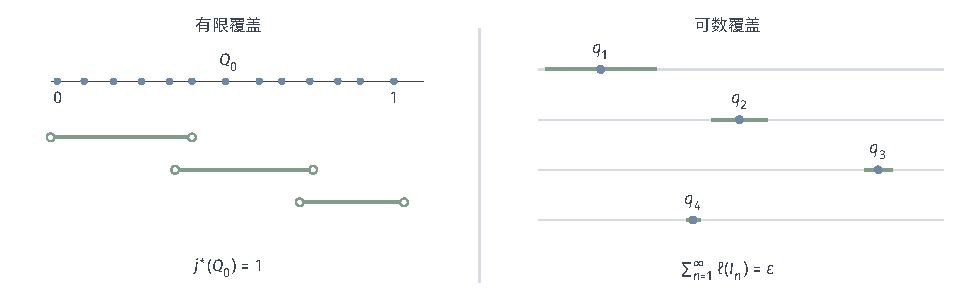
\includegraphics[width=169mm]{figures/01-mathematical-preliminaries-upper/01-mathematical-language-combinatorics-analysis-optimization/tikz/measure-countable-cover/figure.pdf}
 \caption{有限覆盖与可数覆盖。左侧画出一个有限开区间覆盖示例；对$Q_0=\mathbb Q\cap[0,1]$的任意有限区间覆盖，总长度均不小于$1$。右侧将一次完整覆盖改为可数个区间，图中取$\varepsilon=0.8$，只画列举中前四个点及其区间，长度依次为$\varepsilon2^{-n}$；使用全部区间时覆盖全部有理点，总长度为$\varepsilon$，并可随$\varepsilon$任意减小。点的有限示意不能表示有理点的完整稠密分布。}
 \label{fig:measure-countable-cover}
\end{figure*}


这给出新的思路：允许可数个区间组成一次完整覆盖，再用非负级数计算总长度。
第~\ref{sec:comb-countable-sets}节已经建立所需的列举与合并规则。下面先把这些规则用于覆盖，
再检查非负级数的合并，最后定义采用可数覆盖的外部长度估计。

\subsection{可数集与勒贝格外测度}
\label{sec:analysis-countable-outer-measure}

有限覆盖的限制已经给出了改变构造的理由：让每个可列举的点都能分到自己的小区间，
同时把所有区间的总长度控制住。可数覆盖使这两件事能够同时实现，因为区间有自然数编号，长度可以用已经学过的非负级数相加。

为使这一做法适用于后面的推导，先回用可数个可数集合的并仍可数，保证覆盖合并后仍在允许范围内；
非负双重级数可以合并，保证按组或统一编号计算覆盖长度得到同一个总和。
这些工具建立后，就能定义勒贝格外测度，并检查它既能改进有理点集的估计，又保留普通区间的长度。

\subsubsection{可数覆盖的编号与长度}

第~\ref{sec:comb-countable-sets}节已定义可数集，并用对角列举证明自然数对、有理数与可数个可数集的并可数。
因此$Q_0=\mathbb Q\cap[0,1]$可列为$\{q_1,q_2,\ldots\}$，每个点都能分到自己的小区间；
合并一列可数覆盖时，区间也仍可统一编号。
这里还需要检查总长度：改变非负项的列举方式，不能改变覆盖长度的总和。

\paragraph{非负双重级数的合并}

编号解决能否列举，级数规则还要保证改变列举方式不会改变覆盖总长度。
回用前面的非负项级数定义，对$a_n\in[0,\infty]$有
\begin{equation}
 \sum_{n=1}^{\infty}a_n
 =\sup_{N\geq1}\sum_{n=1}^Na_n\in[0,\infty].
 \label{eq:comb-nonnegative-sum-supremum}
\end{equation}
非负性使有限和随加入新项而增加，所以也可对所有有限索引集取上确界，结果相同。

对$a_{n,j}\geq0$，将双指标按任一无遗漏、无重复的顺序列成一个序列，总和便是
\[
 S=\sup_{F\subseteq\mathbb N_+^2,\,F\text{有限}}
          \sum_{(n,j)\in F}a_{n,j}.
\]
这个值等于$\sum_n\sum_j a_{n,j}$，也就是先对每一行求和、再把各行之和相加。下面分两个方向证明。

一个方向：任取有限索引集$F$，它只涉及有限多行，并在每一行中只取有限多项；
每行取出的部分不超过该行之和，所以$\sum_{(n,j)\in F}a_{n,j}\leq\sum_n\sum_ja_{n,j}$，对$F$取上确界得$S\leq\sum_n\sum_ja_{n,j}$。

反方向：固定行数$N$与任意$\varepsilon>0$，若各行之和都有限，对每个$n\leq N$选有限列数$J_n$，
使该行前$J_n$项之和超过整行之和减去$\varepsilon/N$。这些项组成一个有限索引集，所以
$S\geq\sum_{n=1}^N\sum_ja_{n,j}-\varepsilon$。令$\varepsilon\downarrow0$，再对$N$取上确界，得到$S\geq\sum_n\sum_ja_{n,j}$。
若某行之和为无穷，它的有限部分和可以超过任意给定的有限上界，同样迫使$S=+\infty$，两侧都为无穷。

证明只使用有限和与上确界的性质，这就为此处非负项的换序提供了依据，无须调用后文的积分换序定理。

\subsubsection{勒贝格外测度}
\label{sec:comb-length-and-lebesgue-measure}

\paragraph{可数区间覆盖}

前面已经证明$Q_0$可以列为$q_1,q_2,\ldots$，逐点安排小区间的方案因此可以实施。
我们把这种覆盖方式用于一般集合：对$E\subseteq\mathbb R$，选择有限或可数个有界开区间$I_j=(a_j,b_j)$，
只要求$E\subseteq\bigcup_j I_j$，称它们为$E$的可数区间覆盖。
区间可以重叠，也可以伸出$E$；它们的总长度为非负级数$\sum_j(b_j-a_j)$，允许等于$+\infty$。

“可数”限制的是覆盖区间的个数，不是$E$中的点数；一个开区间就可以覆盖含有不可数多个点的闭区间。
选择可数覆盖，是为了能逐项分配误差、用级数累计长度，并在合并覆盖时保留这两种能力。
前面没有给任意不可数族定义总长度，因此这里也不把“可数”直接换成不受限制的任意集合族。
采用开区间还使闭区间的有限子覆盖性质可以参与证明，下面将用它保证原来的区间长度不被改变。

\paragraph{勒贝格外测度的定义}

一次覆盖可能伸出集合，也可能重复覆盖某些位置，总长度只是一个外部估计，依赖于区间的选择。
为了尽量排除这些额外长度，我们对所有允许覆盖的总长度取下确界，得到勒贝格外测度。
\begin{definition}[勒贝格外测度]
\label{def:analysis-lebesgue-outer-measure}
对$E\subseteq\mathbb R$，定义其\term{勒贝格外测度}（Lebesgue outer measure）为
\begin{equation}
 m^*(E)=\inf\left\{\sum_{j=1}^{\infty}(b_j-a_j):
 \begin{array}{l}
 E\subseteq\bigcup_{j=1}^{\infty}(a_j,b_j),\\
 -\infty<a_j<b_j<\infty
 \end{array}\right\}.
 \label{eq:comb-lebesgue-outer-measure}
\end{equation}
这里也允许有限覆盖以及空集的空覆盖；空和为$0$。
\end{definition}

任意集合都能由覆盖整条实轴的一列区间覆盖，所以候选始终非空。
其下确界可为无穷，也不必由某个覆盖达到。
例如单点可以被任意短的开区间覆盖，其外测度为$0$；不存在长度为$0$的非空开区间来达到这个下确界。

\paragraph{空集与单调性}

空覆盖表明$m^*(\varnothing)=0$。
若$E\subseteq F$，任何覆盖$F$的区间族也覆盖$E$，
所以$E$的候选至少与$F$一样多，取下确界便得$m^*(E)\leq m^*(F)$。
这称为外测度的单调性，依据是允许覆盖之间的包含关系。

\paragraph{区间的外测度}

允许可数覆盖后，候选更多，下确界可能下降。我们希望有理点集的估计可以下降，同时必须检查普通区间的长度仍是原值。
先证明$m^*([a,b])=b-a$。上界用$(a-\varepsilon/2,b+\varepsilon/2)$覆盖$[a,b]$，再令$\varepsilon\downarrow0$。
下界必须控制每一种可数覆盖，不能只考察某一组区间。任取可数开区间覆盖，由闭区间的有限子覆盖性质，
其中有限个区间已经覆盖$[a,b]$，所以初等集的有限覆盖不等式给出
\[
 b-a\leq\sum_{j\in F}(b_j-a_j)\leq\sum_{j=1}^{\infty}(b_j-a_j),
\]
其中$F$是选出的有限索引集。对所有可数覆盖取下确界，得到反向界。
因此闭区间外测度等于长度；对任意端点型式的非退化区间$I$，
在它内部放入长度趋向$b-a$的闭区间，再用单调性夹逼，也得到$m^*(I)=b-a$。
无界区间包含任意长的有界闭区间，故其外测度为$+\infty$。

\paragraph{可数点集的外测度}

现在回到推动构造的例子，检验可数覆盖是否真正突破了有限覆盖的限制。
设$E=\{x_1,x_2,\ldots\}$可数，任给$\varepsilon>0$，对每个$n$取
\[
 I_n=\bigl(x_n-\varepsilon2^{-n-1},\ x_n+\varepsilon2^{-n-1}\bigr).
\]
每个点$x_n$都落入$I_n$，所以这列区间覆盖全部$E$，且$\ell(I_n)=\varepsilon2^{-n}$。
这组覆盖满足
\[
 0\leq m^*(E)\leq\sum_{n=1}^{\infty}\varepsilon2^{-n}=\varepsilon.
\]
由于$\varepsilon$任意，得到$m^*(E)=0$，有限集也可同样处理。
这里每个覆盖区间的长度都为正；趋向零的是全部覆盖的总长度上界，而不是在相加一些未定义的正“无穷小”。

特别地，$m^*(Q_0)=0$，尽管它的Jordan外容量为$1$。
有限覆盖的下界为$1$，可数覆盖却能把总长度压到任意给定的正误差以内；改变的是一次完整覆盖所允许的区间族。
这与$m^*([0,1])=1$也不矛盾：$Q_0$可数，能够逐点编号，整个区间却不可数，无法给其中全部点各分配上述自然数编号。

到这里，我们已经得到每个集合的外测度值，还没有证明这些值在不交集合之间能够精确相加。
因此$m^*(Q_0)=0$先回答了外部估计的问题；要把外测度用于稳定的分块累计，还需要下面的可加性与可测性。

\subsubsection{可数可加性}

\paragraph{可数可加性的要求}

新的覆盖方式已经处理了可数次累计，我们也希望测量规则能处理可数次不交分割。
例如，若一个可数点集能作为各个单点的不交并参与精确相加，它的总长度就应由单点长度之和确定。

一般地，对赋值$\nu$，希望有
\[
 \nu\left(\bigcup_{n=1}^{\infty}E_n\right)=\sum_{n=1}^{\infty}\nu(E_n),
 \qquad E_i\cap E_j=\varnothing\ (i\neq j),
\]
其中并集与各部分都应在$\nu$的赋值范围内。
这称为\term{可数可加性}（countable additivity），右侧是已经定义的非负项级数。

区间不可数，因而此要求不允许把一个区间拆成全部单点后当作可数级数求和；
单点外测度为零与区间外测度为正并不矛盾。

\paragraph{外测度的可数次可加性}

先从已经建立的覆盖构造推出一个能够保证的结论：把每个集合的覆盖合并，就得到并集的覆盖，
所以并集的外测度不超过各部分外测度之和。这只是不等式，并且不要求各集合不交。
这项性质称为\term{可数次可加性}（countable subadditivity）；名称中的“次”表示这里保证的是上界，不是精确相等。

每个集合未必有达到外测度的最优覆盖，证明时只能选近似最优覆盖。
因此需要把第$n$组的误差限制为$\varepsilon2^{-n}$，使合并无穷多组后总误差仍不超过$\varepsilon$。
\begin{theorem}[勒贝格外测度的可数次可加性]
\label{thm:analysis-outer-subadditivity}
对任意$E_1,E_2,\ldots\subseteq\mathbb R$，有
\begin{equation}
 m^*\left(\bigcup_{n=1}^{\infty}E_n\right)
 \leq\sum_{n=1}^{\infty}m^*(E_n).
 \label{eq:analysis-outer-subadditivity}
\end{equation}
\end{theorem}
\begin{proof}
若右侧为$+\infty$，不等式直接成立。
设右侧有限，则每个$m^*(E_n)$有限。给定$\varepsilon>0$，由下确界定义，
为每个$E_n$选择覆盖$\{I_{n,j}:j\geq1\}$，使
\[
 E_n\subseteq\bigcup_j I_{n,j},\qquad
 \sum_j\ell(I_{n,j})<m^*(E_n)+\varepsilon2^{-n}.
\]
空集可以取空覆盖，有限覆盖直接作为有限组处理。
所有$I_{n,j}$覆盖$\bigcup_nE_n$；可数个可数集的并仍可数，故它们是允许使用的一组覆盖。
再由非负双重级数的合并规则，
\[
 \begin{aligned}
 m^*\left(\bigcup_nE_n\right)
 &\leq\sum_{n,j}\ell(I_{n,j})\\
 &=\sum_n\sum_j\ell(I_{n,j})
 \leq\sum_nm^*(E_n)+\varepsilon.
 \end{aligned}
\]
最后让$\varepsilon\downarrow0$，得到所需不等式。
\end{proof}

\paragraph{一般外测度}

刚才的证明只给出不等式，尚未要求不交集合的值精确相加。
把已经得到的三条性质抽取出来，便得到可用于其他测量构造的一般概念。
\begin{definition}[外测度]
\label{def:analysis-outer-measure}
集合$X$上的映射$\mu^*:\mathcal P(X)\to[0,\infty]$，若满足
\[
 \begin{gathered}
 \mu^*(\varnothing)=0,\\
 A\subseteq B\Longrightarrow\mu^*(A)\leq\mu^*(B),\\
 \mu^*\left(\bigcup_{n=1}^{\infty}E_n\right)\leq\sum_{n=1}^{\infty}\mu^*(E_n)
 \quad(E_n\subseteq X),
 \end{gathered}
\]
则称为\term{外测度}（outer measure）。
\end{definition}
勒贝格外测度是一个实例。刚才的覆盖合并证明了定义中的第三条性质，却没有给出反向不等式。
即使$E_n$两两不交，分别覆盖它们的开区间也可能彼此重叠；集合不交并不会自动使覆盖的长度精确相加。
反过来，把覆盖并集的区间按任意集合切开，所得部分又未必是区间，不能直接沿用区间长度公式来分配总量。
因此，不能仅凭这三个条件便把式~\eqref{eq:analysis-outer-subadditivity}中的不等号改为等号。

下一步要补上的，是集合与这套外部估计之间的分割相容性：用一个集合切分任意测试集，切分后两部分的外测度之和仍等于原值。
我们将把满足这个要求的集合选出来，再证明在它们组成的范围内，不交可数并确实能够精确相加。

\subsection{可测集与勒贝格测度}
\label{sec:analysis-lebesgue-measurable-construction}

现在有两个不同的问题：一个集合能否取得外测度值，以及它能否在分割计算中保持精确相加。
第一个问题已经解决，任意集合都有$m^*$值；第二个问题还没有由覆盖构造保证。
要为积分准备可以反复分块的测量规则，就需要找出能够保持精确分割的集合，这就是引入可测集的原因。

下面保留原来的$m^*$数值，要求一个集合用来切分任何测试集时，都不改变分割前后的总量。
我们先写出这个条件，再证明满足条件的集合对取补和可数并封闭，最后证明限制到这一范围的$m^*$具有可数可加性。

\subsubsection{可测性的要求}

\paragraph{精确分割}

固定一个待检验的集合$A$，再任取测试集$E$。$A$把$E$分成落在$A$内的部分和落在$A$外的部分：
\[
 E=(E\cap A)\cup(E\setminus A),\qquad
 (E\cap A)\cap(E\setminus A)=\varnothing.
\]
次可加性已经保证$m^*(E)\leq m^*(E\cap A)+m^*(E\setminus A)$。
若要分割不改变总量，还需反向不等式；缺少它时，两部分分别作外部估计，所得总和可能比整体的外部估计大。

先用一个有限例子说明，外测度的三个公理确实没有自动排除这种情况。
在两点集合$X=\{a,b\}$上，令$\mu^*(\varnothing)=0$，每个非空子集的值都为$1$。
它单调，而且只要一列集合的并非空，右侧就至少有一项为$1$，所以满足可数次可加性。
但取$E=X$、$A=\{a\}$时，
\[
 1=\mu^*(X)<\mu^*(\{a\})+\mu^*(\{b\})=2.
\]

这是一般外测度的例子，用来说明仅有三个公理不足以推出精确相加，并不是勒贝格外测度的不可测集构造。
图~\ref{fig:measure-exact-splitting}把这个反例与区间的精确分割放在一起，展示可测性条件要排除的总量变化。

\begin{figure*}[htbp]
 \centering
 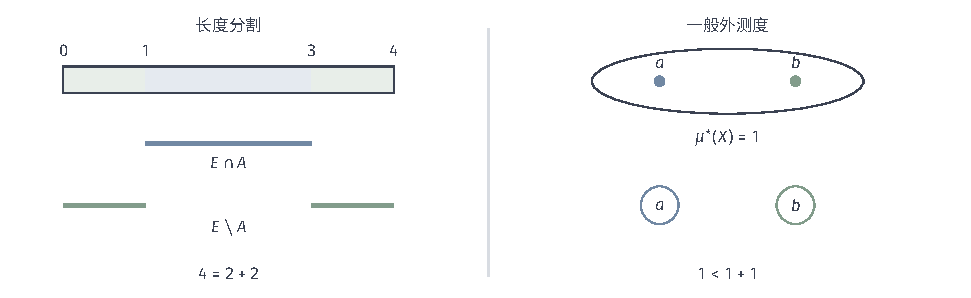
\includegraphics[width=169mm]{figures/01-mathematical-preliminaries-upper/01-mathematical-language-combinatorics-analysis-optimization/tikz/measure-exact-splitting/figure.pdf}
 \caption{精确分割与一般外测度的差别。左侧用$A=[1,3]$分割测试集$E=[0,4]$，落在$A$内的长度为$2$，外部两段总长度也为$2$，两者恢复原来的$4$；有限端点不改变长度。右侧使用正文两点空间的外测度，整体值为$1$，拆成两个单点后的值之和为$2$。右侧并非勒贝格不可测集的图像；左侧也只画了一个测试集，可测性定义要求对每个测试集都有精确等式。}
 \label{fig:measure-exact-splitting}
\end{figure*}

勒贝格外测度也存在不能保持精确分割的集合；这类不可测集的存在与构造可参考测度论教材\scite{math-hunter2011measure,math-folland1999real}，这里不展开。
下面直接以精确分割为条件选取可测集，并证明这类集合上的可加性。

\paragraph{可测集的定义}

我们希望$A$能够在不同范围的计算中反复参与分割，因此条件不能只针对某个预先选好的$E$。
下面要求等式对所有测试集成立，并把满足要求的$A$称为勒贝格可测集。
\begin{definition}[勒贝格可测集]
\label{def:analysis-lebesgue-measurable-set}
集合$A\subseteq\mathbb R$称为\term{勒贝格可测集}（Lebesgue measurable set），若对每个$E\subseteq\mathbb R$都有
\begin{equation}
 m^*(E)=m^*(E\cap A)+m^*(E\setminus A).
 \label{eq:comb-caratheodory-measurability}
\end{equation}
全体勒贝格可测集组成的集合族记为$\mathcal L(\mathbb R)$。
\end{definition}

这称为Carathéodory可测性条件。
由于其中一个不等式已经成立，验证可测性只需证明
$m^*(E)\geq m^*(E\cap A)+m^*(E\setminus A)$。
必须检验每个$E$，因为只令$E=A$会得到对任意集合都成立的恒等式，无法区分哪些分割与外测度相容。
“可测”并不表示此前无法给$A$求值；$m^*(A)$对任意$A$都已定义。新增要求是$A$与所有测试集的分割相容。

外测度为零的集合不需要逐个寻找特殊分割。下面先证明一个通用结论，以后处理零测余量和完备性时都可使用。
\begin{lemma}[零外测度集的子集可测]
\label{lem:analysis-zero-outer-measure-measurable}
若$N\subseteq\mathbb R$且$m^*(N)=0$，则每个$D\subseteq N$都勒贝格可测，并且$m^*(D)=0$。
\end{lemma}
\begin{proof}
单调性先给出$m^*(D)=0$。对任意测试集$E$，有
\[
 m^*(E\cap D)+m^*(E\setminus D)=0+m^*(E\setminus D)\leq m^*(E).
\]
结合外测度次可加性给出的反向不等式，得到可测性所需的精确分割等式。
\end{proof}
前面已证明$m^*(Q_0)=0$，所以此引理立即说明$Q_0$勒贝格可测。

后面把外测度限制到可测集上定义勒贝格测度时，$Q_0$的值仍为$0$。
取$E=[0,1]$还得到$m^*([0,1]\setminus Q_0)=1$：有理点与无理点都分布在每一小段中，却不因此占有相同的长度。
可测性由上述分割等式判断，而不是由集合看起来是否稠密、光滑或规则判断。

\subsubsection{可测集族}

前面的定义逐个检验一个集合能否精确切分任意测试集。接下来还要检验：这些可测集合经过取补、合并等运算后，是否仍然可测？

如果每次分块或合并都可能离开允许测量的范围，就无法反复使用这套测量方法。例如，每个单点$\{q_n\}$都Jordan可测，它们的可数并$Q_0$却不Jordan可测。
这说明允许每个部分参与测量，还不够保证合并后的对象也能参与测量。

勒贝格构造需要解决这个范围问题：先证明可测集族对所需运算封闭，再讨论合并后数值怎样相加。

\paragraph{取补与有限并}

取补对应保留分割的另一侧，有限并对应把有限块合为一块；先检查这两类操作，便能处理有限次分块计算。
下面始终以任意测试集$E$检验所得集合，沿用已经证明的次可加性作为其中一个方向。

空集满足$m^*(E)=0+m^*(E)$，所以可测。
把$A$换成$\mathbb R\setminus A$只交换式~\eqref{eq:comb-caratheodory-measurability}右边的两项，因此取补保持可测，特别地$\mathbb R$也可测。

若$A,B$可测，先用$A$分割$E$，再用$B$分割$E\setminus A$，得到
\[
 \begin{aligned}
 m^*(E)&=m^*(E\cap A)+m^*((E\setminus A)\cap B)\\
 &\quad +m^*(E\setminus(A\cup B))\\
 &\geq m^*(E\cap(A\cup B))+m^*(E\setminus(A\cup B)).
 \end{aligned}
\]
前两部分恰好组成$E\cap(A\cup B)$；次可加性使它们的外测度之和不小于这个并的外测度，得到所需反向不等式。
结合已有的次可加界，对每个$E$都有精确分割，所以$A\cup B$可测。
再由$A\cap B=(A^c\cup B^c)^c$和$A\setminus B=A\cap B^c$，得到有限交与差的可测性，这里的补集均相对于$\mathbb R$。
若$A,B$不交，以$A$分割$E\cap(A\cup B)$还给出
\[
 m^*(E\cap(A\cup B))=m^*(E\cap A)+m^*(E\cap B).
\]
反复应用可处理任意有限个不交可测集合。
这里同时得到了两件事：有限并仍在可测范围内；对不交的有限部分，切分前后的外测度精确相加。
后面处理可数并时，将先使用这两条有限结论，不预先假定无限情形已经成立。

\paragraph{可数并}

有限次合并已经不会离开可测范围，但一列集合的并未必能在有限步结束，仍需单独证明可数并的可测性。
证明的办法是先精确切出前$N$块，再让非负部分和随$N$增加，而不是直接调用尚未建立的测度可数可加性。
设$C_n$两两不交且可测，令$U_N=\bigcup_{n=1}^NC_n$、$U=\bigcup_{n=1}^{\infty}C_n$。
有限分割与外测度单调性给出，对每个$E$和每个$N$，
\[
 \begin{aligned}
 m^*(E)
 &=\sum_{n=1}^Nm^*(E\cap C_n)+m^*(E\setminus U_N)\\
 &\geq\sum_{n=1}^Nm^*(E\cap C_n)+m^*(E\setminus U).
 \end{aligned}
\]
因为$E\setminus U\subseteq E\setminus U_N$，上式对每个$N$都成立。
对非负部分和取上确界，便得到整列分割所需的下界；再用外测度的可数次可加性合并$E\cap C_n$，得到
\[
 m^*(E)\geq\sum_{n=1}^{\infty}m^*(E\cap C_n)+m^*(E\setminus U)
 \geq m^*(E\cap U)+m^*(E\setminus U).
\]
这就是$U$的可测性条件，故不交可测集的可数并可测。
若$A_n$不一定不交，令$C_1=A_1$、$C_n=A_n\setminus\bigcup_{j<n}A_j$。
每个$C_n$只用有限并与差集构成，所以已知可测；逐项去掉此前出现的部分，又使它们两两不交且并集不变。
对$C_n$应用刚才的结论，就证明了一般可数并仍可测。
至此，取补、有限并和可数并的运算都不会使我们离开$\mathcal L(\mathbb R)$。

\paragraph{$\sigma$代数}

刚才证明的封闭性质，正是后续反复分块和合并时需要的范围保证。
为了在其他对象集合上也使用同样的保证，下面把“包含全集、取补封闭、可数并封闭”统一定义为$\sigma$代数。
\begin{definition}[$\sigma$代数]
\label{def:analysis-sigma-algebra}
设$X$为集合。若子集族$\mathcal A\subseteq\mathcal P(X)$满足
\[
 \begin{gathered}
 X\in\mathcal A,\\
 A\in\mathcal A\Longrightarrow X\setminus A\in\mathcal A,\\
 A_1,A_2,\ldots\in\mathcal A
 \Longrightarrow\bigcup_{n=1}^{\infty}A_n\in\mathcal A,
 \end{gathered}
\]
则称$\mathcal A$为$X$上的\term{$\sigma$代数}（sigma-algebra）。
\end{definition}

由取补可得$\varnothing\in\mathcal A$；在有限集合族之后补空集，便得到有限并。
De Morgan公式又给出可数交：$\bigcap_nA_n=X\setminus\bigcup_n(X\setminus A_n)$。
可数交的封闭性也很实用：例如$\{a\}=\bigcap_{n\geq1}(a-1/n,a+1/n)$，一个点可以由一列邻域的交得到。
因此，只保证有限运算封闭还不能覆盖后面涉及无限过程的集合构造，$\sigma$代数将这些可数运算纳入同一个范围。

在当前的勒贝格构造中，$\mathcal L(\mathbb R)$先由精确分割条件选出，再由前面的推导证明它是$\sigma$代数；
没有先假定所有可测集合自动具有这些封闭性。
在抽象测量问题中，则可以先指定一个$\sigma$代数来规定允许测量的范围。
两种做法的起点不同，但得到的范围结构相同。

$\sigma$代数记录允许测量的子集，并保证这些子集经过所需的集合运算后仍在这一范围内；它没有给集合赋予大小，也没有单独保证任何数值的可加性。
所以接下来还要把已经构造的外测度放到这个可测范围上，证明它确实满足精确相加的规则。

\subsubsection{勒贝格测度}

\paragraph{限制外测度}

现在有了两个对象：$m^*$负责给集合赋值，$\mathcal L(\mathbb R)$负责保证取补和可数合并后仍在可测范围内。
我们保留$m^*$在可测集上的原值，把允许的输入从所有子集收缩为$\mathcal L(\mathbb R)$，并给这个限制后的赋值命名。
\begin{definition}[勒贝格测度]
\label{def:analysis-lebesgue-measure}
勒贝格外测度在$\mathcal L(\mathbb R)$上的限制
\[
 m:\mathcal L(\mathbb R)\to[0,\infty],\qquad m(A)=m^*(A),
\]
称为\term{勒贝格测度}（Lebesgue measure）。
\end{definition}

这一步没有重新计算任何可测集的大小：例如$m(Q_0)=m^*(Q_0)=0$，空集仍有$m(\varnothing)=0$。
改变的是赋值的定义域，而“它是测度”还需要下面的可数可加性证明。

\paragraph{不交可测并的可数可加性}

$\sigma$代数已经保证可数并是允许输入，因此等式左侧有定义；精确分割条件则使每个有限不交部分和都成为并集测量值的下界。
对这些下界取上确界，再结合外测度原有的次可加上界，就能把不等式收紧为等式。
\begin{theorem}[勒贝格测度的可数可加性]
\label{thm:analysis-lebesgue-countable-additivity}
若$A_n\in\mathcal L(\mathbb R)$两两不交，则
\[
 m\left(\bigcup_{n=1}^{\infty}A_n\right)=\sum_{n=1}^{\infty}m(A_n).
\]
\end{theorem}
\begin{proof}
记$A=\bigcup_n A_n$。前面已证明$A$可测；对每个$N$，由单调性与有限分割，
\[
 m(A)\geq m\left(\bigcup_{n=1}^NA_n\right)=\sum_{n=1}^Nm(A_n).
\]
对$N$取上确界，得到$m(A)\geq\sum_n m(A_n)$。
反向不等式正是外测度的可数次可加性，因为$m$与$m^*$在这些集合上相同。
\end{proof}

因此，可数并封闭与可数可加解决的是两个相接的问题：前者保证合并后的集合仍可测量，后者保证它的测量值等于不交部分之和。
从$m^*$到$m$也经过了两步：先由精确分割条件得到$\mathcal L(\mathbb R)$及其封闭性，再证明保留在这一范围上的数值具有可数可加性。
这两步共同使勒贝格测度能够用于反复的分块累计。
类似构造也适用于一般外测度；这里已经把一维长度所需的关键封闭性与可加性步骤给出，
更一般的表述可参考测度论教材\scite{math-hunter2011measure,math-folland1999real}。

\paragraph{区间与常见可测集}

可数可加性定理只适用于已经可测的集合，所以还要确认普通区间、开集等常用对象确实属于$\mathcal L(\mathbb R)$。
先从半直线开始：它只需在一个位置切分区间，容易将可测性条件还原为已知长度之和。

固定$t\in\mathbb R$，考虑半直线$H=(-\infty,t]$。
若$m^*(E)<\infty$，给定$\varepsilon>0$，选择总长度小于$m^*(E)+\varepsilon$的开区间覆盖$\{I_j\}$。
将每个$I_j$在$t$处切成两段；两段可能是开区间、半开区间或空集，
其外测度已知等于各自长度，而两段长度之和仍是$\ell(I_j)$。
分别覆盖$E\cap H$和$E\setminus H$，由外测度的次可加性得
\[
 \begin{aligned}
 &m^*(E\cap H)+m^*(E\setminus H)\\
 &\quad\leq\sum_j\bigl[m^*(I_j\cap H)+m^*(I_j\setminus H)\bigr]\\
 &\quad=\sum_j\ell(I_j)<m^*(E)+\varepsilon.
 \end{aligned}
\]
令$\varepsilon\downarrow0$就得到所需反向不等式。
若$m^*(E)=\infty$，次可加性已迫使分割后总和也为无穷，等式自动成立。
所以$H$可测。

半直线的差给出半开区间；可数并与交又给出其他端点型式的区间和单点。
任意开集是其中所有有理端点开区间的并：对每个点先取完全落在开集内的小区间，再利用有理数的稠密性缩小端点。
有理端点对可数，故这是一组可数并，所以开集、其补集及后续可数集合运算所得的集合都可测。
区间长度结论也随之保留为
\[
 m((a,b))=m([a,b])=m([a,b))=b-a,\qquad m(\{a\})=0.
\]

\paragraph{Borel集合}

区间与开集已经可测，但以后往往从它们出发反复取补、作可数并或可数交。
为了统一指明这些操作必然产生的集合，下面定义包含全部开区间的最小$\sigma$代数。

这样的最小范围确实存在：$\mathcal P(\mathbb R)$是一个包含所有开区间的$\sigma$代数，故候选不空。
把全部候选取交，所得集合族仍包含全集，并且取补、可数并后仍属于每个候选，所以交族本身也是$\sigma$代数。
它包含所有开区间，又包含于每个候选，因而正是所需的最小范围，称为由开区间生成的$\sigma$代数。
\begin{definition}[Borel $\sigma$代数]
\label{def:analysis-borel-sigma-algebra}
实轴上由所有开区间$(a,b)$（$a<b$）生成的最小$\sigma$代数记为$\mathcal B(\mathbb R)$，称为\term{Borel $\sigma$代数}（Borel sigma-algebra）。
对$X\subseteq\mathbb R$，令
\[
 \mathcal B(X)=\{X\cap B:B\in\mathcal B(\mathbb R)\},
\]
称为$X$上的Borel $\sigma$代数；其中的集合称为Borel集合。
\end{definition}

前面对开集的表示说明，这也等于所有开集生成的$\sigma$代数。
例如$\{a\}=\bigcap_{n\geq1}(a-1/n,a+1/n)$是Borel集合，可数点集因而也是Borel集合。
各范围之间有
\[
 \mathcal B(\mathbb R)\subseteq\mathcal L(\mathbb R)\subseteq\mathcal P(\mathbb R),
 \qquad m=m^*\big|_{\mathcal L(\mathbb R)}.
\]
第一个包含关系来自可测范围的封闭性：$\mathcal L(\mathbb R)$已经是包含所有开区间的$\sigma$代数，必包含最小的$\mathcal B(\mathbb R)$。
第二个包含关系只说明可测集也是实轴子集；它不表示全部子集都可测。
这里$\mathcal B(\mathbb R)$与$\mathcal L(\mathbb R)$都是集合族，规定允许的范围；$m$与$m^*$是给集合赋值的函数，职责不同。
勒贝格可测范围仍不是所有子集；不可测集的构造不在这里展开。

\paragraph{Jordan测量与勒贝格测度}

前面已经说明区间长度保持不变，现在进一步检验每个Jordan可测集是否都被新构造保留，且测量值相同。
证明中的零测余量由引理~\ref{lem:analysis-zero-outer-measure-measurable}处理：外测度为零的集合的任意子集都已可测，因此内部Borel部分之外的零测误差不会破坏可测性。

若$E$为Jordan可测集，对每个$n$取初等集$A_n\subseteq E\subseteq B_n$，
使$\ell(B_n)-\ell(A_n)<2^{-n}$。
令$A=\bigcup_nA_n$、$B=\bigcap_nB_n$，则$A,B$均为Borel集合，且$A\subseteq E\subseteq B$。
由于$B\setminus A\subseteq B_n\setminus A_n$，有
$m(B\setminus A)\leq\ell(B_n)-\ell(A_n)<2^{-n}$对所有$n$成立，故$m(B\setminus A)=0$。
该引理表明$E\setminus A$可测，于是$E=A\cup(E\setminus A)$也可测。
再由$j_*(E)\leq m(E)\leq j^*(E)$得到$m(E)=j(E)$。

因此Jordan可测集都勒贝格可测，数值保持一致；$Q_0$则说明逆向不成立。
它虽然在每个小区间中都稠密，却是可数Borel集合，勒贝格测度为零。
可测性的边界由分割性质规定，不由“看起来复杂”来判定。

\subsection{测度空间与测度的性质}
\label{sec:comb-measurable-sets-and-weights}

勒贝格长度已经形成一套完整的测量设定：实轴$\mathbb R$给出对象范围，$\mathcal L(\mathbb R)$给出允许测量的子集族，$m$给这些子集赋值。
有限加权计数也具有相同的三层结构，只是对象范围和具体赋值不同。

为了把后面的推导同时用于长度、计数与其他权重，现在把三层结构分别抽象出来。
先记录对象范围和可测集合族，得到可测空间；再要求赋值满足空集为零与可数可加性，得到测度；
将三项放在一起才得到测度空间。之后有关集合列与零测例外的结论，就可以从共同条件推出，不必对每一种测量重新证明。

这里改变的是讨论范围：此前通过区间覆盖构造了一个特定的函数$m$，现在将它已满足的性质提炼为一般赋值的共同要求。
勒贝格测度本身的定义和值都不改变；它成为一般测度的一个实例，计数和其他权重也能纳入同一套结论。
一般测度不必从实轴区间覆盖出发构造，也不必把区间赋值为长度。
图~\ref{fig:measure-abstraction}将这条具体构造与抽象过程分开，并对照三项结构。

\begin{figure*}[htbp]
 \centering
 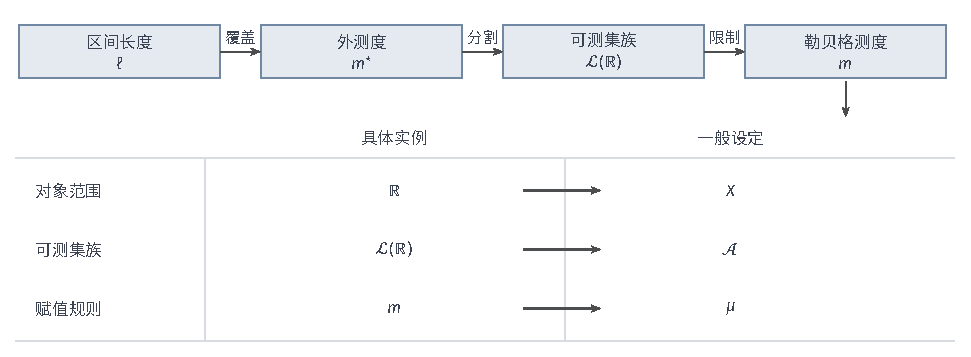
\includegraphics[width=169mm]{figures/01-mathematical-preliminaries-upper/01-mathematical-language-combinatorics-analysis-optimization/tikz/measure-abstraction/figure.pdf}
 \caption{从勒贝格测度到一般测度。上部是前文在实轴上完成的具体构造：区间长度经可数覆盖得到外测度，再用精确分割选出可测集，将外测度限制到这一集合族上得到$m$。中部将对象范围、允许集合族与赋值规则对应为$X$、$\mathcal A$、$\mu$，其中$\mathcal A$为$X$上的$\sigma$代数，$\mu:\mathcal A\to[0,\infty]$。测度$\mu$须满足空集为零和两两不交可测集合的可数可加性。前两项组成可测空间$(X,\mathcal A)$，三项共同组成测度空间$(X,\mathcal A,\mu)$。在同一$(\mathbb R,\mathcal L(\mathbb R))$上，勒贝格测度$m$给单点赋值$0$，计数测度$\nu$则赋值$1$，说明允许测量的集合相同，赋值仍可不同。因此勒贝格测度是一种具体测度，一般测度的定义不限定为长度，也不要求都按上部的区间覆盖步骤构造。}
 \label{fig:measure-abstraction}
\end{figure*}


\subsubsection{测度空间}

\paragraph{可测空间}

只给出集合$X$，还没有指定哪些子集可以参与测量；允许范围需要单独记录，并应对取补和可数并封闭。
因此，下面把$X$与它上面选定的$\sigma$代数组合起来，暂不指定任何测量值。

\begin{definition}[可测空间]
设$\mathcal A$为$X$上的$\sigma$代数，二元组$(X,\mathcal A)$称为\term{可测空间}（measurable space）。
$\mathcal A$中的集合称为相对于$\mathcal A$的\term{可测集合}（measurable set）。
\end{definition}
例如$X=\{a,b,c\}$上的
$\mathcal A=\{\varnothing,\{a,b\},\{c\},X\}$是一个$\sigma$代数。
这个例子把$a,b$作为不能单独分开的同一块，而$c$单独成块；列出的集合就是这些块的各种并。
取补会选出剩余块，可数并也仍是这些块的并，所以$\mathcal A$确实是$\sigma$代数。
在这个可测空间中，$\{a,b\}$属于允许范围，$\{a\}$却不属于它。
这只表示当前没有把$\{a\}$列为可测对象，并不表示它在任何测量设定下都不能测量；改选$\mathcal P(X)$就会允许全部子集。

所以，抽象可测空间中的“可测”是相对于指定的$\mathcal A$而言的。
前面的“勒贝格可测”则指通过$m^*$的精确分割条件得到的特定范围$\mathcal L(\mathbb R)$；它为一般定义提供了一个已经证明满足要求的实例。

\paragraph{测度}

可测空间保证集合运算后的对象仍在允许范围内，却还没有给任何集合规定数值。
下面借鉴已经证明的勒贝格可数可加性，对一般赋值提出同样要求；右侧仍用非负级数求和，允许值为$+\infty$。
\begin{definition}[测度]
设$(X,\mathcal A)$为可测空间。映射$\mu:\mathcal A\to[0,\infty]$若满足$\mu(\varnothing)=0$，并且对任意两两不交的$A_1,A_2,\ldots\in\mathcal A$有
\begin{equation}
 \mu\left(\bigcup_{n=1}^{\infty}A_n\right)
   =\sum_{n=1}^{\infty}\mu(A_n),
 \label{eq:comb-countable-additivity}
\end{equation}
则称$\mu$为\term{测度}（measure），这个等式称为可数可加性。
\end{definition}

\paragraph{测度空间}

确定$X$和$\mathcal A$以后，具体的赋值规则仍未唯一确定，例如同一有限集合可以采用每点计一，也可以采用不同点权重。
为了完整指明一次测量使用的对象、允许范围和赋值，下面把测度也加入记录。

\begin{definition}[测度空间]
\label{def:analysis-measure-space}
设$\mu$为可测空间$(X,\mathcal A)$上的测度，三元组$(X,\mathcal A,\mu)$称为\term{测度空间}（measure space）。
\end{definition}
同一可测空间可以有不同的测度。例如在$X=\{a,b\}$的全部子集上，
权重$(1,1)$给出$\mu(X)=2$，权重$(1,2)$给出$\mu(X)=3$；两种都满足可数可加性。
不交分割只把原来的非负项重新分组，不会改变它们的总量。
因此，$\sigma$代数与测度不能互相代替：前者决定哪些集合可以测量，后者决定这些集合有多大。
勒贝格测度空间写成$(\mathbb R,\mathcal L(\mathbb R),m)$；下面的计数、点质量与可数加权计数则给出其他完整例子。

\paragraph{计数测度}

一般测度不必表示长度；若只关心集合中有多少个元素，可以保留有限计数，并将无限集合统一记为总量无穷。
在任意集合$X$的幂集上，定义
\[
 \mu(A)=\begin{cases}|A|,&A\text{有限},\\+\infty,&A\text{无限},\end{cases}
\]
称为\term{计数测度}（counting measure）。对两两不交的集合，有限时各元素恰计一次；
并集无限时，若某部分无限，右侧已有一项为无穷；
若各部分有限，就必须有无限多个非空部分，右侧至少包含无限多个$1$，仍为无穷。因而满足可数可加性。
例如自然数上的计数测度给单点赋值$1$，给整个自然数集赋值$+\infty$。

\paragraph{点质量}

计数对每个点赋予相同权重；若只想记录一个指定点是否落在集合中，可以把全部权重集中到这个点。
固定$a\in X$，在$\mathcal P(X)$上定义包含$a$的集合测度为$1$，不包含$a$的集合测度为$0$，
得到集中在$a$的\term{点质量}（point mass）测度，记为$\delta_a$。
例如对$b\neq a$，有$\delta_a(\{a,b\})=1$、$\delta_a(\{b\})=0$。
一族不交集合中至多一个包含$a$，所以这也是测度。

\paragraph{可数加权计数}

有限集合上的加权计数也可以沿用级数规则扩展。
对互异的可数个点$x_n$赋权$w_n\geq0$，在$X=\{x_n:n\geq1\}$的全部子集上定义
\[
 \mu(A)=\sum_{n:x_n\in A}w_n.
\]
不交集合把非负项分成不重复的索引组；由有限子集和的上确界表示，分组求和与直接累计相同，所以满足可数可加性。
例如$X=\mathbb N_+$、$w_n=2^{-n}$时，$\mu(X)=1$；改为$w_n=1$则得到计数测度。
这仍是逐点赋权；勒贝格长度则处理不能逐点列举的区间，二者共享测度公理，但构造方式不同。
现在已经可以将它们放在同一框架内：每个例子都指定对象集合、一个$\sigma$代数及其上的测度，
接下来只用这些共同条件推导基本性质，不再依赖它们各自怎样构造。

\subsubsection{基本性质与集合列}
\label{sec:comb-set-approximation}
\label{sec:analysis-set-measure-continuity}

测度的定义只直接规定了不交可数并的数值。实际计算还会遇到包含、重叠以及逐步扩大或缩小的集合，需要把这些关系转成已经能够处理的不交分割。
下面先由分割得到大小比较和重叠集合的上界，再研究一列集合的并、交与测量值极限的关系。
这些结论对任意测度空间$(X,\mathcal A,\mu)$都成立，不依赖实轴的区间结构。

\paragraph{单调性}

如果$A\subseteq B$，较大的集合只比$A$多出$B\setminus A$这一部分。对可测的$A,B$，差集也可测，且两部分不交，因此
\[
 \mu(B)=\mu(A)+\mu(B\setminus A)\geq\mu(A).
\]
这称为测度的单调性，说明包含关系能给出测量值的上下界。
若$\mu(B)<\infty$，还可以写成$\mu(B\setminus A)=\mu(B)-\mu(A)$，用总量减去已知部分计算余量。
这里的有限性不能省略：可加等式允许无穷值，相减却不能出现$\infty-\infty$。

\paragraph{次可加性}

集合有重叠时，直接相加会重复计算。对可测集合列$A_n$，把每一步已经出现的部分去掉，令
\[
 B_1=A_1,\qquad B_n=A_n\setminus\bigcup_{j<n}A_j\quad(n\geq2).
\]
$B_n$仍可测、两两不交，且与原集合列有相同的并；又有$B_n\subseteq A_n$，故
\[
 \mu\left(\bigcup_nA_n\right)=\sum_n\mu(B_n)\leq\sum_n\mu(A_n).
\]
这就是可数次可加性：即使无法消除所有重叠，也能用各部分测度之和控制并集的测度。
它还说明可数个可测零测集的并仍是零测集，因为右侧此时为$0$；后面合并例外范围时会用到这一点。

若$A,B$的测度有限，把两者分成$A\setminus B$、$A\cap B$与$B\setminus A$，还可精确校正重复部分，得到
\[
 \mu(A\cup B)=\mu(A)+\mu(B)-\mu(A\cap B).
\]
这是测度形式的容斥公式。有限性保证其中的相减有意义。

\paragraph{递增集合列}

有时一个范围是逐步加入新部分形成的，例如用越来越多的区间逼近一个开集。此时要知道，每一步的测量值能否确定最终并集的测量值。
若$A_1\subseteq A_2\subseteq\cdots$且$A=\bigcup_nA_n$，记为$A_n\uparrow A$。
可测范围对可数并封闭，所以$A$可测；下面说明数值也能取极限。

增量$B_1=A_1$、$B_n=A_n\setminus A_{n-1}$两两不交，且
$A_n=\bigcup_{j=1}^nB_j$、$A=\bigcup_{j=1}^{\infty}B_j$。
于是可数可加性把集合逐步增加转成非负部分和逐步增加，得到
\begin{equation}
 \mu(A)=\sup_{n\geq1}\mu(A_n)=\lim_{n\to\infty}\mu(A_n).
 \label{eq:comb-measure-continuity-below}
\end{equation}
这个结论称为测度的下连续性，不要求$\mu(A)$有限；非负部分和的极限也可以是$+\infty$。
例如在勒贝格测度下，$A_n=(0,1-1/n)$递增，并集为$(0,1)$，各步长度趋于$1$，正好等于并集长度。

\paragraph{递减集合列}

逐步去掉部分时，最终留下的是交集。若$A_1\supseteq A_2\supseteq\cdots$且$A=\bigcap_nA_n$，记为$A_n\downarrow A$。
交集可测，但要由各步测度恢复交集测度，还需要一个有限总量作为相减的起点。

设$\mu(A_1)<\infty$。把留下的范围改为已经去掉的范围，$A_1\setminus A_n$便递增到$A_1\setminus A$。
应用下连续性，再利用所有集合都包含在有限测度的$A_1$中，得到
\[
 \mu(A_1)-\mu(A)=\lim_{n\to\infty}\bigl[\mu(A_1)-\mu(A_n)\bigr].
\]
所有减法都在有限数值间进行，整理后有
\begin{equation}
 \mu(A)=\inf_{n\geq1}\mu(A_n)=\lim_{n\to\infty}\mu(A_n).
 \label{eq:comb-measure-continuity-above}
\end{equation}
这称为测度的上连续性。若只有某个$A_{n_0}$的测度有限，舍去它之前的有限项，也能应用同一结论。

例如$[0,1/n]\downarrow\{0\}$，长度递减趋于$0$。
有限性条件确有作用：$(n,\infty)\downarrow\varnothing$，但每项长度均为无穷，测量值没有记录这些范围正在向远处移走，因而不能由下确界得到空集长度。
图~\ref{fig:vol1-add-nested-set-limits}对照递增、有限测度下递减及缺少有限性时失败的三种情形。
\begin{figure}[!htb]
  \centering
  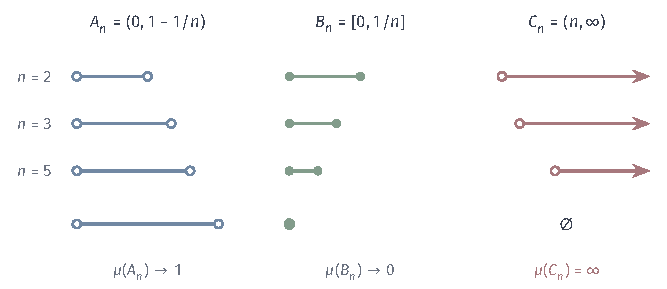
\includegraphics[width=112mm]{figures/01-mathematical-preliminaries-upper/01-mathematical-language-combinatorics-analysis-optimization/tikz/comprehension-additions/nested-set-limits.pdf}
  \caption{实轴上的三列嵌套集合，依次画$n=2,3,5$及最终的并集或交集，均使用勒贝格测度。左列$A_n$递增，并集为$(0,1)$；中列$B_n$递减，交集为$\{0\}$；右列$C_n=(n,\infty)$递减，交集为空，而每一项的测度仍为无穷。空心、实心端点分别表示不包含、包含；各列仅在本列内共用坐标尺度。}
  \label{fig:vol1-add-nested-set-limits}
\end{figure}
\FloatBarrier

\subsubsection{零测集与完备性}
\label{sec:comb-null-sets-and-completion}

集合差的测度可以描述遗漏或多出的总量。当这份总量恰为零时，函数仍可能在其中某些点取不同值，某个性质也可能在那里失效。
我们需要分别说明什么是零测范围、怎样表达范围内允许有例外，以及这些例外的任意子集是否都在可测范围内。
前两个问题引出零测集和几乎处处，最后一个问题引出完备性与完备化。

\paragraph{零测集}

测度为零不等于没有元素：勒贝格长度给单点赋值$0$，点本身却仍然存在。
为了用测量值而非点数描述这种范围，先给它一个名称。
\begin{definition}[零测集]
\label{def:analysis-null-set-almost-everywhere}
在测度空间$(X,\mathcal A,\mu)$中，若$N\in\mathcal A$且$\mu(N)=0$，称$N$为\term{零测集}（null set）。
\end{definition}
单点与所有可数点集在勒贝格测度下都是零测集，因为可数次可加性或次可加性使这些单点的总量仍为零。
在计数测度下，单点的测度却是$1$，唯一的零测集是空集。
因此说一个集合“零测”时，必须同时明确采用什么测度。

\paragraph{几乎处处}

比较两个函数时，除了判断它们是否逐点相等，还可以考察它们不同的位置是否都落在一个零测集中。
下面用同样的方式描述一般性质的例外范围，同时保留所用测度的信息。
\begin{definition}[几乎处处]
若存在可测零测集$N$，使某性质对每个$x\in X\setminus N$成立，称该性质$\mu$-\term{几乎处处}（almost everywhere，简写为a.e.）成立。
\end{definition}
例如$f(0)=1$、$f(x)=0$（$x\neq0$）与恒零函数在勒贝格测度下几乎处处相等，尽管它们在$0$处并不相等。
更进一步，$f=\mathbb I_{Q_0}$在$[0,1]$上也几乎处处等于零，因为例外都在有理点集$Q_0$内。
例外可以在每一小段中出现，所以“几乎处处”不表示只遗漏有限个点，也不表示每个位置附近都没有例外。
按前面有理与无理点的分布，这个指示函数处处不连续，而恒零函数处处连续；几乎处处相等也不会自动保留连续性或某个指定点的取值。
后面讨论积分和函数空间时，会明确哪些结论只依赖零测范围之外的取值。

若一列性质分别在零测集$N_1,N_2,\ldots$之外成立，那么它们在$\bigcup_nN_n$之外同时成立；这个并仍零测。
这使可数多项几乎处处结论能够使用共同的例外范围，但不能直接推广到不可数多项结论。
例如在$[0,1]$上，对每个$t\in[0,1]$，性质$x\neq t$都在勒贝格测度下几乎处处成立；若要求它对所有$t$同时成立，却没有任何$x\in[0,1]$满足。

定义只要求实际例外集包含在某个可测零测集$N$中，没有预先要求例外集自身可测。
这样写是因为一般测度空间可能尚未纳入$N$的全部子集；下面的完备性正要处理这个问题。
计数测度下则没有非空零测例外，几乎处处成立就是处处成立。

\paragraph{Cantor集}
\label{sec:analysis-cantor-set}

可数集是熟悉的勒贝格零测集，但零测是否意味着最多只有可数多个点，还需另行检验。
下面的Cantor集说明，点的数量和长度为零是两种不同的信息。

由$[0,1]$反复删去每段的中间三分之一，得到的\term{Cantor集}（Cantor set）$C$是各层保留集合的交。
第$n$层由$2^n$个长$3^{-n}$的闭区间组成，因此$C$是Borel集合，并满足$m(C)\leq(2/3)^n$对所有$n$成立，故$m(C)=0$。

每条零一序列都可以改写为只用数字$0,2$的三进制数，所得点在$C$中。
两个序列首个不同位的差为$2\cdot3^{-k}$，其后位数的总差至多$3^{-k}$，因此给出不同点。
零一序列不可数：假定列出全部序列，把第$n$条序列的第$n$位取反就得到遗漏的一条。
所以$C$是不可数零测集。零测例外能够包含不可数多个点，几乎处处的表述因此不能用“除去可数多个点”替代。


图~\ref{fig:analysis-process-cantor-deletion}画出上述删除过程：每一步仍有正长度，但这些长度可共同压到任意小，交集却仍保留点。
\begin{figure}[!htbp]
 \centering
 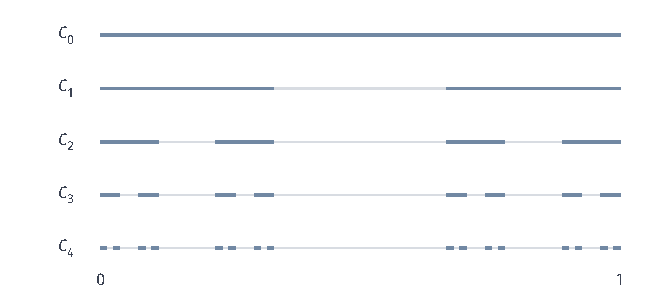
\includegraphics[width=112mm]{figures/01-mathematical-preliminaries-upper/01-mathematical-language-combinatorics-analysis-optimization/tikz/chapter3-concept-processes/cantor-deletion.pdf}
 \caption{蓝线表示$C_0,\ldots,C_4$，每一步从上一行各闭区间中删去中间开三分之一。$C_n$由$2^n$个长度$3^{-n}$的闭区间组成，总长度为$(2/3)^n$；交集$C$的测度因此为零，但始终包含$0,1$。任何有限一行仍有正测度，不能把有限阶段当成最终零测集。}
 \label{fig:analysis-process-cantor-deletion}
\end{figure}

\paragraph{完备性}

设$N$可测且$\mu(N)=0$。若其子集$D\subseteq N$也可测，单调性立即给出$\mu(D)=0$；问题在于$D$未必属于原来的$\mathcal A$。
下面把“所有这种子集都已纳入允许范围”作为一个单独要求。
\begin{definition}[完备测度空间]
\label{def:analysis-complete-measure-space}
若测度空间$(X,\mathcal A,\mu)$中每个零测集$N$的任意子集$D\subseteq N$都属于$\mathcal A$，称该测度空间完备。此时单调性给出$\mu(D)=0$。
\end{definition}
这里的完备性解决零测子集的可测资格，与度量空间中“柯西列是否有域内极限”的完备性是两种不同要求。

例如$X=\{a,b,c\}$、$\mathcal A=\{\varnothing,\{a,b\},\{c\},X\}$，给$\{a,b\}$测度$0$、$\{c\}$测度$1$。
按两块的不交加法确定其他值，就得到一个测度；但$\{a\}\subseteq\{a,b\}$且$\{a\}\notin\mathcal A$，所以它不完备。
在这个空间中，“$x\neq a$”仍几乎处处成立，因为例外被可测零测集$\{a,b\}$包住；此时却不能写$\mu(\{a\})=0$，因为$\mu$尚未在$\{a\}$上定义。
完备空间会消除这种资格上的缺口：被可测零测集包住的例外集自身也可测且为零测。

\paragraph{完备化}

若测度空间不完备，我们希望加入缺少的零测子集，同时保留原来各集合的测量值。
只把零测子集逐个加入还不够，新的允许范围还必须是$\sigma$代数，所以也要允许它们与原可测集组合。

具体把新集合写成“原可测部分$A$加上零测范围内的一部分$D$”，并让$D$不增加总量。
由此定义下面的扩展，随后检查赋值、封闭性和可加性确实成立。
\begin{definition}[测度空间的完备化]
在测度空间$(X,\mathcal A,\mu)$上，令
\[
 \begin{aligned}
 \overline{\mathcal A}&=\left\{A\cup D:
 \begin{array}{l}A,N\in\mathcal A,\quad\mu(N)=0,\\D\subseteq N\end{array}\right\},\\
 \bar\mu(A\cup D)&=\mu(A).
 \end{aligned}
\]
所得$(X,\overline{\mathcal A},\bar\mu)$称为原测度空间的\term{完备化}（completion）。
\end{definition}
取$D=\varnothing$便保留所有原可测集及其测度，取$A=\varnothing$便纳入所有原零测集的子集。
在三点例子中，这会加入$\{a\},\{b\}$及它们与$\{c\}$的并，得到全部子集；原来两块的测度仍为$0$与$1$。

首先要检查同一新集合的不同表示不会给出不同数值。
若$A\cup D=A'\cup D'$，其中$D\subseteq N$、$D'\subseteq N'$，则可测差集$A\setminus A'\subseteq N'$、$A'\setminus A\subseteq N$都为零测。
把$A,A'$各拆成公共部分与差集，有限可加性给出$\mu(A)=\mu(A\cap A')=\mu(A')$，即赋值与表示无关；这里没有使用可能无意义的无穷值相减。

其次检查新的范围对所需运算封闭。全集已在原范围内；取补时，
\[
 X\setminus(A\cup D)=[X\setminus(A\cup N)]\cup[N\setminus(A\cup D)],
\]
第一项原本可测，第二项是原可测零测集$N$的子集，仍是允许的新表示。
可数并也保持这种形式：$\bigcup_j(A_j\cup D_j)=(\bigcup_jA_j)\cup(\bigcup_jD_j)$，
而$\bigcup_jD_j\subseteq\bigcup_jN_j$，右侧是原可测零测集。
所以$\overline{\mathcal A}$确实是$\sigma$代数。

再检查测量规则。若$A_j\cup D_j$两两不交，它们的可测部分$A_j$也两两不交，故
\[
 \bar\mu\left(\bigcup_j(A_j\cup D_j)\right)
 =\mu\left(\bigcup_jA_j\right)
 =\sum_j\mu(A_j)=\sum_j\bar\mu(A_j\cup D_j).
\]
空集的值也仍为零，因此$\bar\mu$是测度。
若新可测集$A\cup D$的测度为零，则$\mu(A)=0$，整个集合包含在原可测零测集$A\cup N$中。
它的任意子集都已按新规则纳入，故扩展后的空间完备。

这些加入也是必要的：任何保留原测度的完备扩展，都必须包含原零测集的所有子集及它们与原可测集的并。
所以完备化给出的正是满足这一要求所需的最小可测范围，并未任意改变已有测量规则。
引理~\ref{lem:analysis-zero-outer-measure-measurable}已经保证勒贝格零测集的全部子集可测且仍零测，所以勒贝格测度本身已经完备。
接下来将用集合逼近说明：从Borel长度出发进行完备化，恰好得到完整的勒贝格可测范围。

\subsubsection{集合的逼近}

集合列的连续性回答了“给定一列嵌套集合，最终并或交有多大”；现在要反过来问：给定一个可测集，能否为它找到容易描述的近似集合？
开集、闭集和有限区间并可以用区间或有限组合描述，若能控制它们与原集合之间多出、漏掉部分的测度，就能把一般集合的问题转为简单集合的计算。

下面回到实轴上的勒贝格测度，使用它的开区间覆盖构造与实轴拓扑。
这些内外逼近不是任意测度空间自动具有的性质；一般的$(X,\mathcal A,\mu)$甚至还没有指定开集、闭集的含义。

\paragraph{内外正则性}

从外面逼近要求开集$O$包含全部$E$，只允许多出少量测度；从里面逼近要求有界闭集$K$完全落在$E$内，只允许漏掉少量测度。
下面把“少量”写成任意正误差，并保留控制余量所需的有限测度条件。
\begin{theorem}[有限测度集合的内外逼近]
设$E\in\mathcal L(\mathbb R)$且$m(E)<\infty$。对任意$\varepsilon>0$，存在开集$O$和有界闭集$K$满足
\begin{equation}
 K\subseteq E\subseteq O,\qquad
 m(O\setminus E)<\varepsilon,\qquad m(E\setminus K)<\varepsilon.
 \label{eq:comb-lebesgue-set-approximation}
\end{equation}
\end{theorem}
这就是本处使用的勒贝格测度正则性。这里控制的是多出、漏掉的测度，不要求集合边界在距离意义下彼此接近。
例如$E=[0,1]$可取$K=[0,1]$、$O=(-\varepsilon/3,1+\varepsilon/3)$，外面多出的长度为$2\varepsilon/3$，里面没有遗漏。

\begin{proof}
先作外逼近。由$m(E)=m^*(E)$的覆盖定义，选择总长度小于$m(E)+\varepsilon$的开区间覆盖，令$O$为这些区间的并。
它是可测开集，且$E\subseteq O$、$m(O)\leq\sum_j\ell(I_j)<m(E)+\varepsilon<\infty$。
把$O$分成不交的$E$与$O\setminus E$，可得$m(O\setminus E)=m(O)-m(E)<\varepsilon$。

内逼近分两步处理：先控制远处尾部，再在有限区间内对补集作外逼近。
因为$E\cap[-M,M]\uparrow E$，下连续性及$m(E)<\infty$保证可以取正整数$M$使
$m(E\setminus[-M,M])<\varepsilon/2$。
令$F=[-M,M]\setminus E$，它可测且测度有限。
应用刚才的外逼近，选开集$U\supseteq F$使$m(U\setminus F)<\varepsilon/2$，并令
\[
 K=[-M,M]\setminus U.
\]
$K$是有界闭集；由于已经去掉整个$F$，它包含于$E$。
遗漏部分分为区间外的尾部与区间内落入$U$的部分，因而
\[
 \begin{aligned}
 m(E\setminus K)
 &\leq m(E\setminus[-M,M])+m(U\setminus F)\\
 &<\varepsilon/2+\varepsilon/2=\varepsilon.
 \end{aligned}
\]
这就同时给出内外两种估计。
\end{proof}
有限性在证明中用于控制远处尾部并允许相减。若$E=\mathbb R$，任取有界闭集$K$，都有$m(E\setminus K)=\infty$，不可能达到上述任意小遗漏要求。
所以不能将本定理中“有界闭集的内逼近”直接照搬到无限测度集合；处理一般集合时，可以先限制在$[-M,M]$中作局部逼近。

图~\ref{fig:measure-inner-outer}将多出与漏掉的范围放在同一坐标尺度下。孤立点虽须包含于外覆盖，却可能在内逼近中被遗漏而不增加测度误差。

\begin{figure*}[htbp]
 \centering
 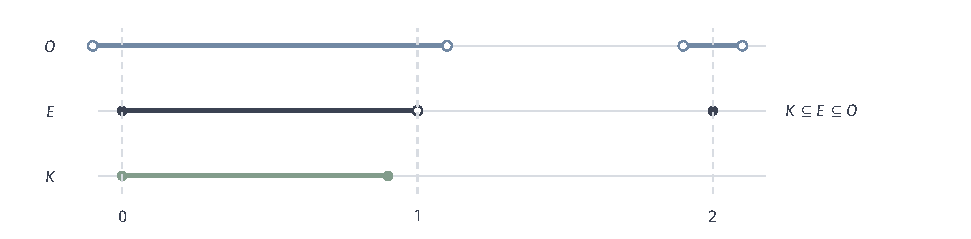
\includegraphics[width=169mm]{figures/01-mathematical-preliminaries-upper/01-mathematical-language-combinatorics-analysis-optimization/tikz/measure-inner-outer/figure.pdf}
 \caption{内外逼近控制的是集合差的测度。取$E=[0,1)\cup\{2\}$、有界闭集$K=[0,0.9]$及开集$O=(-0.1,1.1)\cup(1.9,2.1)$，有$K\subseteq E\subseteq O$。外面多出的长度$m(O\setminus E)=0.4$，里面遗漏的长度$m(E\setminus K)=0.1$；遗漏孤立点$2$不增加长度。空心端点不包含，实心端点包含。该图给出一次具体逼近，任意小误差由正文定理保证。}
 \label{fig:measure-inner-outer}
\end{figure*}


\paragraph{有限区间并}

开集和有界闭集仍可能包含无限结构。为了得到真正有限的计算对象，还希望用有限个区间的并逼近$E$。
这里改为同时控制多出和漏掉的总量，不要求这个有限区间并一定包含$E$或包含于$E$。

若$E=\varnothing$，直接取空集作为有限区间并即可。以下设$E$非空且可测、$m(E)<\infty$，给定$\varepsilon>0$，先取开集$O\supseteq E$使$m(O\setminus E)<\varepsilon/2$。
此时$m(O)<\infty$。把$O$写成其中有理端点开区间的可数并，令$O_N$为前$N$个区间之并，则$O_N\uparrow O$。
由下连续性，$m(O_N)\to m(O)$；总量有限，便有$m(O\setminus O_N)\to0$。
可选$N$使$m(O\setminus O_N)<\varepsilon/2$。
若所用区间只有有限个，可以重复已有区间补成一列。

记所得有限区间并为$B=O_N$。两方向的误差分别满足
$E\setminus B\subseteq O\setminus O_N$、$B\setminus E\subseteq O\setminus E$。
将它们合在一起，定义对称差$E\triangle B=(E\setminus B)\cup(B\setminus E)$，便有
\[
 m(E\triangle B)=m(E\setminus B)+m(B\setminus E)<\varepsilon.
\]
这称为在测度意义下逼近：误差是两集合不同之处的测度，而不是点的位置误差。
它与Jordan内外夹逼的要求不同。例如$E=Q_0$时，取$B=\varnothing$就有$m(E\triangle B)=0$，尽管两个集合并不相等。
这不构成Jordan外部逼近，因为空集并没有覆盖$Q_0$；所以这里的有限区间并逼近不与前面Jordan外容量为$1$的结论矛盾。
集合的这种逼近也不自动保证任意函数的积分误差很小，后面还需要对函数另加控制条件。

\paragraph{Borel范围的完备化}

完备化规定怎样加入零测子集，内外逼近则能说明一般勒贝格可测集与Borel集合究竟差在哪里。
下面证明每个勒贝格可测集都能写成Borel集合加上Borel零测集的一部分，因此Borel长度的完备化正好得到勒贝格范围。

先设$m(E)<\infty$。对每个$n$选有界闭集$K_n\subseteq E$使$m(E\setminus K_n)<2^{-n}$，令
\[
 F=\bigcup_{n=1}^{\infty}K_n.
\]
$F$是Borel集合且$F\subseteq E$。由于$E\setminus F\subseteq E\setminus K_n$对每个$n$成立，
$m(E\setminus F)\leq2^{-n}$对所有$n$成立，所以$m(E\setminus F)=0$。
这已给出一个内部Borel部分，但完备化的定义还要求把余量放入原范围中的零测集，因此需进一步找一个Borel零测集来包住它。

记$D=E\setminus F$。由外逼近，对每个$n$取开集$O_n\supseteq D$使$m(O_n)<2^{-n}$。
令$N=\bigcap_nO_n$，则$N$是Borel集合、$D\subseteq N$，且$m(N)\leq m(O_n)<2^{-n}$对所有$n$成立，故$m(N)=0$。
于是$E=F\cup D$，其中$F$为Borel集合，$D$包含于Borel零测集$N$，正是完备化允许加入的形式。

若$m(E)$无限，先对每个$E_k=E\cap[-k,k]$作上述构造，写成$E_k=F_k\cup D_k$、$D_k\subseteq N_k$。
取$F=\bigcup_kF_k$、$D=\bigcup_kD_k$、$N=\bigcup_kN_k$，便有$E=F\cup D$、$D\subseteq N$，
其中$F,N$均为Borel集合，$N$由可数次可加性仍为零测。
因此每个勒贝格可测集都进入Borel长度测度的完备化。

反过来，Borel集合已经勒贝格可测，Borel零测集的任意子集又因勒贝格完备性而可测，
所以完备化加入的集合不会超出勒贝格范围。
两个方向合起来证明，实轴上的勒贝格测度空间就是Borel长度测度空间的完备化，已有Borel集合上的长度保持不变。

到此，可数可加性使集合列的测度可以取极限，零测集给出几乎处处的例外语言，完备化补齐这类例外的子集，
内外逼近则把一般可测集联系到开闭集和有限区间并，并解释了Borel范围与勒贝格范围的关系。
下一节建立积分时，将使用这些可测范围、测量值以及控制误差的工具来累计函数取值。

\FloatBarrier

\section{一元函数的可测性和积分}
\label{sec:analysis-measurability-integration}
\label{sec:analysis-integration-average}
\label{sec:analysis-classical-integration}

上一节已经回答怎样测量集合的大小，现在进一步问：函数在不同位置取不同值时，怎样结合这些值与所在范围的大小，得到一个累计量？
例如，密度恒为$c$的一段区间长为$\ell$，总质量就是$c\ell$；密度随位置变化时，需要把这种计算推广到一般函数。
本节的自变量始终是一维实变量，有限区间先取$a<b$。

先沿输入区间分段取样，建立黎曼积分，检验分割越来越细时取样结果能否稳定。
狄利克雷函数将说明，有些函数的非零取值虽然只落在零测集上，每个短区间的取样却仍可能给出完全不同的累计。
为处理这种情形，我们利用第~\ref{sec:comb-set-measurement}节的可测集合与测度，改按函数取值划分输入，
先定义哪些函数能够这样分层，再以简单函数的有限累计构造勒贝格积分。

这条路线中的条件各有作用：可测集合提供允许测量的范围，测度给这些范围赋值，可测函数保证取值分层落在该范围内，
可积条件再保证总累计有限。它们不能互相替代。
在两种积分的定义和关系明确后，我们再研究累计函数与求导的联系、有限运算、函数列与函数项级数的极限交换以及反常积分；每一步都说明所用的是哪种积分及相应条件。

\subsection{黎曼定积分}
\label{sec:analysis-integral-definitions}
\label{sec:analysis-riemann-integral}

先保留区间长度作为权重，研究把输入切成小段后能否得到与取样无关的总量。这里使用有限区间分割，尚不需要一般可测集合的积分。


\subsubsection{积分的定义}

从常数密度乘长度的计算出发，先构造有限近似，再用所有足够细的近似是否稳定来定义积分。误差控制必须同时覆盖分割与取样两种选择。


\paragraph{区间分割}
要累计$f$在$[a,b]$上的取值，先把区间分成有限段。取
\[
 P:\quad a=x_0<x_1<\cdots<x_n=b,
\]
称$P$为一个分割，记$\Delta x_i=x_i-x_{i-1}$，$\lVert P\rVert=\max_i\Delta x_i$。分割的细度$\lVert P\rVert$衡量最长小段的长度；让它趋零，要求每段都变短，而不只是增加分割点的数量。

\paragraph{黎曼和}
在每个小区间中取样点$\xi_i\in[x_{i-1},x_i]$，用常数$f(\xi_i)$代表该段的函数值，得到
\[
 S(f,P,\xi)=\sum_{i=1}^n f(\xi_i)\Delta x_i.
\]
这称为\term{黎曼和}（Riemann sum）。若$f\geq0$，每项是一个矩形的面积；有负值时，位于横轴下方的矩形按负号计入，所以求和表示带符号的累计。

\paragraph{黎曼积分}
区间分得越来越细时，不同取样方式所得的黎曼和仍可能不同。只有当这些取样结果都趋向同一个有限值时，才能把这个值作为函数在区间上的累计量。

\begin{definition}[黎曼积分]
\label{def:analysis-riemann-integral}
设$f:[a,b]\to\mathbb R$有界。若存在实数$A$，使对每个$\varepsilon>0$都存在$\delta>0$，当$\lVert P\rVert<\delta$时，不论怎样选取样点都有
\[
 |S(f,P,\xi)-A|<\varepsilon,
\]
则称$f$在$[a,b]$上\term{黎曼可积}（Riemann integrable），并称$A$为其\term{黎曼积分}（Riemann integral），记为$\int_a^bf(x)\,\mathrm dx$。
\end{definition}
积分值必须独立于足够细的分割及其中的取样点。例如$f(x)=c$时，每个黎曼和都等于$c(b-a)$，所以积分就是$c(b-a)$。对更一般的函数，下一小节将用上下和判断这种共同极限是否存在。

\paragraph{定积分与积分变量}
固定被积函数和积分范围后，$\int_a^bf(x)\,\mathrm dx$是一个数，称为定积分；$a,b$分别为下限和上限，$x$为积分变量。积分变量只在积分式内部使用，换成$t$不改变结果：$\int_a^bf(x)\,\mathrm dx=\int_a^bf(t)\,\mathrm dt$。采用有向端点约定$\int_b^af=-\int_a^bf$及$\int_a^af=0$。以后定义的勒贝格积分也有固定范围的定积分，但采用的可积条件不同。

\subsubsection{可积性的要求}
\label{sec:analysis-integrability-requirements}

有界性保证每个有限黎曼和有意义，却不能保证所有细分与取样得到共同极限。上下和将不同取样的可能结果夹住，使可积性成为可以验证的误差条件。

\paragraph{上和与下和}
取样点可能选到小段中不同的函数值。为了同时控制全部选择，设$f$在$[a,b]$上有界，对分割$P$定义
\begin{equation}
 \begin{aligned}
 m_i&=\inf_{[x_{i-1},x_i]}f,\qquad M_i=\sup_{[x_{i-1},x_i]}f,\\
 L(f,P)&=\sum_i m_i\Delta x_i,\qquad
 U(f,P)=\sum_i M_i\Delta x_i.
 \end{aligned}
\label{eq:analysis-riemann-upper-lower-sums}
\end{equation}
$L$称为下和，$U$称为上和，任意黎曼和都夹在它们之间。这里使用上确界和下确界，是因为有界函数在小段上未必达到最大、最小值。

\paragraph{Darboux判据}
增加分割点不会减小下和，也不会增大上和。任意两个分割有公共加细，因而任意下和都不超过任意上和。定义下积分$\sup_PL(f,P)$、上积分$\inf_PU(f,P)$；有界函数黎曼可积，当且仅当两者相等，等价地，对每个$\varepsilon>0$存在分割$P$满足
\[
 U(f,P)-L(f,P)<\varepsilon.
\]
这称为Darboux判据。上下积分相等时，分别取接近它们的分割并公共加细，即得上述小差；反之，小差直接夹住两种积分的差。

还须把它与任意细分割的黎曼和联系起来。固定一个上下和差很小的分割$P_0$，设它有$k$个内分割点，且$|f|\leq M$。对另一个分割$Q$，只有跨过这些分割点的至多$k$个小段无法直接沿用$P_0$的上下界，其总长度至多为$k\lVert Q\rVert$；对这些段，函数振幅至多$2M$。因此
\[
 U(f,Q)-L(f,Q)\leq U(f,P_0)-L(f,P_0)+2Mk\lVert Q\rVert.
\]
令$\lVert Q\rVert$足够小，就能把所有取样黎曼和夹到共同的上下积分附近。反过来，若所有细分割的黎曼和都接近同一个值，在每个小段上分别选接近上确界、下确界的取样点，便得到上下和差任意小。这证明了两种定义等价。

\paragraph{连续函数的可积性}
先把上下和误差条件用于已经研究过的连续函数，检验它是否给出所期待的累计。
若$f$在$[a,b]$上连续，闭区间性质先保证有界和一致连续。给定$\varepsilon>0$，取$\delta$使输入距离小于$\delta$时，输出距离小于$\varepsilon/[2(b-a)]$。选细度小于$\delta$的分割，则
\[
 U(f,P)-L(f,P)=\sum_i(M_i-m_i)\Delta x_i\leq\varepsilon/2<\varepsilon.
\]
所以闭区间上的连续函数黎曼可积。一致连续性在这里提供了对全部小区间都适用的分割尺度。

\paragraph{有限间断点函数的可积性}
少数位置上的不连续是否必然破坏累计，要看能否用很短的区间隔离这些位置，再控制其余范围。
连续性是可积的充分条件，未必必要。若有界函数只在有限个点不连续，先用总长度任意小的区间包住它们，这些段的上下和差不超过函数总振幅乘总长度；剩余部分由有限个闭区间组成，函数在其上连续，可用一致连续性控制上下和差。因此它也黎曼可积。有限处跳跃而其余位置连续的有界函数，以及连续函数在有限个点作有限改值所得的函数，都属于这种情形。

\paragraph{区间分拆与基本估计}
微积分基本定理要比较相邻端点的累计，先从定义建立所需的两项性质。若$f$在$[a,b]$上黎曼可积，则它在每个子区间上也黎曼可积：把子区间端点加入分割，下、上和的非负差在该子区间上不超过全区间的差。对$a\leq c\leq b$分别取两侧黎曼和，再合并分割，求和恒等式给出
\[
 \int_a^bf=\int_a^cf+\int_c^bf.
\]
同样，取样和的加减、数乘直接给出黎曼积分的线性。后面的运算法则统一采用勒贝格积分，其线性将从简单函数构造另行建立。若$m\leq f\leq M$，每个取样和都夹在$m(b-a)$与$M(b-a)$之间，所以积分也被这两个量夹住。特别地，$|f|\leq M$时有$|\int_a^bf|\leq M(b-a)$；区间方向反转时用绝对长度估计。这些结论只用有限和与其极限，不依赖基本定理。


图~\ref{fig:analysis-process-riemann-upper-lower}显示分割加细怎样缩小上和与下和之间的差距。
\begin{figure*}[!htbp]
 \centering
 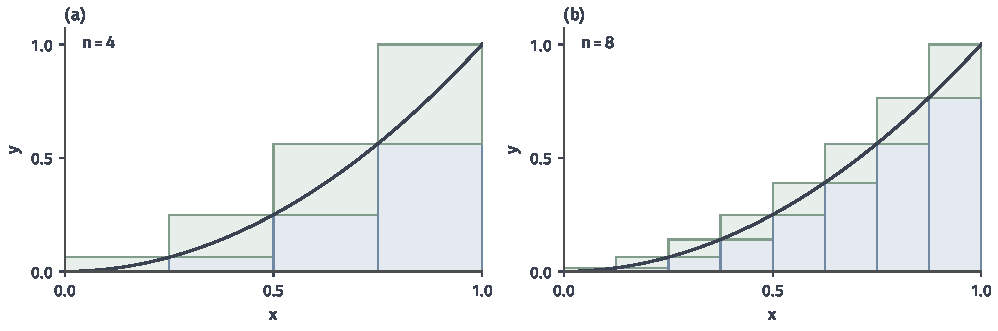
\includegraphics[width=169.0mm]{figures/01-mathematical-preliminaries-upper/01-mathematical-language-combinatorics-analysis-optimization/matplotlib/chapter3-concept-processes/riemann-upper-lower.pdf}
 \caption{对$[0,1]$上的$f(x)=x^2$，分别等分为4段、8段。蓝色矩形累计下和，补上绿色部分得到上和，黑线为函数图像。两种颜色之间的面积差是$U_n-L_n=1/n$，从$1/4$降到$1/8$；Darboux判据要求这种差能任意小，而不只是选定一张图时较小。}
 \label{fig:analysis-process-riemann-upper-lower}
\end{figure*}

\subsubsection{黎曼积分的局限}

连续函数以及只有有限个间断点的有界函数都已证明黎曼可积，但这不能说明任意有界函数都能通过细分区间累计。下面用同一个零测点集构造反例，并说明这与积分在函数极限下的稳定性有什么关系。


\paragraph{狄利克雷函数}
前面的可积条件要求各段振幅乘长度后的总误差趋零。现在考察一个有界函数，说明仅靠继续缩短输入区间，可能始终无法减小这种误差。
令$Q_0=\mathbb Q\cap[0,1]$，$d(x)=\mathbb I_{Q_0}(x)$，称为狄利克雷函数。
每个非退化小区间都含有有理数和无理数，所以任意分割的每段都有$m_i=0$、$M_i=1$，从而
\[
 L(d,P)=0,\qquad U(d,P)=1.
\]
即使分割任意细，全部选有理取样点会得到黎曼和$1$，全部选无理取样点会得到$0$。
这不是取样还不够密，而是“所有细分割与所有取样都给出共同极限”的要求在这里不成立，因此$d$不黎曼可积。

上一节已经证明$m(Q_0)=0$、$m([0,1]\setminus Q_0)=1$。若按这两个取值集合累计，取值$1$只对应零测范围，取值$0$对应其余范围，所需的有限计算便是
\[
 1\cdot m(Q_0)+0\cdot m([0,1]\setminus Q_0)=0.
\]
这提示我们，扩大积分范围可以改变分组依据：不再只用相邻输入的小区间代表函数，而允许把具有同一取值的输入归为一组。

黎曼方法在极限过程中还有同样的范围障碍。列举$Q_0=\{q_1,q_2,\ldots\}$，令$d_n=\mathbb I_{\{q_1,\ldots,q_n\}}$。
每个$d_n$只在有限点非零，黎曼可积且积分为$0$；它们却逐点递增到不黎曼可积的$d$。
所以各步都能积分，并不保证极限仍能用同一定义积分。后面将看到，新的分层累计既能处理$d$，也能在非负单调逼近下保留积分极限。

这并不否定黎曼积分在连续函数等情形中的作用。新的构造还必须证明，在原来黎曼可积的范围内，它与已有积分相等。

\subsection{勒贝格定积分}
\label{sec:analysis-lebesgue-definite-integral}

狄利克雷函数已经给出两个可测取值集合，因而能按“函数值乘相应集合的测度”计算。
一般函数可能取无限多个值，需要先把取值范围分成有限档，再逐步缩小档宽并提高截断高度。
每一档对应的输入集合可能散布在许多位置，不再要求是一个区间。

这时前一节的测量结构分别承担明确任务：$\sigma$代数保证各档集合及其可数运算仍在允许范围内，测度为每档赋予大小。
还缺的条件在函数一侧：由它划出的各档是否可测？这就是先引入可测函数的原因。
保证分层有意义之后，再定义有限档的简单函数积分、非负函数的积分，最后检查有符号累计是否有限。

\subsubsection{可测函数}
\label{sec:analysis-measurable-functions}

按取值分层之前，必须先给函数一个资格条件：这些层在输入端是否属于已选的可测范围。这个条件只负责能否测量，不负责总量是否有限。


\paragraph{可测函数的定义}
可测集是输入范围中的集合，可测函数则要保证：指定输出的一段取值范围后，落入这段范围的输入仍组成可测集。
例如要计算取值大于$c$的输入占多大测度，必须先有$\{x:f(x)>c\}\in\mathcal A$，才能使用$\mu$对它赋值。

一般地，输出范围取Borel集$B\subseteq\mathbb R$，分层累计的对象关系是
\[
 B\longmapsto f^{-1}(B)=\{x\in X:f(x)\in B\}
 \longmapsto\mu(f^{-1}(B)).
\]
这里对输入集合使用$\mu$，没有把函数值本身当成集合的测度。
下面用所有Borel原像可测的要求规定函数的可测性。
\begin{definition}[可测函数]
\label{def:analysis-measurable-function}
设$X\subseteq\mathbb R$，$(X,\mathcal A,\mu)$为测度空间。函数$f:X\to\mathbb R$称为\term{可测函数}（measurable function），若对每个Borel集$B\subseteq\mathbb R$，原像$f^{-1}(B)$都属于$\mathcal A$。等价地，只需对每个$a\in\mathbb R$有$\{x\in X:f(x)>a\}\in\mathcal A$。扩展实轴$[-\infty,+\infty]$的Borel结构由射线$(a,+\infty]$（$a\in\mathbb R$）生成，扩展实值函数按此结构作同样定义。
\end{definition}
阈值条件之所以足够，是因为射线$(a,\infty)$生成实轴的Borel $\sigma$代数，且原像保持补集与可数并。
具体地，所有原像属于$\mathcal A$的输出集合本身构成一个$\sigma$代数；若它包含全部射线，就包含这些射线生成的全部Borel集。
因此，既可以逐个检验阈值集合，也可以直接使用Borel原像条件。

例如一档取值$[u,v)$对应$\{u\leq f<v\}$，它是Borel集$[u,v)$的原像，因而可测。
对于狄利克雷函数，各档的原像只可能是$\varnothing,Q_0,[0,1]\setminus Q_0,[0,1]$，都勒贝格可测。
所以它虽不满足黎曼可积要求，却已经具备新构造所需的分层资格；这还没有替任意函数保证积分有限。
反过来，若$A\subseteq X$不属于$\mathcal A$，示性函数$\mathbb I_A$就不可测，因为$\{\mathbb I_A>1/2\}=A$。
此时连非零取值落在哪个可测范围内都无法满足要求，不能直接套用“取值乘测度”的规则。

可测性还依赖指定的$\sigma$-代数。例如$X=\{0,1\}$上仅取$\mathcal A=\{\varnothing,X\}$，函数$f(0)=0,f(1)=1$不可测，因为$\{f>1/2\}=\{1\}\notin\mathcal A$；若改取幂集$\mathcal P(X)$，同一函数就可测。

\paragraph{连续函数与可测函数}
新的函数范围应包含原来熟悉的连续函数，同时容纳促使我们改变积分构造的狄利克雷函数。
在实轴Borel结构下，连续函数可测，因为开集的原像是开集。若定义域使用包含Borel集的勒贝格可测结构，结论仍成立。反之，可测函数不必连续：狄利克雷函数的两个取值集合都勒贝格可测，所以它可测，却在每一点间断。

\paragraph{可测函数的运算}
分层累计还要用于函数的加减、相乘和复合，因此应先保证这些运算不会把函数带出可测范围。
实值可测函数的和、积、绝对值、最大值与最小值仍可测。以和为例，
\[
 \{f+g>a\}=\bigcup_{q\in\mathbb Q}\bigl(\{f>q\}\cap\{g>a-q\}\bigr),
\]
右侧为可数个可测集合的并。连续实函数与可测函数复合仍可测，因而平方和绝对值可测；再由$fg=((f+g)^2-(f-g)^2)/4$得到乘积可测。最大、最小可由绝对值表达。商在分母不为零的可测集合上可测；若要扩展到全域，需另行指定零点处的可测取值。

对两个一般可测映射，复合还须核对中间可测结构：若$f:(X,\mathcal A)\to(Y,\mathcal B)$和$g:(Y,\mathcal B)\to(Z,\mathcal C)$可测，则$(g\circ f)^{-1}(C)=f^{-1}(g^{-1}(C))\in\mathcal A$。仅说两个实函数各自勒贝格可测，不能跳过中间结构就认定任意复合也可测。扩展实值运算还要排除$\infty-\infty$等未定义形式。

\subsubsection{积分的定义}

测度已经能计算可测集合的大小，现在先把它接到有限取值函数上，再借助下方逼近得到一般非负函数的累计。最后通过正负分解处理带符号取值。


\paragraph{简单函数}
先处理只取有限多个值的可测函数：若它在可测集$E_j$上恒为$a_j$，该组的贡献就应为$a_j\mu(E_j)$。
把各组取为两两不交后，每个输入只计一次，这正是前一节测度有限可加性所支持的累计方式。
下面先对非负取值定义积分，有负取值时稍后再拆成正负两部分。
\begin{definition}[简单函数及其积分]
\label{def:analysis-simple-function-integral}
只取有限个实数值的可测函数称为\term{简单函数}（simple function）。若$s=\sum_{j=1}^m a_j\mathbb I_{E_j}$，其中$a_j\geq0$、$E_j\in\mathcal A$两两不交，则定义
\begin{equation}
 \int_Xs\,\mathrm d\mu=\sum_{j=1}^m a_j\mu(E_j).
\label{eq:analysis-simple-integral}
\end{equation}
这里约定$0\cdot\infty=0$，允许积分为$+\infty$。
\end{definition}
同一简单函数可能有不同表示，需要确认计算不依赖分组方式。
把两种表示的集合用交集作公共细分，每个新块可测且函数值固定；用测度的有限可加性拆开原来的各项，便得到相同的有限和。
同一方法也证明非负简单函数的加法、非负数乘和大小关系都与积分相容。

这个定义把上一节的测度接到了函数累计上。对可测$A$，$\int_X\mathbb I_A\,\mathrm d\mu=\mu(A)$，
说明测量集合就是对它的指示函数积分；对常数$c\geq0$，则有$\int_Xc\,\mathrm d\mu=c\mu(X)$。
特别地，按勒贝格测度累计狄利克雷函数，得到$\int_{[0,1]}d\,\mathrm dm=m(Q_0)=0$。
这里按可测块的大小累计，没有把不可数多个单点的零长度当作一个可数级数相加。

图~\ref{fig:integral-value-layers}用同一函数比较两种分组方式。黎曼和的每个组是相邻输入组成的区间；简单函数的一档则由取值条件确定，输入集合可以分成互相分离的几段。

\begin{figure*}[htbp]
 \centering
 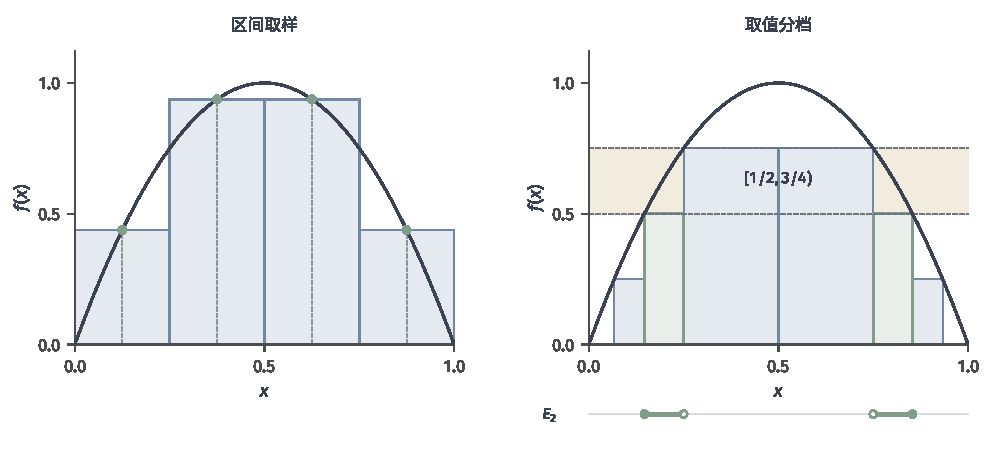
\includegraphics[width=169mm]{figures/01-mathematical-preliminaries-upper/01-mathematical-language-combinatorics-analysis-optimization/matplotlib/integral-value-layers/figure.pdf}
 \caption{对同一函数$f(x)=4x(1-x)$（$0\leq x\leq1$）作有限近似。左侧等分输入区间为四段，在中点取样形成黎曼和，矩形可高于或低于曲线。右侧将输出范围按$1/4$分档，在$E_j=\{x:j/4\leq f(x)<(j+1)/4\}$上取下界$a_j=j/4$；绿色标出$E_2=\{1/2\leq f<3/4\}$对应的两个输入区间，它们的总测度乘$1/2$给这一档的贡献。下方单独画出$E_2$并标明端点。最大值处的单点不影响积分，图中略去。左侧累计为$\sum_i f(\xi_i)\Delta x_i$，右侧简单函数的累计为$\sum_j a_jm(E_j)$。勒贝格构造加细的是取值档，权重仍来自输入集合的测度。}
 \label{fig:integral-value-layers}
\end{figure*}


\paragraph{非负勒贝格积分}
一般非负可测函数未必只取有限多个值，不能直接使用上面的有限和。
我们先保留简单函数：让它们从下方估计$f$，其积分给出能够确定的累计下界，再取全部下界的上确界作为总量。
\begin{definition}[非负勒贝格积分]
\label{def:analysis-nonnegative-lebesgue-integral}
若$f:X\to[0,\infty]$可测，定义
\begin{equation}
 \int_Xf\,\mathrm d\mu
 =\sup\left\{\int_Xs\,\mathrm d\mu:
       s\text{为非负简单函数},\ 0\leq s\leq f\right\}.
\label{eq:analysis-nonnegative-lebesgue-integral}
\end{equation}
这称为$f$关于$\mu$的非负\term{勒贝格积分}（Lebesgue integral），值可为$+\infty$。
\end{definition}
取下方积分的上确界，是为了保留所有简单函数能累计到的贡献，而不依赖某次取样。对可测$A\subseteq X$，记$\int_Af\,\mathrm d\mu=\int_Xf\mathbb I_A\,\mathrm d\mu$。在实轴上对勒贝格测度积分时，常写$\mathrm dx$代替$\mathrm dm(x)$；使用其他测度时写明$\mathrm d\mu$。

例如$f(x)=x$在$[0,1]$上的两段下方阶梯积分为$1/4$，四段时为$3/8$；等分为$n$段时，下方阶梯积分为$(n-1)/(2n)$，上方阶梯积分为$(n+1)/(2n)$，二者都趋于$1/2$。图~\ref{fig:analysis-simple-integral}用$f(x)=x^2$展示相同的逐级逼近。
\begin{figure*}[htbp]
 \centering
 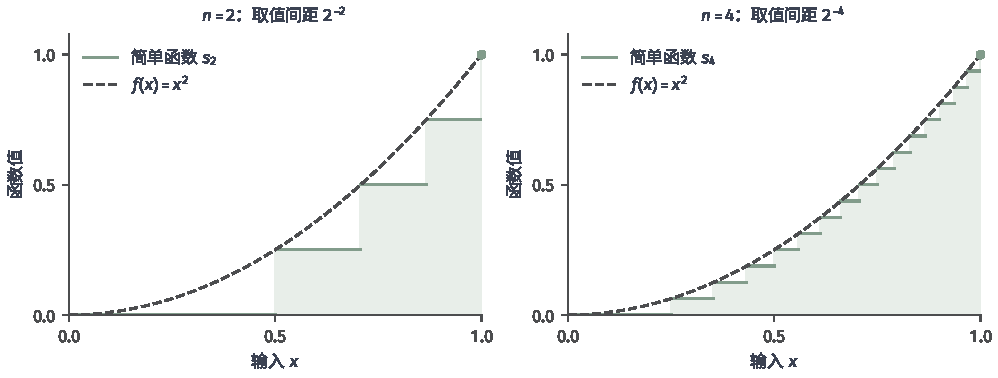
\includegraphics[width=169.0mm]{figures/01-mathematical-preliminaries-upper/01-mathematical-language-combinatorics-analysis-optimization/matplotlib/analysis-simple-integral/figure.pdf}
 \caption{$f(x)=x^2$在$[0,1]$上的简单函数逼近。图中将区间分别等分为两段、四段，在每段取函数下界，按高度乘长度求和；加细后下方累计增大，逼近积分$1/3$。简单函数还允许用一般可测集合代替图中的区间。}
 \label{fig:analysis-simple-integral}
\end{figure*}

\paragraph{可测函数的简单逼近}
上确界定义说明了怎样确定总量，还应给出实际的一列下方近似，解释任意非负可测函数如何由有限分层建立。
只加细网格会留下无穷多个取值，只截断高度又没有消除连续取值，因此同时把高度截断到$n$，再将取值向下舍入到步长$2^{-n}$的网格，得到
\begin{equation}
 \begin{aligned}
 s_n(x)&=\sum_{k=0}^{n2^n-1}\frac{k}{2^n}
  \mathbb I_{\{k/2^n\leq f<(k+1)/2^n\}}(x)\\
 &\quad+n\mathbb I_{\{f\geq n\}}(x).
 \end{aligned}
\label{eq:analysis-canonical-simple-approximation}
\end{equation}
每个$s_n$只取有限个值，取值集合可测，且$0\leq s_n\leq f$。从$n$到$n+1$时网格加细、截断高度增大，所以下方近似不减。有限$f(x)$最终低于截断高度，舍入误差小于$2^{-n}$；$f(x)=\infty$时$s_n(x)=n$。因此$s_n\uparrow f$逐点成立。这里先建立函数逼近，积分极限等式将在单调收敛定理中证明。

\paragraph{有符号勒贝格积分}
非负函数只有增加贡献的问题；有正负值时，还必须防止把两个无穷总量相减。
对实值可测$f$，令$f^+=\max\{f,0\}$、$f^-=\max\{-f,0\}$，则$f=f^+-f^-$、$|f|=f^++f^-$，正负两部分均非负可测。
只要它们的积分不同时为无穷，就定义
\[
 \int_Xf\,\mathrm d\mu=\int_Xf^+\,\mathrm d\mu-\int_Xf^-\,\mathrm d\mu.
\]
这允许单个无穷值；若两部分都为无穷，差没有定义，不能通过选择某种抵消次序给它指定一个有限勒贝格积分。

\subsubsection{可积性的要求}

可测性保证取值层可以测量；非负积分的定义保证有一个确定的扩展实数值，但都没有保证累计有限。
若要使有符号积分成为有限实数，就必须让正负两部分的总量都有限，下面用等价的绝对值积分条件统一规定。

\begin{definition}[勒贝格可积函数]
\label{def:analysis-integrable-function}
若实值可测$f$满足
\begin{equation}
 \int_X|f|\,\mathrm d\mu<\infty,
\label{eq:analysis-absolute-integrability}
\end{equation}
则称$f$关于$\mu$勒贝格可积，也称\term{绝对可积}（absolutely integrable）。其有符号勒贝格积分是有限实数。
\end{definition}
由于$f^+,f^-\leq|f|$，下方简单函数的比较保证二者的积分有限，所以这一定义确实给出有限的有符号积分。本节未附“黎曼”或“反常”限定的可积性均指这一绝对可积条件。

\paragraph{有限积分的条件}
下面分开检查“积分已经定义”和“积分取有限值”，并说明有界性还需与输入范围的测度一起判断。
非负可测函数总有定义好的非负勒贝格积分，但这个值未必有限。对有符号函数，有限积分要求正负部分都具有有限积分，等价于式~\eqref{eq:analysis-absolute-integrability}；这一等价性将在下一小节由非负积分加法正式证明。有限的有符号勒贝格积分因而必然绝对可积，不存在以正负无穷抵消得到的有限值。

若$\mu(X)<\infty$且$|f|\leq M$，由积分定义的比较关系可得$\int_X|f|\,\mathrm d\mu\leq M\mu(X)<\infty$，所以有界可测函数可积。无穷测度范围上，有界性不足，例如实轴上的常数一。无界也未必不可积，反常积分小节将算出$x^{-1/2}$在$(0,1)$上的有限积分。

\paragraph{积分与平均值}
积分不仅取决于函数和输入范围，还取决于用什么测度赋予各部分大小。
沿用前面有限加权累计的思路，取$X=\{0,1\}\subseteq\mathbb R$，设$\mu(\{0\})=1$、$\mu(\{1\})=2$，$f(0)=3$、$f(1)=-1$，则$\int_Xf\,\mathrm d\mu=1$而$\int_X|f|\,\mathrm d\mu=5$。只有在$0<\mu(X)<\infty$且$f$可积时，才能进一步定义平均值$\mu(X)^{-1}\int_Xf\,\mathrm d\mu$，本例为$1/3$。总质量为一的概率测度无需再归一化。
若同一个$X$改用勒贝格测度，两个点的长度均为零，上述函数的积分就变为零。
这与按权重$1,2$得到的$1$不矛盾，而是说明更换测度就更换了累计规则；此时总测度也为零，不能再用前面的除法定义平均值。

\subsubsection{积分的性质}
\label{sec:analysis-lebesgue-basic-properties}

定义已经给出累计值，现在要检查它是否保持加法、大小关系与集合分拆。
先从简单函数和上确界证明非负情形，再用正负分解处理有限的有符号积分；以下均指关于指定测度$\mu$的勒贝格积分。

\paragraph{非负积分的基本性质}
简单函数的积分具有线性与单调性，现在从上确界定义把这些性质推广到一般非负可测函数。证明只用前面建立的集合测度性质，为后面的累计函数和微积分基本定理提供依据。
\begin{theorem}[非负勒贝格积分的线性与单调性]
\label{lem:analysis-nonnegative-integral-properties}
设$(X,\mathcal A,\mu)$为测度空间，$f,g:X\to[0,\infty]$可测，$\alpha,\beta$为非负实数。
若$f\leq g$几乎处处，则$\int_Xf\,\mathrm d\mu\leq\int_Xg\,\mathrm d\mu$；
在$0\cdot\infty=0$的约定下，还有
\[
 \int_X(\alpha f+\beta g)\,\mathrm d\mu
 =\alpha\int_Xf\,\mathrm d\mu+\beta\int_Xg\,\mathrm d\mu.
\]
若$f=g$几乎处处且两者均可测，则它们的非负积分相同。
\end{theorem}
\begin{proof}
逐点单调性直接来自定义：每个简单函数$0\leq s\leq f$也满足$s\leq g$。
若$N$可测且$\mu(N)=0$，简单函数在$N$上的积分为零。
对$f,g$在$X\setminus N$相等的情形，将任意$0\leq s\leq f$在$N$上置零，
所得简单函数不超过$g$且积分未变。取上确界得$\int f\leq\int g$，反向相同；
几乎处处的单调性也可先作这项可测零集修改。这里不在未完备空间中任意改动后省略可测性。

对加法，任取非负简单函数$s\leq f$、$t\leq g$，简单函数的有限线性给出
$\int(f+g)\geq\int s+\int t$。分别取上确界，得到
$\int(f+g)\geq\int f+\int g$。若右侧为无穷，这已给出等式；以下设右侧有限。
反向需要检查每个下方简单函数的累计。取任意非负简单函数
$u=\sum_{j=1}^m a_j\mathbb I_{E_j}\leq f+g$，其中$a_j>0$、$E_j$两两不交，
并取规范简单逼近$s_n\uparrow f$、$t_n\uparrow g$。
固定$c\in(0,1)$，令$E_{j,n}=E_j\cap\{s_n+t_n\geq ca_j\}$。
因$s_n+t_n\uparrow f+g$且$f+g\geq a_j$于$E_j$，有$E_{j,n}\uparrow E_j$。
第~\ref{sec:analysis-set-measure-continuity}节的测度递增连续性及简单函数线性给出
\[
 \begin{aligned}
 c\int_Xu\,\mathrm d\mu
 &=\lim_n c\sum_j a_j\mu(E_{j,n})\\
 &\leq\liminf_n\left(\int_Xs_n\,\mathrm d\mu+\int_Xt_n\,\mathrm d\mu\right)\\
 &\leq\int_Xf\,\mathrm d\mu+\int_Xg\,\mathrm d\mu.
 \end{aligned}
\]
先令$c\uparrow1$，再对所有这样的$u$取上确界，便得到反向不等式。
正数倍的结论由$s\leq\alpha f$与$s/\alpha\leq f$在定义中的一一对应推出；
零数倍按约定处理，再与加法结合即得一般结论。
整个证明只使用简单函数有限和、积分上确界与集合测度连续性，没有使用一般函数的单调收敛定理。
\end{proof}

\paragraph{有符号勒贝格积分的性质}
有正负值时，实线性需要先保证所有参与相减的总量有限；绝对可积性正是这一要求。
下面同时证明可积性判别、有限线性、比较与绝对值估计。
\begin{theorem}[有符号勒贝格积分的基本性质]
\label{thm:analysis-signed-integral-properties}
设$(X,\mathcal A,\mu)$为测度空间，$f,g:X\to\mathbb R$可测。
函数$f$勒贝格可积，当且仅当$\int f^+\,\mathrm d\mu$与$\int f^-\,\mathrm d\mu$都有限。
若$f,g$勒贝格可积，$\alpha,\beta\in\mathbb R$，则$\alpha f+\beta g$也可积，且
\[
 \int_X(\alpha f+\beta g)\,\mathrm d\mu
 =\alpha\int_Xf\,\mathrm d\mu+\beta\int_Xg\,\mathrm d\mu.
\]
对上述可积的$f,g$，$f\leq g$几乎处处时有$\int f\leq\int g$，并且
\[
 \left|\int_Xf\,\mathrm d\mu\right|\leq\int_X|f|\,\mathrm d\mu.
\]
若$f$可积、$g=f$几乎处处且$g$可测，则$g$也可积，积分与$f$相同。
\end{theorem}
\begin{proof}
由$|f|=f^++f^-$及非负积分加法，
$\int|f|=\int f^++\int f^-$，所以绝对积分有限等价于正负两项均有限。
先检查有符号积分与正负分解以外的表示是否相容。若$f=u-v$，其中$u,v$非负且可积，
则$f^+,f^-\leq u+v$，故$f$可积；非负恒等式$u+f^-=v+f^+$积分后可移去有限项，得到
$\int f=\int u-\int v$。

对可积$f,g$，$|f+g|\leq|f|+|g|$保证和可积。
将$f+g=(f^++g^+)-(f^-+g^-)$代入刚才的分解结论，再用非负加法，得到
$\int(f+g)=\int f+\int g$。正数倍沿用非负缩放，负数倍交换正负部分，零数倍直接成立，因而实线性成立。
若$f\leq g$几乎处处，可积差$g-f$的积分非负，移项即得比较关系。
定义中的正负分解与实数三角不等式给出
$|\int f|\leq\int f^++\int f^-=\int|f|$。
最后，若$f=g$几乎处处且均可测，非负积分的零测修改不变性分别用于$|f|,|g|$及正负部分，便得$g$可积且积分相同。
\end{proof}

这里没有通过正负无穷抵消得到有限值。非负积分可以等于无穷，但有符号线性中的任意移项必须满足上述有限性条件。

\paragraph{零积分与零测例外}
非负函数没有正负抵消，积分为零应表示它的正值只落在零测范围内。
下面把这一判断写成等价条件，供后面比较两种积分时使用。
\begin{theorem}[非负函数的零积分判别]
\label{thm:analysis-zero-integral}
设$(X,\mathcal A,\mu)$为测度空间，$f:X\to[0,\infty]$可测，则
\[
 \int_Xf\,\mathrm d\mu=0\quad\Longleftrightarrow\quad f=0\ \text{几乎处处}.
\]
特别地，实值可测$f$满足$\int|f|\,\mathrm d\mu=0$当且仅当$f=0$几乎处处。
\end{theorem}
\begin{proof}
若积分为零，对每个正整数$k$，$f\geq k^{-1}\mathbb I_{\{f\geq1/k\}}$，故
$0\geq k^{-1}\mu(\{f\geq1/k\})$。这些集合都零测，而
$\{f>0\}=\bigcup_{k\geq1}\{f\geq1/k\}$，所以$f=0$几乎处处。
反之，非负积分的零测修改不变性将$f$与零函数的积分相等。将结论用于$|f|$便得最后一条。
\end{proof}
对有正负值的$f$，仅有$\int f=0$不能推出$f=0$几乎处处，例如$f(x)=x$在$[-1,1]$上的积分为零。

\paragraph{积分范围的可加性}
函数值可以相加，积分范围也可以分拆；后者要保持的是可测集合的不交并。
下面从测度的可数可加性直接证明这一性质，不提前使用函数列的收敛定理。
\begin{theorem}[勒贝格积分的区域可加性]
\label{thm:analysis-integral-set-additivity}
设$(X,\mathcal A,\mu)$为测度空间，$A_n\in\mathcal A$两两不交，$A=\bigcup_{n\geq1}A_n$。
若$f:X\to[0,\infty]$可测，则
\[
 \int_Af\,\mathrm d\mu=\sum_{n=1}^{\infty}\int_{A_n}f\,\mathrm d\mu,
\]
允许等式两侧为无穷。若$f$实值且在$A$上绝对可积，同一等式成立，且右侧绝对收敛。
对可测$B,C$及在$B\cup C$上绝对可积的实值$f$，还有
\[
 \int_{B\cup C}f=\int_Bf+\int_Cf-\int_{B\cap C}f.
\]
特别地，$C\subseteq B$时有$\int_{B\setminus C}f=\int_Bf-\int_Cf$。
\end{theorem}
\begin{proof}
非负积分的有限区域加法来自示性函数恒等式与非负线性。
因此$\int_A f\geq\sum_{n=1}^N\int_{A_n}f$对每个$N$成立，取部分和的上确界得到一个方向。
反向取任意简单函数$0\leq s=\sum_{j=1}^r c_j\mathbb I_{E_j}\leq f\mathbb I_A$，其中$c_j>0$且$E_j$两两不交、均包含于$A$。
测度的可数可加性及有限和与非负级数的合并给出
\[
 \int_Xs\,\mathrm d\mu
 =\sum_{j=1}^r c_j\sum_{n\geq1}\mu(E_j\cap A_n)
 =\sum_{n\geq1}\int_{A_n}s\,\mathrm d\mu
 \leq\sum_{n\geq1}\int_{A_n}f\,\mathrm d\mu.
\]
对全部这样的$s$取上确界，得到反向不等式。

若$f$在$A$上绝对可积，先对$|f|$使用非负结论，得到
$\sum_n|\int_{A_n}f|\leq\sum_n\int_{A_n}|f|=\int_A|f|<\infty$。
再分别对$f^+,f^-$使用等式并相减，便得到有符号版本。
最后，将有限实线性用于
$\mathbb I_{B\cup C}+\mathbb I_{B\cap C}=\mathbb I_B+\mathbb I_C$即得容斥式，包含情形再化为差集式。
\end{proof}
非负无穷积分的区域相加仍成立，但不能把它任意改写为含$\infty-\infty$的差。

\subsubsection{与黎曼积分的关系}

新的定义既要处理原来无法累计的函数，也要与已有数值相容。下面先证明黎曼可积函数没有被改变，再说明零测改值为什么使两种可积范围分开。


\paragraph{黎曼积分与勒贝格积分的关系}
改变累计方式之后，必须检验原来已经能够计算的积分是否得到保留。
下面将黎曼上下和看作简单函数的积分，以可测包络和零测余量证明两种积分一致。
\begin{theorem}[黎曼积分与勒贝格积分的一致性]
\label{thm:analysis-riemann-lebesgue-consistency}
设$a<b$，$f:[a,b]\to\mathbb R$有界且黎曼可积。
则$f$勒贝格可测、勒贝格可积，且
\[
 \int_a^bf(x)\,\mathrm dx\ \text{（黎曼）}
 =\int_{[a,b]}f\,\mathrm dm\ \text{（勒贝格）}.
\]
反向蕴含不成立：有界勒贝格可积函数未必黎曼可积。
\end{theorem}
\begin{proof}
设$|f|\leq M$在$[a,b]$上黎曼可积。由Darboux判据，可取一列分割$P_n$，后一个是前一个的加细，并使$U(f,P_n)-L(f,P_n)<1/n$。
在$P_n$的每个小区间内部，令下阶梯函数$\ell_n$取该段的下确界$m_i$，上阶梯函数$u_n$取上确界$M_i$；
有限个分割点上的取值不影响积分，可以都取$f$的值。于是$\ell_n\leq f\leq u_n$，它们都是简单函数，
且$\int\ell_n\,\mathrm dx=L(f,P_n)$、$\int u_n\,\mathrm dx=U(f,P_n)$。加细使$\ell_n$逐点不减、$u_n$逐点不增。
令$\ell=\sup_n\ell_n$、$u=\inf_nu_n$。它们可测，因为$\{\ell>c\}=\bigcup_n\{\ell_n>c\}$是可数个可测集合的并，$u$同理；并且$\ell\leq f\leq u$。
非负可测函数$u-\ell$对每个$n$都满足$u-\ell\leq u_n-\ell_n$，由积分的单调性，
\[
 0\leq\int_{[a,b]}(u-\ell)\,\mathrm dx\leq U(f,P_n)-L(f,P_n)<\frac1n,
\]
所以这个积分为零。由定理~\ref{thm:analysis-zero-integral}，$\{u\neq\ell\}$是零测集。$f$只在这个零测集上可能与可测函数$\ell$不同，
而勒贝格测度完备，零测集的任意子集都可测，所以$f$勒贝格可测。有限区间上的有界可测函数绝对可积，故可使用有符号积分的比较关系。
最后，每个$n$都有$L(f,P_n)=\int\ell_n\leq\int f\leq\int u_n=U(f,P_n)$（有符号情形先给$f$加常数$M$使之非负，再用有限线性移去常数），
两端都趋于黎曼积分，所以勒贝格积分等于黎曼积分。

狄利克雷函数是有界勒贝格可积却不黎曼可积的反例，证明了反向蕴含不成立。
\end{proof}

\paragraph{黎曼可积性的测度判据}
一致性定理保留了已有积分，却还没有回答哪些勒贝格可积函数同时黎曼可积。
下面将上下和误差与不连续点的测度联系起来，给出有界函数的准确判据。
\begin{theorem}[黎曼可积性的勒贝格判据]
\label{thm:analysis-riemann-lebesgue-criterion}
设$a<b$，$f:[a,b]\to\mathbb R$有界，$D$为$f$相对于$[a,b]$的不连续点集。
则$D$勒贝格可测，并且$f$黎曼可积当且仅当$m(D)=0$。
\end{theorem}
\begin{proof}
先用局部振幅描述不连续。记$I_r(x)=[a,b]\cap(x-r,x+r)$，定义
\[
 \omega_f(x)=\inf_{r>0}\left(\sup_{I_r(x)}f-\inf_{I_r(x)}f\right).
\]
由于$x\in I_r(x)$，$\omega_f(x)=0$恰好表示在足够小的邻域内所有取值都接近$f(x)$，因此等价于$f$在$x$连续。
对$t>0$，记$D_t=\{x:\omega_f(x)\geq t\}$。
若$\omega_f(x)<t$，存在一个邻域，其上振幅小于$t$；该邻域内充分靠近$x$的点也有更小的邻域包含于其中，所以也不属于$D_t$。
因此$D_t$在$[a,b]$中闭，进而紧；$D=\bigcup_{k\geq1}D_{1/k}$为Borel集。

若$f$黎曼可积，给定$t,\varepsilon>0$，取分割$P$使$U(f,P)-L(f,P)<t\varepsilon$。
除有限个分割点外，$D_t$中的每点都位于某个振幅至少为$t$的小区间内。
这些小区间的总长度不超过$(U-L)/t<\varepsilon$，分割点自身零测，故$m(D_t)<\varepsilon$。
由$\varepsilon$任意得$m(D_t)=0$，再取可数并得到$m(D)=0$。

反之，设$m(D)=0$且$|f|\leq M$；$M=0$时结论直接成立，以下取$M>0$。
给定$\varepsilon>0$，先取$t>0$使$t(b-a)<\varepsilon/2$。
紧零测集$D_t$可由开集$O$包住，使$m(O)<\varepsilon/(4M)$。
每个$x\notin D_t$都有一个相对开邻域$V_x$，其上$f$的振幅小于$t$。
$O$与这些$V_x$覆盖$[a,b]$，取一个有限子覆盖。
由式~\eqref{eq:analysis-cover-uniform-radius}，这个覆盖存在共同半径$r>0$，使每点的相对$r$球包含在某个覆盖成员内。取$\delta=r$，长度小于$\delta$的子区间就落在以其中一点为中心的$r$球内，因此也落在某个覆盖成员内。

取细度小于$\delta$的分割。能落在某个$V_x$内的小区间，振幅小于$t$；其余小区间都包含于$O$，总长度不超过$m(O)$，振幅至多$2M$。
因此
\[
 U(f,P)-L(f,P)\leq t(b-a)+2M m(O)<\varepsilon.
\]
由Darboux判据，$f$黎曼可积。
\end{proof}

\paragraph{零测集上的改值}
前面的累计按可测块的测度赋权，因而只落在可测零测集上的贡献为零。
保持可测性的零测修改不改变勒贝格积分，这已在定理~\ref{lem:analysis-nonnegative-integral-properties}及定理~\ref{thm:analysis-signed-integral-properties}中证明。这里用它比较两种可积范围，而不再从简单函数重新推导。
在勒贝格测度下，完备性保证任意零测子集仍可测，所以零测范围内任意有限实值改动都保持可测性。
若采用未完备的一般测度空间，则不能省略修改后仍可测的条件。
狄利克雷函数与零函数的关系正是这个机制的实例。

这种修改可能破坏黎曼可积性。零函数在可数稠密集$\mathbb Q\cap[0,1]$上改为一，就变为不黎曼可积的狄利克雷函数。因此黎曼可积性判据要求原函数几乎处处连续，不能替换成“几乎处处等于一个连续函数”。有限个点的有限改值仍保持黎曼可积，修改前后的积分才仍相等。

\subsection{不定积分和变上限积分}
\label{sec:analysis-definite-indefinite-integrals}

定积分在指定范围上给出一个数；寻找导数等于给定函数的原函数，则产生一个函数族。把定积分的上端点设为变量也会得到一个函数，下面先分别定义这两种对象，暂不把它们认定为同一对象。

\subsubsection{不定积分}

这里暂时从累计转回求导问题：给定$f$，寻找导数为$f$的函数。先独立定义这个对象，才能在基本定理中真正证明它与积分的联系。


\paragraph{原函数}
对已知$f$寻找满足$G'=f$的可微函数$G$，称为求原函数。原函数的定义只涉及求导，还没有断言它与定积分有何关系。例如$x^2/2$是$x$在实轴上的一个原函数。

\paragraph{不定积分}
若$f$在区间$I$上有一个原函数$G$，则其全部原函数写为$G+C$，其中$C$为任意实常数，记作$\int f(x)\,\mathrm dx=G(x)+C$，称为不定积分。两个原函数之差的导数为零，由中值定理，它们在区间上只差常数；如果定义域由分离的区间组成，每段可以有不同常数。不定积分表示一个函数族，区别于固定上下限后得到的数值。

\subsubsection{变上限积分}

将固定范围上的积分改为随端点变化的累计，可以得到一个新函数；它的存在来自各子区间可积，尚不等于它已经是原函数。


\paragraph{变上限积分}
若$f$在$[a,b]$上黎曼可积，令
\[
 F(x)=\int_a^xf(t)\,\mathrm dt,\qquad a\leq x\leq b.
\]
得到的$F$称为变上限积分函数，也称累计函数。$t$是积分变量，$x$是函数的自变量。比如$f(t)=1$时，$F(x)=x-a$。变上限积分是否可导、是否以$f$为导数，需要由微积分基本定理判断，不能直接从记号得出。

\paragraph{变上限勒贝格积分}
若$f$在$[a,b]$上勒贝格可积，同样定义$F(x)=\int_a^xf(t)\,\mathrm dt$，此时积分按勒贝格定义计算。可积性保证每个子区间上的积分有限，前面的区域分拆给出$F(y)-F(x)=\int_x^yf$；有界黎曼可积函数的两种累计函数相同。对一般可积函数，累计函数是否处处或几乎处处可导，需要另外证明。

\subsubsection{原函数与累计函数的关系}

原函数从求导关系定义，累计函数从定积分构造；记号相似没有证明二者等价。若$f$连续，下一小节将证明累计函数是它的原函数；若$f$仅勒贝格可积，能一般地保证的是几乎处处恢复$f$。例如阶跃函数可以累计，却不可能在跳跃点附近处处等于某个函数的导数，这一差别将在基本定理中具体检验。

\subsection{微积分基本定理}
\label{sec:measurable-differentiation-recovery}
\label{sec:analysis-fundamental-calculus}

求导记录局部变化，积分记录一段范围内的累计，二者能否相互恢复要分别回答两个问题。
第一，给定函数$G$，积分其导数能否得到$G(b)-G(a)$；第二，给定被积函数$f$，对累计函数$F(x)=\int_a^xf$求导能否恢复$f(x)$。
前者检查总变化是否全部由导数记录，后者检查局部平均是否能识别点值。下面分别说明黎曼与勒贝格条件，不将“处处”与“几乎处处”的结论混在一起。

\subsubsection{导数的积分}

先给定$G$再计算其导数的积分，目标是恢复端点变化。
连续导数提供最直接的充分条件；导数仅黎曼可积时仍可恢复，而只知道几乎处处可导且导数勒贝格可积，还需要对$G$的整体变化加条件。

\paragraph{黎曼可积导数的基本定理}
中值定理把每段端点增量写成导数取样值乘区间长度，因此端点恢复的关键是这些取样和能否趋于积分，而不必要求导数连续。
下面先给出黎曼可积导数的结论；连续导数是其中自动满足可积性的特例。
\begin{theorem}[黎曼可积导数的端点公式]
\label{thm:analysis-riemann-derivative-ftc}
\label{thm:analysis-newton-leibniz-continuous}
设$G$在$[a,b]$上连续、在$(a,b)$上可导，且存在黎曼可积函数$g:[a,b]\to\mathbb R$在内点满足$g=G'$。
则
\[
 \int_a^bg(x)\,\mathrm dx=G(b)-G(a).
\]
端点处给$g$指定的有限值不影响积分。特别地，若$G\in C^1([a,b])$，可取$g=G'$。
上述黎曼积分也等于相应的勒贝格积分。
\end{theorem}
\begin{proof}
对任意分割，在每个小区间上用中值定理选$\xi_i$，得到
\[
 G(b)-G(a)=\sum_i\bigl(G(x_i)-G(x_{i-1})\bigr)
 =\sum_i g(\xi_i)(x_i-x_{i-1}).
\]
$g$黎曼可积保证任意细分割的这些取样和都趋于$\int_a^bg$，所以等式成立。
改变两个端点的值仍保持黎曼可积且不改变积分。若$G\in C^1([a,b])$，连续函数的黎曼可积性保证可选$g=G'$；两种积分的一致性由定理~\ref{thm:analysis-riemann-lebesgue-consistency}给出。
\end{proof}

\paragraph{康托尔函数}
\label{sec:analysis-cantor-function}
几乎处处可导只记录了零测例外之外的局部变化，未必记录全部端点变化。下面的函数连续且几乎处处导数为零，但从$0$到$1$仍增加了$1$。

第~\ref{sec:analysis-cantor-set}节已构造康托尔集$C$并证明它为零测集。现在利用同一删除过程定义一个函数：每一步位于左、右保留区间，分别确定三进制表示的下一位为$0$、$2$，所以$C$中每点都能选只含这两个数字的表示
\[
 x=\sum_{j=1}^\infty\frac{\varepsilon_j}{3^j},\qquad
 F(x)=\sum_{j=1}^\infty\frac{\varepsilon_j/2}{2^j},
 \qquad\varepsilon_j\in\{0,2\}.
\]
第二个几何控制的级数把三进制数字$0,2$分别改为二进制数字$0,1$；$x=1$取全为$2$的表示。若$C$中两点的三进制位首次在第$k$位不同，较大点的二进制主位增加$2^{-k}$，而后续位造成的反向差至多为$\sum_{j>k}2^{-j}=2^{-k}$，所以$F$不减。每个删去区间的两端分别对应某一二进制位为$0$而后全为$1$、该位为$1$而后全为$0$，这条尾和恒等式又保证两值相等。例如$1/3=0.0222\ldots_3$与$2/3=0.2000\ldots_3$都对应$1/2$。在该开区间上把$F$定义为这个共同值，就得到整个$[0,1]$上的\term{康托尔函数}（Cantor function）。

这个函数非减，$F(0)=0,F(1)=1$。在第$n$步的每个保留区间上，它的全部变化不超过$2^{-n}$；删去区间上则不变化。两个相距小于$3^{-n}$的点之间至多涉及两个第$n$步保留区间，因而函数值之差不超过$2^{1-n}$；先选$n$再取输入误差$\delta=3^{-n}$，就得到一致连续性。每个删去的开区间内$F$恒定，所以$F'=0$于$[0,1]\setminus C$，即几乎处处成立；在导数未定义的零测例外上置零，则
\[
 F(1)-F(0)=1,\qquad \int_0^1F'(x)\,\mathrm dx=0.
\]
它不绝对连续：第$n$步保留区间总长度为$(2/3)^n$，但各区间端点变化的总和仍为$2^n2^{-n}=1$。这既解释了绝对连续假设的作用，也说明“连续、几乎处处可导、导数可积”三项合在一起仍不足以由导数积分恢复函数。

\paragraph{绝对连续函数的导数基本定理}
康托尔函数说明，连续性不能排除集中在零测集上的整体变化，因而需要更强的条件。
定义~\ref{def:measurable-absolutely-continuous-function}的绝对连续条件控制许多短区间上的总变化，能排除导数遗漏整体变化的情形。
\begin{theorem}[绝对连续函数的导数积分]
\label{thm:measurable-absolute-continuity-ftc}
若$G:[a,b]\to\mathbb R$绝对连续，则$G'$几乎处处存在，并有实值勒贝格可积函数$g$与$G'$几乎处处相等，使每个$x\in[a,b]$满足
\begin{equation}
 G(x)=G(a)+\int_a^xg(t)\,\mathrm dt.
\label{eq:measurable-absolute-continuity-representation}
\end{equation}
特别地，$G(b)-G(a)=\int_a^bG'(t)\,\mathrm dt$，其中在未定义导数的零测例外上可取值零；这些积分为勒贝格积分。
\end{theorem}
绝对连续性推出几乎处处可导和上述积分表示，是这里引用的测度论基本结论，完整证明见教材\scite{math-folland1999real}。
这项引用包括导数的存在、可积性与端点恢复，不能用已经知道导数存在来代替。
另一个方向——勒贝格可积函数的累计必绝对连续——将在“积分的导数”中直接证明，因此两种描述的等价性仍会建立。

\paragraph{局部Lipschitz连续函数的导数基本定理}
如果用Lipschitz条件控制函数的变化，就能通过绝对连续性保证几乎处处导数存在，并在闭区间上由导数积分恢复总变化。\term{Rademacher定理}（Rademacher theorem）保证例外点只占零测集。
\begin{theorem}[一维Rademacher定理]
\label{thm:measurable-rademacher}
若$U\subseteq\mathbb R$为开集，$f:U\to\mathbb R$局部Lipschitz连续，则$f'$在$U$内几乎处处存在且有限。若$f$在某个开区间上具有Lipschitz常数$L$，则该区间内导数存在的点满足$|f'|\leq L$。
\end{theorem}
这里的导数存在性将通过绝对连续函数基本定理得到，还需用可数覆盖把局部结论合并到整个开集。
\label{sec:analysis-rademacher-proof}
\begin{proof}
紧区间上的Lipschitz函数绝对连续，基本定理便保证它几乎处处可导。若$f$只在开集$U$上局部Lipschitz，可选取可数多个端点为有理数的闭区间，使其内部覆盖$U$，并使每个区间都包含在某个具有Lipschitz常数的邻域内。
各区间上的不可导点集为零测集，它们的可数并仍为零测集，故$f'$在$U$内几乎处处存在。导数存在的点处，Lipschitz差商界取极限便给出$|f'|\leq L$。
\end{proof}
绝对值函数在原点的左右导数不同，仍符合上述几乎处处结论；定理没有把尖点处的左右导数合成一个经典导数。

在闭区间上具有Lipschitz常数的函数绝对连续，因此其导数除几乎处处存在之外，还可用勒贝格积分恢复端点变化。
连续、几乎处处可导、导数可积三项合在一起则不充分，康托尔函数已给出反例。

\subsubsection{积分的导数}

现在改为先给定$f$，再构造累计函数$F(x)=\int_a^xf(t)\,\mathrm dt$。
差商是一个短区间上的平均。下面按被积函数的条件区分三种情况：黎曼可积时先在连续点恢复，局部勒贝格可积时在几乎每一点恢复，闭区间上勒贝格可积时还得到整个区间上的绝对连续性。

\paragraph{黎曼可积函数}
累计函数的增量来自一个短区间，把它除以区间长度后，能否恢复点值取决于该点附近的取值变化。
下面只在要恢复的点要求连续，不额外要求全区间连续。
\begin{theorem}[黎曼累计函数在连续点的导数]
\label{thm:analysis-riemann-primitive-derivative}
设$f$在$[a,b]$上黎曼可积，$F(x)=\int_a^xf(t)\,\mathrm dt$。
若$f$在$c\in(a,b)$处连续，则$F'(c)=f(c)$；端点连续时对应单侧导数也等于端点值。
特别地，若$f$在$[a,b]$上连续，则$F\in C^1([a,b])$且$F'=f$。
\end{theorem}
\begin{proof}
由区间可加性与有限线性，对非零小增量$h$有
\[
 \frac{F(c+h)-F(c)}h-f(c)
 =\frac1h\int_c^{c+h}(f(t)-f(c))\,\mathrm dt.
\]
右侧绝对值不超过$c$与$c+h$之间的$\sup|f(t)-f(c)|$，连续性使它趋零。
对端点只取允许方向的$h$。若$f$处处连续，则所得导数$f$也连续，即$F\in C^1([a,b])$。
\end{proof}

由黎曼可积性的测度判据，不连续点组成零测集，因此这里也得到$F'=f$几乎处处。不能将结论加强为处处成立：阶跃函数$\mathbb I\{x\geq0\}$的累计函数在跳跃点不可导。

\paragraph{局部勒贝格可积函数}
研究某一点附近的平均累计，只需要附近紧范围上的绝对积分有限，不必要求整个定义域的积分有限。
若可测函数$f$在实轴开集$U$内的每个紧子集$K$上都满足$\int_K|f|\,\mathrm dx<\infty$，称$f$局部勒贝格可积。它只要求局部范围内绝对可积，允许整个无界定义域上的绝对积分为无穷。

连续点处的短区间平均趋于函数值。对局部可积函数，\term{Lebesgue微分定理}（Lebesgue differentiation theorem）将这一结论推广到几乎每一点\scite{math-hunter2011measure}。
\begin{theorem}[一维Lebesgue微分定理]
\label{thm:measurable-lebesgue-differentiation}
若$f$在开集$U\subseteq\mathbb R$上局部勒贝格可积，则对几乎每个$x\in U$，
\begin{equation}
 \lim_{r\downarrow0}\frac1{2r}\int_{x-r}^{x+r}|f(t)-f(x)|\,\mathrm dt=0.
\label{eq:measurable-lebesgue-point}
\end{equation}
从而$(2r)^{-1}\int_{x-r}^{x+r}f(t)\,\mathrm dt\to f(x)$。
\end{theorem}
满足式~\eqref{eq:measurable-lebesgue-point}的点称为勒贝格点；定理中的积分均为勒贝格积分。第二条由平均差的绝对值不超过平均绝对差得到。第一条的一般证明需要覆盖估计，本节引用其结论，不把连续点的证明充当一般证明。


在$U$中的一个开区间$I$上固定$x_0\in I$，令$F(x)=\int_{x_0}^xf(t)\,\mathrm dt$。
任意$x\in I$与$x_0$之间的闭区间都是$U$的紧子集，所以积分有限；这里下限不必取在定义域端点。
在$f$的内点勒贝格点$x$，区间可加性给出
\[
 \begin{aligned}
 \left|\frac{F(x+h)-F(x)}h-f(x)\right|
 &\leq\frac1{|h|}\int_{\min\{x,x+h\}}^{\max\{x,x+h\}}|f(t)-f(x)|\,\mathrm dt\\
 &\leq\frac1{|h|}\int_{x-|h|}^{x+|h|}|f(t)-f(x)|\,\mathrm dt.
 \end{aligned}
\]
最后一项是式~\eqref{eq:measurable-lebesgue-point}中平均绝对差的两倍，因而趋零。
所以$F'(x)=f(x)$在每个勒贝格点成立，特别地在$I$上几乎处处成立。
局部可积不能保证靠近定义域端点的累计有限：例如$f(t)=1/t$在$(0,1)$上局部可积，$\int_{1/2}^xf(t)\,\mathrm dt$对每个$x\in(0,1)$有意义，但不能把下限改为$0$而仍要求有限。


\paragraph{勒贝格可积函数}
若进一步要求$f$在整个闭区间$[a,b]$上勒贝格可积，则端点累计也有限，而且小测度集合上的积分可以统一控制。
这使累计函数在整个$[a,b]$上绝对连续；导数结论仍是前一种情形给出的勒贝格点处恢复。
\begin{theorem}[勒贝格累计函数的绝对连续性与导数]
\label{thm:analysis-lebesgue-primitive-derivative}
若$f:[a,b]\to\mathbb R$勒贝格可积，令$F(x)=\int_a^xf(t)\,\mathrm dt$，则$F$绝对连续。
在$f$的每个内点勒贝格点处，$F'(x)=f(x)$；特别地，
\begin{equation}
 F'(x)=f(x)\quad\text{几乎处处成立}.
\label{eq:measurable-indefinite-integral-derivative}
\end{equation}
这里全部使用勒贝格积分。
\end{theorem}
\begin{proof}
先控制小测度集合上的累计。给定$\varepsilon>0$，由非负积分的上确界定义，选有界简单函数$0\leq s\leq|f|$使
$\int(|f|-s)<\varepsilon/2$，并记$s\leq M$。
对可测$E$，积分的比较与有限加法给出
\[
 \int_E|f|\,\mathrm dm\leq M m(E)+\varepsilon/2.
\]
取$\delta>0$使$M\delta<\varepsilon/2$（$M=0$时任取$\delta$），则$m(E)<\delta$使该积分小于$\varepsilon$。
若$(a_j,b_j)$为有限个两两不交区间，$\sum_j(b_j-a_j)<\delta$，令$E$为它们的并，区域可加性与绝对值界给出
\[
 \sum_j|F(b_j)-F(a_j)|\leq\sum_j\int_{a_j}^{b_j}|f(t)|\,\mathrm dt
 =\int_E|f|\,\mathrm dm<\varepsilon.
\]
这就是$F$绝对连续；有限端点不影响勒贝格积分。

将$f$限制到$(a,b)$，它局部勒贝格可积。前面的差商估计已经证明，在每个内点勒贝格点处$F'=f$，Lebesgue微分定理保证这些点占据几乎整个区间。
小集合估计只使用前面的积分性质，不依赖后面的函数列收敛定理。
\end{proof}

合看两个方向的基本定理，在$[a,b]$上，$F$绝对连续当且仅当存在勒贝格可积函数$g$使
$F(x)=F(a)+\int_a^xg(t)\,\mathrm dt$，此时$F'=g$几乎处处。
正向由定理~\ref{thm:measurable-absolute-continuity-ftc}给出，反向及几乎处处求导由刚才的定理给出。
这说明绝对连续为何适合恢复整体变化；康托尔反例则说明一致连续还不够。
同时，几乎处处恢复不能加强为逐点恢复：狄利克雷函数的累计恒为零，导数处处为零，却在有理点与指定的被积函数值不同。

图~\ref{fig:analysis-process-accumulation-increment}将短区间上的面积，与累计函数的增量放在同一组端点下比较。
\begin{figure*}[!htbp]
 \centering
 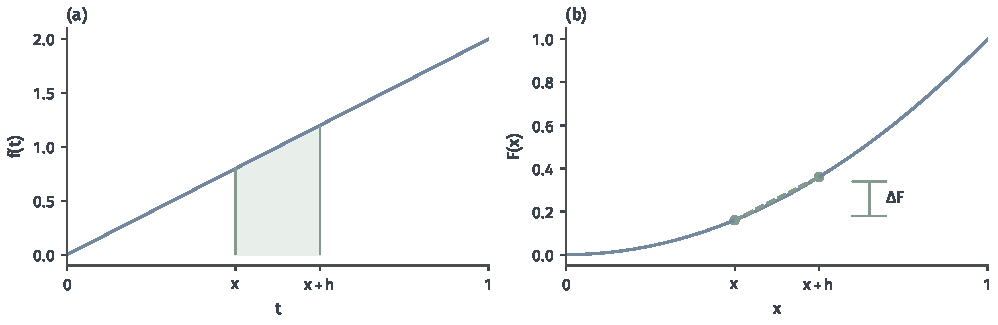
\includegraphics[width=169.0mm]{figures/01-mathematical-preliminaries-upper/01-mathematical-language-combinatorics-analysis-optimization/matplotlib/chapter3-concept-processes/accumulation-increment.pdf}
 \caption{(a) $f(t)=2t$在$[x,x+h]$上的绿色面积。(b) $F(x)=x^2$对应的增量$\Delta F$。图取$x=0.4,h=0.2$，两者都等于$0.2$。将增量除以$h$得到短区间平均值；只有再令$h\to0$，它才趋于$f(x)$，不能把有限平均值直接当作基点导数。}
 \label{fig:analysis-process-accumulation-increment}
\end{figure*}

\subsection{积分的运算法则}
\label{sec:analysis-integral-calculus-rules}

从这里起，本章后续的积分一律采用勒贝格积分；“可积”指绝对值积分有限，非负函数的积分则允许为无穷。
前面已经证明积分的基本性质，现在说明如何用它们计算函数加减、范围分拆、换元与分部积分。

\subsubsection{积分的基本运算}

函数相加与积分范围相加是不同的操作，分别由线性和区域可加性保证。
计算时先检查可测性及绝对可积性，再使用相应等式；正负无穷不能通过移项抵消。

\paragraph{和的积分}
在同一测度空间$(X,\mathcal A,\mu)$上，若实值函数$f,g$均可积，则$|f+g|\leq|f|+|g|$保证$f+g$可积。
定理~\ref{thm:analysis-signed-integral-properties}给出
\[
 \int_X(f+g)\,\mathrm d\mu=\int_Xf\,\mathrm d\mu+\int_Xg\,\mathrm d\mu.
\]
反方向也可将同一范围、同一测度下的两个有限积分合并为和的积分。

\paragraph{差的积分}
两个可积函数的差仍可积，因为$|f-g|\leq|f|+|g|$。同一线性定理给出
\[
 \int_X(f-g)\,\mathrm d\mu=\int_Xf\,\mathrm d\mu-\int_Xg\,\mathrm d\mu.
\]
这里两项都是有限实数，不涉及正负无穷的相减。

\paragraph{数乘的积分}
把被积函数乘以固定实数$c$，积分也乘以$c$。若$f$可积，则$cf$可积，且
\[
 \int_Xcf\,\mathrm d\mu=c\int_Xf\,\mathrm d\mu.
\]
这仍是定理~\ref{thm:analysis-signed-integral-properties}的特例；$c=0$时两侧都为零。

\paragraph{积的积分}
乘积需要另行检查可积性，不能直接套用线性。若$f$可积、$g$可测且$|g|\leq M$几乎处处，其中$M$为有限常数，则$|fg|\leq M|f|$保证$fg$可积。
但即使$f,g,fg$都可积，也不能把乘积的积分拆成两个积分相乘：例如在$[0,1]$上取$f(x)=g(x)=x$，则$\int_0^1fg=1/3$，而$(\int_0^1f)(\int_0^1g)=1/4$。

\paragraph{不交范围的积分}
同一函数在不同范围上的累计，可以用区域可加性分拆。
若$A,B\in\mathcal A$、$A\cap B=\varnothing$，且$f$在$A\cup B$上可积，则定理~\ref{thm:analysis-integral-set-additivity}给出
\[
 \int_{A\cup B}f\,\mathrm d\mu=\int_Af\,\mathrm d\mu+\int_Bf\,\mathrm d\mu.
\]
这与“和的积分”不同：这里改变积分范围，被积函数没有相加。

\paragraph{重叠范围的积分}
若两个范围重叠，分别累计会把交集计算两次，需要减去一次。
对可测$A,B$及在$A\cup B$上可积的$f$，有
\[
 \int_{A\cup B}f\,\mathrm d\mu
 =\int_Af\,\mathrm d\mu+\int_Bf\,\mathrm d\mu-\int_{A\cap B}f\,\mathrm d\mu.
\]
将$A\cup B$拆成$A\setminus B$、$A\cap B$、$B\setminus A$三个不交部分，再用区域可加性即可得到此式。

\paragraph{差集上的积分}
从可测范围$A$中去掉可测子集$B\subseteq A$时，去掉的累计量正是$B$上的积分。
若$f$在$A$上可积，由$A=(A\setminus B)\cup B$的不交分拆，得到
\[
 \int_{A\setminus B}f\,\mathrm d\mu=\int_Af\,\mathrm d\mu-\int_Bf\,\mathrm d\mu.
\]

\paragraph{区间的分拆与方向}
在实轴的勒贝格测度下，有限个端点不影响积分，因而可以在一个中间点拆分区间。
若$f$在$[a,b]$上可积、$a\leq c\leq b$，则
\[
 \int_a^bf(x)\,\mathrm dx=\int_a^cf(x)\,\mathrm dx+\int_c^bf(x)\,\mathrm dx.
\]
区间记号另采用有向约定$\int_b^af=-\int_a^bf$，并令$\int_a^af=0$；普通可测集合上的积分没有这一方向约定。

\paragraph{积分的比较}
被积函数几乎处处的大小关系可以传给积分。若$f,g$可积且$f\leq g$几乎处处，则
\[
 \int_Xf\,\mathrm d\mu\leq\int_Xg\,\mathrm d\mu.
\]
因为$g-f$非负且可积，其积分非负，再由差的积分公式移项即可。

\paragraph{积分的绝对值界}
累计中的正负抵消不会超过绝对值的累计。由$-|f|\leq f\leq|f|$及积分比较得到
\[
 \left|\int_Xf\,\mathrm d\mu\right|\leq\int_X|f|\,\mathrm d\mu.
\]
此处$f$可积，所以不等式两侧均有限。

\paragraph{积分的误差估计}
将绝对值界用于两个可积函数之差，就能控制积分结果的误差：
\[
 \left|\int_Xf\,\mathrm d\mu-\int_Xg\,\mathrm d\mu\right|
 \leq\int_X|f-g|\,\mathrm d\mu.
\]
若进一步有$\mu(X)<\infty$且$|f-g|\leq\eta$几乎处处，则右侧不超过$\eta\mu(X)$。
后面的极限与积分问题将用这一估计，把函数的共同误差转成积分误差。

\subsubsection{换元积分法}
\label{sec:analysis-coordinate-change-integral-applications}

变量替换既改变函数表达，也改变输入集合的测度，导数的绝对值负责一维长度的缩放。
下面使用一一对应的换元，先给可测函数的结论，再说明有向端点的写法。

\paragraph{可测函数的换元公式}
对非负函数，换元要保留全部累计；对有符号函数，还需保证正负部分都有限。
下面用微分同胚条件同时控制可逆性、可测性与局部长度变化。
\begin{theorem}[一维勒贝格积分的换元公式]
\label{thm:analysis-lebesgue-change-variables}
设$I,J\subseteq\mathbb R$为开区间，$T:I\to J$是$C^1$微分同胚，即$T$双射且$T,T^{-1}$连续可微。
对非负勒贝格可测$g:J\to[0,\infty]$，有
\[
 \int_Jg(u)\,\mathrm du=\int_Ig(T(x))|T'(x)|\,\mathrm dx,
\]
允许两边为无穷。若$g:J\to\mathbb R$可测，则$g$在$J$上可积当且仅当$g\circ T\,|T'|$在$I$上可积，此时同一等式给出有限积分值。
\end{theorem}
一般换元定理的证明先将局部长度关系推广到可测集合，再经简单函数及单调逼近推广到非负函数；这里引用这一结论\scite{math-folland1999real}。
有符号版本由先对$|g|$换元、确认绝对可积，再分别对正负部分换元得到。

\paragraph{有向区间的换元}
若$[a,b]\subset I$且$g$在$T([a,b])$上可积，$T$在整个区间严格单调，普通长度累计与有向端点可分别写为
\[
 \int_{T([a,b])}g(u)\,\mathrm du
 =\int_a^b g(T(x))|T'(x)|\,\mathrm dx,
 \qquad
 \int_{T(a)}^{T(b)}g(u)\,\mathrm du
 =\int_a^b g(T(x))T'(x)\,\mathrm dx.
\]
第一式按像区间从左到右累计，第二式的方向保留在端点和$T'$中；两式仍是勒贝格积分。
例如$T(x)=2x$把$[0,1]$变为$[0,2]$，故$\int_0^2u^2\,\mathrm du=\int_0^1(2x)^2\,2\,\mathrm dx=8/3$。

\subsubsection{分部积分法}
\label{sec:analysis-integration-remainders}

乘积求导把两个导数项联系起来，绝对连续函数的端点恢复公式允许积分后把其中一项移到另一侧。
下面直接使用绝对连续条件；连续可微函数是其特例。

\paragraph{分部积分公式}
绝对连续保证导数几乎处处存在、可积且记录全部增量，因此能够给乘积求导式积分。
只知道几乎处处可导仍不充分，前面的康托尔函数已说明这一差别。
\begin{theorem}[勒贝格积分的分部积分公式]
\label{thm:analysis-lebesgue-integration-by-parts}
若$u,v:[a,b]\to\mathbb R$绝对连续，则$uv$绝对连续，$uv'$与$u'v$可积，且
\begin{equation}
 \int_a^bu(x)v'(x)\,\mathrm dx
 =[u(x)v(x)]_a^b-\int_a^bu'(x)v(x)\,\mathrm dx.
\label{eq:analysis-integration-by-parts}
\end{equation}
导数在零测例外上的可测有限取值不影响结果。
\end{theorem}
\begin{proof}
$u,v$连续且有界，导数可积，所以$uv'$与$u'v$可积。
对有限个两两不交区间，有
\[
 \begin{aligned}
 \sum_j|u(b_j)v(b_j)-u(a_j)v(a_j)|
 &\leq\|u\|_\infty\sum_j|v(b_j)-v(a_j)|\\
 &\quad+\|v\|_\infty\sum_j|u(b_j)-u(a_j)|.
 \end{aligned}
\]
两因子的绝对连续性使右侧随区间总长度趋零，故$uv$绝对连续。
在两导数都存在的点，$(uv)'=u'v+uv'$；将绝对连续函数的端点恢复定理用于$uv$，再用有限线性移项，便得公式。
\end{proof}
例如取$u(x)=x$、$v(x)=e^x$，得到$\int_0^1xe^x\,\mathrm dx=[xe^x]_0^1-\int_0^1e^x\,\mathrm dx=1$。
在无穷区间上使用时，先对有限截断应用公式，再分别核查边界项的极限以及两个被积项的绝对可积性，不能无故删除端点项。

\paragraph{Taylor公式的积分余项}
分部积分还能给出Taylor展开的积分余项。设$f$在连接$x_0$和$x_0+h$的线段邻域内
$r+1$阶连续可微，其中$r$为非负整数，令$\phi(t)=f(x_0+th)$。
记
\[
 I_r=\frac1{r!}\int_0^1(1-t)^r\phi^{(r+1)}(t)\,\mathrm dt.
\]
基本定理给出$I_0=\phi(1)-\phi(0)$；对$r\geq1$分部积分，
\[
 I_r=-\frac{\phi^{(r)}(0)}{r!}
       +\frac1{(r-1)!}\int_0^1(1-t)^{r-1}\phi^{(r)}(t)\,\mathrm dt
     =-\frac{\phi^{(r)}(0)}{r!}+I_{r-1}.
\]
逐次代入并用$\phi^{(k)}(0)=h^k f^{(k)}(x_0)$，便得
\begin{equation}
 f(x_0+h)=\sum_{k=0}^r\frac{f^{(k)}(x_0)}{k!}h^k
 +\frac{h^{r+1}}{r!}
   \int_0^1(1-t)^r f^{(r+1)}(x_0+th)\,\mathrm dt.
\label{eq:analysis-taylor-integral-remainder}
\end{equation}
参数化$x_0+th$同时处理正、负$h$。若$|f^{(r+1)}|\leq M$，积分权重的总量为
$1/(r+1)$，故余项不超过$M|h|^{r+1}/(r+1)!$，与前面的中间点余项界一致。
例如立方函数在$r=2$时有$f'''=6$，余项就是
$(h^3/2)\int_0^1 6(1-t)^2\,\mathrm dt=h^3$。
这里的余项为勒贝格积分，连续的高阶导数保证被积函数在有限区间上可积。




\subsection{函数列的极限}
\label{sec:measurable-convergence-and-integrals}
\label{sec:analysis-limit-integral-interchange}
\label{sec:analysis-function-convergence-essential-bounds}

设一列函数趋于$f$，知道每个位置的函数值趋近，还不能直接判断极限是否连续、可微或具有预期的积分。
这三个问题控制的对象不同：连续性比较邻近输入，微分比较差商，积分比较全部范围的累计。
下面先明确收敛方式，再分别回答极限与连续、极限与微分、极限与积分的关系；本节涉及的积分全部为勒贝格积分。

\subsubsection{函数列的收敛方式、判别与关系}
\label{sec:analysis-convergence-mode-relations}

逐点收敛允许每个输入单独选择稳定时刻，一致收敛要求同一个下标控制全部输入，几乎处处收敛则允许固定零测范围上的例外。
先区分这些条件，后面才能说明哪种控制足以保持哪种性质。

\paragraph{点态收敛}

固定一个输入以后，比较的只是一列实数。这里不需要函数可微或可积，甚至不需要
在输入集合上指定距离；函数值仍按实数绝对值比较。
\begin{definition}[点态收敛]
\label{def:analysis-pointwise-almost-everywhere-convergence}
设$X\subseteq\mathbb R$，$f_n,f:X\to\mathbb{R}$。若
\[
 \begin{gathered}
  \forall x\in X,\quad
  \forall\varepsilon>0,\quad
  \exists N=N(x,\varepsilon)\in\mathbb N,\\
  \forall n\geq N,\quad
  |f_n(x)-f(x)|<\varepsilon,
 \end{gathered}
\]
即对每个$x$都有$\lim_n f_n(x)=f(x)$，称$f_n$点态收敛到$f$。点态收敛也称逐点收敛（pointwise convergence）。
\end{definition}


固定$x$以后，点态收敛就是前面已经定义的数列收敛；不同位置可以需要不同的开始下标。

\paragraph{点态收敛的判据}
若还不知道极限函数，可以对每个固定输入使用实数列的柯西收敛准则。
这时各输入仍可各自选择尾部起点，不要求同一个下标适用于全部输入。
\begin{theorem}[函数列点态收敛的柯西判据]
\label{thm:analysis-pointwise-cauchy-criterion}
设$X$非空，$f_n:X\to\mathbb R$。存在$f:X\to\mathbb R$使$f_n$点态收敛到$f$，当且仅当
\[
 \begin{gathered}
 \forall x\in X,\quad\forall\varepsilon>0,\quad
 \exists N=N(x,\varepsilon)\in\mathbb N,\\
 \forall m,n\geq N,\quad |f_m(x)-f_n(x)|<\varepsilon.
 \end{gathered}
\]
\end{theorem}
\begin{proof}
固定$x$，若$f_n(x)$收敛，则实数列的柯西准则给出该条件。
反之，条件使每个$(f_n(x))_n$都是实数柯西列，故都有有限极限；定义$f(x)=\lim_nf_n(x)$，便得到所需的点态极限函数。
\end{proof}

\paragraph{一致收敛}

即使每个输入处的误差最终都很小，开始稳定的时刻仍可能依赖输入。
若希望一次选定迭代次数后就控制全部输入，需要更强的一致条件。

\begin{definition}[函数列的一致收敛]
\label{def:analysis-uniform-convergence}
设$X\subseteq\mathbb R$非空，$f_n,f:X\to\mathbb R$。若
\[
  \forall\varepsilon>0,\quad
  \exists N=N(\varepsilon)\in\mathbb N,\quad
  \forall x\in X,\quad
  \forall n\geq N,\quad
  |f_n(x)-f(x)|<\varepsilon,
\]
就称$f_n$在$X$上一致收敛到$f$。等价地，
\begin{equation}
  \lVert f_n-f\rVert_{\infty}
  :=
  \sup_{x\in X}|f_n(x)-f(x)|
  \longrightarrow0.
\label{eq:analysis-uniform-convergence}
\end{equation}
这里的上确界检查全部输入，不排除任何位置；对一般函数，它可能等于$+\infty$，一致收敛要求这些误差最终有限并趋于零。
\end{definition}


\paragraph{一致收敛的判据}
若尚不知道候选极限，可以改为检查后面的函数是否彼此一致接近。
实数的完备性将各点极限组合为一个函数，共同误差再保证一致收敛。
\begin{theorem}[实值函数列的一致柯西判据]
\label{thm:analysis-uniform-cauchy-criterion}
设$X$非空、$f_n:X\to\mathbb R$。存在$f$使$f_n$在$X$上一致收敛，当且仅当
\[
 \forall\varepsilon>0,\quad\exists N,\quad
 \forall m,n\geq N,\quad\forall x\in X,\quad
 |f_m(x)-f_n(x)|<\varepsilon.
\]
\end{theorem}
\begin{proof}
若一致收敛，三角不等式把两项之差控制为它们到极限的两个一致误差，便得必要性。
反之，每个固定$x$处的实数列是柯西列，故有$f(x)=\lim_n f_n(x)$。
给定$\varepsilon>0$，先取$N$使$m,n\geq N$时对全部$x$有$|f_m(x)-f_n(x)|<\varepsilon/2$。
固定$n\geq N$并令$m\to\infty$，得到$|f(x)-f_n(x)|\leq\varepsilon/2$对全部$x$成立，所以一致收敛。
\end{proof}
此判据不要求各函数有界；若各$f_n$有界，极限与一个固定后项的共同误差有限，故极限也有界。

\paragraph{几乎处处收敛}

勒贝格积分不受可测零测修改影响，因此可以允许函数列在一个固定零测集上不收敛。
\begin{definition}[几乎处处收敛]
\label{def:analysis-almost-everywhere-convergence}
给定测度空间$(X,\mathcal A,\mu)$和实函数$f_n,f$，若存在$E\in\mathcal A$、
$\mu(E)=0$，使
\[
 \forall x\in X\setminus E,\quad
 \forall\varepsilon>0,\quad
 \exists N=N(x,\varepsilon),\quad
 \forall n\geq N,\quad |f_n(x)-f(x)|<\varepsilon,
\]
就称$f_n$在$\mu$下几乎处处收敛到$f$。
\end{definition}
这里是先选一个零测集，再在它的补集上逐点收敛；每个精度和每一项不能任意丢掉
不同的正测度区域。可数个零测例外可以取并后统一，任意不可数个零测集的并却未必零测。
若要求极限仍可测，这里采用各$f_n,f$均可测的版本；在未完备空间中，
不能从几乎处处关系自动推出任意指定的例外点取值可测。

固定非空测度空间$(X,\mathcal A,\mu)$及可测实值函数$f_n,f$；点态与一致收敛本身只用到集合$X$，几乎处处收敛还依赖所选测度$\mu$。

\paragraph{蕴含关系与量词}

定义~\ref{def:analysis-pointwise-almost-everywhere-convergence}、\ref{def:analysis-uniform-convergence}与\ref{def:analysis-almost-everywhere-convergence}改变的是误差控制覆盖哪些点，以及是否允许共同零测例外。
固定同一个极限函数，才能准确比较下面三种陈述。
\begin{theorem}[三种函数列收敛方式的关系]
\label{thm:analysis-convergence-mode-implications}
对上述测度空间及函数列，有
\[
 f_n\text{一致收敛到}f
 \ \Longrightarrow\ f_n\text{点态收敛到}f
 \ \Longrightarrow\ f_n\text{几乎处处收敛到}f.
\]
两个逆命题一般都不成立；这些正向蕴含不要求$\mu(X)<\infty$。
\end{theorem}
\begin{proof}
一致收敛选出的$N(\varepsilon)$同时控制全部$x$，因而也控制任意一个固定$x$，得到点态收敛。
点态收敛在每一点成立，可以在几乎处处收敛的定义中取空的例外集。
\end{proof}

若论证中对每个$n$另有可测零测例外集$N_n$，可先取可数并$N=\bigcup_nN_n$，保留一个适用于全部$n$的共同范围。
后面讨论函数项级数时，把$f_n$换成部分和函数列，以上关系也同样适用。

\paragraph{点态收敛不保证一致收敛}
在$[0,1]$上取$f_n(x)=x^n$。它点态收敛到
\[
 f(x)=
 \begin{cases}
  0,&0\leq x<1,\\
  1,&x=1.
 \end{cases}
\]
每个固定的$0<x<1$都有$x^n\to0$，端点$1$处的函数值与极限值则始终都为$1$，误差为零。
但对每个$n$，$\sup_{x\in[0,1]}|f_n(x)-f(x)|=\sup_{0\leq x<1}x^n=1$，所以收敛不一致。
从量词看，固定$\varepsilon=1/2$后，无论选多大的$N$，在$n=N$时
总能选$x_N=(3/4)^{1/N}<1$，使误差$x_N^N=3/4>\varepsilon$。
失败的位置可以随$n$移动；不能把“每个位置最终变小”改写成“某一轮以后所有位置都小”。
若把范围缩为$[0,a]$，其中$0\leq a<1$，则上确界误差为$a^n\to0$，同一公式又变成一致收敛。

若改把指定极限取为$g\equiv0$，同一列函数仅在勒贝格测度下几乎处处收敛到$g$，并不在$x=1$处收敛到$g$。
$f$与$g$几乎处处相等，但不是逐点相等的函数；不能在比较收敛方式时省去这一差别。


图~\ref{fig:analysis-process-pointwise-uniform-errors}对照“每个位置最终变小”和“同一次数控制全部位置”的差别。
\begin{figure*}[!htbp]
 \centering
 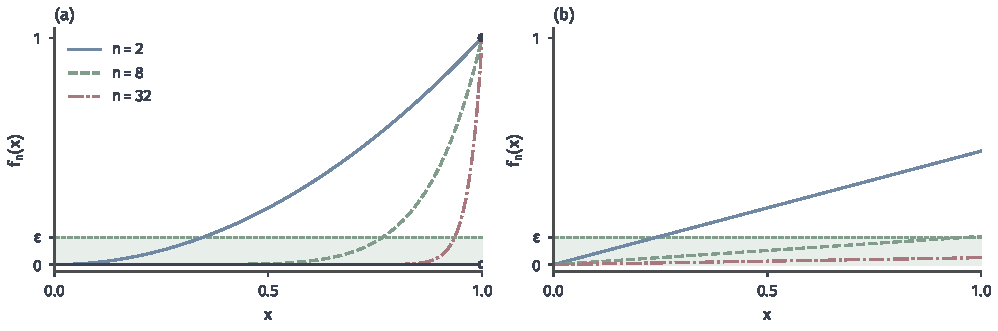
\includegraphics[width=169.0mm]{figures/01-mathematical-preliminaries-upper/01-mathematical-language-combinatorics-analysis-optimization/matplotlib/chapter3-concept-processes/pointwise-uniform-errors.pdf}
 \caption{(a) $f_n=x^n$在$[0,1]$上，黑点与空心点标记逐点极限$\mathbb I_{\{1\}}$；任意有限$n$仍有靠近$1$的输入使误差接近$1$。(b) $g_n=x/n$对所有输入误差均不超过$1/n$。两图绘$n=2,8,32$，绿色带为零附近的$0.12$误差范围；左图在$x=1$处的极限值是$1$，不能将此带误作对该点的误差要求。}
 \label{fig:analysis-process-pointwise-uniform-errors}
\end{figure*}

\paragraph{几乎处处收敛不保证点态收敛}
在$[0,1]$上令$f_n(x)=n\mathbb I_{\{0\}}(x)$，并指定极限为零函数。
在每个$x\neq0$处函数列恒为零，因此几乎处处趋零；在$x=0$处却趋于无穷，连有限的点态极限都不存在。
每个$f_n$都与零函数几乎处处相等，若将原点处的值全部改为零，所得另一列函数便一致收敛到零。
所以零测改值不影响勒贝格积分，却可能改变原来这列函数的点态收敛和一致收敛；这两种收敛检查的是实际取值，不能只由几乎处处等价类决定。

\subsubsection{极限与连续}

逐点收敛只说明固定输入处的变化，不能统一控制邻近输入之间的差，因此不自动保留连续性。
一致收敛提供共同的函数值误差，连续性便可传给极限；局部一致收敛也足够，因为检查某点连续只需它附近的输入。

\paragraph{连续函数的一致极限}
用连续函数逼近一个函数时，需要确认共同误差控制能否把连续性传给极限。
\begin{theorem}[一致极限保持连续性]
\label{thm:analysis-uniform-continuity-limit}
设$X\subseteq\mathbb R$，连续函数$f_n:X\to\mathbb R$一致收敛到$f$，则$f$在$X$上连续。
\end{theorem}
\begin{proof}
固定$a\in X$及$\varepsilon>0$，先选$N$使$\sup_X|f_N-f|<\varepsilon/3$，再由$f_N$在$a$处连续选$\delta$。当$x\in X$且$|x-a|<\delta$时，
\[
 |f(x)-f(a)|
 \leq |f(x)-f_N(x)|+|f_N(x)-f_N(a)|+|f_N(a)-f(a)|<\varepsilon.
\]
所以$f$连续。这里先固定一个对所有输入都适用的$N$，再调用单个$f_N$的连续性。
\end{proof}

前面幂函数列的反例已给出不连续的点态极限，所以逐点收敛不能代替一致收敛。还需区分另一个逆向问题：若将同一函数列限制到$[0,1)$，点态极限为连续函数$0$，但$\sup_{[0,1)}x^n=1$，仍不一致趋零。因此极限连续也不能反推一致收敛。


局部一致收敛指每个点都有一个相对邻域，使函数列在该邻域上一致收敛；将同一定理限制到该邻域，即得极限在该点连续。

同样的三项误差估计也适用于度量空间上的连续函数列，而不只是一元实函数；它保留连续性所用的是共同误差尺度，几乎处处收敛的零测例外不能提供这一尺度。

\subsubsection{极限与微分}

求导要比较缩小输入尺度后的差商，因此函数值一致接近仍可能漏掉快速振荡或尖点。
一种足够的控制是导数一致收敛并固定一个函数值；若只控制导数的积分误差，则可得到绝对连续及几乎处处导数的结论，结论强度不同。

\paragraph{一致收敛与导数}
函数值的一致收敛不能保证导数收敛。例如$f_n(x)=\sin(nx)/n$在$[0,2\pi]$上一致趋于零，因为$\sup|f_n|\leq1/n$；导数$f_n'(x)=\cos(nx)$在$x=0$处始终为$1$，连逐点趋零都不成立。

一致极限还可能不可导。令$f_\varepsilon(x)=\sqrt{x^2+\varepsilon^2}$，则
\[
 0\leq f_\varepsilon(x)-|x|
 =\frac{\varepsilon^2}{\sqrt{x^2+\varepsilon^2}+|x|}\leq\varepsilon.
\]
所以它们在实轴上一致趋于$|x|$，但极限在原点不可导。各近似函数的导数为$x/\sqrt{x^2+\varepsilon^2}$；对$x\neq0$趋于$\operatorname{sign}(x)$，其中正数的符号为$1$、负数的符号为$-1$，在原点导数恒为零。即使规定$\operatorname{sign}(0)=0$，这种导数收敛也不一致：取$x_\varepsilon=\varepsilon^2$，导数值趋零，而$\operatorname{sign}(x_\varepsilon)=1$，误差趋于一。

\paragraph{连续可微函数列导数的一致收敛}
若控制的是导数，还需固定一个函数值，才能排除任意竖直平移。
\begin{theorem}[一致导数逼近与求导保持]
\label{thm:analysis-uniform-derivative-limit}
设$a<b$，$f_n\in C^1([a,b])$。若某个$x_0\in[a,b]$满足$f_n(x_0)\to c$，且$f_n'$在$[a,b]$上一致收敛到$g$，则$f_n$一致收敛到某个$f\in C^1([a,b])$，并有$f(x_0)=c$、$f'=g$。
\end{theorem}
\begin{proof}
对$f_n-f_m$使用中值定理，得到
\[
 |f_n(x)-f_m(x)|\leq |f_n(x_0)-f_m(x_0)|+(b-a)\lVert f_n'-f_m'\rVert_\infty.
\]
右侧随$m,n\to\infty$一致趋零，所以$f_n$一致柯西。实值函数列的一致柯西判据给出一致极限$f$，且$f(x_0)=c$。$f,g$均为连续函数的一致极限，因而连续。

还须证明$f'=g$。给定$\varepsilon>0$，取$N$使$n\geq N$时$\lVert f_n'-g\rVert_\infty<\varepsilon$。对$n,m\geq N$及$x\neq y$，中值定理给出
\[
 |(f_n-f_m)(y)-(f_n-f_m)(x)|\leq2\varepsilon|y-x|.
\]
固定$n\geq N$，令$m\to\infty$，再除以$|y-x|$，可知$f$与$f_n$的差商相差至多$2\varepsilon$。因此
\[
 \begin{aligned}
 \left|\frac{f(y)-f(x)}{y-x}-g(x)\right|
 &\leq2\varepsilon+
 \left|\frac{f_n(y)-f_n(x)}{y-x}-f_n'(x)\right|\\
 &\quad+|f_n'(x)-g(x)|.
 \end{aligned}
\]
先固定这个$n$再令$y\to x$，中间一项趋零，最后一项小于$\varepsilon$。由$\varepsilon$任意，得到$f'(x)=g(x)$；端点使用单侧差商。
\end{proof}
若没有单点收敛条件，$f_n(x)=n$的导数虽全为零，函数值却不收敛；若只有函数值一致收敛，上面的振荡和平滑绝对值例子已经说明求导可能失败。这个证明只用中值定理与一致柯西条件；它不要求先把函数值写成导数的积分。

\paragraph{绝对连续函数列导数按积分误差的收敛}
导数未必一致收敛，但若其绝对误差的总累计趋零，仍能控制所有端点的函数增量。
下面用勒贝格积分给出这一条件，结论不额外承诺极限导数连续。
\begin{theorem}[导数积分误差控制的极限]
\label{thm:analysis-integral-derivative-limit}
设$f_n$在$[a,b]$上绝对连续，$g$勒贝格可积，且某个$x_0\in[a,b]$满足$f_n(x_0)\to c$。
若
\[
 \int_a^b|f_n'(t)-g(t)|\,\mathrm dt\longrightarrow0,
\]
则$f_n$一致收敛到绝对连续函数$f(x)=c+\int_{x_0}^xg(t)\,\mathrm dt$，且$f'=g$几乎处处。
\end{theorem}
\begin{proof}
绝对连续函数的基本定理给出$f_n(x)=f_n(x_0)+\int_{x_0}^xf_n'(t)\,\mathrm dt$，因而
\[
 \sup_{x\in[a,b]}|f_n(x)-f(x)|
 \leq|f_n(x_0)-c|+\int_a^b|f_n'-g|\,\mathrm dt\longrightarrow0.
\]
可积函数的累计绝对连续，且导数几乎处处等于$g$，故得结论。
\end{proof}
导数一致收敛定理给出$C^1$极限；这里的积分误差条件只保证绝对连续和几乎处处求导。

\subsubsection{极限与积分}

积分要控制的是整个范围的累计，逐点误差变小未必排除越来越窄的高峰，也未必排除向更远处扩散的贡献。
先检查极限是否可测，再比较四种条件：有限测度上的一致收敛、非负单调收敛、仅非负时的单向估计，以及共同可积上界下的积分交换。

\paragraph{可测函数的逐点极限}
收敛定理还要对极限函数积分，因此必须先确认极限仍是可测函数。
可数个可测函数的上确界、下确界可测，例如$\{\sup_nf_n>a\}=\bigcup_n\{f_n>a\}$。因此
\[
 \liminf_nf_n=\sup_N\inf_{n\geq N}f_n,\qquad
 \limsup_nf_n=\inf_N\sup_{n\geq N}f_n
\]
都可测；逐点极限存在时也可测。连续函数的逐点极限可能不连续，而可测函数的这一封闭性，使函数逼近更容易留在同一类对象中。

\paragraph{逐点收敛的反例}
每个输入处的误差趋零，未必排除面积集中的窄峰；下面固定峰的形状，比较降低总面积与保持总面积两种变化。
用同一形状比较两列连续函数。在$[0,1]$上记$t_+=\max\{t,0\}$，令
\begin{equation}
 b_n(x)=(1-|2nx-1|)_+,\qquad a_n(x)=2n\,b_n(x),\qquad n\geq1.
\label{eq:measurable-continuous-spikes}
\end{equation}
它们只可能在$[0,1/n]$上非零，顶点位于$1/(2n)$，高度分别为$1$和$2n$。
固定$x>0$后，充分大的$n$使$x>1/n$；在$x=0$处两列始终为零，所以都处处趋零。
由三角形面积计算，它们的勒贝格积分满足
\[
 \int_0^1b_n\,\mathrm dx=\frac1{2n},\qquad \int_0^1a_n\,\mathrm dx=1.
\]
两列均不一致趋零，因为最大高度没有趋零。第一列的积分仍趋零；第二列却有
\begin{equation}
 \int_0^1a_n(x)\,\mathrm dx=1,
 \qquad \int_0^1\lim_{n\to\infty}a_n(x)\,\mathrm dx=0.
\label{eq:analysis-continuous-spike-integral-failure}
\end{equation}
这里各项及极限都可积：一致收敛是保证交换的充分条件，逐点收敛却不足够。
峰顶随$n$移动，逐点极限最终看不到它，积分仍保留整个面积；
下面将检查共同可积上界能否控制这项集中贡献。

\paragraph{有限测度上一致收敛下的积分极限}
\label{sec:analysis-classical-limit-integral}
一致误差乘总测度给出积分误差，因此它在有限测度范围上足以交换极限与积分。
这需要总测度有限，也需要各项确实可积。
\begin{theorem}[有限测度上的一致收敛与积分]
\label{thm:analysis-uniform-lebesgue-integral-limit}
设$(X,\mathcal A,\mu)$为测度空间，$\mu(X)<\infty$，实值可测函数$f_n$可积，并在$X$上一致收敛到$f$。
则$f$可积，且
\begin{equation}
 \int_X|f_n-f|\,\mathrm d\mu
 \leq\mu(X)\|f_n-f\|_\infty\longrightarrow0,
 \qquad \int_Xf_n\,\mathrm d\mu\longrightarrow\int_Xf\,\mathrm d\mu.
\label{eq:analysis-uniform-riemann-limit}
\end{equation}
\end{theorem}
\begin{proof}
逐点极限$f$可测。一致收敛保证可选一个$n_0$使$\|f-f_{n_0}\|_\infty<1$，因此
$\int|f|\leq\int|f_{n_0}|+\mu(X)<\infty$。
对充分大的$n$，把有限的共同误差积分，得到所述绝对误差界；积分差的绝对值不超过这项误差积分。
\end{proof}
在无限测度范围上，一致收敛也不足：$f_n=n^{-1}\mathbb I_{[0,n]}$在实轴上一致趋零，积分却恒为$1$。
因此，下列三项测度论结论改用单调性或共同可积上界控制总累计。

\paragraph{非负可测函数列的单调递增收敛}
记$f_n(x)\uparrow f(x)$表示每个固定$x$处的数列单调增加且趋于$f(x)$；允许忽略零测例外时，例外须包含在同一个可测零测集中。简单函数从下方逼近非负函数时正是这样逐步增加的，下面把阶梯逼近中的积分极限关系推广到任意递增的非负可测函数列\scite{math-folland1999real}。
\begin{theorem}[单调收敛定理]
\label{thm:analysis-monotone-convergence}
设$f_n,f:X\to[0,\infty]$可测，且$f_n(x)\uparrow f(x)$几乎处处，则它们的勒贝格积分满足
\[   \lim_{n\to\infty}\int_X f_n\,\mathrm{d}\mu   =   \int_X f\,\mathrm{d}\mu. \]
两边都允许取$+\infty$。
\end{theorem}
\begin{proof}
把单调性或收敛关系失效的可测零测集并为$N$，并将$f_n$与$f$在$N$上都改为$0$。
修改后的函数仍可测且积分不变，所以可假定$f_n\uparrow f$逐点成立。由
$0\leq f_n\leq f$，积分序列单调不减且
\[   L:=\lim_{n\to\infty}\int f_n\,\mathrm{d}\mu   \leq\int f\,\mathrm{d}\mu. \]
还需证明反向不等式。任取满足$0\leq s\leq f$的简单函数，将它写为 $s=\sum_{j=1}^m a_j\mathbb{I}_{E_j}$，其中$a_j>0$且$E_j$两两不交。固定 $c\in(0,1)$，定义
\[   E_{j,n}   =   E_j\cap\{x:f_n(x)\geq ca_j\}. \]
由于$f_n\uparrow f$且$f\geq a_j$于$E_j$，有$E_{j,n}\uparrow E_j$。
第~\ref{sec:analysis-set-measure-continuity}节已由可数可加性证明测度对递增集合连续，
故$\mu(E_{j,n})\uparrow\mu(E_j)$。同时
\[   f_n   \geq   c\sum_{j=1}^m a_j\mathbb{I}_{E_{j,n}}, \]
从而
\[   L   \geq   \lim_{n\to\infty}   c\sum_{j=1}^m a_j\mu(E_{j,n})   =   c\int s\,\mathrm{d}\mu. \]
先令$c\uparrow1$，再对所有$0\leq s\leq f$的简单函数取上确界。根据非负积分的定义~\eqref{eq:analysis-nonnegative-lebesgue-integral}， $L\geq\int f\,\mathrm{d}\mu$。与前一不等式合并即得结论。
\end{proof}

非负性避免正负无穷相消，单调性保证已经积累的质量不会在后续消失。定理不要求存在可积的统一上界，也不要求各$\int f_n$有限。


在$[0,1]$上枚举有理数为$q_1,q_2,\ldots$，令$E_n=\{q_1,\ldots,q_n\}$。
$\mathbb I_{E_n}$递增到$\mathbb I_{\mathbb Q\cap[0,1]}$，各项及极限的勒贝格积分都为零，单调收敛保证这一逼近不离开可测积分框架。
但非负递增不保证有限积分：在$(0,\infty)$上，$\mathbb I_{(0,n)}\uparrow1$，积分从$n$增加到无穷，仍符合单调收敛等式。

\paragraph{非负可测函数列的下极限与积分估计}

若删除单调要求，只保留非负性，连续尖峰$a_n$说明积分等式可能失败，但仍有一个方向的界。对可能不收敛的函数列，可以用每个位置的下极限比较尾部贡献。

\begin{lemma}[Fatou引理]
\label{lem:analysis-fatou}
若$f_n:X\to[0,\infty]$可测，则关于$\mu$的勒贝格积分满足
\begin{equation}
  \int_X\liminf_{n\to\infty}f_n\,\mathrm{d}\mu
  \leq
  \liminf_{n\to\infty}\int_Xf_n\,\mathrm{d}\mu.
\label{eq:analysis-fatou}
\end{equation}
\end{lemma}
\begin{proof}
令$g_n=\inf_{k\geq n}f_k$。则$g_n$可测， $0\leq g_n\uparrow\liminf_k f_k$。由单调收敛定理，
\[   \int\liminf_k f_k\,\mathrm{d}\mu   =   \lim_{n\to\infty}\int g_n\,\mathrm{d}\mu. \]
对每个$k\geq n$都有$g_n\leq f_k$，故
\[   \int g_n\,\mathrm{d}\mu   \leq   \inf_{k\geq n}\int f_k\,\mathrm{d}\mu. \]
令$n\to\infty$便得到式~\eqref{eq:analysis-fatou}。
\end{proof}

非负条件也不能直接删除。令$g_n=n\mathbb I_{(0,1/n)}$，它是集中在短区间上的矩形尖峰，处处趋零且积分恒为$1$。若改取$u_n=-g_n$，则
$\liminf_n u_n=0$处处成立，而$\int u_n=-1$；原不等式会变成错误的$0\leq-1$。
若另有共同的可积下界$h$使$u_n\geq h$，则可以对$u_n-h\geq0$应用Fatou，
再移去有限的$\int h$。可积下界是可用的推广条件，不是无条件允许负值。

Fatou通常只给一个方向。对式~\eqref{eq:measurable-continuous-spikes}中的$a_n$，左边为零、右边为一，不等式严格成立。积分贡献集中在越来越小的区间内，逐点极限没有保留它。下面图~\ref{fig:analysis-convergence-obstacles}左侧的矩形尖峰提供同样的机制：它与连续三角尖峰的连续性不同，积分失效的原因相同。右侧回顾前面的求导反例，说明积分与导数需要各自的误差控制。

\paragraph{共同可积上界下的收敛与积分}

若函数会振荡或有正负值，单调条件未必可用，可以改用同一个非负可积函数$g$控制所有$|f_n|$，让局部高峰和远处尾部都受有限总量限制。每个$f_n$分别可积还不够，下面要求的是一项覆盖整列函数的共同控制。

\begin{theorem}[支配收敛定理]
\label{thm:analysis-dominated-convergence}
设$f_n,f:X\to\mathbb{R}$可测，$f_n\to f$几乎处处，并且存在非负勒贝格可积函数$g$使
$|f_n|\leq g$几乎处处对所有$n$成立，则$f$勒贝格可积，而且勒贝格积分满足
\[   \lim_{n\to\infty}\int_Xf_n\,\mathrm{d}\mu   =   \int_Xf\,\mathrm{d}\mu. \]
此外，$\int|f_n-f|\,\mathrm{d}\mu\to0$。
\end{theorem}
\begin{proof}
把收敛或控制条件失效的可测零测集的可数并记为$N$，并将$f_n,f,g$在$N$上都改为
$0$。这些函数仍可测且积分不变，因而下述关系可以按逐点意义使用。
由$|f_n|\leq g$并取逐点极限可得$|f|\leq g$几乎处处，所以$f$可积。函数$g+f_n$与$g-f_n$均非负。对它们分别使用Fatou引理，
\begin{align*}
  \int g+\int f
  &\leq
  \int g+\liminf_{n\to\infty}\int f_n,\\
  \int g-\int f
  &\leq
  \int g-\limsup_{n\to\infty}\int f_n.
\end{align*}
由于$\int g<\infty$，可以从两边减去它，得到
\[   \int f   \leq\liminf_n\int f_n   \leq\limsup_n\int f_n   \leq\int f. \]
故积分收敛到$\int f$。

最后，$|f_n-f|\to0$几乎处处，且 $|f_n-f|\leq2g$。再对非负函数$|f_n-f|$应用刚证明的积分交换结论，得到 $\int|f_n-f|\,\mathrm{d}\mu\to0$。
\end{proof}


在$[0,1]$上，幂函数列$x^n$几乎处处趋零，且被可积常数一支配，故积分趋零；这与它不一致收敛没有矛盾。连续尖峰$b_n$也满足$0\leq b_n\leq1$，所以支配收敛给出$\int b_n\to0$。面积保持为一的$a_n$则没有共同可积支配，下面直接检查这一缺口。

假设存在非负可积的$g$使$g\geq a_n$几乎处处对每个$n$成立。
则$1=\int_0^1a_n\leq\int_{[0,1/n]}g$。
但$[0,1/n]$的测度趋零，前面证明的绝对积分的小集合估计使右侧趋零，矛盾。
所以这里并非支配函数暂时没有找到，而是这种可积支配根本不存在。

贡献也可以向无穷远移动：在$\mathbb R$上令$f_n=\mathbb I_{[n,n+1)}$，则处处趋零且积分恒为一。它虽共用常数上界一，那个上界在整条实轴上不可积。支配函数本身可以无界；后面的反常积分部分计算端点附近的累计后，再给出这样的例子。

\begin{figure*}[htbp]
  \centering
  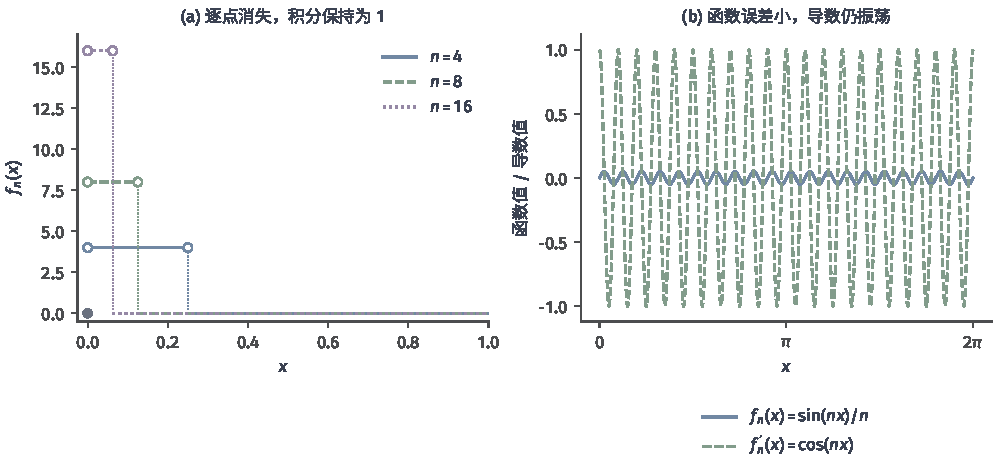
\includegraphics[width=169.0mm]{figures/01-mathematical-preliminaries-upper/01-mathematical-language-combinatorics-analysis-optimization/matplotlib/analysis-convergence-obstacles/figure.pdf}
  \caption{两种交换运算的障碍。左图的尖峰支撑不断收缩，但高度同步增长，每条曲线的积分仍为$1$；开圆点标出不取的上端点，竖虚线仅提示跳跃。右图取$n=20$，$\sin(nx)/n$的函数幅度很小，导数$\cos(nx)$仍有单位幅度。两图均为按给定函数公式构造的教学示例。}
 \label{fig:analysis-convergence-obstacles}
\end{figure*}

表~\ref{tab:analysis-interchange-conditions}汇总极限与勒贝格积分交换的不同条件。积分等式成立的依据来自这些条件，不能仅由已经存在的点态极限推出。
\begin{table*}[htbp]
 \centering\small
 \begin{tabularx}{\linewidth}{@{}lXX@{}}
 \toprule
 结果 & 核对的条件 & 可得到的结论\\
 \midrule
 有限测度上一致收敛 & 各项可积，且全部输入的误差一致趋零 & 极限可积，积分可交换极限\\
 单调收敛 & 非负可测函数逐点或几乎处处递增 & 极限与积分相等，允许无穷值\\
 Fatou引理 & 非负可测函数列 & 先取下极限再积分，不超过先积分再取下极限的结果\\
 支配收敛 & 几乎处处收敛，且共用一个可积绝对上界 & 积分可交换极限，并有$\int|f_n-f|\,\mathrm d\mu\to0$\\
 \bottomrule
 \end{tabularx}
 \caption{极限与勒贝格积分之间的交换条件。表中的测度、可测性和统一控制属于结论的假设。}
 \label{tab:analysis-interchange-conditions}
\end{table*}


这些结论控制的运算不同：保留连续性使用共同函数值误差，交换微分还要控制导数；交换积分则检查有限测度、非负单调性或共同可积支配等相应条件。表~\ref{tab:analysis-interchange-conditions}中的条件及前面的反例给出了各自的适用边界。

\subsection{函数项级数的极限}
\label{sec:analysis-function-series-limits}

函数列的极限比较一列已经给定的函数；函数项级数则把不断加入的函数项累计起来。
给定$u_n:X\to\mathbb R$，记部分和$S_N(x)=\sum_{n=1}^Nu_n(x)$，研究$\sum_{n=1}^\infty u_n(x)$就是研究函数列$(S_N)$。
下面先按部分和区分收敛方式，再判断何时收敛，以及求导或积分能否移入无穷求和。

\subsubsection{收敛方式与判别}

部分和把级数化成函数列，前面几种收敛方式都可以沿用，但必须说明它们约束的是部分和，而不是单个函数项$u_n$。

\paragraph{点态收敛}
若对每个$x\in X$，实数级数$\sum_nu_n(x)$有有限和$u(x)$，就称函数项级数点态收敛到和函数$u$，即$S_N(x)\to u(x)$。
尾部起点可以随$x$改变。特别地，$u_n(x)\to0$只是必要条件，不能代替部分和收敛。

\paragraph{点态收敛的判据}
未知和函数时，比较两个较晚的部分和；它们的差是一段有限尾和，因此点态收敛等价于：
\[
 \begin{gathered}
 \forall x\in X,\quad\forall\varepsilon>0,\quad\exists N=N(x,\varepsilon),\\
 m>n\geq N\Longrightarrow
 \left|\sum_{k=n+1}^{m}u_k(x)\right|<\varepsilon.
 \end{gathered}
\]
这是将定理~\ref{thm:analysis-pointwise-cauchy-criterion}用于$S_N$，与数项级数逐点使用柯西准则完全一致。

\paragraph{一致收敛}
若部分和函数列在$X$上一致收敛到$u$，就称函数项级数在$X$上一致收敛，即
\[
 \sup_{x\in X}|S_N(x)-u(x)|\longrightarrow0.
\]
同一个$N$控制全部输入处的剩余和。例如在$[0,1)$上，$\sum_{n=0}^\infty x^n$逐点收敛到$1/(1-x)$，但每个有限部分和有界而和函数无界，不可能一致收敛。
若每个$u_n$连续，有限部分和也连续，一致收敛便由定理~\ref{thm:analysis-uniform-continuity-limit}保证和函数连续。

\paragraph{一致收敛的判据}
若希望得到一致收敛，就要把尾部起点放在选择输入之前。
由定理~\ref{thm:analysis-uniform-cauchy-criterion}，一致收敛当且仅当
\[
 \begin{gathered}
 \forall\varepsilon>0,\quad\exists N,\quad\forall x\in X,\\
 m>n\geq N\Longrightarrow
 \left|\sum_{k=n+1}^{m}u_k(x)\right|<\varepsilon.
 \end{gathered}
\]
这里不预先指定和函数，实数的完备性先提供各点极限，共同尾和界再使收敛一致。

\paragraph{几乎处处收敛}
在测度空间$(X,\mathcal A,\mu)$上，若存在一个可测零测集$E$，使$S_N(x)$在每个$x\notin E$处收敛到$u(x)$，就称级数几乎处处收敛。
各函数项可测时，可以把和函数在$E$上取零以保留可测性。它与点态收敛的区别是允许固定的零测例外，并未提供全域共同的误差界。

\paragraph{绝对收敛}
若对每个$x$都有$\sum_n|u_n(x)|<\infty$，就称函数项级数在各点绝对收敛；只在零测集外成立时称几乎处处绝对收敛。
这能保证相应位置的级数收敛，却不自动给出一致收敛；后者还需要全部输入共同适用的尾和控制。

\paragraph{Weierstrass判别法}
逐一估计所有输入处的尾和可能困难。若每项都能用一个与输入无关的非负数控制，就可把函数项级数归约为已知的数项级数。
\begin{theorem}[Weierstrass判别法]
\label{thm:analysis-weierstrass-series-test}
设$X$非空，$u_n:X\to\mathbb R$。若存在非负实数$M_n$使
\[
 \forall x\in X,\quad |u_n(x)|\leq M_n,
 \qquad \sum_{n=1}^{\infty}M_n<\infty,
\]
则$\sum_nu_n$在每个$x$处绝对收敛，并在$X$上一致收敛到某个实值函数$u$。
此外，截断误差满足
\[
 \sup_{x\in X}\left|u(x)-\sum_{n=1}^Nu_n(x)\right|
 \leq\sum_{n>N}M_n\longrightarrow0.
\]
\end{theorem}
\begin{proof}
对每个固定$x$，比较判别给出$\sum_n|u_n(x)|\leq\sum_nM_n<\infty$，故和$u(x)$存在。
对任意$m>N$，三角不等式给出$|\sum_{n=N+1}^m u_n(x)|\leq\sum_{n>N}M_n$。
令$m\to\infty$并对$x$取上确界，就得到所述误差界；数项级数的尾和趋零，故收敛一致。
\end{proof}
例如在$[-1,1]$上，$u_n(x)=x^n/2^n$满足$|u_n(x)|\leq2^{-n}$，而$\sum_{n>N}2^{-n}=2^{-N}$。
这个共同的几何尾和控制全部输入处的截断误差；每个函数项连续，所以和函数也连续。
判别法是充分条件，不能把“没有找到这样的$M_n$”当成不一致收敛的证明。

\subsubsection{逐项求导}

部分和总可以有限次求导，问题在于求导后再取极限，是否得到和函数的导数。
单靠原级数一致收敛仍不够；下面把控制施加在导数级数，并用一个点的函数值确定累计常数。
\begin{theorem}[函数项级数的逐项求导]
\label{thm:analysis-function-series-differentiation}
设$u_n\in C^1([a,b])$。若存在$x_0\in[a,b]$使$\sum_nu_n(x_0)$收敛，且导数级数$\sum_nu_n'$在$[a,b]$上一致收敛，则$\sum_nu_n$在$[a,b]$上一致收敛到某个$u\in C^1([a,b])$，且
\[
 u'(x)=\sum_{n=1}^{\infty}u_n'(x).
\]
\end{theorem}
\begin{proof}
取$S_N=\sum_{n=1}^Nu_n$，则$S_N(x_0)$收敛，$S_N'=\sum_{n=1}^Nu_n'$一致收敛。
将函数列导数的一致收敛结论（定理~\ref{thm:analysis-uniform-derivative-limit}）用于$S_N$，即得原级数一致收敛、和函数连续可微以及导数公式。
\end{proof}
例如可用Weierstrass判别法检查导数级数的一致收敛；这与直接检查原级数的共同上界是两件事。
若函数项只有绝对连续性，也可将定理~\ref{thm:analysis-integral-derivative-limit}用于部分和：单点级数收敛且导数部分和按绝对误差积分趋于某个可积函数$g$时，和函数绝对连续，并有$u'=g$几乎处处。
这里$g$是导数部分和的积分误差极限，不能额外断言导数级数在每个点都收敛。

\subsubsection{逐项积分}

将有限部分和的积分写成有限和总是允许的，能否再令项数趋于无穷，则取决于部分和的积分控制。
非负项、绝对积分总和有限以及有限测度上的一致收敛，给出三种不同的充分条件。

\paragraph{非负函数项级数的逐项积分}
非负项使部分和递增，因此可以直接使用前面的单调收敛结论，不要求总积分有限。
\begin{theorem}[非负函数项级数的逐项积分]
\label{thm:analysis-nonnegative-series-integration}
若$u_n:X\to[0,\infty]$可测，则
\[
 \int_X\sum_{n=1}^{\infty}u_n\,\mathrm d\mu
 =\sum_{n=1}^{\infty}\int_Xu_n\,\mathrm d\mu,
\]
两边均允许为$+\infty$。
\end{theorem}
\begin{proof}
非负部分和$S_N$递增到$\sum_nu_n$。用单调收敛定理交换极限与积分，再对每个$S_N$用有限加法，即得等式。
\end{proof}

\paragraph{绝对积分总和有限时的逐项积分}
有正负项时，绝对累计可以同时控制无限求和中的抵消及积分误差。
下面的条件既保证和函数可积，也保证部分和按绝对误差积分趋于和函数。
\begin{theorem}[绝对积分可求和的函数项级数]
\label{thm:analysis-absolutely-integrable-series}
若$u_n:X\to\mathbb R$可测且$\sum_n\int_X|u_n|\,\mathrm d\mu<\infty$，则$\sum_nu_n$几乎处处绝对收敛。
将和函数在绝对值级数发散的可测零测集上定义为零，所得$u$可积，并有
\[
 \int_X\left|u-\sum_{n=1}^Nu_n\right|\,\mathrm d\mu
 \leq\sum_{n>N}\int_X|u_n|\,\mathrm d\mu\longrightarrow0,
\]
从而
\[
 \int_Xu\,\mathrm d\mu=\sum_{n=1}^{\infty}\int_Xu_n\,\mathrm d\mu.
\]
\end{theorem}
\begin{proof}
由非负级数的逐项积分，$G=\sum_n|u_n|$满足$\int_XG\,\mathrm d\mu<\infty$，故$G<\infty$几乎处处。
在可测零测集$E=\{G=\infty\}$之外，级数绝对收敛，且$|u|\leq G$；在$E$上取$u=0$后，$u$仍可测且可积。
对几乎每个$x$，$|u(x)-S_N(x)|\leq\sum_{n>N}|u_n(x)|$。
对这一不等式积分，再对右侧非负尾级数逐项积分，得到所述误差界。
积分差不超过绝对误差积分，而有限部分和满足$\int S_N=\sum_{n=1}^N\int u_n$，令$N\to\infty$便得到结论。
\end{proof}

\paragraph{有限测度上一致收敛时的逐项积分}
还有一种充分条件直接约束部分和的共同误差，而不要求绝对积分的总和有限。
若$\mu(X)<\infty$、各$u_n$可积，且部分和$S_N$一致收敛到$u$，则定理~\ref{thm:analysis-uniform-lebesgue-integral-limit}给出
\[
 \int_Xu\,\mathrm d\mu
 =\lim_{N\to\infty}\int_XS_N\,\mathrm d\mu
 =\sum_{n=1}^{\infty}\int_Xu_n\,\mathrm d\mu.
\]
这里的关键是有限总测度乘一致误差趋零；它与上一段的绝对可求和条件应分别检查。

\subsection{反常积分}
\label{sec:analysis-improper-integrals}

前面的有限区间计算还留下两个问题：积分范围延伸到无穷远时怎样累计，函数在端点或内部位置无界时怎样累计。
这两类问题通常称为\term{反常积分}（improper integral）。下面先分别说明定义与截断方式，再集中判断何时可积。
本节沿用勒贝格积分约定：非负函数的积分允许为无穷，有符号函数的有限可积性要求绝对值积分有限；截断用来计算已有的积分，不把指定顺序下的抵消另算作有限勒贝格积分。

\subsubsection{无穷区间上反常积分的定义}

先设$f$在每个有限区间$[a,R]$上勒贝格可积，唯一待处理的部分是无穷远处的尾部。
把积分范围延伸到半轴，就得到这一类反常积分的记号。
\begin{definition}[无穷区间上的反常积分]
\label{def:analysis-improper-infinite-interval}
设$f:[a,\infty)\to\mathbb R$可测，且在每个$[a,R]$上可积。
将$[a,\infty)$上的勒贝格积分记为
\[
 \int_a^\infty f(x)\,\mathrm dx:=\int_{[a,\infty)}f\,\mathrm dm,
\]
称为无穷区间上的反常积分。
若$f\geq0$，该值属于$[0,\infty]$；若$f$有正负值，本节讨论其有限积分时要求$\int_a^\infty|f|<\infty$。
\end{definition}
这个记号可以通过有限范围上的计算求值。非负时由单调收敛，有
\[
 \int_a^\infty f(x)\,\mathrm dx
 =\lim_{R\to\infty}\int_a^R f(x)\,\mathrm dx,
\]
允许为无穷；有符号且绝对可积时，对$f\mathbb I_{[a,R]}$使用$|f|$支配，也得到同一有限等式。
严格说，可先沿$R_n\uparrow\infty$应用函数列的收敛结论；非负累计的单调性或遗漏范围的绝对积分趋零，再保证任意$R\to\infty$时结论相同。

左半轴作相同处理。整个实轴上还需分别处理左右两端：对任意固定$c\in\mathbb R$，$f$可积当且仅当两侧的绝对值积分都有限，此时
\[
 \int_{\mathbb R}f\,\mathrm dm
 =\int_{(-\infty,c]}f\,\mathrm dm+\int_{(c,\infty)}f\,\mathrm dm.
\]
只知道对称截断$[-R,R]$中的正负抵消稳定，不能代替左右两侧可积。

\subsubsection{无界函数反常积分的定义}

范围有限时，函数仍可能在端点附近无界。先避开该端点计算，再检查遗漏的短区间是否保留了不可忽略的累计。
\begin{definition}[无界函数的反常积分]
\label{def:analysis-improper-unbounded-function}
设$f:(a,b]\to\mathbb R$可测，在每个$[c,b]$（$a<c<b$）上可积，并允许在$a$附近无界。
将$(a,b]$上的勒贝格积分记为
\[
 \int_a^bf(x)\,\mathrm dx:=\int_{(a,b]}f\,\mathrm dm,
\]
称为在端点$a$处的反常积分。
若$f\geq0$，该值允许为$+\infty$；若$f$有正负值，本节讨论其有限积分时要求$\int_{(a,b]}|f|\,\mathrm dm<\infty$。
\end{definition}
非负时，$f\mathbb I_{[c,b]}$随$c\downarrow a$逐步增加到$f$；有符号且绝对可积时，这些截断函数由$|f|$支配。
因此分别用单调收敛或支配收敛得到
\[
 \int_{(a,b]}f\,\mathrm dm=\lim_{c\downarrow a}\int_c^bf(x)\,\mathrm dx.
\]
若无界位置在右端点，就从左侧截断；若在内部点$s$，则把$(a,s)$与$(s,b)$分开累计，有符号有限积分要求两侧均绝对可积。
在单点上赋予可测有限值不改变勒贝格积分，因而判断可积性的是附近的累计，并非该点取了什么值。


图~\ref{fig:analysis-process-improper-two-truncations}对照两种截断：向外扩大累计范围，或从奇点附近逐渐补回遗漏范围。
\begin{figure*}[!htbp]
 \centering
 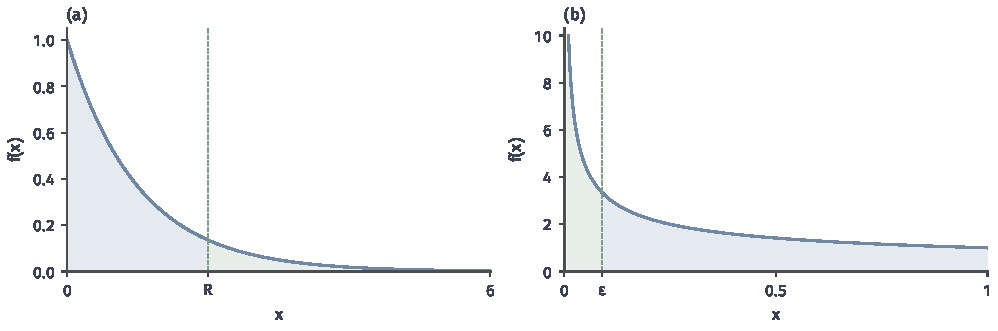
\includegraphics[width=169.0mm]{figures/01-mathematical-preliminaries-upper/01-mathematical-language-combinatorics-analysis-optimization/matplotlib/chapter3-concept-processes/improper-two-truncations.pdf}
 \caption{(a) $e^{-x}$在$[0,\infty)$上，以$R=2$截断，蓝区已计入，绿区属于遗漏尾部，其完整积分为$e^{-2}$；图只显示到$x=6$。(b) $x^{-1/2}$在$(0,1]$上，以$\varepsilon=0.09$截断，完整遗漏积分为$2\sqrt\varepsilon$。右图曲线只绘$x\geq0.01$，未画出的更近零点部分仍属积分范围。}
 \label{fig:analysis-process-improper-two-truncations}
\end{figure*}

\subsubsection{反常积分的可积性}

两种截断都可以写为递增可测范围$E_n\uparrow X$：范围不断延伸，或者从被避开的奇异位置逐步收回遗漏部分。
因此可以用同一个判据回答可积性问题，随后再用截断积分或原函数计算具体数值。

\paragraph{简单函数与截断函数的积分收敛}
对非负可测$f$，前面的规范简单函数$s_n$逐点递增到$f$，单调收敛定理现在补上$\int s_n\uparrow\int f$。若$f$绝对可积，截断$f_n=\max\{-n,\min\{f,n\}\}$满足$f_n\to f$且$|f_n|\leq|f|$，支配收敛给出$\int|f_n-f|\to0$。在实轴上再令截断范围$[-n,n]$扩大，所得$f\mathbb I_{[-n,n]}$也被$|f|$支配；这与前面的无穷范围截断相对应，说明有限范围上的计算可以逼近全域积分。

\paragraph{非负函数的可积性}
非负累计随截断范围扩大而增加，存在有限积分的关键是这些累计能否被同一个有限常数控制。
\begin{theorem}[非负截断累计的有界判据]
\label{thm:analysis-improper-nonnegative-criterion}
设$f:X\to[0,\infty]$可测，$E_n$为递增可测集且$\bigcup_nE_n=X$。则
\[
 \int_Xf\,\mathrm d\mu<\infty
 \quad\Longleftrightarrow\quad
 \sup_n\int_{E_n}f\,\mathrm d\mu<\infty,
\]
并有$\int_Xf\,\mathrm d\mu=\lim_n\int_{E_n}f\,\mathrm d\mu$。
\end{theorem}
\begin{proof}
因为$0\leq f\mathbb I_{E_n}\uparrow f$，单调收敛定理使全域积分等于截断积分序列的极限，也就是其上确界。
因此全域积分有限恰好等价于这些截断积分有共同有限上界。
\end{proof}
在无穷半轴上可取$E_n=[a,a+n]$，在奇异端点$a$附近可取$E_n=[a+(b-a)/(n+1),b]$。
只知道每一个截断积分分别有限不够，还要检验它们是否共同有界。

若$0\leq f\leq g$几乎处处且$\int g<\infty$，则$\int f<\infty$。
反之，若$0\leq g\leq f$且$\int g=\infty$，则$\int f=\infty$。
例如在$(0,1)$上，用单调截断与幂函数原函数计算，得到
\[
 \int_0^1x^{-1/2}\,\mathrm dx=\lim_{n\to\infty}2(1-n^{-1/2})=2,
 \qquad
 \int_0^1x^{-1}\,\mathrm dx=\lim_{n\to\infty}\log n=+\infty.
\]
在$[1,\infty)$上，$\int_1^\infty x^{-2}\,\mathrm dx=1$，而$\int_1^\infty x^{-1}\,\mathrm dx=+\infty$。
这几项计算始终使用同一勒贝格积分定义，极限等式由单调收敛保证。

以正函数$x^{-p}$说明位置的重要性。对$p>0$，在$[2^k,2^{k+1}]$上的累计满足
\[
 2^{-p}2^{k(1-p)}\leq\int_{2^k}^{2^{k+1}}x^{-p}\,\mathrm dx\leq2^{k(1-p)}.
\]
这是把函数在该段的最小值和最大值分别乘区间长度。$p>1$时上界随$k$几何衰减，有限几何和有共同上界，所以尾部积分收敛；$0<p\leq1$时各段至少贡献一个不趋零的正量，累计发散。$p\leq0$时$x^{-p}\geq1$于$x\geq1$，也发散。

同样比较靠近$0$的各段$[2^{-(k+1)},2^{-k}]$，在$p>0$时累计介于$2^{k(p-1)}/2$与$2^{p-1}2^{k(p-1)}$之间，故局部累计恰在$p<1$时有限；$p\leq0$时函数还能连续延拓到$0$，本来就可积。于是$\int_0^1x^{-p}\,\mathrm dx$恰在$p<1$时有限，$\int_1^\infty x^{-p}\,\mathrm dx$恰在$p>1$时有限。分段常数比较与几何级数给出可积性的阈值，原函数则能进一步计算有限截断的具体数值。

\paragraph{有符号函数的可积性}
正负值抵消可能使截断积分保持有限，但可积性要求正、负两部分各自具有有限累计。
因此应把上一段的非负判据用于$|f|$，而不是用于有正负抵消的$f$。
\begin{theorem}[绝对截断累计的可积性判据]
\label{thm:analysis-improper-signed-criterion}
设$f:X\to\mathbb R$可测，$E_n\uparrow X$为可测范围，则$f$可积当且仅当
\[
 \sup_n\int_{E_n}|f|\,\mathrm d\mu<\infty.
\]
可积时，每个截断积分有限，且
\[
 \left|\int_Xf\,\mathrm d\mu-\int_{E_n}f\,\mathrm d\mu\right|
 \leq\int_{X\setminus E_n}|f|\,\mathrm d\mu\longrightarrow0.
\]
所以任意这样的递增穷尽都得到同一个积分值。
\end{theorem}
\begin{proof}
将非负截断判据用于$|f|$，即得充要条件。可积时，区域可加性把积分差写成遗漏范围上的积分，再用绝对值界得到误差不等式。
函数$|f|\mathbb I_{X\setminus E_n}$逐点趋零且由可积的$|f|$支配，故其积分趋零。
\end{proof}
绝对值尾部既用于判断可积性，也控制有限计算的误差。

例如$p>1$时，按$[2^jR,2^{j+1}R]$分段比较得到
\[
 \int_R^\infty x^{-p}\,\mathrm dx
 \leq R^{1-p}\sum_{j=0}^\infty2^{j(1-p)}
 =\frac{R^{1-p}}{1-2^{1-p}}\longrightarrow0.
\]
非负积分的区域可数可加性保证分段求和合法，几何尾和给出显式误差界。

有了$x^{-1/2}$的可积性，就能核对无界支配的例子：在$(0,1)$上，$x^n/\sqrt x\to0$处处，
且$0\leq x^n/\sqrt x\leq x^{-1/2}$，因此支配收敛保证积分趋零。
截断后由原函数计算也得$\int_0^1x^{n-1/2}\,\mathrm dx=(n+1/2)^{-1}\to0$。
支配条件要求共同上界的绝对累计有限，不要求上界本身有界。

积分有限要求正负两部分都有限，不能从某一列截断积分有有限极限直接推出。
下面的例子只说明这种推断为什么失效，不把截断相消作为新的积分规则。

连续函数也可能出现截断相消。在$[1,\infty)$上，分部积分给出
\[
 \int_1^R\frac{\sin x}{x}\,\mathrm dx
 =\cos1-\frac{\cos R}{R}-\int_1^R\frac{\cos x}{x^2}\,\mathrm dx.
\]
端点项有极限，最后一项由$x^{-2}$控制而绝对收敛，所以截断积分存在有限极限。
但在每个$[k\pi+\pi/6,k\pi+5\pi/6]$（$k\geq1$）上，$|\sin x|\geq1/2$，
故该段的绝对积分至少为$1/(3(k+1))$。
调和级数发散使$\int_1^\infty|\sin x|/x\,\mathrm dx=+\infty$；
这个有限截断极限依赖正负抵消，不是本章所用的有限勒贝格积分。

在$(-1,1)$上取$f(x)=1/x$，原点赋值为零。
正负部分的积分都为无穷，所以$f$没有有符号勒贝格积分值；但对称截断满足
\[
 \lim_{\varepsilon\downarrow0}\left(
 \int_{-1}^{-\varepsilon}\frac{\mathrm dx}{x}
 +\int_{\varepsilon}^{1}\frac{\mathrm dx}{x}\right)=0.
\]
这个对称相消极限称为柯西主值。它没有使$\int|f|$变有限，也没有定义出本章采用的勒贝格积分。
后续计算仍只使用非负广义积分或绝对可积函数的有限积分。

\FloatBarrier


\FloatBarrier
\section{本章小结}
\label{sec:analysis-summary}
\label{sec:measurable-summary}

连续性把输入趋近与输出趋近联系起来；一致连续、Lipschitz连续和绝对连续分别加强不同的控制要求。
一元可微性把函数增量写成斜率乘输入增量，中值定理、Taylor余项和导数上界说明局部信息怎样控制有限变化。
测度规定可测集合的大小，同一种距离并不唯一决定集合权重。
有限区间逼近形成Jordan测量，可数覆盖形成外测度，可测分割条件使其在允许的集合族上恢复可数可加等式。
黎曼积分从区间分割出发，勒贝格积分按可测集合及简单函数累计；有界区间上的黎曼可积函数也勒贝格可积，积分值相同，反向包含不成立。
不定积分由原函数定义，变上限积分由累计构造定义，二者的联系需要微积分基本定理。
连续被积函数的累计可逐点求导，勒贝格可积函数一般只保证几乎处处恢复；绝对连续恰好保证函数可以通过可积导数恢复。
连续函数的一致极限连续，微分交换还需控制导数，积分交换还需有限测度、单调性或共同可积支配等条件。
无穷范围与奇点仍按同一积分定义累计，截断方式和绝对值尾部决定计算能否恢复全域积分，指定相消极限不能代替可积性。

\chapter{多元函数微积分}
\label{chap:multivariate-calculus}
\label{chap:multivariable-functions}

当输入由一个实数变为多个坐标时，逐坐标观察是否足以描述整体变化？累计范围由区间变为区域、路径或曲面时，又应使用怎样的权重和方向？
本章使用第~\ref{chap:linear-algebra-and-matrix-analysis}章的向量与线性映射、
第~\ref{chap:function-limits}章的距离与极限，以及第~\ref{chap:univariate-calculus}章的一元微分和勒贝格积分。
先研究联合趋近、全微分与共同的线性近似，再分别建立区域、路径和曲面上的积分。
最后用Green、Gauss和Stokes公式联系内部导数的累计与边界贡献，逐一核对正则性、可积性和定向条件。

\par\Needspace{14\baselineskip}
\section{多元函数的微分}
\label{sec:analysis-multivariable-differentiation}
\label{sec:multivariable-differentiation}

一元微分用一个斜率描述输入微调后的输出变化。对$f(x,y)=x^2+xy+y^2$，输入是二维点而输出仍是一个实数；若同一输入同时产生多个实数，才得到向量值函数。
下面先完整研究多元标量函数，再将线性近似推广到向量输出；矩阵自变量及局部方程的求解各自另作讨论。
这样，梯度始终对应标量输出，Jacobian矩阵始终记录多个输出分量的变化，二者的形状与作用不会混用。
向量、矩阵、迹与行列式沿用第~\ref{chap:sets-functions-and-proofs}章；极限与距离沿用第~\ref{chap:function-limits}章，连续、微分与勒贝格积分沿用第~\ref{chap:univariate-calculus}章的结论。
偏导数与局部线性近似可参考\scite{math-openstax-calculus3}，严格的多元微分论证可参考\scite{math-lebl2026analysis2}。

\subsection{多元标量函数的极限和连续性}
\label{sec:multivariable-limits-continuity}

本小节始终研究$f:D\subseteq\mathbb R^d\to\mathbb R$。多个输入坐标必须共同趋近一个点，输出误差则仍用实数绝对值度量。

\subsubsection{多元标量函数的定义}

固定一个坐标得到一元切片，恢复全部坐标后才是原来的多元函数。先明确输入与输出，才能区分“沿某个切片趋近”和“整个定义域中的趋近”。
\begin{definition}[多元标量函数]
\label{def:multivariable-scalar-function}
设$d$为正整数、$D\subseteq\mathbb R^d$。映射$f:D\to\mathbb R$称为多元标量函数；它把整个输入点$\bm x=(x_1,\ldots,x_d)^\top$映为一个实数$f(\bm x)$。
\end{definition}
例如$f(x,y)=x^2+xy+y^2$在$(1,2)$处取值$7$；固定$y=2$后得到的一元切片是$x\mapsto x^2+2x+4$，它只反映原函数在一条直线上的取值。

\subsubsection{极限的定义与判别}

在实轴上可以从左右两侧趋近，在平面中还可以沿直线、抛物线等路径趋近。
极限必须同时控制所有允许的输入，不能按路径分别选择互不兼容的误差范围。
\paragraph{极限的定义}
\label{sec:multivariable-joint-limits}

设$\bm D\subseteq\mathbb R^d$，$f:\bm D\to\mathbb R$，
$\bm a$是$\bm D$的聚点，即任意小的球内都有不同于$\bm a$的定义域点。
用欧氏距离$\lVert\bm x-\bm a\rVert_2$同时控制各坐标的偏移，便能把一元极限的邻域条件推广过来。
\begin{definition}[多元函数的极限]
\label{def:multivariable-limit}
若对每个$\varepsilon>0$，都存在$\delta>0$，使得
\[
 \bm x\in\bm D,\quad 0<\lVert\bm x-\bm a\rVert_2<\delta
 \quad\Longrightarrow\quad |f(\bm x)-L|<\varepsilon,
\]
则称$f$在$\bm x\to\bm a$时的极限为$L$，记为$\lim_{\bm x\to\bm a}f(\bm x)=L$。
\end{definition}
这里的同一个$\delta$必须控制球内全部允许输入。各坐标可以按不同速度趋近，
也可以让行进方向随位置改变。

\paragraph{序列判据与路径检验}
与一元情形一样，极限存在等价于：任意满足$\bm x_n\in\bm D\setminus\{\bm a\}$、
$\bm x_n\to\bm a$的序列都有$f(\bm x_n)\to L$。
这与一般度量空间中的连续性序列判据结构相同，这里是它在欧氏输入、实数输出下的直接应用，所需的输入与输出距离都已指定。
所以找到两条输出极限不同的路径足以否定极限，但验证有限条路径不能证明极限存在。

\begin{example}[坐标切片与所有直线仍会遗漏路径]
\label{ex:multivariable-path-limits}
令$f(0,0)=0$，非原点处令$f(x,y)=xy/(x^2+y^2)$。
沿两条坐标轴，函数都为$0$；沿$y=x$，函数恒为$1/2$，故原点处没有联合极限。
这个函数分别固定一个坐标后，在另一坐标上连续，但它在原点不联合连续。

即使验证所有过原点的直线，仍不足够。令$g(0,0)=0$，并在非原点处令
\[
 g(x,y)=\frac{x^2y}{x^4+y^2}.
\]
沿$y=kx$，当$k\neq0$时$g(x,kx)=kx/(x^2+k^2)\to0$；
当$k=0$或沿竖直轴时，函数为$0$。
可是沿抛物线$y=x^2$，$g(x,x^2)=1/2$。每条固定直线上的控制不能同时控制弯曲的趋近方式。
\end{example}


图~\ref{fig:analysis-process-joint-limit-paths}把直线路径和弯曲路径放到同一函数上，显示只检查直线可能遗漏的趋近方式。
\begin{figure*}[!htbp]
 \centering
 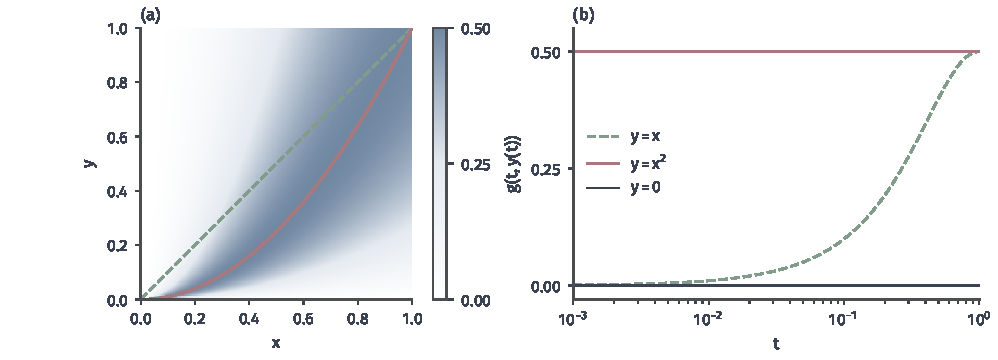
\includegraphics[width=169.0mm]{figures/01-mathematical-preliminaries-upper/01-mathematical-language-combinatorics-analysis-optimization/matplotlib/chapter3-concept-processes/joint-limit-paths.pdf}
 \caption{取前例$g(x,y)=x^2y/(x^4+y^2)$，原点另置零。(a) 第一象限的函数值及三条路径，色阶固定为$0$至$1/2$。(b) 沿$y=0$、$y=x$分别趋零，沿$y=x^2$恒为$1/2$；横轴为正参数$t$的对数刻度，向左趋近原点。不同路径极限足以否定联合极限，有限条路径不能反向证明存在。}
 \label{fig:analysis-process-joint-limit-paths}
\end{figure*}

\paragraph{累次极限与联合极限}
累次极限还会改变问题的量词。先令$y\to0$、再令$x\to0$，考察的是
$\lim_{x\to0}\lim_{y\to0}f(x,y)$，没有要求两个坐标同时趋近。
对上例的$f$，两个次序的累次极限都为$0$，联合极限却不存在。
又如$h(x,y)=x^2/(x^2+y^2)$在非原点定义，则
\[
 \lim_{x\to0}\lim_{y\to0}h(x,y)=1,
 \qquad
 \lim_{y\to0}\lim_{x\to0}h(x,y)=0.
\]
所以累次极限相等不是联合极限存在的充分条件；改变次序也可能改变累次极限。
如果联合极限存在，并且相关内层极限在去心邻域内存在，相应累次极限才必须等于联合极限。

\paragraph{统一误差估计}
要证明联合极限，可以寻找只依赖距离的统一上界。
例如$|xy|\leq(x^2+y^2)/2$，所以
\[
 \left|\frac{x^2y}{x^2+y^2}\right|
 \leq \frac{|x|}{2}
 \leq\frac12\sqrt{x^2+y^2}\longrightarrow0.
\]
这个估计同时覆盖全部路径，因此给出原点极限为$0$。极坐标也可用于估计，
但写成$(x,y)=(r\cos\theta,r\sin\theta)$后，仍需控制所有角度，不能只固定$\theta$再令$r\to0$。

\subsubsection{连续性的定义与运算}
\label{sec:multivariable-continuity}

连续性要求联合趋近时的输出恰好趋于基点值，形式与前面度量下的连续性相同。
这里先对全部输入作共同控制，再讨论运算后能否保留这种控制。
\begin{definition}[多元标量函数的连续性]
\label{def:multivariable-scalar-continuity}
设$f:D\subseteq\mathbb R^d\to\mathbb R$、$\bm a\in D$。若对每个$\varepsilon>0$都存在$\delta>0$，使
\[
 \bm x\in D,\quad\lVert\bm x-\bm a\rVert_2<\delta
 \Longrightarrow |f(\bm x)-f(\bm a)|<\varepsilon,
\]
则称$f$在$\bm a$处连续；在$D$上每点连续时称$f$为连续函数。
\end{definition}
聚点处这等价于联合极限等于$f(\bm a)$，孤立点处则自动成立。固定其他输入坐标后的一元切片连续只是必要条件，例~\ref{ex:multivariable-path-limits}说明它不足以保证联合连续。

\paragraph{和的连续性}
若$f,g$在$\bm a$处连续，则$f+g$也连续，因为和的输出误差不超过两个原误差之和。

\paragraph{差的连续性}
在相同条件下$f-g$连续：差的输出误差同样不超过两个原误差之和。

\paragraph{数乘的连续性}
若$f$在$\bm a$处连续，$c$为固定实数，则$cf$连续。$c\neq0$时将$f$的误差控制在$\varepsilon/|c|$以内即可；$c=0$时结论直接成立。

\paragraph{积的连续性}
若$f,g$在$\bm a$处连续，则$fg$连续。这由两个实数输出的积的极限法则得到。

\paragraph{商的连续性}
若$f,g$在$\bm a$处连续且$g(\bm a)\neq0$，则$g$在基点附近远离零，商的极限法则保证$f/g$连续。分母非零的条件不能省略。
多元多项式由连续坐标函数的有限运算得到，因此连续；分母非零处的有理函数同样连续。

\paragraph{标量复合函数}
若$f:D\to\mathbb R$在$\bm a$处连续，一元函数$\psi$在$f(\bm a)$处连续，且$f$的相邻输出在$\psi$的定义域内，则$\psi\circ f$连续。
先用$\psi$确定中间实数的允许误差，再由$f$控制输入点的欧氏距离，即得到复合函数的误差条件。

\subsubsection{一致连续性与闭有界集上的性质}

一致连续要求同一个输入误差尺度控制全部基点；有界性与最值存在则约束整个定义域上的函数值。
下面用有限维闭有界集内的收敛子列，分别说明这两类整体结论。

\paragraph{有限维闭有界集的收敛子列}
实数列的Bolzano--Weierstrass定理可以逐个坐标使用，得到多维输入所需的子列性质。
这里有界性负责产生收敛子列，闭性则进一步保留极限点。
\begin{theorem}[有限维有界序列的收敛子列]
\label{thm:multivariable-bolzano-weierstrass}
若$(\bm x_n)$是$\mathbb R^d$中的有界序列，则存在严格递增的正整数序列$(n_k)$及$\bm a\in\mathbb R^d$，使$\bm x_{n_k}\to\bm a$。
若所有$\bm x_n$属于闭集$K$，则$\bm a\in K$。
\end{theorem}
\begin{proof}
先用实数列定理选出第一坐标收敛的子列，再从这个子列中选出第二坐标收敛的子列，重复有限次后，全部坐标都收敛。
设各坐标极限组成$\bm a$，由$\lVert\bm x-\bm a\rVert_2\leq\sqrt d\max_j|x_j-a_j|$可知所得子列在欧氏距离下收敛。
若它属于闭集$K$，闭集包含其收敛序列的极限，故$\bm a\in K$。
\end{proof}
有限维闭有界集因此具有前面刚证明的子列性质，下面直接用它证明函数的整体性质；一般度量空间中紧致与序列紧致的等价在第~\ref{chap:metric-spaces}章讨论。

\paragraph{一致连续性}
把连续定义中的$\delta$放在选择基点之前，就得到一致连续的要求。
具体地，对每个$\varepsilon>0$存在$\delta>0$，使所有$\bm x,\bm y\in D$满足$\lVert\bm x-\bm y\rVert_2<\delta$时都有$|f(\bm x)-f(\bm y)|<\varepsilon$。
闭有界集上的逐点连续足以给出这样的共同尺度。
\begin{theorem}[闭有界集上的一致连续性]
\label{thm:multivariable-uniform-continuity}
设$K\subseteq\mathbb R^d$非空、闭且有界，$f:K\to\mathbb R$连续，则$f$在$K$上一致连续。
\end{theorem}
\begin{proof}
定理~\ref{thm:analysis-uniform-continuity}的证明只用到定义域中任意点列都有域内收敛子列，以及连续性。
上一定理已为$K$建立这项子列性质；将输入距离改为欧氏范数，原证明便适用，无需重新构造反例点列。
\end{proof}
存在有限$L$使$|f(\bm x)-f(\bm y)|\leq L\lVert\bm x-\bm y\rVert_2$时，也直接得到一致连续；这是多元标量函数的Lipschitz条件。

\paragraph{有界性与极值达到}
要保证上、下确界由定义域内的点取得，还需要防止取值趋近确界的输入序列逃出定义域。
闭有界集的子列性质正好保留这种极限点。
\begin{theorem}[闭有界集上的极值定理]
\label{thm:multivariable-extreme-value}
设$K\subseteq\mathbb R^d$非空、闭且有界，$f:K\to\mathbb R$连续，则$f$有界，且存在$\bm x_{\min},\bm x_{\max}\in K$满足
\[
 f(\bm x_{\min})\leq f(\bm x)\leq f(\bm x_{\max})\qquad(\bm x\in K).
\]
\end{theorem}
\begin{proof}
定理~\ref{thm:analysis-extreme-value}已证明，定义域内的收敛子列性质与连续性共同保证有界及最值达到。
这里的$K$由定理~\ref{thm:multivariable-bolzano-weierstrass}满足同一子列条件，所以该证明适用，输出仍为实数。
\end{proof}
这些条件是充分保证。整个平面上的$f(x,y)=x^2+y^2$沿$y=0$退化为前面的实轴平方函数反例，所以连续却不一致连续。
在开单位圆盘上，同一函数的上确界为$1$却没有最大点，说明不能直接删去闭性。

\subsection{偏导数和梯度}

下面仍只研究实值函数$f:U\subseteq\mathbb R^d\to\mathbb R$，其中$U$为开集。先计算各坐标切片的变化率，再把这些标量排列为梯度；沿一般方向的变化率也在这里定义。

\subsubsection{偏导数}

开集保证基点附近足够小的双侧坐标扰动仍在定义域内。固定其他坐标后，就可以直接使用一元导数。
\begin{definition}[偏导数]
\label{def:multivariable-partial-derivative}
设$\bm a\in U$，令$\bm e_j$是第$j$个坐标为$1$、其余为$0$的向量。若双侧极限
\[
 \partial_jf(\bm a)=\frac{\partial f}{\partial x_j}(\bm a)
 =\lim_{t\to0}\frac{f(\bm a+t\bm e_j)-f(\bm a)}t
\]
存在且有限，就称它为$f$在$\bm a$处关于$x_j$的\term{偏导数}（partial derivative）。
\end{definition}
它表示只改变第$j$个坐标、其余坐标固定时的变化率。符号$\partial$提醒我们：这里求的是多元函数的一个坐标切片的导数。

例如对$f(x,y)=x^2+xy+y^2$，固定$y$求导得到$f_x=2x+y$；固定$x$得到$f_y=x+2y$。
在$(1,2)$处，两者为$4,5$。具体地，
\[
 \frac{f(1+t,2)-f(1,2)}t=4+t\longrightarrow4.
\]
这里$f_x(1,2)=4$并不意味着同时改变$x,y$时都以斜率$4$变化。每一个偏导数只说明自己的坐标切片。

\subsubsection{梯度}

各偏导数采用相同的基点，但分别对应不同输入坐标。将这些变化率按坐标顺序排列，就能用一个向量记录所有坐标切片的信息。
\begin{definition}[梯度]
\label{def:multivariable-gradient}
若$f:U\to\mathbb R$在$\bm a$处的各一阶偏导数都存在，称列向量
\[
 \nabla f(\bm a)=\bigl(\partial_1f(\bm a),\ldots,\partial_df(\bm a)\bigr)^\top
\]
为$f$在$\bm a$处的\term{梯度}（gradient）。
\end{definition}
对$f(x,y)=x^2+xy+y^2$，有$\nabla f(x,y)=(2x+y,x+2y)^\top$，所以$\nabla f(1,2)=(4,5)^\top$。
梯度的存在只说明各偏导数存在，尚未保证它能预测所有坐标同时改变时的函数增量；这要由后面的可微性判断。

\subsubsection{方向导数}

沿坐标轴求导只是方向变化的一部分。若让多个坐标按一个固定向量共同移动，就得到另一条一元切片。
\begin{definition}[方向导数]
\label{def:multivariable-directional-derivative}
给定向量$\bm v\in\mathbb R^d$，若双侧极限
\[
 D_{\bm v}f(\bm a)
 =\lim_{t\to0}\frac{f(\bm a+t\bm v)-f(\bm a)}t
\]
存在且有限，就称它为沿$\bm v$的\term{方向导数}（directional derivative）。
\end{definition}
本书允许$\bm v$不是单位向量，导数按参数$t$的变化计量；若要表示每单位路程的变化率，应取$\lVert\bm v\rVert_2=1$。
取$\bm v=\bm e_j$便回到偏导数。双侧极限与只令$t\downarrow0$的单侧方向导数要分别判断。

仍取上述$f$，从$(1,2)$沿$\bm v=(1,1)^\top$移动，有
\[
 f(1+t,2+t)=7+9t+3t^2,
 \qquad D_{(1,1)}f(1,2)=9.
\]
改用同向单位向量$\bm u=(1,1)^\top/\sqrt2$，变化率为$9/\sqrt2$。
两者描述同一条直线，但参数速度不同，不能忽略归一化约定。

\subsection{多元标量函数的可微性}
\label{sec:multivariable-total-differentiation}

偏导数和方向导数分别检查固定的坐标轴或直线。若要同时控制任意小扰动，包括方向不断改变的扰动，就需要一个共同的线性近似。

\subsubsection{微分的定义}

预测增量应与扰动的叠加和数乘相容，因此使用线性映射$A:\mathbb R^d\to\mathbb R$。
例如$A(\bm h)=\bm c^\top\bm h$把每个坐标的扰动乘以固定系数再相加；可微性还要求遗漏的误差比扰动长度更小。
\begin{definition}[多元标量函数的可微性与全微分]
\label{def:multivariable-total-differential}
设$U\subseteq\mathbb R^d$开，$f:U\to\mathbb R$，$\bm a\in U$。
若存在一个线性映射$A:\mathbb R^d\to\mathbb R$，使
\begin{equation}
 f(\bm a+\bm h)=f(\bm a)+A(\bm h)+o(\lVert\bm h\rVert_2),
 \qquad\bm h\to\bm0,
\label{eq:analysis-total-differentiability}
\end{equation}
则称$f$在$\bm a$处\term{可微}（differentiable）。线性映射$A$称为该点的\term{全微分}（total differential），记为$\mathrm df_{\bm a}$。
\end{definition}
余项条件是$|f(\bm a+\bm h)-f(\bm a)-A(\bm h)|/\lVert\bm h\rVert_2\to0$。
它要求一个$A$适用于全部趋零扰动，并非先固定一个方向再允许误差控制随方向改变。

\subsubsection{可微性的要求与判别}
\label{sec:analysis-differentiability-relations}

固定开集$U\subseteq\mathbb R^d$、标量函数$f:U\to\mathbb R$与基点$\bm a\in U$。
下面先说明统一线性近似必然满足哪些要求，再给出可核查的充分判别，最后结合蕴含关系与反例，区分偏导数存在、全部双侧方向导数存在、可微和连续可微。

\paragraph{可微的必要条件}
若同一个线性近似有效，它在线性切片上必须与一元导数相同，函数增量本身也必须趋零。
这就把全微分与前面定义的偏导数、梯度及方向导数联系起来。
\begin{theorem}[可微性与梯度、方向导数]
\label{thm:multivariable-differentiable-necessary}
若$f:U\to\mathbb R$在$\bm a$处可微，则$f$在该点连续，各偏导数存在，并且
\[
 \mathrm df_{\bm a}(\bm h)=\nabla f(\bm a)^\top\bm h,
 \qquad D_{\bm v}f(\bm a)=\nabla f(\bm a)^\top\bm v
 \quad(\bm v\in\mathbb R^d).
\]
\end{theorem}
\begin{proof}
线性性给出$A(\bm h)=\sum_jh_jA(\bm e_j)$。由有限和的Cauchy--Schwarz不等式，
\[
 |A(\bm h)|\leq\left(\sum_j|A(\bm e_j)|^2\right)^{1/2}\lVert\bm h\rVert_2.
\]
因此线性项与余项都随$\bm h\to0$而趋零，得到$f$连续。
分别取$\bm h=t\bm e_j$并除以$t$，可知$\partial_jf(\bm a)=A(\bm e_j)$；线性性给出$A(\bm h)=\sum_j\partial_jf(\bm a)h_j$。
再对固定$\bm v$取$\bm h=t\bm v$，余项除以$t$仍趋零，就得到方向导数公式；$\bm v=\bm0$时差商恒为零。
\end{proof}
\begin{example}[二元二次函数的全微分]
\label{ex:multivariable-quadratic-differential}
对二次函数$f(x,y)=x^2+xy+y^2$，在$(1,2)$处有$\nabla f=(4,5)^\top$。设扰动为$(h,k)$，直接展开得
\[
 f(1+h,2+k)=7+4h+5k+(h^2+hk+k^2).
\]
由$|hk|\leq(h^2+k^2)/2$，最后一项绝对值不超过$3(h^2+k^2)/2$。除以$\sqrt{h^2+k^2}$后趋于零，所以全微分确为$4h+5k$。它同时解释了两个偏导数和沿$(1,1)$的变化率$4+5=9$。
\end{example}


图~\ref{fig:analysis-process-total-differential-remainder}将这个全微分的切平面与统一余项界对应起来。
\begin{figure*}[!htbp]
 \centering
 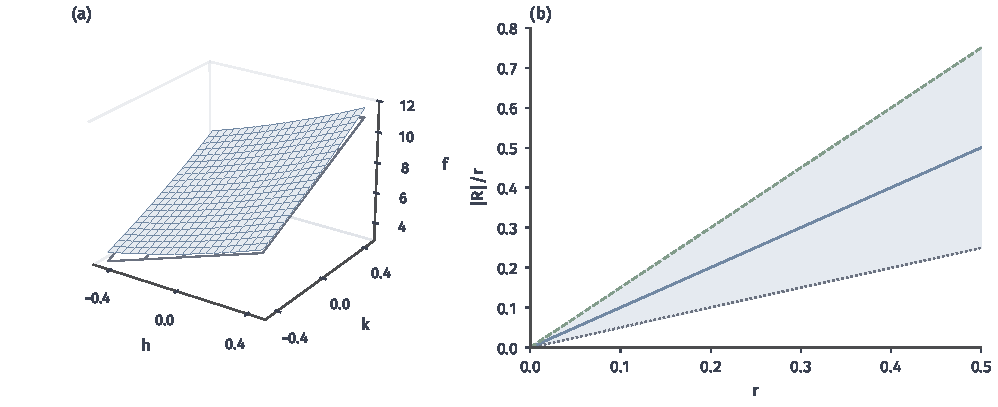
\includegraphics[width=169.0mm]{figures/01-mathematical-preliminaries-upper/01-mathematical-language-combinatorics-analysis-optimization/matplotlib/chapter3-concept-processes/total-differential-remainder.pdf}
 \caption{对二次函数在$(1,2)$处，灰网格是$P=7+4h+5k$，蓝面是$f(1+h,2+k)$。(b) 令$r=\sqrt{h^2+k^2}$，余项$R=h^2+hk+k^2$满足$r/2\leq R/r\leq3r/2$；阴影给出所有方向的完整范围，三条线是其中的代表值。共同上界随$r\to0$趋零，才保证任意方向都适用同一个线性近似。}
 \label{fig:analysis-process-total-differential-remainder}
\end{figure*}

对单位方向$\bm u$，内积不等式给出$D_{\bm u}f(\bm a)\leq\lVert\nabla f(\bm a)\rVert_2$。
当梯度非零时，在$\bm u=\nabla f(\bm a)/\lVert\nabla f(\bm a)\rVert_2$处取等号，故可微函数的梯度方向是局部上升最快的单位方向。
这个结论需要可微性，不能只由梯度向量存在推出。


图~\ref{fig:analysis-process-gradient-level-curves}用同一个二次函数比较梯度方向、等值曲线切向及另一个单位方向。
\begin{figure}[!htbp]
 \centering
 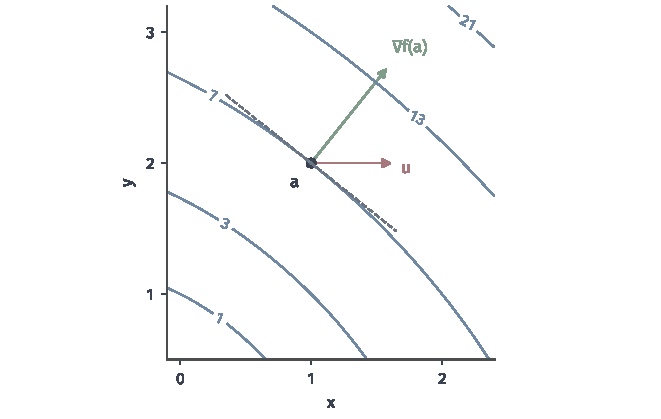
\includegraphics[width=112.0mm]{figures/01-mathematical-preliminaries-upper/01-mathematical-language-combinatorics-analysis-optimization/matplotlib/chapter3-concept-processes/gradient-level-curves.pdf}
 \caption{$f=x^2+xy+y^2$的等值曲线，标注为函数值；基点$a=(1,2)$处$\nabla f=(4,5)^\top$，图中绿箭头按$0.15$倍绘制。灰虚线沿$(5,-4)^\top$，与梯度垂直，因而与经过$a$的等值曲线相切；红箭头为$u=(1,0)^\top$。比较最快上升方向时须先归一化，不能直接比较图中箭头长度。}
 \label{fig:analysis-process-gradient-level-curves}
\end{figure}

\paragraph{偏导数连续给出的充分条件}
如果各坐标的变化率在同一点附近连续，就可以用它们共同控制全部坐标增量。
与上面的必要条件不同，这项条件可以直接保证全微分存在。
\begin{theorem}[偏导数连续与可微性]
\label{thm:multivariable-continuous-partials-sufficient}
设$f:U\to\mathbb R$，$U$开，$\bm a\in U$。若各一阶偏导数在$\bm a$的某个邻域内存在，并在$\bm a$处连续，则$f$在$\bm a$处可微。
\end{theorem}
\begin{proof}
这项条件可以沿坐标逐个改变来核对：把$\bm a$到$\bm a+\bm h$的增量拆成$d$段，
每段只改一个坐标，一元中值定理将该段增量写成相应中间点处的偏导数乘$h_j$。
当$\bm h\to\bm0$时，所有中间点都趋于$\bm a$；偏导连续性因此使
\[
 \begin{aligned}
 &\left|f(\bm a+\bm h)-f(\bm a)-\sum_{j=1}^d\partial_j f(\bm a)h_j\right|\\
 &\qquad\leq \max_j\left|\partial_j f(\bm\xi_j)-\partial_j f(\bm a)\right|
       \sum_{j=1}^d|h_j|
 =o(\lVert\bm h\rVert_2),
 \end{aligned}
\]
其中$\bm\xi_j$是第$j$段的中间点，最后一步用了$\sum_j|h_j|\leq\sqrt d\lVert\bm h\rVert_2$。
这就把各坐标上的变化拼成了同一个有效的全微分。
\end{proof}
偏导数连续只是充分条件。可微仅要求函数增量具有统一的一阶近似，不要求这些系数随基点连续变化。

\paragraph{连续可微函数}
若还希望各点的一阶系数连续变化，就需在一个范围内同时控制偏导数。
实值函数的各一阶偏导数在开集$U$上存在且连续时，称它在$U$上连续可微，记为$C^1(U)$；$C^k(U)$表示直至$k$阶的各偏导数都存在且连续。
刚才的充分条件保证$C^1$函数处处可微，逆向并不成立。

\paragraph{条件之间的蕴含关系}
由必要条件与充分判别，现在可以把这些要求放在一起比较：
\[
 \begin{gathered}
 f\text{在}\bm a\text{的某邻域内连续可微}
 \ \Longrightarrow\ f\text{在}\bm a\text{处可微},\\
 f\text{在}\bm a\text{处可微}
 \ \Longrightarrow\ \text{全部双侧方向导数存在}
 \ \Longrightarrow\ \text{全部偏导数存在}.
 \end{gathered}
\]
第一条已由连续偏导数的充分判别得到，第二条已由必要条件定理证明，最后只须在全部方向中取坐标方向$\bm e_j$。
可微还蕴含连续，并使方向导数关于方向成为同一个线性映射；相应公式已在必要条件中给出。
首项要求一个邻域内偏导数连续，其余各项只约束同一基点；即使要求处处可微，也不能反推连续可微。
一元函数的普通导数存在就等价于可微，多元函数则还须协调多个输入方向，所以上面各条逆命题需要分别检验。

\paragraph{偏导数存在不保证可微}
下面检验蕴含链中的逆命题。先看坐标偏导数：它们只约束坐标切片，并未控制其余方向或路径。
\begin{example}[偏导数存在但不可微]
\label{ex:analysis-partials-not-differentiable}
定义$f:\mathbb{R}^2\to\mathbb{R}$为
\[   f(x,y)=
\begin{cases}     \dfrac{xy}{\sqrt{x^2+y^2}}, & (x,y)\neq(0,0),\\[6pt]     0, & (x,y)=(0,0).
\end{cases} \]
沿两条坐标轴，函数恒为$0$，所以 $\partial f/\partial x(0,0)=\partial f/\partial y(0,0)=0$。若$f$在原点可微， 候选线性部分只能是零映射。可是沿$\bm{h}=(t,t)$，
\[   \frac{|f(t,t)-f(0,0)|}{\lVert(t,t)\rVert_2}   =   \frac{|t|/\sqrt{2}}{\sqrt{2}|t|}   =\frac12, \]
余项与$\lVert\bm{h}\rVert_2$之比不趋于零，故$f$在原点不可微。偏导数只看坐标轴，遗漏了其他接近路径。本例沿每个方向$\bm v=(a,b)$的
正向方向导数都存在，这里只令$t\downarrow0$，得到$ab/\sqrt{a^2+b^2}$（零方向取$0$）；它却不是关于$\bm v$
的线性函数，而且双侧方向导数在$ab\neq0$时不存在。方向极限采用单侧还是双侧，
必须与所用定义一致；本节定义采用双侧极限。
本例还在原点连续，因为$|xy|/\sqrt{x^2+y^2}\leq\sqrt{x^2+y^2}/2$；所以补上连续性也不能反推可微。
\end{example}

\paragraph{全部方向导数存在不保证可微}
从坐标切片扩展到所有固定直线，仍需检查这些变化率能否组成线性映射，以及是否具有统一余项。先看缺少线性性的情形，令
$g(x,y)=x^3/(x^2+y^2)$于非零点，$g(0,0)=0$。
沿$\bm v=(a,b)\neq\bm0$有$D_{\bm v}g(0,0)=a^3/(a^2+b^2)$，
但坐标方向导数给出的候选梯度为$(1,0)^\top$，它对方向$(1,1)^\top$
预测$1$而非实际的$1/2$。这些方向变化率无法拼成一个线性映射。
与前例的单侧方向极限相比，这里直接检验了本节采用的双侧定义。

\begin{example}[所有方向导数为零仍不足以可微]
\label{ex:multivariable-linear-directionals-not-differentiable}
前面的双侧方向导数反例不能组成线性函数。即使补上这一要求，仍需检查统一余项。
在非原点处令$q(x,y)=x^3y/(x^4+y^2)$，并令$q(0,0)=0$。
由$2|x^2y|\leq x^4+y^2$，有$|q(x,y)|\leq|x|/2$，故$q$在原点连续。
对固定方向$(a,b)^\top$，若$b\neq0$，
\[
 \frac{q(ta,tb)}t=\frac{t a^3b}{t^2a^4+b^2}\longrightarrow0;
\]
若$b=0$，差商恒为零。因此所有双侧方向导数都为零，它们也组成零线性映射。
可是沿$\bm h=(t,t^2)^\top$，$q(t,t^2)=t/2$，从而
\[
 \frac{|q(t,t^2)|}{\lVert(t,t^2)\rVert_2}
 =\frac1{2\sqrt{1+t^2}}\longrightarrow\frac12.
\]
候选零映射不能满足全微分的余项条件。方向导数先固定方向再取极限，
全微分则要求对方向随扰动改变的序列也有同一个误差控制。
\end{example}

\paragraph{可微不保证连续可微}
一元函数已经足以否定这个逆命题。在实轴上令$r(0)=0$，$x\neq0$时令$r(x)=x^2\sin(1/x^2)$。
由于$r(h)/h=h\sin(1/h^2)\to0$，有$r'(0)=0$；非零点按运算法则求导得到
\[
 r'(x)=2x\sin(1/x^2)-\frac{2}{x}\cos(1/x^2).
\]
取$x_n=(2\pi n)^{-1/2}$，有$r'(x_n)=-2/x_n\to-\infty$，所以$r'$在$0$处不连续，$r$却处处可微。
在多元情形令$f(\bm x)=r(x_1)$，同样得到处处可微而非连续可微的标量函数。
这个例子还说明可微不保证局部Lipschitz：若原点邻域内有共同Lipschitz常数，那里每个已存在的一元导数都应被这个常数控制，与上述无界导数矛盾。

\paragraph{连续不保证偏导数存在}
反方向也不能从连续性补回微分条件。
例如$f(x,y)=|x|$在整个平面上Lipschitz连续，但原点关于$x$的双侧偏导数不存在，因此在那里不可微。
反向也失败：例~\ref{ex:multivariable-path-limits}中原点置零的$xy/(x^2+y^2)$沿坐标轴恒零，两个偏导数存在，但原点不连续。
因此连续与偏导数存在之间没有一般单向蕴含；可微则能够同时保证二者。

\paragraph{梯度与线性近似的使用条件}
上述反例区分了两种用途：仅有偏导数时，梯度只是坐标变化率排成的向量；确认可微以后，才可用它统一预测增量，并用内积计算任意方向导数。
连续偏导数提供方便的充分判别，却不是必要条件；不满足该判别时，应回到全微分的统一余项定义检查。
后面讨论向量值函数时，将对各个标量输出分量分别检查，再组成Jacobian及复合微分。

\subsubsection{微分的运算法则}

以下$f,g$都在同一开集内定义，并在基点$\bm a$处可微，$c$为固定实数。
将各自的一阶展开相加或相乘，比较线性项与高阶余项，就能逐项得到下面的法则。

\paragraph{和的微分}
函数相加时，一阶近似相加，因此
\[
 \mathrm d(f+g)=\mathrm df+\mathrm dg.
\]
右侧微分在同一基点作用于同一个扰动，两个$o(\lVert\bm h\rVert_2)$余项相加后仍满足可微性要求。

\paragraph{差的微分}
函数相减时，一阶近似相减，因此
\[
 \mathrm d(f-g)=\mathrm df-\mathrm dg.
\]
余项之差仍为$o(\lVert\bm h\rVert_2)$，所以差函数也可微。

\paragraph{数乘的微分}
固定系数只会缩放线性项与余项，故$\mathrm d(cf)=c\,\mathrm df$，包括$c=0$的常函数情形。

\paragraph{积的微分}
展开$(f(\bm a)+\mathrm df(\bm h)+o(\lVert\bm h\rVert_2))(g(\bm a)+\mathrm dg(\bm h)+o(\lVert\bm h\rVert_2))$，保留一次项，得到
\[
 \mathrm d(fg)=g(\bm a)\,\mathrm df+f(\bm a)\,\mathrm dg.
\]
两个线性增量的乘积为$O(\lVert\bm h\rVert_2^2)$，可并入一阶余项，故该计算确实证明乘积可微。

\paragraph{商的微分}
若$g(\bm a)\neq0$，连续性保证邻近分母远离零。一元倒数函数的展开给出$\mathrm d(1/g)=-\mathrm dg/g(\bm a)^2$，再用积法则得到
\[
 \mathrm d(f/g)=\frac{g(\bm a)\,\mathrm df-f(\bm a)\,\mathrm dg}{g(\bm a)^2}.
\]
这里分母非零是定义商函数及估计余项的共同条件。

\paragraph{标量复合函数的微分}
若一元函数$\psi$在$f(\bm a)$处可微，且复合在邻域内有定义，将$f$的增量代入$\psi$的一元展开得到
\[
 \mathrm d(\psi\circ f)=\psi'(f(\bm a))\,\mathrm df.
\]
因为$f(\bm a+\bm h)-f(\bm a)=O(\lVert\bm h\rVert_2)$，外层的一阶余项仍是$o(\lVert\bm h\rVert_2)$。

\paragraph{二次型的微分}
向量自变量的二次型仍是标量函数，有限和的乘积法则可以直接用于它。考虑$q(\bm{x})=\bm{x}^{\top}\bm{A}\bm{x}$，其中 $\bm{A}\in\mathbb{R}^{d\times d}$固定。由乘积法则，
\begin{align*}
  \mathrm{d}q
  &=
  (\mathrm{d}\bm{x})^{\top}\bm{A}\bm{x}
  +\bm{x}^{\top}\bm{A}\,\mathrm{d}\bm{x}\\
  &=
  \bm{x}^{\top}(\bm{A}^{\top}+\bm{A})\,\mathrm{d}\bm{x}.
\end{align*}
因此
\begin{equation}
  \nabla_{\bm{x}}
  \bigl(\bm{x}^{\top}\bm{A}\bm{x}\bigr)
  =
  (\bm{A}+\bm{A}^{\top})\bm{x}.
\label{eq:analysis-quadratic-form-gradient}
\end{equation}
只有当$\bm{A}$对称时才能化为$2\bm{A}\bm{x}$。直接写成$2\bm{A}\bm{x}$会悄然加入对称性条件。

\subsubsection{中值定理与Lipschitz条件}

导数控制一点处的变化；若连接两点的整条线段都在定义域内，可以沿线段使用一元中值定理，得到有限增量的结论。
\begin{theorem}[多元标量函数的中值公式]
\label{thm:multivariable-scalar-mean-value}
设$f$在包含$[\bm x,\bm y]$的开集上可微，$\bm x\neq\bm y$。则存在$\theta\in(0,1)$使
\[
 f(\bm y)-f(\bm x)=\nabla f(\bm x+\theta(\bm y-\bm x))^\top(\bm y-\bm x).
\]
特别地，若沿线段有$\lVert\nabla f\rVert_2\leq L$，则$|f(\bm y)-f(\bm x)|\leq L\lVert\bm y-\bm x\rVert_2$。
\end{theorem}
\begin{proof}
令$\phi(t)=f(\bm x+t(\bm y-\bm x))$。由方向导数公式，$\phi'(t)=\nabla f(\bm x+t(\bm y-\bm x))^\top(\bm y-\bm x)$。
对$\phi$使用一元中值定理得到等式，再用内积不等式得到增量界。
\end{proof}
如果定义域是凸开集且各点梯度范数都不超过同一个有限$L$，任意两点间的线段都在域内，故$f$在全域满足Lipschitz条件。
局部邻域上有这样的界时得到局部Lipschitz条件；不能忽略连接线段是否属于定义域。

特别地，若$f\in C^1(U)$，在每个基点附近取一个包含在$U$内的闭球，连续梯度在球上有界，球内线段也不离开球，故上述估计保证$f$局部Lipschitz。
这不自动给出全域共同常数：实轴上的$x^2$连续可微，但其梯度在全域无界，因而不是全域Lipschitz函数。

\subsection{多元标量函数的高阶微分}
\label{sec:multivariable-curvature-error}

一阶微分记录局部线性变化，高阶微分进一步说明这些系数怎样变化。
下面先把二阶偏导数集中为Hessian矩阵，再用Taylor公式建立二阶近似，最后据此判断驻点的局部极值类型。

\subsubsection{二阶偏导数与Hessian矩阵}

一阶偏导数本身仍是多元标量函数，可以再次求偏导。这里记$f_{x_i x_j}=\partial_j(\partial_i f)$，即先对$x_i$、再对$x_j$求导。
对$f(x,y)=x^2+xy+y^2$，有$f_{xx}=2$、$f_{xy}=f_{yx}=1$、$f_{yy}=2$。一般函数的混合偏导数能否交换，需要额外条件。

\paragraph{混合偏导数的交换}
分别沿两个坐标求导时，先后次序未必自动无关。下面的连续性条件可以把两种次序联系起来。
\begin{theorem}[混合偏导数的交换]
\label{thm:multivariable-mixed-partials}
设$f$在$\bm a$的某个开邻域内有一阶偏导数$\partial_i f,\partial_j f$，混合偏导数$\partial_j\partial_i f,\partial_i\partial_j f$在该邻域存在并在$\bm a$处连续，则
\[
 \partial_j\partial_i f(\bm a)=\partial_i\partial_j f(\bm a).
\]
特别地，$C^2$函数的混合偏导数处处可以交换。
\end{theorem}
\begin{proof}
固定其他坐标，只需讨论二元函数在$(a,b)$处的情形。对小的非零$h,k$考察二阶差分
\[
 \Delta(h,k)=f(a+h,b+k)-f(a+h,b)-f(a,b+k)+f(a,b).
\]
令$\phi(x)=f(x,b+k)-f(x,b)$。先对$\phi$用一元中值定理，再对$y\mapsto f_x(\xi,y)$使用一次中值定理，得到
\[
 \Delta=h[f_x(\xi,b+k)-f_x(\xi,b)]=hk f_{xy}(\xi,\eta),
\]
其中$\xi$在$a,a+h$之间、$\eta$在$b,b+k$之间。先沿$y$方向拆分则得到$\Delta=hk f_{yx}(\xi',\eta')$。
除以$hk$后令$h,k\to0$，各中间点趋于$(a,b)$，连续性使两种混合偏导数在该点相等。
\end{proof}
只有偏导数存在而没有这些连续性条件时，结论可能失败。

\paragraph{Hessian矩阵}
把各偏导数的坐标变化率集中起来，就得到记录二阶信息的矩阵。
它的行、列分别对应先后两次求导的输入坐标。
\begin{definition}[Hessian矩阵]
\label{def:multivariable-hessian}
若$f:U\to\mathbb R$在$\bm x$附近有一阶偏导数，且各$\partial_j\partial_i f(\bm x)$存在，则称
\[
 \nabla^2f(\bm x)=\bigl[\partial_j\partial_i f(\bm x)\bigr]_{i,j=1}^d
\]
为$f$在该点的\term{Hessian矩阵}（Hessian matrix）。
\end{definition}
二阶偏导数存在本身尚不保证一阶导数具有统一的线性近似；二阶可微要求一阶导数映射本身可微。
$C^2$是保证二阶可微的充分条件，且此时Hessian对称。对上面的二次函数，Hessian就是$\begin{bmatrix}2&1\\1&2\end{bmatrix}$。
若$f\in C^2$，沿直线$t\mapsto f(\bm x+t\bm v)$求两次导数，在$t=0$处得到
\[
 \bm v^\top\nabla^2f(\bm x)\bm v
 =\sum_{i=1}^d\sum_{j=1}^d \partial_j\partial_i f(\bm x)v_i v_j.
\]
这个实数二次型衡量沿给定方向的一阶斜率变化。

对二次函数
\[   f(\bm{x})   =   \frac12\bm{x}^{\top}\bm{A}\bm{x}   +\bm{b}^{\top}\bm{x}+c, \]
只有$\bm{A}$的对称部分影响函数值。令 $\bm{H}=(\bm{A}+\bm{A}^{\top})/2$，则 $\nabla f(\bm{x})=\bm{H}\bm{x}+\bm{b}$且 $\nabla^2f(\bm{x})=\bm{H}$。
例如$\bm H=\operatorname{diag}(2,100)$时，方向二次型为$2v_1^2+100v_2^2$，
沿两个坐标方向都向上弯，但第二个方向的二阶变化率是第一个的$50$倍。
若改为$\operatorname{diag}(2,-100)$，两个坐标方向的弯曲方向便相反。
判断曲率需要检查整个二次型，而不是某一个对角元素。

对实对称矩阵$\bm H$，若每个非零$\bm v$都有$\bm v^\top\bm H\bm v>0$，称$\bm H$正定；
若只要求$\bm v^\top\bm H\bm v\geq0$，则称半正定。
把不等号反向得到负定与半负定；若既存在使二次型为正的方向，又存在使它为负的方向，
则称矩阵不定。这些名称分别说明全部方向或某些方向上的曲率符号。



\subsubsection{Taylor公式与局部近似}

把多个坐标同时改变的位移写成一条线段上的参数变化，就能回用一元Taylor公式。
下述公式都针对标量输出，二阶项是一个实数二次型。

一元Taylor定理可沿整条位移线段使用，而基点附近的连续二阶偏导数进一步给出小量形式的余项。
\begin{theorem}[多元标量函数的二阶Taylor公式]
\label{thm:multivariable-second-order-taylor}
设$f\in C^2(U)$，$U\subseteq\mathbb R^d$开，线段$[\bm x,\bm x+\bm h]\subset U$。若$\bm h\neq0$，则存在$\theta\in(0,1)$使
\begin{equation}
 f(\bm x+\bm h)=f(\bm x)+\nabla f(\bm x)^\top\bm h
 +\frac12\bm h^\top\nabla^2f(\bm x+\theta\bm h)\bm h.
\label{eq:analysis-second-order-taylor}
\end{equation}
对固定$\bm x\in U$，当$\bm h\to0$时还有
\begin{equation}
 f(\bm x+\bm h)=f(\bm x)+\nabla f(\bm x)^\top\bm h
 +\frac12\bm h^\top\nabla^2f(\bm x)\bm h+o(\lVert\bm h\rVert_2^2).
\label{eq:analysis-second-order-local-model}
\end{equation}
\end{theorem}
\begin{proof}
令$\phi(t)=f(\bm x+t\bm h)$。由一阶微分公式，$\phi'(t)=\nabla f(\bm x+t\bm h)^\top\bm h$；再对各偏导数沿线段求导，得$\phi''(t)=\bm h^\top\nabla^2f(\bm x+t\bm h)\bm h$。
对$\phi$使用一元Taylor定理即得第一式。矩阵各元素的连续性保证
$\lVert\nabla^2f(\bm x+\theta\bm h)-\nabla^2f(\bm x)\rVert_F\to0$，其中$0<\theta<1$可以随$\bm h$变化。
由$|\bm h^\top\bm B\bm h|\leq\lVert\bm B\rVert_F\lVert\bm h\rVert_2^2$，替换Hessian产生的误差为$o(\lVert\bm h\rVert_2^2)$，得到第二式。上述不等式可对$\sum_{i,j}B_{i,j}h_i h_j$使用有限和的Cauchy--Schwarz不等式验证。
\end{proof}
例如$f(x,y)=e^{x+y}$在原点有函数值$1$、梯度$(1,1)^\top$和各元素均为$1$的Hessian。因此
\[
 e^{h+k}=1+h+k+\frac12(h+k)^2+o(h^2+k^2).
\]
一次项描述切平面，二次项补上沿位移方向的弯曲。

式~\eqref{eq:analysis-second-order-local-model}是局部结论。若要在一个区域内给出统一余项界，还需控制该区域上的Hessian矩阵连续性或Lipschitz常数，不能仅凭一点处的二阶导数。

若希望保留整条位移线段上的曲率，可以直接使用一元Taylor积分余项式~\eqref{eq:analysis-taylor-integral-remainder}。
在同一$C^2$条件下，令$\phi(t)=f(\bm x+t\bm h)$，取该式的$r=1$；刚才已计算出$\phi'$与$\phi''$，代入后得到不挑选中间点的Taylor积分余项：
\[   f(\bm{x}+\bm{h})   =   f(\bm{x})   +\nabla f(\bm{x})^{\top}\bm{h}   +   \int_0^1(1-t)   \bm{h}^{\top}\nabla^2f(\bm{x}+t\bm{h})\bm{h}\,\mathrm{d}t. \]
权重$1-t$说明越靠近位移起点的曲率贡献被累计得越多；该表达式与前面的中间点余项
描述同一有限变化，但保留了整条线段上的曲率信息。

\subsubsection{局部极值的判别}

Taylor公式已经控制线性项以外的误差，因此现在可以将梯度与Hessian的条件转化为原函数的极值结论。
局部极小点是指存在一个相对邻域，使其中所有函数值都不小于基点值；其他点均严格更大时称严格局部极小点，极大点用反向不等式定义。
本小节考察无约束开集内部的点。

\paragraph{局部极值的一阶必要条件}
沿任意方向限制成一元函数后，内部极值点仍必须满足Fermat条件。
这给出与一元导数为零相对应的向量条件。
\begin{theorem}[局部极值的一阶必要条件]
\label{thm:multivariable-extremum-first-order}
设$f$在开集内部点$\bm x^\star$处可微，且该点为局部极小点或局部极大点，则
\begin{equation}
 \nabla f(\bm x^\star)=\bm0.
\label{eq:analysis-first-order-necessary}
\end{equation}
\end{theorem}
\begin{proof}
对每个方向$\bm v$，一元函数$t\mapsto f(\bm x^\star+t\bm v)$在$0$处有局部极值，故导数$\nabla f(\bm x^\star)^\top\bm v=0$。
取各坐标方向，即得全部偏导数为零。
\end{proof}
梯度为零的点称为驻点；驻点未必是极值点。

\paragraph{局部极值的二阶必要条件}
如果邻域内还具有连续二阶偏导数，则任一方向上的一元二阶导数还要具有相应的符号。
\begin{theorem}[局部极值的二阶必要条件]
\label{thm:multivariable-extremum-second-order}
设$f$在$\bm x^\star$附近属于$C^2$。若$\bm x^\star$为内部局部极小点，则
\begin{equation}
 \bm v^\top\nabla^2f(\bm x^\star)\bm v\geq0
 \qquad(\bm v\in\mathbb R^d),
\label{eq:analysis-second-order-necessary}
\end{equation}
即Hessian半正定；内部局部极大点对应Hessian半负定。
\end{theorem}
\begin{proof}
对$t\mapsto f(\bm x^\star+t\bm v)$使用一元极值的二阶必要条件，其二阶导数正是所述二次型。
\end{proof}
必要条件不能单独决定驻点类型。一元函数$x^4$、$-x^4$及$x^3$在$0$处一阶、二阶导数都为零，却分别为极小、极大和非极值；多元函数在二次型退化的方向上同样要检查更高阶项。

\paragraph{驻点的二阶充分条件}
若各非零方向的二次型都有严格符号，Taylor余项便不会改变充分小扰动下的函数增量符号。
\begin{theorem}[驻点的Hessian判别]
\label{thm:multivariable-hessian-classification}
设$f$在$\bm x^\star$附近属于$C^2$，且$\nabla f(\bm x^\star)=0$。
若Hessian正定，则$\bm x^\star$是严格局部极小点；若负定，则为严格局部极大点；若不定，则任意小邻域都存在函数值大于及小于$f(\bm x^\star)$的点。
\end{theorem}
\begin{proof}
正定Hessian矩阵给出更强的充分条件：它要求每个方向都有正曲率，而不只是没有负曲率。
设$f$在$\bm{x}^{\star}$的某个邻域内二阶连续可微，
$\nabla f(\bm{x}^{\star})=\bm{0}$且
$\bm H_\star=\nabla^2f(\bm{x}^{\star})$正定。要把各方向的正曲率变成同一个正下界，
可以在闭有界的单位球面上考察连续函数$\bm v\mapsto\bm v^\top\bm H_\star\bm v$。
由闭有界集上的极值定理，它取到最小值
\[
 \lambda=\min_{\lVert\bm v\rVert_2=1}\bm v^\top\bm H_\star\bm v>0.
\]
正定性保证取到的值仍为正。把任意非零$\bm h$除以其长度，就得到
$\bm h^\top\bm H_\star\bm h\geq\lambda\lVert\bm h\rVert_2^2$。
由Hessian矩阵的连续性，在足够小的球内有
$\lVert\nabla^2f(\bm x)-\bm H_\star\rVert_F\leq\lambda/2$；
Frobenius范数因而把二次型的变化量控制在$(\lambda/2)\lVert\bm h\rVert_2^2$以内，
邻近位置的曲率下界仍至少为$(\lambda/2)\lVert\bm h\rVert_2^2$。
用式~\eqref{eq:analysis-second-order-taylor}
的中间点表达式，即可把这个曲率下界变成函数值下界；具体地，充分靠近时有
\[   f(\bm{x}^{\star}+\bm{h})-f(\bm{x}^{\star})   \geq   \frac{\lambda}{4}\lVert\bm{h}\rVert_2^2>0 \]
对充分小的非零$\bm{h}$成立，故$\bm{x}^{\star}$是严格局部极小点。负定情形给出严格局部极大点。

若驻点处Hessian矩阵不定，分别选取二次型为正和为负的方向。
沿每个固定方向把扰动写成$t\bm v$时，余项为$o(t^2)$，因此充分小的非零$t$不会改变
非零二次项的符号，函数值因而分别增加和减小，该点称为\term{鞍点}（saddle point）。
例如$f(x,y)=x^2-y^2$的原点就是鞍点。
若Hessian矩阵仅半正定或半负定，且在某些非零方向上二次型为零，二阶判据可能没有结论，
必须查看更高阶项或函数的其他结构。上述必要条件还假定点位于无约束开集内部；
边界极小点的梯度可以不为零，受约束问题需要后续章节的可行方向与乘子条件。
\end{proof}


图~\ref{fig:analysis-process-hessian-local-shapes}对照二阶判别可以决定的形状，以及Hessian退化时仍需继续检查的情形。
\begin{figure*}[!htbp]
 \centering
 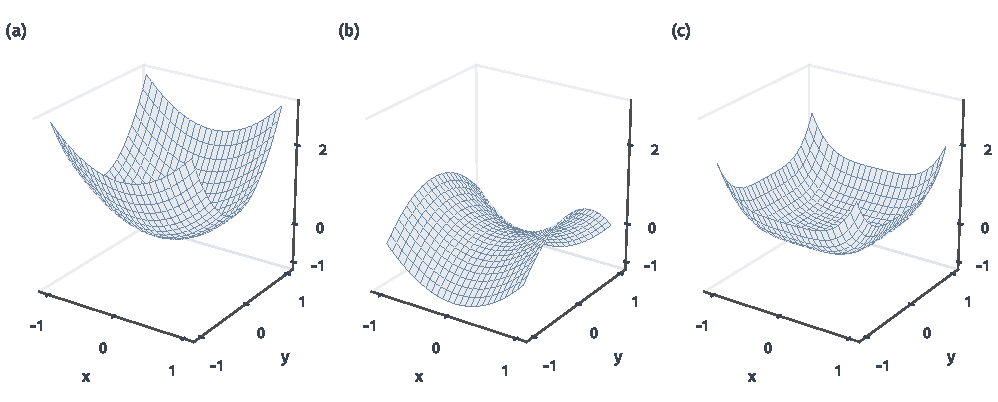
\includegraphics[width=169.0mm]{figures/01-mathematical-preliminaries-upper/01-mathematical-language-combinatorics-analysis-optimization/matplotlib/chapter3-concept-processes/hessian-local-shapes.pdf}
 \caption{同一$[-1,1]^2$范围和纵轴尺度下，三面分别为$x^2+2y^2$、$x^2-y^2$、$x^4+y^4$。原点的Hessian依次为正定、不定、零矩阵；前两者给严格极小与鞍点，第三者虽严格极小却不能由正定判据推出。零Hessian也可能没有极值，例如前述$x^3$，故退化不是一种确定分类。}
 \label{fig:analysis-process-hessian-local-shapes}
\end{figure*}

\FloatBarrier

\subsection{多元向量值函数的微分}

前面每个输入只产生一个实数。现在固定$F:U\subseteq\mathbb R^d\to\mathbb R^m$，同一输入同时产生$m$个输出分量；参数曲线与曲面也是这种映射的特殊情况。
有限个输出可以逐分量检查，但输入仍要整体扰动，不能以坐标切片代替各分量的全微分。

\subsubsection{向量值函数及其极限与连续性}

给出所有输出分量，就确定了整个映射；因此先按输出分量组织其表示。
\begin{definition}[多元向量值函数]
\label{def:multivariable-vector-function}
映射$F:U\subseteq\mathbb R^d\to\mathbb R^m$称为多元向量值函数，写作$F=(F_1,\ldots,F_m)^\top$，其中每个$F_i:U\to\mathbb R$为多元标量函数。
\end{definition}
其极限与连续性使用输出欧氏距离$\lVert F(\bm x)-\bm b\rVert_2$。
对有限个输出，这等价于每个$F_i$的对应极限存在或在同一基点连续，因为
\[
 \max_i|F_i(\bm x)-b_i|\leq\lVert F(\bm x)-\bm b\rVert_2
 \leq\sqrt m\max_i|F_i(\bm x)-b_i|.
\]
这里分解的是输出分量，区别于只沿某些输入坐标检查的切片。

\subsubsection{微分与Jacobian矩阵}

标量输出使用到实数的线性映射，也称线性泛函；向量输出则需要把输入扰动映射为$m$维输出扰动。
有限维线性映射由矩阵表示，矩阵的每一行记录一个输出分量的系数。
\begin{definition}[向量值函数的微分]
\label{def:multivariable-vector-differential}
设$U$开，$F:U\to\mathbb R^m$，$\bm a\in U$。若存在矩阵$\bm J_F(\bm a)\in\mathbb R^{m\times d}$，使
\begin{equation}
 F(\bm a+\bm h)=F(\bm a)+\bm J_F(\bm a)\bm h+o(\lVert\bm h\rVert_2),
\label{eq:analysis-jacobian-linearization}
\end{equation}
则称$F$在$\bm a$处可微，余项按输出欧氏范数理解。
其微分为$\mathrm dF_{\bm a}(\bm h)=\bm J_F(\bm a)\bm h$，其中$\bm J_F$称为\term{Jacobian矩阵}（Jacobian matrix），第$i,j$个元素为$\partial_jF_i$。
\end{definition}
向量值函数可微当且仅当每个输出分量$F_i$可微：正向可从向量余项取分量，反向则将有限个分量的$o(\lVert\bm h\rVert_2)$余项用欧氏范数合并。
因此Jacobian的第$i$行是标量分量梯度$\nabla F_i^\top$；$m=1$时Jacobian是梯度的转置，而不是梯度列向量本身。
$C^k$向量值函数指所有输出分量都属于$C^k$。


图~\ref{fig:analysis-process-jacobian-grid-cell}把向量值映射的线性近似画成小网格块的变化。后面区域换元还会使用这个局部矩阵的行列式。
\begin{figure*}[!htbp]
 \centering
 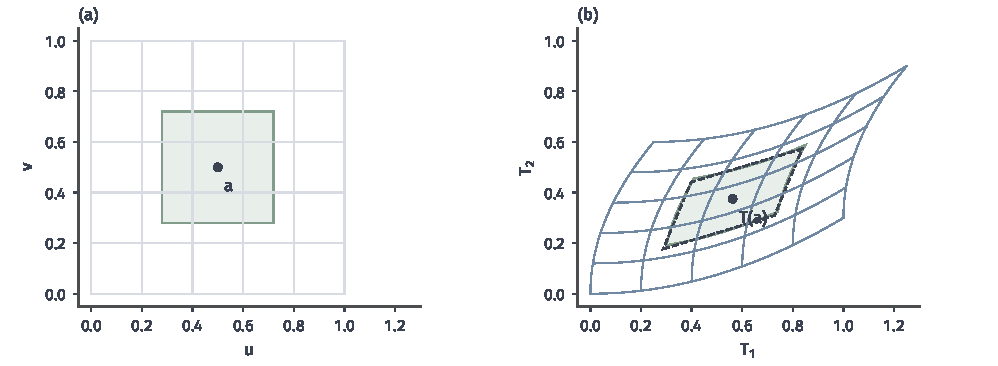
\includegraphics[width=169.0mm]{figures/01-mathematical-preliminaries-upper/01-mathematical-language-combinatorics-analysis-optimization/matplotlib/chapter3-concept-processes/jacobian-grid-cell.pdf}
 \caption{取$T(u,v)=(u+v^2/4,\,0.6v+0.3u^2)$，$a=(0.5,0.5)$。(a) 输入网格及绿色小方块。(b) 非线性像为弯边块，黑虚线为$T(a)+J_T(a)(h,k)^\top$给出的平行四边形；$J_T(a)=\bigl[\begin{smallmatrix}1&0.25\\0.3&0.6\end{smallmatrix}\bigr]$。有限块不与线性像完全重合，缩小扰动后才由可微余项控制差异。}
 \label{fig:analysis-process-jacobian-grid-cell}
\end{figure*}

\paragraph{Jacobian矩阵的计算}
每个输出先按标量函数求偏导，再按行排列，可以核对输入、输出与矩阵形状是否一致。
例如$F(x,y)=(x^2+xy,y^2)^\top$的Jacobian为
\[
 \bm J_F(x,y)=\begin{bmatrix}2x+y&x\\0&2y\end{bmatrix}.
\]
在$(1,2)$处，它把扰动$(h,k)^\top$的一阶影响写成$(4h+k,4k)^\top$。两个输出分别占一行，两个输入分别占一列。

若要把任意实数组变成正数且总和为$1$的权重，可以先取指数再除以共同的总和。
这就是$n$维\term{归一化指数映射}（softmax）。对正整数$n$和
$\bm{z}\in\mathbb{R}^n$，令
\[
  s_i(\bm{z})
  =
  \frac{e^{z_i}}{\sum_{k=1}^n e^{z_k}},
  \qquad i=1,\ldots,n.
\]
记分母为$Z=\sum_k e^{z_k}$。指数函数求导和商法则给出
\[
  \frac{\partial s_i}{\partial z_j}
  =
  \frac{\mathbb{I}\{i=j\}e^{z_i}Z-e^{z_i}e^{z_j}}{Z^2}
  =
  s_i\bigl(\mathbb{I}\{i=j\}-s_j\bigr).
\]
因此整个Jacobian矩阵为
\begin{equation}
  \bm{J}_{\bm{s}}(\bm{z})
  =
  \operatorname{diag}(\bm{s})-\bm{s}\bm{s}^{\top}.
\label{eq:analysis-softmax-jacobian}
\end{equation}
这里$\operatorname{diag}(\bm s)$表示以$s_1,\ldots,s_n$为对角元、其他元素为零的对角矩阵。
对角项$s_i(1-s_i)$描述提高$z_i$对自身分量的影响，非对角项$-s_is_j$
来自共同分母：提高一个坐标会压低其余归一化分量。每行元素之和为零，
这也与给所有$z_i$同时加同一常数不改变输出相符。



\subsubsection{向量值函数的微分运算}
\label{sec:analysis-vector-chain-matrix-calculus}

运算必须先有定义。相同形状的向量输出可以相加、相减和数乘；复合则要求前一映射的输出属于后一映射的定义域。
这里不把没有指定乘法含义的两个向量直接套入标量乘积法则。

\paragraph{和的微分}
若$F,H:U\to\mathbb R^m$在$\bm a$处可微，则逐分量使用和法则，得到
\[
 \bm J_{F+H}(\bm a)=\bm J_F(\bm a)+\bm J_H(\bm a).
\]
相加的输出形状以及两个Jacobian的形状必须分别一致。

\paragraph{差的微分}
在相同条件下，逐分量使用差法则，得到
\[
 \bm J_{F-H}(\bm a)=\bm J_F(\bm a)-\bm J_H(\bm a).
\]

\paragraph{数乘的微分}
对固定实数$c$，逐分量使用数乘法则，得到
\[
 \bm J_{cF}(\bm a)=c\bm J_F(\bm a).
\]

\paragraph{复合函数的链式法则}
前一映射产生的输出扰动，还要经过后一映射的线性响应。
因此复合微分按实际计算顺序组合，Jacobian的乘法次序由输入与输出维度决定。
\begin{theorem}[向量值函数的链式法则]
\label{thm:multivariable-vector-chain-rule}
设$U\subseteq\mathbb R^d$、$V\subseteq\mathbb R^m$开，$F:U\to V$在$\bm a$处可微，$G:V\to\mathbb R^p$在$F(\bm a)$处可微，则$G\circ F$在$\bm a$处可微，且
\begin{equation}
 \bm J_{G\circ F}(\bm a)=\bm J_G(F(\bm a))\bm J_F(\bm a).
\label{eq:analysis-vector-chain-rule}
\end{equation}
\end{theorem}
\begin{proof}
记$\bm A=\bm J_F(\bm a)$、$\bm B=\bm J_G(F(\bm a))$，由$F$可微有$\bm k=F(\bm a+\bm h)-F(\bm a)=\bm A\bm h+o(\lVert\bm h\rVert_2)$，故$\lVert\bm k\rVert_2=O(\lVert\bm h\rVert_2)$。
代入$G$的一阶展开得到$G(F(\bm a)+\bm k)-G(F(\bm a))=\bm B\bm A\bm h+o(\lVert\bm h\rVert_2)$，其中外层余项$o(\lVert\bm k\rVert_2)$也被原扰动尺度控制。
这正是复合函数的可微定义。
\end{proof}
矩阵形状为$(p\times m)(m\times d)=p\times d$，反向相乘往往没有定义。
即使两个次序都有定义，矩阵乘法一般也不交换，不能按标量经验调换因子。这项复合规则称为\term{链式法则}（chain rule）。

\paragraph{标量复合函数的梯度}

前面的外层映射$G$允许向量输出。当$p=1$时，它把中间向量变成一个标量。在优化问题中，
这个标量通常是待最小化的目标值，本书便把此时的$G$记为$\ell$。令
$\bm y=F(\bm x)$，总目标就是$L(\bm x)=\ell(F(\bm x))$；$\ell$只是原复合映射的
最后一层，并没有增加一个未说明的输出。采用列向量梯度，链式法则写成
\[
  \nabla L(\bm x)
  =\bm J_F(\bm x)^\top\nabla\ell(\bm y)\big|_{\bm y=F(\bm x)}.
\]
局部线性映射在前向计算中按$\bm J_F$作用，在标量目标的反向计算中按转置
$\bm J_F^\top$传回。这说明列向量梯度在复合时为何出现Jacobian的转置。


图~\ref{fig:analysis-process-chain-rule-types}把前向的函数复合与反向的梯度传递分开，便于核对转置及维度。
\begin{figure}[!htbp]
 \centering
 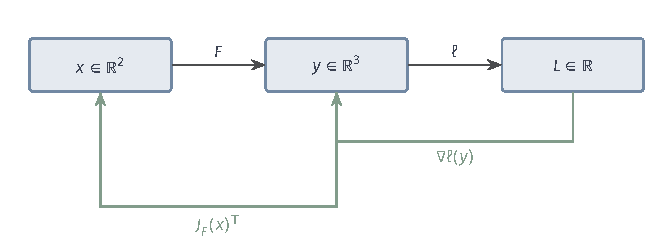
\includegraphics[width=112mm]{figures/01-mathematical-preliminaries-upper/01-mathematical-language-combinatorics-analysis-optimization/tikz/chapter3-concept-processes/chain-rule-types.pdf}
 \caption{上方是$x\in\mathbb R^2$经$F$产生$y\in\mathbb R^3$，再经$\ell$产生标量$L$。下方先得到$\nabla\ell(y)\in\mathbb R^3$，再由$2\times3$矩阵$J_F(x)^\top$传回$\nabla L(x)\in\mathbb R^2$。反向箭头表示梯度的线性传递，不表示对$F$或$\ell$求逆函数。}
 \label{fig:analysis-process-chain-rule-types}
\end{figure}

\begin{example}[从中间向量求回复合目标的梯度]
\label{ex:analysis-chain-rule-calculation}
令
\[
  F(x_1,x_2)=(x_1^2,x_1x_2,x_2)^\top,
  \qquad \ell(\bm y)=\frac12(y_1^2+y_2^2+y_3^2).
\]
$F$从二维输入产生三维中间量，$\ell$再把三维中间量变成一个数。于是
\[
  \bm J_F=\begin{bmatrix}2x_1&0\\x_2&x_1\\0&1\end{bmatrix},
  \qquad \nabla\ell(\bm y)=\bm y.
\]
在$\bm x=(1,2)^\top$处，$\bm y=(1,2,2)^\top$，链式法则给出
\[
  \nabla L(1,2)
  =\begin{bmatrix}2&2&0\\0&1&1\end{bmatrix}
    \begin{bmatrix}1\\2\\2\end{bmatrix}
  =\begin{bmatrix}6\\4\end{bmatrix}.
\]
也可以把复合函数直接展开为
$L(x_1,x_2)=\tfrac12(x_1^4+x_1^2x_2^2+x_2^2)$，求偏导得到
$\nabla L=(2x_1^3+x_1x_2^2,\,x_1^2x_2+x_2)^\top$，在同一点仍为$(6,4)^\top$。
两种计算处理同一个目标；链式形式保留了中间映射，可分别复用各层的导数。
矩阵形状$(2\times3)(3\times1)=2\times1$也核对了梯度传递的次序。
\end{example}


\subsubsection{向量增量的中值估计}

各输出分量的一元中值位置可能不同，不能保证有一个共同位置代表整个向量增量。
可以改为控制增量的范数，用线性映射的最大放大倍数估计有限变化。

\paragraph{算子范数}

对向量输出，用线性映射的最大放大倍数替代标量导数的绝对值。
\begin{definition}[欧氏诱导算子范数]
\label{def:analysis-induced-operator-norm}
对矩阵
$\bm{A}\in\mathbb{R}^{s\times r}$，由欧氏范数\term{诱导的算子范数}
（induced operator norm）定义为
\[
  \lVert\bm{A}\rVert_{\mathrm{op}}
  =
  \sup_{\bm{h}\neq\bm{0}}
  \frac{\lVert\bm{A}\bm{h}\rVert_2}{\lVert\bm{h}\rVert_2}
  =
  \sup_{\lVert\bm{h}\rVert_2=1}\lVert\bm{A}\bm{h}\rVert_2.
\]
\end{definition}
它表示线性映射对向量长度的最大放大倍数，定义立即给出
$\lVert\bm{A}\bm{h}\rVert_2
\leq\lVert\bm{A}\rVert_{\mathrm{op}}\lVert\bm{h}\rVert_2$。
例如$\bm A=\operatorname{diag}(2,1)$把第一坐标放大两倍、第二坐标保持不变，
故$\lVert\bm A\rVert_{\mathrm{op}}=2$；最大放大由第一坐标方向达到。

在含整条线段的开邻域内连续可微时，下面的范数界不要求各分量共用一个中值点。
\begin{theorem}[向量值函数的中值估计]
\label{thm:multivariable-vector-mean-value}
设$U\subseteq\mathbb R^r$开，$G:U\to\mathbb R^s$连续可微，且$[\bm y',\bm y]\subset U$，则
\begin{equation}
  \begin{aligned}
  \lVert G(\bm{y})-G(\bm{y}')\rVert_2
  &\leq
  \sup_{0\leq t\leq1}
  \left\lVert
    \bm{D}G\bigl(\bm{y}'+t(\bm{y}-\bm{y}')\bigr)
  \right\rVert_{\mathrm{op}}
  \lVert\bm{y}-\bm{y}'\rVert_2.
  \end{aligned}
\label{eq:analysis-operator-mean-value-bound}
\end{equation}
其中$\bm DG=\bm J_G$，即$G$的Jacobian矩阵。
\end{theorem}
\begin{proof}
这个向量上界无需预先使用积分公式。若$\bm u=G(\bm y)-G(\bm y')\neq\bm0$，
取单位向量$\bm v=\bm u/\lVert\bm u\rVert_2$，并沿线段定义标量函数
$\phi(t)=\bm v^\top G(\bm y'+t(\bm y-\bm y'))$。
中值定理给出某个$\tau\in(0,1)$，使
\[
 \lVert\bm u\rVert_2
 =\phi(1)-\phi(0)
 =\bm v^\top\bm DG(\bm y'+\tau(\bm y-\bm y'))(\bm y-\bm y').
\]
对右侧使用欧氏内积与算子范数的上界便得到式~\eqref{eq:analysis-operator-mean-value-bound}；
$\bm u=\bm0$时该界直接成立。
\end{proof}
若定义域为凸开集，且Jacobian的算子范数在全域不超过同一个有限$L$，则$G$为Lipschitz连续；局部球上的界给出局部版本。
特别地，若在某邻域内$L<1$，映射严格缩小任意两点间的距离。后面的隐函数构造将使用这一条件和几何尾和控制迭代。

\subsection{矩阵自变量函数的微分}

本小节的定义域$\mathcal U$均为全矩阵空间$\mathbb R^{m\times n}$中的开集，基点$\bm X\in\mathcal U$；因此全部充分小的同形扰动都允许使用。矩阵$\bm X$可以看成$mn$个实数坐标组成的输入；保留矩阵形状，能让乘法次序与迹的结构更清楚。
输出仍须分别说明：$f(\bm X)$为标量时使用矩阵梯度，$\Phi(\bm X)$为矩阵时则使用矩阵到矩阵的线性微分。

\subsubsection{矩阵标量函数的微分与梯度}

第~\ref{sec:prelim-matrix-trace}节已定义Frobenius内积与范数，满足$\langle\bm A,\bm B\rangle_F=\operatorname{tr}(\bm A^\top\bm B)$。
现在用该范数度量输入扰动，用该内积表示标量输出的一阶变化。
\begin{definition}[矩阵标量函数的梯度]
\label{def:multivariable-matrix-scalar-gradient}
设$f:\mathcal U\to\mathbb R$。若它在矩阵$\bm X$处满足
\[
 f(\bm X+\bm H)=f(\bm X)+\mathrm df_{\bm X}(\bm H)+o(\lVert\bm H\rVert_F),
\]
其中$\mathrm df_{\bm X}$为矩阵到实数的线性映射，则称$f$在该点可微。
唯一满足
\begin{equation}
 \mathrm df_{\bm X}(\bm H)=\langle\nabla_{\bm X}f,\bm H\rangle_F
 =\operatorname{tr}\bigl((\nabla_{\bm X}f)^\top\bm H\bigr)
\label{eq:analysis-matrix-gradient-definition}
\end{equation}
的同形矩阵$\nabla_{\bm X}f\in\mathbb R^{m\times n}$称为矩阵梯度。
\end{definition}
它的各元素是对相应矩阵坐标的偏导数，唯一性可逐个取只有一个非零元素的扰动检验。
计算时先用乘积法则展开微分，再利用迹的循环移位将扰动移到末端。例如乘积形状相容时，
\[
 \operatorname{tr}(\bm A\bm B)=\operatorname{tr}(\bm B\bm A),\qquad
 \operatorname{tr}(\bm A\bm B\bm C)=\operatorname{tr}(\bm B\bm C\bm A).
\]
这里循环移动的是整个因子，不能任意交换相邻矩阵。矩阵梯度的唯一性使用了全部矩阵方向；若把定义域限制在对称矩阵等子空间上，还需另行说明所用的内积与允许方向。

\paragraph{迹函数的微分}
线性迹函数已经符合定义，可以直接读出梯度。
对固定的$\bm{A}\in\mathbb{R}^{m\times n}$，令 $f(\bm{X})=\operatorname{tr}(\bm{A}^{\top}\bm{X})$。它的微分已经符合式
\eqref{eq:analysis-matrix-gradient-definition}，所以
\begin{equation}
  \nabla_{\bm{X}}\operatorname{tr}(\bm{A}^{\top}\bm{X})
  =\bm{A}.
\label{eq:analysis-trace-linear-gradient}
\end{equation}
这个简单关系常用于从迹表达式中读出梯度。

\paragraph{行列式的微分}
行列式把方阵映为一个实数，可以通过有限多项式展开来求微分。下面先在可逆矩阵处计算，便于使用行列式的乘法公式。
第~\ref{sec:prelim-determinants}节的有限多项式表达式可用来直接识别一阶项。
先设$\bm X\in\mathbb R^{d\times d}$可逆。
计算它的一阶变化，先把方向扰动$\bm H$从行列式中分离出来：
\[
 \det(\bm X+t\bm H)=\det(\bm X)\det(\bm I+t\bm X^{-1}\bm H).
\]
对固定矩阵$\bm B$，行列式的排列展开给出
$\det(\bm I+t\bm B)=1+t\operatorname{tr}(\bm B)+O(t^2)$。
其中一次项只能从恒等排列的一个对角位置选取$tB_{i,i}$，其余位置选$1$；
非恒等排列至少改变两个位置，因此只贡献二次及以上项。
行列式是有限多项式，故在固定$\bm X$附近，对任意小矩阵扰动$\bm H$，
同一展开中的二阶及更高阶项也统一为$O(\lVert\bm H\rVert_F^2)$；这保证得到的是全微分，而不只是固定方向上的导数。
代入$\bm B=\bm X^{-1}\bm H$，便得到Jacobi行列式公式的一阶形式
\[   \mathrm{d}\det\bm{X}   =   \det(\bm{X})\operatorname{tr}   (\bm{X}^{-1}\mathrm{d}\bm{X}). \]
\paragraph{对数行列式的微分}
实数对数还要求$\det\bm X>0$，它在该开集上与行列式复合。对上面的微分应用标量对数的链式法则，得到
\begin{equation}
  \mathrm{d}\log\det\bm{X}
  =
  \operatorname{tr}(\bm{X}^{-1}\mathrm{d}\bm{X}),
  \qquad
  \nabla_{\bm{X}}\log\det\bm{X}
  =
  \bm{X}^{-\top}.
\label{eq:analysis-logdet-gradient}
\end{equation}
若$\bm X$还对称，则$\bm{X}^{-\top}=\bm{X}^{-1}$；一般情形应保留转置。
这些计算都先找出扰动的一阶项，再用迹内积读出梯度；乘积次序与行列式展开决定了哪些变形成立。

\subsubsection{矩阵值函数的微分}

求逆映射的输出与输入都是方阵，不能用一个同形梯度表示全部输出的一阶变化。
若$\Phi:\mathcal U\to\mathbb R^{r\times s}$满足$\Phi(\bm X+\bm H)=\Phi(\bm X)+A(\bm H)+o(\lVert\bm H\rVert_F)$，其中$A$为矩阵空间之间的线性映射、余项按输出Frobenius范数度量，则$A$为其微分。
这就是前面的向量值可微性按矩阵形状重排，不能把不同输出元素共用一个标量系数。

\paragraph{逆矩阵的微分}
逆矩阵与行列式非零的关系在第~\ref{sec:prelim-inverse-matrices}节及第~\ref{sec:prelim-determinants}节已经建立。
这里先确认可微，再对乘法恒等式取微分。
第~\ref{sec:prelim-determinants}节的代数余子式公式把逆矩阵的各元素写成多项式与$\det\bm X$的比。
因此，在$\det\bm X\neq0$的开集内，每个元素都是连续可微函数，逆映射也连续可微。
确认可微性后，对恒等式$\bm{X}\bm{X}^{-1}=\bm{I}$取微分可得
\[   (\mathrm{d}\bm{X})\bm{X}^{-1}   +\bm{X}\,\mathrm{d}(\bm{X}^{-1})=\bm{0}. \]
左乘$\bm{X}^{-1}$后得到
\begin{equation}
  \mathrm{d}(\bm{X}^{-1})
  =
  -\bm{X}^{-1}(\mathrm{d}\bm{X})\bm{X}^{-1}.
\label{eq:analysis-inverse-differential}
\end{equation}
两个$\bm{X}^{-1}$位于扰动两侧，不能合并成 $-\bm{X}^{-2}\mathrm{d}\bm{X}$，因为$\mathrm{d}\bm{X}$未必与$\bm{X}^{-1}$交换。



\begin{example}[逆矩阵微分中的乘法次序]
\label{ex:analysis-noncommuting-inverse-differential}
取$\bm X=\operatorname{diag}(2,1)$，扰动方向
$\bm E=\begin{bmatrix}0&1\\1&0\end{bmatrix}$。沿$\bm X+t\bm E$求逆矩阵的导数为
\[
 -\bm X^{-1}\bm E\bm X^{-1}
 =\begin{bmatrix}0&-1/2\\-1/2&0\end{bmatrix}.
\]
若照搬标量规则而写成$-\bm X^{-2}\bm E$，会得到
$\begin{bmatrix}0&-1/4\\-1&0\end{bmatrix}$，连对称性都丢失。
原路径在$0$附近由对称可逆矩阵组成，其逆与导数也应对称；这一结构检查能直接发现错误。
矩阵变量沿给定方向微分时，夹在两侧的逆矩阵不能随意移到同一侧。
\end{example}

\subsection{隐函数与反函数}
\label{sec:analysis-implicit-parameter-integral}

前面把已给定的映射作微分；这里改变问题，先给定一组方程，再判断它是否在基点附近确定唯一的函数。
一般方程组采用向量值映射，待解变量与方程数量的对应关系决定哪个Jacobian必须可逆。

\subsubsection{隐函数的定义}

显式函数直接给出输出，例如$y=\sqrt x$。关系$F(x,y)=0$则没有直接选定一个输出。
若在一点$(a,b)$附近存在函数$y=\varphi(x)$，使这些局部解恰好满足$y=\varphi(x)$，就称方程在此确定了一个\term{隐函数}（implicit function）。
隐函数研究的第一步是局部解分支存在且唯一，然后才是对这条分支求导。

例如方程$y^2-x=0$在$x>0$时有正、负两支解。固定其中一个非零解后，可以在它附近选出唯一分支；但在$(0,0)$，两支相交，负$x$侧还没有实数解，因此不存在覆盖$0$的开区间上的可微解函数。此处$\partial F/\partial y=2y=0$，恰好失去了下面定理要求的可逆性。这个例子说明，局部选解既要指定起始解，也要核对关于待解变量的导数。

图~\ref{fig:vol1-add-implicit-branches}说明“局部唯一”怎样排除另一支解。在$(1,1)$附近只保留正支即可；在原点处，两支相交且负$x$没有实数解，不能沿用同样的局部可微选解。
\begin{figure}[!htb]
  \centering
  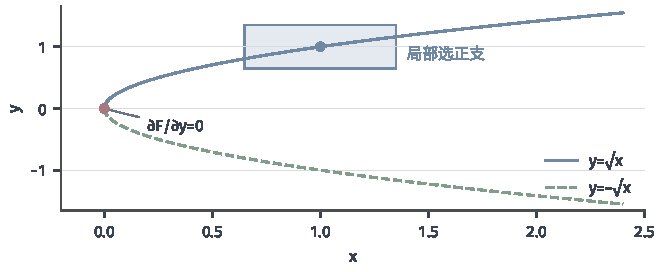
\includegraphics[width=112mm]{figures/01-mathematical-preliminaries-upper/01-mathematical-language-combinatorics-analysis-optimization/matplotlib/comprehension-additions/implicit-branches.pdf}
  \caption{方程$F(x,y)=y^2-x=0$的两支实数解。浅蓝矩形围住$(1,1)$，在该矩形内每个允许的$x$只有正支解，且$F_y=2y\neq0$；红点处$F_y=0$，两支相交。图的两个根都属于同一方程，选定起始解与邻域才确定隐函数分支。}
  \label{fig:vol1-add-implicit-branches}
\end{figure}
\FloatBarrier


\subsubsection{隐函数的存在、唯一性与微分}

下面的充分条件先保证局部解存在且唯一，再保证解随参数连续可微。
可逆性只要求待解变量对应的方阵Jacobian可逆，并非要求整个带参数映射为方阵。
\begin{theorem}[隐函数定理]
\label{thm:analysis-implicit-function}
设$F:\mathbb{R}^p\times\mathbb{R}^m\to\mathbb{R}^m$在 $(\bm{a},\bm{b})$的某个开邻域内连续可微， $F(\bm{a},\bm{b})=\bm{0}$，并且关于待解变量的Jacobian矩阵 \[   \bm{D}_{\bm{y}}F(\bm{a},\bm{b})   \in\mathbb{R}^{m\times m} \]
可逆。则存在$\bm{a}$与$\bm{b}$的邻域$U,V$，以及唯一的连续可微函数
$\varphi:U\to V$，使$\varphi(\bm{a})=\bm{b}$，并且对所有
$(\bm{x},\bm{y})\in U\times V$都有
\[
  F(\bm{x},\bm{y})=\bm{0}
  \quad\Longleftrightarrow\quad
  \bm{y}=\varphi(\bm{x}).
\]
其Jacobian矩阵满足
\begin{equation}
  \bm{D}\varphi(\bm{x})
  =
  -
  \bigl[\bm{D}_{\bm{y}}F(\bm{x},\varphi(\bm{x}))\bigr]^{-1}
  \bm{D}_{\bm{x}}F(\bm{x},\varphi(\bm{x})).
\label{eq:analysis-implicit-derivative}
\end{equation}
\end{theorem}

证明将方程改写为局部压缩迭代，再分别检查统一压缩、自映射与解的可微性；形式求导不能替代这些存在性步骤。
\begin{proof}
为证明定理~\ref{thm:analysis-implicit-function}的存在性，先把方程改写为局部压缩迭代。记
\[   \bm{A}   =   \bm{D}_{\bm{y}}F(\bm{a},\bm{b}),   \qquad   T_{\bm{x}}(\bm{y})   =   \bm{y}-\bm{A}^{-1}F(\bm{x},\bm{y}). \]
$F(\bm{x},\bm{y})=\bm{0}$当且仅当$T_{\bm{x}}(\bm{y})=\bm{y}$，即$\bm y$是更新后保持不变的点，称为不动点。并且
\[   \bm{D}_{\bm{y}}T_{\bm{x}}(\bm{y})   =   \bm{I}   -   \bm{A}^{-1}\bm{D}_{\bm{y}}F(\bm{x},\bm{y}), \]
它在$(\bm{a},\bm{b})$处为零。由导数连续性，可以选择闭球 $B=\{\bm{y}:\lVert\bm{y}-\bm{b}\rVert_2\leq r\}$和$\bm{a}$的邻域$U$，使
\begin{equation}
  \sup_{\bm{x}\in U,\,\bm{y}\in B}
  \left\lVert
    \bm{D}_{\bm{y}}T_{\bm{x}}(\bm{y})
  \right\rVert_{\mathrm{op}}
  \leq q<1.
\label{eq:analysis-ift-uniform-contraction}
\end{equation}
沿$\bm{y}$方向使用式~\eqref{eq:analysis-operator-mean-value-bound}可知，每个
$T_{\bm{x}}$都把$B$内任意两点之间的距离缩小到原来的至多$q$倍。

还必须核对自映射。因为$T_{\bm{a}}(\bm{b})=\bm{b}$且$T_{\bm{x}}(\bm{b})$关于 $\bm{x}$连续，可进一步缩小$U$，使
\[   \lVert T_{\bm{x}}(\bm{b})-\bm{b}\rVert_2   \leq\frac{1-q}{2}r. \]
于是对$\bm{y}\in B$，
\[
  \lVert T_{\bm{x}}(\bm{y})-\bm{b}\rVert_2
  \leq
  q\lVert\bm{y}-\bm{b}\rVert_2+\frac{1-q}{2}r
  \leq
  \frac{1+q}{2}r
  <r.
\]
所以$T_{\bm{x}}(B)$包含在$B$的内部$V$中。
固定$\bm x\in U$，从$\bm y_0=\bm b$出发，令$\bm y_{n+1}=T_{\bm x}(\bm y_n)$。
所有迭代项都留在$B$内，相邻差满足
$\lVert\bm y_{n+1}-\bm y_n\rVert_2\leq q^n\lVert\bm y_1-\bm y_0\rVert_2$。
增大$q$仍保留这个上界，因而可设$0<q<1$。对$m>n$，几何和给出
\[
 \lVert\bm y_m-\bm y_n\rVert_2
 \leq\sum_{j=n}^{m-1}\lVert\bm y_{j+1}-\bm y_j\rVert_2
 \leq\frac{q^n}{1-q}\lVert\bm y_1-\bm y_0\rVert_2\longrightarrow0.
\]
每个坐标都是实柯西列，所以该序列在有限维欧氏空间中收敛；闭性使极限仍在$B$内。
$T_{\bm x}$连续，令$n\to\infty$可得极限$\varphi(\bm x)$满足
$T_{\bm x}(\varphi(\bm x))=\varphi(\bm x)$，而映射的内部包含关系使它属于$V$。
若另有不动点$\bm z$，则
$\lVert\bm z-\varphi(\bm x)\rVert_2\leq q\lVert\bm z-\varphi(\bm x)\rVert_2$，
由$q<1$只能有$\bm z=\varphi(\bm x)$，所以这个不动点唯一。若
$(\bm{x},\bm{y})\in U\times V$且$F(\bm{x},\bm{y})=\bm{0}$，则$\bm{y}\in B$也是
$T_{\bm{x}}$的不动点，唯一性迫使$\bm{y}=\varphi(\bm{x})$。这证明了定理所述的局部
存在与零点集合的逐点唯一性。

还需说明所得解随参数连续可微。把$U$进一步缩小为开球，并使
$\overline U\times B$包含在原定义域内；这个集合闭且有界，关于$\bm x$的导数各分量连续，
故有统一范数上界$L$。对$\bm x,\bm x'\in U$，
两点间的线段仍在$U$内，式~\eqref{eq:analysis-operator-mean-value-bound}
可用于$T_{\bm x}(\bm y)$的参数变化。利用两个不动点关系，
\[   \lVert\varphi(\bm{x})-\varphi(\bm{x}')\rVert_2   \leq   q\lVert\varphi(\bm{x})-\varphi(\bm{x}')\rVert_2   +L\lVert\bm{x}-\bm{x}'\rVert_2, \]
移项得到$\lVert\varphi(\bm x)-\varphi(\bm x')\rVert_2
\leq L\lVert\bm x-\bm x'\rVert_2/(1-q)$，
故$\varphi$局部Lipschitz连续。令 $\bm{h}\to\bm{0}$并记 $\bm{k}=\varphi(\bm{x}+\bm{h})-\varphi(\bm{x})$，前述界给出 $\lVert\bm{k}\rVert_2=O(\lVert\bm{h}\rVert_2)$。对恒等式
\[   F(\bm{x}+\bm{h},\varphi(\bm{x})+\bm{k})   -   F(\bm{x},\varphi(\bm{x}))   =   \bm{0} \]
作一阶展开，得到
\[   \bm{D}_{\bm{x}}F\,\bm{h}   +   \bm{D}_{\bm{y}}F\,\bm{k}   +   o(\lVert\bm{h}\rVert_2)   =   \bm{0}. \]
展开中的Jacobian均在$(\bm x,\varphi(\bm x))$处取值，联合扰动的余项
$o(\lVert(\bm h,\bm k)\rVert_2)$因$\lVert\bm k\rVert_2=O(\lVert\bm h\rVert_2)$
成为$o(\lVert\bm h\rVert_2)$。
基点的$\det\bm A\neq0$，行列式又是矩阵元素的连续函数，
所以邻域足够小时$\bm D_{\bm y}F$仍可逆。于是
\[   \bm{k}   =   -   (\bm{D}_{\bm{y}}F)^{-1}   \bm{D}_{\bm{x}}F\,\bm{h}   +   o(\lVert\bm{h}\rVert_2). \]
这证明$\varphi$可微并给出式~\eqref{eq:analysis-implicit-derivative}；各Jacobian矩阵连续又保证$\bm{D}\varphi$连续。至此，隐函数定理中的存在、局部唯一与导数公式都已得到说明。证明中特别核对了自映射和统一压缩条件，只有形式上的固定点改写并不足够。
\end{proof}

\paragraph{隐函数的导数}

定理的证明已同时建立解分支的存在、唯一性、可微性及式~\eqref{eq:analysis-implicit-derivative}。计算时只需在选定分支上代入两个Jacobian；下面用最初的方程核对正、负分支各自的变化率。

\begin{example}[隐函数分支的导数]
设$F(x,y)=y^2-x$，在$(1,1)$处有$F=0$、$F_y=2\neq0$。
隐函数定理保证$(1,1)$附近的解可以唯一写成$y=\varphi(x)$，且
\[
 \varphi'(x)=-\frac{F_x(x,\varphi(x))}{F_y(x,\varphi(x))}
 =\frac1{2\varphi(x)},\qquad \varphi'(1)=\frac12.
\]
直接选正支$\varphi(x)=\sqrt x$，求导同样得到$1/(2\sqrt x)$。
若在$(1,-1)$附近选负支，导数则为$-1/2$；起始解不同，所追踪的函数也不同。
\end{example}


\subsubsection{反函数的存在与微分}

反求一个向量值映射的输入，可以看成以输出为参数的一组方程，从而回用隐函数的结论。
以下只保证邻域之间的逆，不预先断言整个定义域上的映射单射。
\begin{theorem}[局部反函数定理]
\label{thm:multivariable-inverse-function}
设$U\subseteq\mathbb R^d$开，$G:U\to\mathbb R^d$连续可微，$\bm a\in U$，且$\bm J_G(\bm a)$可逆。
则存在$\bm a$的开邻域$U_0$与$G(\bm a)$的开邻域$V_0$，使$G:U_0\to V_0$为双射，逆映射连续可微，并满足
\[
 \bm J_{G^{-1}}(G(\bm x))=[\bm J_G(\bm x)]^{-1}
 \qquad(\bm x\in U_0).
\]
\end{theorem}
\begin{proof}
以输出$\bm y$为参数、原输入$\bm x$为待解变量，令$H(\bm y,\bm x)=G(\bm x)-\bm y$。
在$(G(\bm a),\bm a)$处，关于$\bm x$的Jacobian就是可逆的$\bm J_G(\bm a)$。隐函数定理给出开邻域$V_0$、$W$以及$C^1$映射$\varphi:V_0\to W$，使
\[
 G(\bm x)=\bm y\quad\Longleftrightarrow\quad\bm x=\varphi(\bm y)
 \qquad(\bm y\in V_0,\ \bm x\in W).
\]
将$W$缩小并重新选取$V_0$，可使$W\subset U$且$\bm J_G$在$W$内均可逆。
令$U_0=W\cap G^{-1}(V_0)$，它因$G$连续而为包含$\bm a$的开集。
每个$\bm y\in V_0$都有$G(\varphi(\bm y))=\bm y$，故$\varphi(\bm y)\in U_0$；反之，每个$\bm x\in U_0$都由上述唯一性满足$\varphi(G(\bm x))=\bm x$。
因此$G:U_0\to V_0$为双射，逆就是$C^1$映射$\varphi$。
对$G(\varphi(\bm y))=\bm y$使用链式法则，得到$\bm J_G(\varphi(\bm y))\bm J_\varphi(\bm y)=\bm I$，左乘逆矩阵便得到所述公式。
\end{proof}

\paragraph{局部可逆与整体单射}

Jacobian处处可逆仍不保证整个定义域上单射。例如
$g(u,v)=(e^u\cos v,e^u\sin v)^\top$的Jacobian行列式为$e^{2u}>0$，
但$v$与$v+2\pi$给出同一输出。它在每一点附近可以反求，整个平面上的输入却会重复覆盖输出。
反过来，存在连续逆也不保证逆可微：一元函数$x\mapsto x^3$全局单射，
其逆在$0$处没有有限导数。使用局部逆定理时，需要逐项检查邻域、可微性和可逆Jacobian。

\FloatBarrier

\section{区域积分}
\label{sec:multivariable-region-integration}

平面薄片的质量由面密度在整块区域上的累计给出，空间物体的质量则要累计体密度。
这里的被积对象都是多元标量函数$f:D\subseteq\mathbb R^d\to\mathbb R$：输入有多个坐标，每个位置只输出一个待累计的数。
一元积分的长度权重需要相应换成$d$维勒贝格测度，积分的简单函数构造和绝对可积要求则继续适用。

实际计算还要回答两个问题：何时能逐个坐标做一元积分，何时能改用另一套坐标？
前者需要非负性或绝对可积性来保证累次积分成立，后者需要坐标变换的Jacobian来校正体积。
坐标变换是一个向量值映射，不是这里的标量被积函数。
最后再把被积函数看成依赖参数的一族标量函数，讨论积分的连续性和求导。切片与坐标计算可参考\scite{math-openstax-calculus3}。

\subsection{多维测度与乘积测度}
\label{sec:comb-multidimensional-product-measure}

实轴上的测量建立以后，还需要测量成对或多坐标对象构成的集合。
有限集合满足$|A\times B|=|A||B|$，长方形满足“面积等于两边长度之积”，这提示我们用各方向测度的乘积测量矩形。
下面先把区间覆盖构造直接推广到多维，再说明一般测度空间中的乘积构造；两者会在多维长度、面积和体积上衔接。

\subsubsection{多维勒贝格测度}

\paragraph{坐标盒}

$d$维坐标盒是区间的笛卡尔积，例如
\[
 Q=\prod_{i=1}^d(a_i,b_i),\qquad a_i<b_i.
\]
它的体积为$\prod_i(b_i-a_i)$。例如$(0,2)\times(0,3)$的面积为$6$。
所有开盒生成$\mathbb R^d$上的Borel $\sigma$代数$\mathcal B(\mathbb R^d)$。

\paragraph{多维勒贝格测度}

一维外测度通过可数区间覆盖比较总长度。把覆盖对象改为开盒、长度改为体积，就能用同一思路测量$\mathbb R^d$中的集合：
\[
 m_d^*(E)=\inf_{\substack{E\subseteq\bigcup_{n=1}^{\infty}Q_n\\
 Q_n\text{为开坐标盒}}}\sum_{n=1}^{\infty}\operatorname{vol}(Q_n).
\]
下确界取遍$E$的所有可数开盒覆盖。再要求集合$A$对每个测试集合$E\subseteq\mathbb R^d$满足
$m_d^*(E)=m_d^*(E\cap A)+m_d^*(E\setminus A)$，就得到勒贝格可测集族$\mathcal L_d$。
外测度限制在这个$\sigma$代数上，给出完备的$d$维勒贝格测度$m_d$，其中$m_1=m$。
前面关于外测度、可测分割和可数可加性的论证只需将区间换成盒，即可按同样步骤推广；$m_d$为坐标盒赋予边长之积。

每个欧氏开集都是其中有理端点开盒的可数并，所以开盒生成的Borel范围包含全部开集。
因此$\mathcal B(\mathbb R^d)\subseteq\mathcal L_d$；勒贝格范围还包含Borel零测集的全部子集。

\subsubsection{乘积测度}

多维勒贝格测度使用欧氏空间中的坐标盒；一般的乘积测度则从任意两个测度空间出发，以$A\times B$作为基本矩形。
为保证下面的乘积测度存在且唯一，先说明所采用的$\sigma$有限条件：允许总量无限，但空间能够被可数个有限测度部分覆盖。

\paragraph{$\sigma$有限测度}

若整个空间测度有限，就称为有限测度。更一般地，可要求空间由可数个有限测度集合覆盖。
\begin{definition}[$\sigma$有限测度]
\label{def:analysis-sigma-finite-measure}
若存在$E_n\in\mathcal A$，使$X=\bigcup_{n=1}^{\infty}E_n$且每个$n$都满足$\mu(E_n)<\infty$，称测度空间$(X,\mathcal A,\mu)$为\term{$\sigma$有限}（sigma-finite）的。
\end{definition}

例如$\mathbb R=\bigcup_n[-n,n]$，每段长度有限，所以勒贝格测度$\sigma$有限。
有限集合上的计数测度是有限测度；可数无限集合上的计数测度虽总量无限，仍$\sigma$有限。
不可数集合上的计数测度则不$\sigma$有限，因为有限测度子集只能有限，可数个这样的集合仍不能覆盖不可数集。

\paragraph{乘积$\sigma$代数}

矩形适合规定基本赋值，但矩形的并或补一般不再是一个矩形，因此不能只把矩形本身当作全部可测集合。
设$(X,\mathcal A)$、$(Y,\mathcal B)$为可测空间。包含全部矩形$A\times B$
（$A\in\mathcal A,B\in\mathcal B$）的最小$\sigma$代数称为乘积$\sigma$代数，记为$\mathcal A\otimes\mathcal B$。
例如两个有限集合都采用全部子集时，每个网格单点都是矩形，乘积范围也是全部网格子集。

\paragraph{乘积测度}

在两个空间上分别规定测度后，还要为成对对象赋予联合的大小。对可测矩形，所需规则是把两个方向的测度相乘。

\begin{definition}[乘积测度]
\label{def:analysis-product-measure}
设$(X,\mathcal A,\mu)$、$(Y,\mathcal B,\nu)$为$\sigma$有限测度空间。
在$\mathcal A\otimes\mathcal B$上满足
\begin{equation}
 (\mu\otimes\nu)(A\times B)=\mu(A)\nu(B)
 \label{eq:comb-product-measure-rectangle}
\end{equation}
的测度称为\term{乘积测度}（product measure），记为$\mu\otimes\nu$，其中约定$0\cdot\infty=0$。
\end{definition}

定义规定了矩形应有的测度，还需要确认这个规定能够一致扩展到整个乘积$\sigma$代数。$\sigma$有限条件使这一扩展既存在又唯一。
\begin{theorem}[乘积测度的存在唯一性]
若$(X,\mathcal A,\mu)$与$(Y,\mathcal B,\nu)$均为$\sigma$有限测度空间，则存在唯一的测度$\mu\otimes\nu$定义在$\mathcal A\otimes\mathcal B$上，并满足式~\eqref{eq:comb-product-measure-rectangle}。
\end{theorem}
这里引用该扩展定理，完整证明可参考测度论教材\scite{math-folland1999real}。
例如$X=\{x_1,x_2\}$的点权重为$1,2$，$Y=\{y_1,y_2\}$的点权重为$3,4$，
则四个网格点的权重分别为$3,4,6,8$，总权重$21=(1+2)(3+4)$。
一般有限网格满足
\[
 (\mu\otimes\nu)(E)=\sum_{(i,j):(x_i,y_j)\in E}u_iv_j,
\]
其中$u_i,v_j$为两侧的点权重；矩形公式正是有限分配律。


图~\ref{fig:analysis-process-product-measure-grid}将这组点权重画成矩形网格，使矩形赋值的乘法与全部累计的加法对应起来。
\begin{figure}[!htbp]
 \centering
 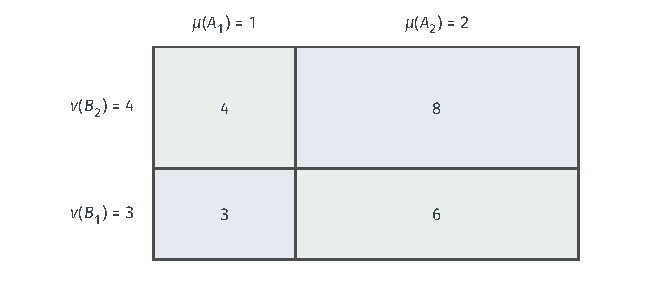
\includegraphics[width=112mm]{figures/01-mathematical-preliminaries-upper/01-mathematical-language-combinatorics-analysis-optimization/tikz/chapter3-concept-processes/product-measure-grid.pdf}
 \caption{列权重为$1,2$，行权重为$3,4$，四个格子的乘积权重为$3,6,4,8$，总量$21$。列宽及行高分别按各自权重成比例，因此面积也按乘积成比例；这些是有限原子空间的权重，不是任意二维分布都必须满足的关系。}
 \label{fig:analysis-process-product-measure-grid}
\end{figure}

\paragraph{欧氏乘积与完备化}

前面分别从欧氏盒和一般矩形构造可测范围，现在核对这两条路线在欧氏空间是否一致。
欧氏空间的Borel范围满足
\begin{equation}
 \mathcal B(\mathbb R^p)\otimes\mathcal B(\mathbb R^q)=\mathcal B(\mathbb R^{p+q}).
 \label{eq:comb-borel-product-structure}
\end{equation}
开盒是低维Borel集合的矩形，给出一个方向的包含。
反过来，坐标投影对低维开盒的原像可写成可数个高维有界开盒的并，因而是Borel集合。
原像保持补集、可数并，这项结论扩展到全部低维Borel集合；
两个投影原像相交便给出Borel矩形，得到另一方向的包含。

把$m_p,m_q$限制在各自Borel范围上，它们的乘积在开盒上给出体积，
由$\sigma$有限唯一扩展，等于Borel范围上的$m_{p+q}$。
再作完备化才得到完备的多维勒贝格测度空间。
即使两个因子测度完备，乘积范围也未必完备，所以应说明采用乘积$\sigma$代数还是其完备化。
函数的累次积分在本节后面讨论，矩形赋值公式还不能单独推出积分换序。


\subsection{区域积分的定义与可积性}
\label{sec:multivariable-riemann-lebesgue}

测度确定区域有多大，被积函数确定各位置贡献多少。现在把一元可测函数与勒贝格积分的定义搬到$\mathbb R^d$上，明确改变的是输入空间，而不是积分的构造方法。

\subsubsection{多元可测函数}

要累计各个函数值对应的区域，首先必须能测量这些区域。与一元情形一样，检查所有阈值以上的原像集合就足够了。
\begin{definition}[多元可测函数]
设$D\in\mathcal L_d$。函数$f:D\to\overline{\mathbb R}$称为勒贝格可测函数，是指对每个$a\in\mathbb R$，集合
\[
 \{\bm x\in D:f(\bm x)>a\}
\]
都属于$\mathcal L_d$。
\end{definition}

连续标量函数的开集原像相对于$D$开，而相对开集可写为$D$与一个欧氏开集的交，因此可测。
连续性仍是可测性的充分条件；例如$\mathbb I_{\mathbb Q^d}$处处不连续，却是可测函数，因为$\mathbb Q^d$可数。
这里没有要求函数输出向量；向量值函数的分量可测性不参与本节区域积分的定义。

\subsubsection{区域积分的定义}

\paragraph{非负标量函数的积分}

先累计非负贡献，就不会遇到正负无穷相消。可测简单函数在每个可测小块上取常值，其积分等于常值乘该块测度再求和；一般非负函数仍由下方的简单函数逼近。
\begin{definition}[非负区域积分]
设$D\in\mathcal L_d$，$f:D\to[0,\infty]$可测。定义
\[
 \int_D f\,\mathrm dm_d
 =\sup_{\substack{0\leq s\leq f\\s\text{为可测简单函数}}}
 \int_D s\,\mathrm dm_d.
\]
若$s=\sum_{j=1}^n c_j\mathbb I_{E_j}$，其中$E_j\subseteq D$可测、两两不交且$c_j\geq0$，则$\int_Ds\,\mathrm dm_d=\sum_jc_jm_d(E_j)$，约定$0\cdot\infty=0$。
\end{definition}

这个积分可以取$+\infty$。在全空间上把$f$作零延拓，就有
$\int_Df\,\mathrm dm_d=\int_{\mathbb R^d}f\mathbb I_D\,\mathrm dm_d$；这里的乘积表示区域外取零。
区域不必是矩形，定义也不要求它的边界零测。

\paragraph{有符号标量函数的积分}

函数可以取正负值时，仍应先分别累计正负贡献。为了得到可以作普通加减的有限积分，本章继续要求绝对值的总贡献有限。
\begin{definition}[区域上的勒贝格可积性]
设$D\in\mathcal L_d$，$f:D\to\overline{\mathbb R}$可测。若
\begin{equation}
 \int_D|f|\,\mathrm dm_d<\infty,
 \label{eq:multivariable-lebesgue-integrability}
\end{equation}
称$f$在$D$上勒贝格可积，并定义
\[
 \int_Df\,\mathrm dm_d=\int_Df^+\,\mathrm dm_d-\int_Df^-\,\mathrm dm_d.
\]
\end{definition}

绝对可积性保证正负部分的积分都有限，也保证$f$几乎处处为有限值。
在零测例外集上把无穷值改成零，不改变积分。若正负部分的积分都为无穷，则不能用两者相减定义勒贝格积分。
例如$\mathbb I_{\mathbb Q^d}$在单位长方体上的积分为零，因为可数集的$d$维测度为零。

\paragraph{二重积分与多重积分}

二维时把上述积分写为
\[
 \iint_Df(x,y)\,\mathrm dx\,\mathrm dy=\int_Df\,\mathrm dm_2;
\]
三维中常记为$\iiint_Df\,\mathrm dV$；$d$维时统一写作
\[
 \int_Df(\bm x)\,\mathrm d\bm x=\int_Df\,\mathrm dm_d.
\]
“二重”或“多重”表示输入维数，并不表示已经选择了逐坐标的计算次序。
例如$f\equiv3$、$D=[0,1]\times[0,2]$时，积分为$3m_2(D)=6$。
函数值在小块上近似常数时，该块贡献近似等于函数值乘面积；这是简单函数累计的几何解释。

\subsubsection{可积性的判别}

\paragraph{有限测度区域上的有界函数}

若$m_d(D)<\infty$，$f$可测且$|f|\leq M<\infty$几乎处处成立，则
\[
 \int_D|f|\,\mathrm dm_d\leq M m_d(D)<\infty.
\]
因此连续函数在紧长方体上可积，更一般地，在任意有限测度区域上有界的可测函数也可积。
无界函数仍可能可积，而无限体积区域上的有界函数未必可积；所检查的始终是绝对值的总累计。

\paragraph{可积控制函数}

若存在非负可积函数$H$使$|f|\leq H$几乎处处成立，则比较不等式给出$\int_D|f|\leq\int_DH<\infty$，从而$f$可积。
这把无界函数的判别转为寻找一个总量有限的上界。后面的非负累次积分还会提供直接计算$\int_D|f|$的方法。

\paragraph{递增区域上的截断}

若$D_n\uparrow D$且各$D_n$可测，单调收敛给出
\[
 \int_D|f|\,\mathrm dm_d
 =\lim_{n\to\infty}\int_{D_n}|f|\,\mathrm dm_d.
\]
因此右侧有有限上界当且仅当$f$可积；可积时，支配收敛又给出$\int_{D_n}f\to\int_Df$。
这样得到的积分值不依赖所选递增覆盖。缺少绝对可积性时，沿某种截断区域得到的正负相消极限，不能替代这里的有限有符号积分。

\subsection{区域积分的基本性质}

多维区域积分仍是测度空间上的勒贝格积分，前面已证明的性质可直接使用。下面固定可测区域$D$，各有符号公式均要求所列函数在相应区域上绝对可积，微元统一写为$\mathrm dm_d$。

\paragraph{加法}

若$f,g$在$D$上可积，则$f+g$也可积，且
\[
 \int_D(f+g)\,\mathrm dm_d=\int_Df\,\mathrm dm_d+\int_Dg\,\mathrm dm_d.
\]
绝对可积性由$|f+g|\leq|f|+|g|$保证，相加公式由一般勒贝格积分的线性给出。

\paragraph{减法}

对同一组可积函数，有
\[
 \int_D(f-g)\,\mathrm dm_d=\int_Df\,\mathrm dm_d-\int_Dg\,\mathrm dm_d.
\]
这里两项都是有限数，因此不会出现无穷减无穷。

\paragraph{常数倍}

若$c\in\mathbb R$且$f$在$D$上可积，则$cf$可积，并满足
\[
 \int_Dcf\,\mathrm dm_d=c\int_Df\,\mathrm dm_d.
\]
系数只改变各位置的标量贡献，不改变积分区域及其测度。

\paragraph{区域可加性}

若$f$在两两不交的可测集合$D_j$之并上可积，则
\[
 \int_{\bigcup_jD_j}f\,\mathrm dm_d=\sum_j\int_{D_j}f\,\mathrm dm_d.
\]
有限并直接来自指示函数的分解，可数并使用一般积分的区域可加性；绝对可积性保证右侧级数绝对收敛。
两块区域允许重叠时，只需扣除被重复计入的交集：
\[
 \int_{A\cup B}f\,\mathrm dm_d
 =\int_Af\,\mathrm dm_d+\int_Bf\,\mathrm dm_d-\int_{A\cap B}f\,\mathrm dm_d.
\]
这由$\mathbb I_{A\cup B}=\mathbb I_A+\mathbb I_B-\mathbb I_{A\cap B}$得到。公共边界零测的有限区域分割，是重叠部分不影响积分的常见情形。

\paragraph{单调性}

若$f\leq g$几乎处处成立，则
\[
 \int_Df\,\mathrm dm_d\leq\int_Dg\,\mathrm dm_d.
\]
特别地，$0\leq f\leq M$且$m_d(D)<\infty$时，有$0\leq\int_Df\leq M m_d(D)$。这也给出忽略一小块区域时的误差上界。

\paragraph{绝对值不等式}

可积函数满足
\[
 \left|\int_Df\,\mathrm dm_d\right|\leq\int_D|f|\,\mathrm dm_d.
\]
它来自$-|f|\leq f\leq|f|$和积分单调性。由于零测集贡献为零，上述所有结论都允许在零测集上修改有限函数值；测度的完备性保证这种修改保持可测。

\subsection{累次积分}
\label{sec:multivariable-iterated-integrals}

直接累计整个区域往往不便计算。固定一个坐标以后，剩下的函数是低一维的截面；先积分这些截面，再累计外层坐标，就得到累次积分。它何时等于区域积分，需要检查非负性或绝对可积性，而不是只交换微分记号。

\subsubsection{截面与累次积分}

对$f:X\times Y\to\overline{\mathbb R}$，固定$x$所得函数$f_x(y)=f(x,y)$称为关于$y$的截面。
若各截面的积分有意义，外层积分也有意义，则
\[
 \int_X\left(\int_Yf(x,y)\,\mathrm d\nu(y)\right)\mathrm d\mu(x)
\]
称为先对$y$、再对$x$的累次积分。反向次序需要另行检查，并不能由这个记号本身推出两者相等。

有限网格上的这种计算就是先求每行加权和，再求行与行之间的加权和；一般乘积测度将同一问题扩展到连续坐标。
乘积测度是一种特定的联合权重构造，一般二元概率分布不必等于两边概率测度的乘积；联合分布与独立性的进一步讨论可参考\BookChapterRef{chap:probability-theory}{卷2《数学准备：概率、因果与决策》的“随机变量与概率基础”章}。

\subsubsection{累次积分的成立条件}

下面固定两个$\sigma$有限测度空间$(X,\mathcal A,\mu)$与$(Y,\mathcal B,\nu)$，先对乘积$\sigma$代数上的可测函数给出结论。
在这个可测范围内，每个截面都可测。若两个因子空间均完备，而函数只对乘积测度的完备化可测，则截面只保证几乎处处可测。若因子尚未完备，应先对因子作完备化，再使用这一表述。

\paragraph{非负可测函数的累次积分}

非负贡献不会因相消而改变总量，因此允许总积分为无穷。Tonelli定理把这一事实精确地表述为两个累次积分与乘积空间积分相等。
\begin{theorem}[Tonelli定理]
\label{thm:analysis-tonelli-fubini}
设$f:X\times Y\to[0,\infty]$对$\mathcal A\otimes\mathcal B$可测。每个截面都可测，两个内层积分函数
\[
 x\longmapsto\int_Yf(x,y)\,\mathrm d\nu(y),\qquad
 y\longmapsto\int_Xf(x,y)\,\mathrm d\mu(x)
\]
也分别可测，且
\[
 \begin{aligned}
 \int_{X\times Y}f\,\mathrm d(\mu\otimes\nu)
 &=\int_X\left(\int_Yf(x,y)\,\mathrm d\nu(y)\right)\mathrm d\mu(x)\\
 &=\int_Y\left(\int_Xf(x,y)\,\mathrm d\mu(x)\right)\mathrm d\nu(y).
 \end{aligned}
\]
三个积分允许共同取$+\infty$。若两个因子空间均完备，函数只对乘积测度的完备化可测，上述等式仍成立，但截面可测性以及内层积分函数的定义都只要求几乎处处成立。
\end{theorem}

\paragraph{绝对可积函数的累次积分}

有符号函数不能只依靠逐行或逐列的有限值来保证换序。先对$|f|$应用非负版本，确认整个乘积空间上的绝对贡献有限，就能排除正负无穷相消。
\begin{theorem}[Fubini定理]
\label{thm:analysis-fubini-integrable}
设$f:X\times Y\to\overline{\mathbb R}$对$\mathcal A\otimes\mathcal B$可测，并满足
$\int_{X\times Y}|f|\,\mathrm d(\mu\otimes\nu)<\infty$。
则$f_x$对几乎每个$x$可积，另一方向的截面也对几乎每个$y$可积。
把内层积分函数在相应例外集上置为零后，它们分别可积，并且
\[
 \begin{aligned}
 \int_{X\times Y}f\,\mathrm d(\mu\otimes\nu)
 &=\int_X\left(\int_Yf(x,y)\,\mathrm d\nu(y)\right)\mathrm d\mu(x)\\
 &=\int_Y\left(\int_Xf(x,y)\,\mathrm d\mu(x)\right)\mathrm d\nu(y).
 \end{aligned}
\]
三个积分都是有限值。若两个因子空间均完备，$f$只对乘积测度的完备化可测，结论仍成立，但截面的可测性和可积性均只作几乎处处的断言。
\end{theorem}

若$f$在零测集上取无穷值，可先将那些值改成零再处理有符号积分。事实上，$N=\{|f|=\infty\}$满足$|f|\geq M\mathbb I_N$对所有$M>0$成立，绝对积分有限强制$N$零测；改值不影响积分。

证明可分为集合与函数两层。对矩形指示函数$\mathbb I_{A\times B}$，三种积分都等于
$\mu(A)\nu(B)$；有限可加性把这个结论扩展到有限分割形成的集合。
从这些集合进入乘积$\sigma$代数中的\emph{任意}可测集合，还需要测度论的扩张论证，
不是仅靠每个矩形上的等式便能完成；完整论证见所引测度论教材
\scite{math-folland1999real}。
本章关注扩张之后的函数层：指示函数的结论经线性组合进入非负简单函数，再经
$s_n\uparrow f$和单调收敛进入任意非负可测函数，得到Tonelli。
若$f$绝对可积，则对$f^+$和$f^-$分别应用Tonelli；绝对积分有限保证两部分不会
出现无穷减无穷，相减才得到Fubini。这里给出证明的依赖路线，不把矩形核对当作
完整证明。


把这两个条件用于$|f|$还有一个实用判别：只要任意一个次序的非负累次积分$\int_X\int_Y|f|$有限，Tonelli就保证区域绝对积分有限，随后才能对$f$使用Fubini。

\subsubsection{累次积分的计算}

设$R=[a,b]\times[c,d]$，其中$a<b$、$c<d$，且$f$在$R$上连续。
此时可以先按一个坐标累计，再按另一个坐标累计，下面三项均为勒贝格积分：
\[
 \begin{aligned}
 \int_R f(x,y)\,\mathrm d(x,y)
 &=\int_a^b\left(\int_c^d f(x,y)\,\mathrm dy\right)\mathrm dx\\
 &=\int_c^d\left(\int_a^b f(x,y)\,\mathrm dx\right)\mathrm dy.
 \end{aligned}
\]
例如$f(x,y)=x+y$在$[0,1]\times[0,2]$上连续，先对$y$积分可得
\[
 \int_0^1\left[xy+\frac{y^2}{2}\right]_{y=0}^{y=2}\,\mathrm dx
 =\int_0^1(2x+2)\,\mathrm dx=3.
\]
内层运算把$x$视为固定数，结果$2x+2$才交给外层积分。这里的$\iint$表示一次区域累计，两个$\int$则表示具体的逐次计算；两者相等须满足上面的条件。

连续函数在紧矩形上绝对可积，前面的Fubini定理保证两种累计次序给出同一结果。

若区域写为$a\leq x\leq b$、$\alpha(x)\leq y\leq\beta(x)$，其中上下边界连续，内积分上下限就应使用$\alpha(x),\beta(x)$。改变积分次序时应重新描述同一个区域。

例如$D=\{(x,y):0\leq y\leq x\leq1\}$上累计$1$，先对$y$积分得到$\int_0^1\int_0^x1\,\mathrm dy\,\mathrm dx=1/2$；反过来，同一区域为$0\leq y\leq1$、$y\leq x\leq1$，故$\int_0^1\int_y^11\,\mathrm dx\,\mathrm dy=1/2$。若只交换微分符号而保留原来的限，就已经改变区域。一般可测函数应先按前面的非负性或绝对可积性条件核验；下面的例子说明缺少这些条件会发生什么。


图~\ref{fig:analysis-process-region-slicing-orders}把刚才的两种累次积分画回同一个三角形区域，突出换序时内层上下限也要改变。
\begin{figure*}[!htbp]
 \centering
 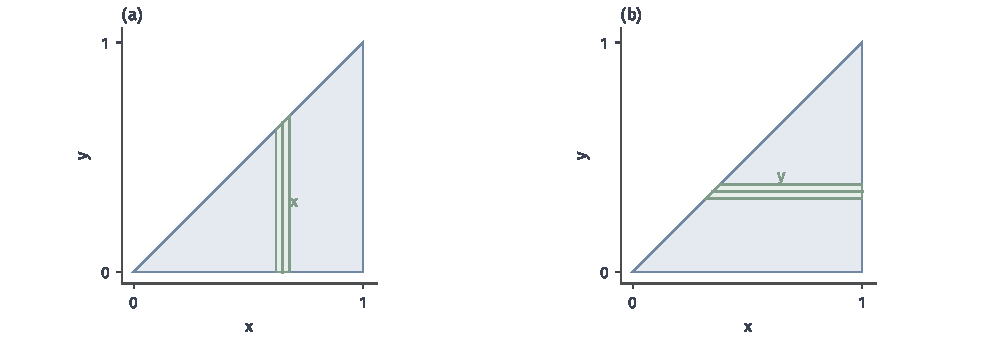
\includegraphics[width=169.0mm]{figures/01-mathematical-preliminaries-upper/01-mathematical-language-combinatorics-analysis-optimization/matplotlib/chapter3-concept-processes/region-slicing-orders.pdf}
 \caption{$D=\{0\leq y\leq x\leq1\}$在两图完全相同。(a) 固定$x$，纵截面为$0\leq y\leq x$；(b) 固定$y$，横截面为$y\leq x\leq1$。绿色窄条仅示意一次切片，图中的条宽不充当实际微元。两种累计$1$都得面积$1/2$；换序依据非负性或绝对可积性，而非图形本身。}
 \label{fig:analysis-process-region-slicing-orders}
\end{figure*}

\subsubsection{积分换序的适用边界}

这里非负性允许无穷值，绝对可积性则排除了依赖积分次序的条件相消。例如在
$\mathbb{N}\times\mathbb{N}$上使用计数测度时，Tonelli说明非负双重级数可以任意交换
求和次序；Fubini说明绝对收敛的双重级数也可以这样做。若既不非负也不绝对可积，
交换次序可能改变结果，甚至一个次序收敛而另一个发散。因此交换积分次序
需要先核对函数的非负性或绝对可积性。

\begin{example}[行列各自可加仍不足以换序]
\label{ex:analysis-iterated-sum-failure}
在正整数索引集$\{1,2,\ldots\}^2$上令
$a_{i,j}=\mathbb I\{j=i\}-\mathbb I\{j=i+1\}$，两边均用计数测度。
每一行只有一个$1$和一个$-1$，故$\sum_j a_{i,j}=0$；
第一列的和为$1$，其余每一列的和为$0$。于是
\[
 \sum_{i=1}^{\infty}\left(\sum_{j=1}^{\infty}a_{i,j}\right)=0,
 \qquad
 \sum_{j=1}^{\infty}\left(\sum_{i=1}^{\infty}a_{i,j}\right)=1.
\]
两种累次和都有有限值，却不相等。每行的绝对值和为$2$，所以整个绝对积分为无穷，
正负部分也各为无穷。失效的是Fubini的绝对可积条件，而非某一行的计算规则。
\end{example}


图~\ref{fig:vol1-add-fubini-cancellation-grid}显示这个例子的两条对角线。逐行的$+1$与$-1$配对，逐列的配对则从第二列才开始；无穷绝对和使这两种配对不能通过Fubini定理互换。
\begin{figure}[!htb]
  \centering
  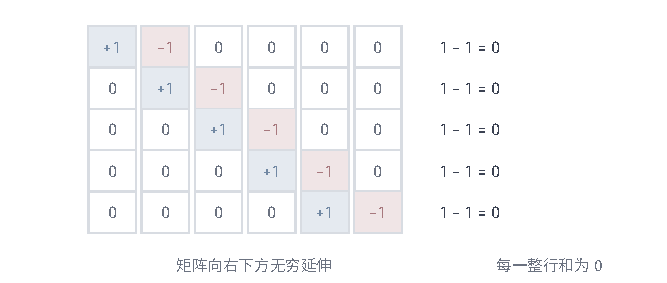
\includegraphics[width=112mm]{figures/01-mathematical-preliminaries-upper/01-mathematical-language-combinatorics-analysis-optimization/tikz/comprehension-additions/fubini-cancellation-grid.pdf}
  \caption{无穷矩阵$a_{i,j}=\mathbb I\{j=i\}-\mathbb I\{j=i+1\}$的左上角，展示前五行、前六列，矩阵向右下方继续。每一整行的和为$0$；第一整列的和为$1$，其他整列的和为$0$。蓝、红单元分别为$+1,-1$，每行绝对和为$2$，因而无穷矩阵不绝对可加。}
  \label{fig:vol1-add-fubini-cancellation-grid}
\end{figure}

$\sigma$有限也有实际作用。在$[0,1]$上让$x$采用Lebesgue测度、$y$采用
定义在所有子集上的计数测度，取非负函数$f(x,y)=\mathbb I\{x=y\}$。
对角线的补集是$[0,1]^2$内的相对开集；由前面欧氏开集的可数有理矩形表示，
它是可数个可测矩形的并。因此取补后，对角线属于乘积$\sigma$代数。
先对$y$计数再对$x$积分得到$1$，
先对$x$求长度再对$y$计数却得到$0$。这里不满足本章Tonelli版本的$\sigma$有限条件，
不能只凭非负性换序。

前面一元积分中的单调收敛、Fatou引理与支配收敛也适用于多维测度空间，因为证明使用简单函数和一般积分性质，并不依赖输入只有一个坐标。

\subsection{区域积分的换元}
\label{sec:multivariable-change-variables}

累次积分保留原坐标，只改变累计次序。换元则用一个向量值映射$T$同时改变位置的坐标表示，因此既要改写标量函数，也要校正每小块的体积。

\subsubsection{换元公式与适用条件}

\paragraph{体积的局部缩放}

一元换元用导数把参数增量换成长度增量；多元换元要把参数小块换成体积。
对方阵$\bm A$，$|\det\bm A|$是其线性映射对体积的放大倍数。
二维中，两列向量张成的平行四边形面积为$|\det\bm A|$；对角缩放$\operatorname{diag}(a_1,\ldots,a_d)$的比例为$\prod_j|a_j|$。
绝对值使方向反转后普通体积仍非负。

若$T$可微，Jacobian矩阵$\bm J_T(\bm x)$给出一点附近的线性近似，因此局部体积权重应是$|\det\bm J_T(\bm x)|$。
这个局部说明还不是整个积分公式的证明：整体上还必须控制近似误差，并确保参数化不会在正体积区域重复覆盖。

\paragraph{勒贝格积分的换元}

使用开集之间的$C^1$微分同胚，可以同时保证局部体积规则和全局单次覆盖。下面直接给出勒贝格版本，连续被积函数只是其中的一个特例。
\begin{theorem}[区域积分的换元公式]
设$U,V\subseteq\mathbb R^d$为开集，$T:U\to V$为$C^1$双射，逆映射也为$C^1$，且$\det\bm J_T$处处非零。
对任意非负勒贝格可测函数$g:V\to[0,\infty]$，有
\begin{equation}
 \int_Vg(\bm y)\,\mathrm d\bm y
 =\int_Ug(T(\bm x))|\det\bm J_T(\bm x)|\,\mathrm d\bm x,
 \label{eq:measurable-change-variables}
\end{equation}
允许共同值为$+\infty$。若$g$有符号且在$V$上绝对可积，则变换后的函数也绝对可积，等式仍成立并取有限值。
\end{theorem}

这类变换及其逆在局部紧邻域上是Lipschitz映射，因而保持零测集为零测集；结合Borel可测性，才能处理勒贝格完备化增加的集合。
一般定理先建立可测集合的体积变换，再从指示函数进入简单函数，最后以单调逼近得到非负函数的公式；有符号情形对$|g|$、$g^+$和$g^-$分别应用非负结论即可。
这里说明证明的依赖关系，集合层的体积变换定理引用测度论教材\scite{math-folland1999real}，不把逐点线性化当作完整证明。

若只在可测子区域$D\subseteq U$上积分，对$V$中的函数$g\mathbb I_{T(D)}$应用同一公式，即得
\begin{equation}
 \int_{T(D)}g(\bm y)\,\mathrm d\bm y
 =\int_Dg(T(\bm x))|\det\bm J_T(\bm x)|\,\mathrm d\bm x.
 \label{eq:analysis-multivariate-change-variables}
\end{equation}
这里不另加有界或边界零测的要求；所需条件仍是非负可测，或者有符号且绝对可积。
若参数化只在去掉零测边界或接缝以后为微分同胚，可以先在该范围内换元，再补回零测集。
若在正测度区域重复覆盖，则不能直接使用这个单次覆盖版本。

\subsubsection{常用坐标变换}

\paragraph{极坐标}

圆盘的边界用直角坐标描述时，积分上下限会含平方根。以半径和角度作为坐标，区域变成参数矩形，但面积权重必须增加半径因子。
\begin{example}[极坐标中的面积权重]
\label{ex:analysis-polar-coordinate-jacobian}
令$D=\{\bm{x}\in\mathbb{R}^2:\lVert\bm{x}\rVert_2\leq1\}$，并令
$T(r,\theta)=(r\cos\theta,r\sin\theta)$。在开集
$(0,1)\times(0,2\pi)$上，$T$是到开圆盘内部去掉原点和正$x$轴径向接缝后的区域的
连续可微双射，逆映射也连续可微。其Jacobian矩阵的行列式为
\[   \det
\begin{bmatrix}     \cos\theta & -r\sin\theta\\     \sin\theta & r\cos\theta
\end{bmatrix}   =r. \]
为了避开原点和接缝，可先限制$\varepsilon\leq r\leq1-\varepsilon$、$\varepsilon\leq\theta\leq2\pi-\varepsilon$，在每个这样的闭矩形上使用换元公式。遗漏的中心小圆盘、外侧窄环与接缝窄扇形面积随$\varepsilon\downarrow0$趋零；对有界被积函数，它们的累计贡献也趋零。因此取极限得到
\[   \int_D1\,\mathrm{d}\bm{x}   =   \int_0^{2\pi}\int_0^1r\,\mathrm{d}r\,\mathrm{d}\theta   =\pi. \]
这里积分上下限包含端点不改变积分值。若参数化在一片有正面积或体积的区域上重复覆盖，则不能直接使用
上述双射版本，否则同一点会被重复计数。
\end{example}

图~\ref{fig:vol1-add-polar-area-weight}说明半径因子来自哪里。同样的角度变化在较大半径处扫过更长的弧，故同样大小的参数块对应更大的面积，积分权重必须随半径变化。
\begin{figure}[!htb]
  \centering
  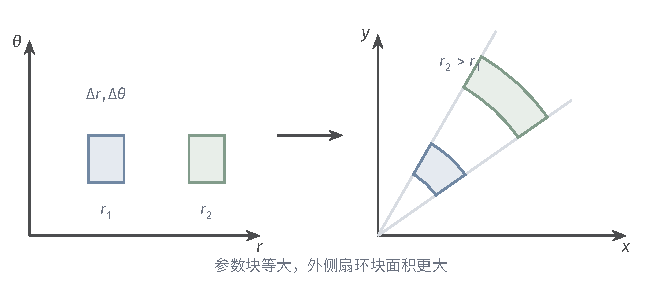
\includegraphics[width=112mm]{figures/01-mathematical-preliminaries-upper/01-mathematical-language-combinatorics-analysis-optimization/tikz/comprehension-additions/polar-area-weight.pdf}
  \caption{极坐标映射中的两个等大参数块，具有相同的$\Delta r,\Delta\theta$，但外侧半径$r_2$较大。对应扇环块的精确面积为$(r\Delta r+(\Delta r)^2/2)\Delta\theta$，一阶项为$r\Delta r\Delta\theta$，因此面积元为$r\,\mathrm dr\,\mathrm d\theta$。图只比较局部块，坐标原点与接缝的处理见正文。}
  \label{fig:vol1-add-polar-area-weight}
\end{figure}



\paragraph{柱坐标}

在三维中，柱坐标变换为$(x,y,z)=(r\cos\theta,r\sin\theta,z)$，体积元是$r\,\mathrm dr\,\mathrm d\theta\,\mathrm dz$。
例如半径$R$、高度$H$的圆柱体体积为
\[
 \int_0^H\int_0^{2\pi}\int_0^R r\,\mathrm dr\,\mathrm d\theta\,\mathrm dz=\pi R^2H.
\]
\paragraph{球坐标}

球坐标用到原点的距离$\rho$、从正$z$轴量起的夹角$\varphi$和绕$z$轴的角$\theta$：
\[
 (x,y,z)=(\rho\sin\varphi\cos\theta,\rho\sin\varphi\sin\theta,\rho\cos\varphi).
\]
其Jacobian行列式的绝对值为$\rho^2\sin\varphi$，故体积元为$\rho^2\sin\varphi\,\mathrm d\rho\,\mathrm d\varphi\,\mathrm d\theta$。
半径$R$的球由$0\leq\rho\leq R$、$0\leq\varphi\leq\pi$、$0\leq\theta\leq2\pi$描述，体积为
\[
 \int_0^{2\pi}\int_0^\pi\int_0^R\rho^2\sin\varphi\,\mathrm d\rho\,\mathrm d\varphi\,\mathrm d\theta
 =\frac{4\pi R^3}{3}.
\]
这里和极坐标一样，在内部单次覆盖处使用换元公式；坐标轴、原点及接缝的零测遗漏用极限补回。

\subsection{参数积分}
\label{sec:multivariable-parameter-integrals}

前面改变的是空间坐标。现在固定积分区域，让标量函数依赖一个实参数$\theta$，研究积分所得的数如何随这个参数变化；这分别涉及连续性、求导和端点变化三个问题。

\subsubsection{参数积分的定义}

设$(X,\mathcal A,\mu)$为测度空间，$I$为实参数区间，且对每个$\theta\in I$，$g(\cdot,\theta)$都是可积的标量函数。定义
\[
 G(\theta)=\int_Xg(x,\theta)\,\mathrm d\mu(x).
\]
固定参数后，$x$是被积变量；积分完成以后，$G$是一元参数函数。点态连续或点态可微只描述每个$x$处的变化，要将它们传递给$G$，还要控制整族函数的总贡献。

\subsubsection{参数积分的连续性}

参数趋近时，积分贡献可能集中到越来越小的区域，或移向无穷远。用同一个可积函数控制附近全部参数的贡献，可以通过支配收敛排除这些情况。
\begin{theorem}[可积控制下参数积分的连续性]
设$\theta_0\in I$，每个$g(\cdot,\theta)$可测。假设存在$\theta_0$在$I$中的一个相对邻域$J$、同一个可测零测集$N$及非负可积函数$h$，使对每个$x\notin N$，$g(x,\cdot)$在$\theta_0$连续，且
$|g(x,\theta)|\leq h(x)$对所有$\theta\in J$成立。
则$G(\theta)$在$J$上有有限值，并在$\theta_0$连续。
\end{theorem}
\begin{proof}
任取$\theta_n\to\theta_0$，充分大时$\theta_n\in J$。在$X\setminus N$上，$g(x,\theta_n)\to g(x,\theta_0)$，且绝对值都不超过$h(x)$。
支配收敛给出$G(\theta_n)\to G(\theta_0)$，由序列判据得到连续性。
\end{proof}

例如$g(x,\theta)=e^{-\theta x}$在$[0,\infty)$上积分，$\theta>0$时$G(\theta)=1/\theta$。
固定$\theta_0>0$，在其邻域内可由$e^{-\theta_0x/2}$支配，故$G$在$\theta_0$连续。控制函数只需覆盖所考察参数点的邻域，不要求同一上界适用于全部参数。

\subsubsection{积分号下求导}

积分号下求导实际要交换参数差商的极限与积分。各点偏导数存在只确定差商的点态极限；同一个可积函数控制全部差商，才足以将这个极限移入积分号。
\begin{theorem}[可积导数界下的积分号内求导]
固定$\theta_0$，设对每个$\theta\in I$，
$x\mapsto g(x,\theta)$可测，其中$I$是包含$\theta_0$的开区间，并且
$g(\cdot,\theta_0)$可积。假设存在一个可测零测集$N$，使每个$x\notin N$处的
$\theta\mapsto g(x,\theta)$在整个$I$内可微；对每个$\theta$，
偏导数作为$x$的函数可测，并且存在非负可积函数$h$使
\begin{equation}
  \left|
    \frac{\partial g}{\partial\theta}(x,\theta)
  \right|
  \leq h(x)
  \quad
  \text{对所有$x\notin N$及所有$\theta\in I$成立},
\label{eq:analysis-parameter-derivative-domination}
\end{equation}

则$I$内每个参数截面都可积，且
\begin{equation}
  G'(\theta_0)
  =
  \int_X
  \frac{\partial g}{\partial\theta}(x,\theta_0)
  \,\mathrm{d}\mu(x).
\label{eq:analysis-differentiate-under-integral}
\end{equation}
\end{theorem}
\begin{proof}
中值定理先给出
$|g(x,\theta)-g(x,\theta_0)|\leq|\theta-\theta_0|h(x)$，
所以$I$中每个$g(\cdot,\theta)$都可积，$G$在邻域内有有限值。
对非零$t$且$\theta_0+t\in I$，令
\[
 q_t(x)=\frac{g(x,\theta_0+t)-g(x,\theta_0)}{t}.
\]
中值定理又给出
\[
 |q_t(x)|\leq h(x)\qquad(x\notin N).
\]
差商在那里趋于$\partial g/\partial\theta(x,\theta_0)$。
对任意非零序列$t_n\to0$应用支配收敛，得到同一个积分极限；
由实数极限的序列判据，这就是$t\to0$的双侧极限。这正是所述导数公式。
\end{proof}

这里的零测集$N$和控制函数$h$都不能随参数改变。参数范围不可数，不能靠取全部参数例外集的并自动获得一个零测集。
条件~\eqref{eq:analysis-parameter-derivative-domination}是一组便于核对的充分条件；也可在更一般的版本中直接控制参数差商。

例如令$g(x,\theta)=e^{-\theta x}$，$x\in[0,\infty)$、$\theta>0$，
并用Lebesgue测度积分。固定$\theta_0>0$后取
$I=(\theta_0/2,3\theta_0/2)$，则
$|\partial_\theta g|=xe^{-\theta x}\leq xe^{-\theta_0x/2}=:h(x)$。
分部积分给出$\int_0^\infty h(x)\,\mathrm dx=4/\theta_0^2<\infty$，
没有需要删除的例外点，故
$G'(\theta_0)=-\int_0^\infty xe^{-\theta_0x}\,\mathrm dx=-1/\theta_0^2$，
与$G(\theta)=1/\theta$的直接求导一致。
若把参数范围放大到任意接近零的正数，便不能沿用这个固定的控制函数；
交换结论所需的是所考察参数点附近的统一控制。

\begin{example}[参数积分中的控制函数失效]
\label{ex:analysis-parameter-integral-failure}
下面考察参数域边界处对应的右求导问题。对$\theta\geq0$与$x\in(0,1)$，定义
\[   g(x,\theta)   =
\begin{cases}     \dfrac{\theta x}{x^2+\theta^2}, & \theta>0,\\[5pt]     0, & \theta=0.
\end{cases} \]
在$\theta=0$处，对每个固定$x>0$，关于$\theta$的右偏导数都等于$1/x$，但$1/x$在$(0,1)$上不可积。
直接积分得到
\[   G(\theta)   =   \frac{\theta}{2}   \log\left(\frac{1+\theta^2}{\theta^2}\right)   \quad(\theta>0),   \qquad G(0)=0. \]
于是$G(\theta)/\theta$在$\theta\downarrow0$时发散，$G$在$0$处没有有限右导数。积分内的
逐点右导数虽然存在，却缺少统一可积控制；因此这里不能交换右求导与积分。
\end{example}

\subsubsection{变限积分的求导}

前面的差商固定了积分区域。如果端点也变化，即使被积函数不依赖参数，积分仍然会变化。例如$G(\theta)=\int_0^\theta1\,\mathrm dx=\theta$的导数为一，只计算被积函数的参数偏导会遗漏这一贡献。
连续性能够逐点确定端点处的函数值，并将区间长度的变化转为边界贡献。
\begin{theorem}[变限参数积分的求导]
设$a(\theta),b(\theta)$在$\theta_0$附近可微，且$a(\theta)<b(\theta)$。
若$g(x,\theta)$和$\partial_\theta g(x,\theta)$在包含这些邻近积分区间的一个紧矩形上连续，则
\begin{equation}
 \begin{aligned}
 \frac{\mathrm d}{\mathrm d\theta}\int_{a(\theta)}^{b(\theta)}g(x,\theta)\,\mathrm dx
 &=\int_{a(\theta)}^{b(\theta)}\partial_\theta g(x,\theta)\,\mathrm dx\\
 &\quad+g(b(\theta),\theta)b'(\theta)
 -g(a(\theta),\theta)a'(\theta).
 \end{aligned}
\label{eq:measurable-moving-boundary-integral}
\end{equation}
\end{theorem}
\begin{proof}
记$a_0=a(\theta_0)$、$b_0=b(\theta_0)$。积分差可分解为
\[
 \begin{aligned}
 G(\theta)-G(\theta_0)
 &=\int_{a_0}^{b_0}\bigl[g(x,\theta)-g(x,\theta_0)\bigr]\,\mathrm dx\\
 &\quad+\int_{b_0}^{b(\theta)}g(x,\theta)\,\mathrm dx
 -\int_{a_0}^{a(\theta)}g(x,\theta)\,\mathrm dx.
 \end{aligned}
\]
短区间积分按端点次序采用有向约定。第一项除以$\theta-\theta_0$后，由固定区间内的积分号下求导趋于$\int_{a_0}^{b_0}\partial_\theta g(x,\theta_0)\,\mathrm dx$。
连续性使第二项等于
$g(b_0,\theta_0)[b(\theta)-b_0]+o(|b(\theta)-b_0|)$。端点的可微性保证$|b(\theta)-b_0|=O(|\theta-\theta_0|)$，所以它的差商趋于$g(b_0,\theta_0)b'(\theta_0)$。
第三项同理，并保留前面的负号，得到下端点贡献。三项相加即得公式。
\end{proof}

采用紧矩形上的连续性，是一组便于核对的充分条件。对一般可测函数，端点值还需有相应的取值与极限意义，不能仅凭几乎处处等价类任意指定边界读数。

\FloatBarrier

\par\Needspace{10\baselineskip}
\section{路径积分}
\label{sec:multivariable-path-integration}

细线的质量由线密度和长度决定，力沿路线做功还取决于位移方向。
两种问题的积分位置都是一条路径，但被积对象不同：线密度是标量函数，力是向量场。
第一类路径积分用弧长累计标量值，第二类路径积分先取向量场与有向位移的内积，再累计这个标量。
两者都要先规定路径的参数化；下面分别说明各自的定义、可积要求、性质和计算方法，最后研究第二类路径积分何时只依赖端点。所有参数积分均为勒贝格积分\scite{math-openstax-calculus3}。

\subsection{参数路径与弧长}
\label{sec:multivariable-line-integrals}

路径既要说明走过哪些位置，也要说明行进次序。弧长则把参数增量换成实际路程，为第一类路径积分提供权重。

\subsubsection{路径的定义}

\paragraph{参数化路径}

同一个几何点集可以按不同速度、不同方向走过，甚至被重复走过。用区间到空间的连续映射，可以把这些行进信息一并保留下来。
\begin{definition}[路径]
设$a<b$。连续映射$\gamma:[a,b]\to\mathbb R^d$称为一条\term{路径}（path），$\gamma(a)$和$\gamma(b)$分别为起点和终点；若两者相等，称为闭路径。
集合$C=\gamma([a,b])$称为路径的像。
\end{definition}

参数$t$指定行进次序，像集$C$只记录经过的位置。例如$\gamma(t)=(t,t)^\top$、$0\leq t\leq1$从$(0,0)$走到$(1,1)$；$\eta(u)=(u/2,u/2)^\top$、$0\leq u\leq2$沿同一方向走过同一条线段。
二者的速度不同，但没有改变行进次数。相反，沿同一线段往返的路径不能只凭这个线段的像集确定累计量。

\paragraph{分段光滑路径}

折线在转角处没有唯一切线，但每一条线段仍可计算速度。为了把这些路径也纳入计算，允许在有限个参数点处分段。
\begin{definition}[分段光滑路径]
若存在分割$a=t_0<t_1<\cdots<t_n=b$，使$\gamma$在每个$[t_{j-1},t_j]$上为$C^1$映射，称$\gamma$为分段$C^1$路径，也称分段光滑路径。
若每段内部还满足$\gamma'(t)\neq\bm0$，称该路径分段正则。
\end{definition}

这里每一段的导数都连续延拓到该段端点，相邻两段的端点导数不必相同。
本节路径积分均在分段$C^1$路径上定义，折点处的有限个取值不影响参数积分；单位切向量只在速度非零处使用。

\subsubsection{路径的长度}

\paragraph{弧长}

用路径上依次选出的点连接成折线，可以从下方估计实际路程。细分后取所有这类折线长度的上确界，就得到不依赖所选分割的长度。
\begin{definition}[路径的弧长]
路径$\gamma:[a,b]\to\mathbb R^d$的弧长定义为
\[
 \ell(\gamma)=\sup_{a=t_0<\cdots<t_n=b}
 \sum_{j=1}^n\lVert\gamma(t_j)-\gamma(t_{j-1})\rVert_2.
\]
上确界取遍$[a,b]$的全部有限分割；若此值有限，称路径可求长。
\end{definition}

对光滑路径，小段位移由速度乘参数增量近似。因此弧长可以由速度的大小累计，得到下面的计算公式。
\begin{theorem}[分段光滑路径的弧长]
若$\gamma:[a,b]\to\mathbb R^d$分段$C^1$，则它可求长，且
\[
 \ell(\gamma)=\int_a^b\lVert\gamma'(t)\rVert_2\,\mathrm dt.
\]
\end{theorem}
\begin{proof}
先在一段$C^1$区间上证明。由各坐标的一元基本定理，
$\gamma(v)-\gamma(u)=\int_u^v\gamma'(t)\,\mathrm dt$，这里向量积分表示对各分量分别积分。将此等式与弦方向的单位向量取内积，再用Cauchy--Schwarz不等式，可知每段弦长不超过$\int_u^v\lVert\gamma'(t)\rVert_2\,\mathrm dt$。弦为零时这个不等式直接成立。相加后，任意内接折线的长度都不超过速度范数的积分。

反过来，$\gamma'$在紧区间上一致连续。若分割足够细，使每个小区间上$\gamma'$的振幅小于$\varepsilon$，并在其中取一点$\xi_j$，则弦向量与$\gamma'(\xi_j)(t_j-t_{j-1})$的距离不超过$\varepsilon(t_j-t_{j-1})$。
同一小区间上$\lVert\gamma'\rVert_2$的积分与$\lVert\gamma'(\xi_j)\rVert_2(t_j-t_{j-1})$的差也不超过这个数。
因此速度积分与该折线长度的差不超过$2\varepsilon(b-a)$。令$\varepsilon\downarrow0$，得到反向不等式。分段$C^1$的情形对各段相加即可。
\end{proof}

记$s(t)=\int_a^t\lVert\gamma'(u)\rVert_2\,\mathrm du$为截至参数$t$的累计路程，常将长度权重写为
$\mathrm ds=\lVert\gamma'(t)\rVert_2\,\mathrm dt$。例如前述对角线段的速度为$(1,1)^\top$，长度为$\sqrt2$；两个坐标分别变化$1$，并不意味着实际长度为$2$。

\subsection{第一类路径积分}

第一类路径积分的被积对象是沿路径给定的标量函数，例如线密度。每一小段的贡献是函数值乘实际弧长，因此不需要指定力或其他向量场。

\subsubsection{定义与可积性}

\paragraph{按弧长的积分}

把路径分成小段并累计函数值乘小段长度，会得到弧长权重$\lVert\gamma'(t)\rVert_2$。用这个权重定义积分，也允许处理沿路径可测而不连续的标量函数。
\begin{definition}[第一类路径积分]
设$\gamma:[a,b]\to\mathbb R^d$分段$C^1$，$h:C\to\mathbb R$，其中$C=\gamma([a,b])$，且$h\circ\gamma$在参数区间上勒贝格可测。
若$h\geq0$，定义\term{第一类路径积分}（scalar line integral）为
\begin{equation}
 \int_\gamma h\,\mathrm ds
 =\int_a^b h(\gamma(t))\lVert\gamma'(t)\rVert_2\,\mathrm dt,
 \label{eq:analysis-scalar-line-integral}
\end{equation}
允许取$+\infty$。对一般有符号$h$，本节称它沿$\gamma$可积，是指
\[
 \int_a^b |h(\gamma(t))|\lVert\gamma'(t)\rVert_2\,\mathrm dt<\infty;
\]
此时由正负部分之差定义积分，式~\eqref{eq:analysis-scalar-line-integral}仍成立并取有限值。
\end{definition}

$h=1$给出弧长；非负线密度的积分给出细线质量。若$h$在紧像集$C$上连续，它有界，因而绝对积分不超过$\sup_C|h|\,\ell(\gamma)<\infty$。连续性是方便的充分条件，并非定义本身的要求。

这里必须知道路径上的实际取值，以及它与参数复合后的可测性。仅有环境区域中的勒贝格可积性不能替代这个要求。
例如$h(x,y)=\mathbb I\{y=0\}$在平面几乎处处为零，但沿$\gamma(t)=(t,0)$、$0\leq t\leq1$的弧长积分为$1$。
面积零测集仍可有正长度，不能从平面函数的几乎处处等价类直接读出线积分。

\subsubsection{积分的基本性质}

下面的有符号公式都假设相应标量函数沿所讨论路径可积。将参数公式代入一元勒贝格积分的性质，就能逐项得到这些结论。

\paragraph{加法}

若$h,k$沿$\gamma$可积，则$h+k$也沿$\gamma$可积，且
\[
 \int_\gamma(h+k)\,\mathrm ds=\int_\gamma h\,\mathrm ds+\int_\gamma k\,\mathrm ds.
\]
绝对可积性由$|h+k|\leq|h|+|k|$保证。

\paragraph{减法}

对同一组可积函数，将$k$换成其相反函数，得到
\[
 \int_\gamma(h-k)\,\mathrm ds=\int_\gamma h\,\mathrm ds-\int_\gamma k\,\mathrm ds.
\]
两边均为有限数，不涉及无穷相消。

\paragraph{常数倍}

若$c\in\mathbb R$且$h$沿$\gamma$可积，则
\[
 \int_\gamma ch\,\mathrm ds=c\int_\gamma h\,\mathrm ds.
\]
这表示将每一小段上的密度同时放大$c$倍，累计量也按相同比例变化。

\paragraph{路径拼接}

若$\gamma_1$的终点是$\gamma_2$的起点，记依次走过两条路径的拼接为$\gamma_1*\gamma_2$。沿两条路径分别可积时，
\[
 \int_{\gamma_1*\gamma_2}h\,\mathrm ds
 =\int_{\gamma_1}h\,\mathrm ds+\int_{\gamma_2}h\,\mathrm ds.
\]
参数区间的可加性给出这个等式；若某段被重复走过，它的贡献也会重复计入。

\paragraph{重参数化与方向无关}

设$t=\eta(u)$是两个参数区间之间单调、端点相配的分段$C^1$微分同胚。链式法则给出
$\lVert(\gamma\circ\eta)'(u)\rVert_2=\lVert\gamma'(\eta(u))\rVert_2|\eta'(u)|$，再用一元换元可得
\[
 \int_{\gamma\circ\eta}h\,\mathrm ds=\int_\gamma h\,\mathrm ds.
\]
无论$\eta$递增还是递减，绝对值都保留非负弧长权重，因此反向行进不改变第一类积分。这个结论只改变行进速度或方向，不改变行进次数。

\paragraph{单调性}

若$h\leq k$在路径上成立，则非负弧长权重保证
\[
 \int_\gamma h\,\mathrm ds\leq\int_\gamma k\,\mathrm ds.
\]
这里比较的是同一路径上的两个标量函数。

\paragraph{绝对值不等式}

由一元积分的绝对值不等式可得
\[
 \left|\int_\gamma h\,\mathrm ds\right|
 \leq\int_\gamma|h|\,\mathrm ds
 \leq\sup_C|h|\,\ell(\gamma).
\]
最后一个不等式在$h$有界时适用。它用路径长度和函数的大小控制累计量。

\subsubsection{积分的计算}

计算时先参数化路径，再将标量函数乘速度范数，转为一元积分；折点两侧逐段相加。
例如在线段$\gamma(t)=(t,t)^\top$、$0\leq t\leq1$上取$h(x,y)=x+y$，得到
\[
 \int_\gamma h\,\mathrm ds=\int_0^1 2t\sqrt2\,\mathrm dt=\sqrt2.
\]
累计的是沿线的函数值，而非线段下方的平面面积。

沿$x$递增的图像路径$\gamma(x)=(x,\psi(x))^\top$，$a\leq x\leq b$，若$\psi$为$C^1$，则
\[
 \int_\gamma h\,\mathrm ds
 =\int_a^b h(x,\psi(x))\sqrt{1+\psi'(x)^2}\,\mathrm dx.
\]
根号是图像路径的速度范数，不能省略为单独的$\mathrm dx$权重。

\subsection{第二类路径积分}

做功问题中，被积对象变成向量场：每个位置给出一个向量。位移方向改变时，向量在该方向上的分量可能变号，因此需要有向累计。

\subsubsection{定义与可积性}

\paragraph{向量场}

要在空间中描述力，必须为每个位置同时给出大小和方向。定义域与输出空间具有相同维数的向量值映射，正适合记录这种信息。
\begin{definition}[向量场]
设$U\subseteq\mathbb R^d$。映射$\bm F:U\to\mathbb R^d$称为$U$上的\term{向量场}（vector field）。
\end{definition}

向量场的输入是位置，输出是该位置的一个向量。例如$\bm F(x,y)=(-y,x)^\top$给出的向量与以原点为圆心的圆相切。
若它表示力，小段做功是场值与位移的内积，只有沿位移方向的分量参与做功。

\paragraph{有向线积分}

沿参数路径的小段有向位移近似为$\gamma'(t)\,\mathrm dt$。将场值与这个位移取内积，得到一个可以在参数区间上累计的标量函数。
\begin{definition}[第二类路径积分]
设$\gamma:[a,b]\to U$分段$C^1$，$\bm F:U\to\mathbb R^d$为向量场。
若$\bm F\circ\gamma$的每个分量勒贝格可测，且$t\mapsto\bm F(\gamma(t))^\top\gamma'(t)$绝对可积，定义\term{第二类路径积分}（vector line integral）为
\begin{equation}
 \int_\gamma\bm F\mathbin{\cdot}\mathrm d\bm r
 =\int_a^b\bm F(\gamma(t))^\top\gamma'(t)\,\mathrm dt.
 \label{eq:analysis-vector-line-integral}
\end{equation}
\end{definition}

在平面中，$\bm F=(P,Q)^\top$时写为$\int_\gamma P\,\mathrm dx+Q\,\mathrm dy$；三维中再加$R\,\mathrm dz$。
若$\bm F$在路径像集上连续，复合函数在各段连续，从而上述参数积分绝对可积。
更一般地，可测性以及$\int_a^b\lVert\bm F(\gamma(t))\rVert_2\lVert\gamma'(t)\rVert_2\,\mathrm dt<\infty$也是充分条件，因为内积的绝对值不超过范数之积。

速度非零处的单位切向量为$\bm\tau=\gamma'/\lVert\gamma'\rVert_2$，所以
$\bm F\cdot\mathrm d\bm r=(\bm F^\top\bm\tau)\,\mathrm ds$。
第二类积分累计的是向量场的切向分量；沿闭路径累计时也称\term{环流}（circulation）。它可以转写为一个标量的弧长积分，但这个标量随所选行进方向改变。


图~\ref{fig:analysis-process-line-density-work}用同一条线段对照弧长累计与有向位移累计，避免把速度范数和内积混用。
\begin{figure}[!htbp]
 \centering
 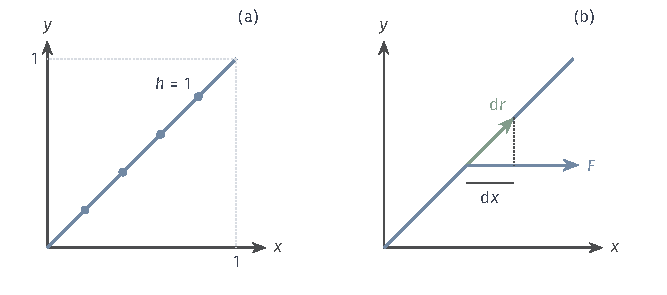
\includegraphics[width=112mm]{figures/01-mathematical-preliminaries-upper/01-mathematical-language-combinatorics-analysis-optimization/tikz/chapter3-concept-processes/line-density-work.pdf}
 \caption{路径均为$\gamma(t)=(t,t)^\top$，$0\leq t\leq1$。(a) 常数线密度$h=1$按弧长累计，得到$\sqrt2$。(b) 常向量场$F=(1,0)^\top$只取位移的水平分量，做功为$1$；图中$\mathrm dx$是$\mathrm dr$的水平投影。相同路径、不同被积对象和权重给出不同积分。}
 \label{fig:analysis-process-line-density-work}
\end{figure}

\subsubsection{积分的基本性质}

下列公式均由内积和一元勒贝格积分的相应性质得到，并要求涉及的有向积分存在且有限。

\paragraph{加法}

若$\bm F$和$\bm G$沿$\gamma$可积，则
\[
 \int_\gamma(\bm F+\bm G)\cdot\mathrm d\bm r
 =\int_\gamma\bm F\cdot\mathrm d\bm r+\int_\gamma\bm G\cdot\mathrm d\bm r.
\]
这里相加的是两个向量场，内积后才得到被积标量。

\paragraph{减法}

将$\bm G$换成其相反场，得到
\[
 \int_\gamma(\bm F-\bm G)\cdot\mathrm d\bm r
 =\int_\gamma\bm F\cdot\mathrm d\bm r-\int_\gamma\bm G\cdot\mathrm d\bm r.
\]
可积性使两个方向的累计量都有限，因而可以相减。

\paragraph{常数倍}

对实数$c$，有
\[
 \int_\gamma c\bm F\cdot\mathrm d\bm r
 =c\int_\gamma\bm F\cdot\mathrm d\bm r.
\]
系数只改变场的大小和符号，不改变路径的几何形状与方向。

\paragraph{路径拼接}

若$\gamma_1$和$\gamma_2$首尾相接，则
\[
 \int_{\gamma_1*\gamma_2}\bm F\cdot\mathrm d\bm r
 =\int_{\gamma_1}\bm F\cdot\mathrm d\bm r
 +\int_{\gamma_2}\bm F\cdot\mathrm d\bm r.
\]
这使分段光滑路径可以逐段计算；每段都必须保留该次行进的方向。

\paragraph{方向反转}

记反向路径为$\gamma^{-}(u)=\gamma(a+b-u)$，$a\leq u\leq b$。它的速度是原速度的相反向量，一元换元因此给出
\[
 \int_{\gamma^{-}}\bm F\cdot\mathrm d\bm r
 =-\int_\gamma\bm F\cdot\mathrm d\bm r.
\]
这与第一类积分反向后不变相区别：长度始终非负，有向位移则改变符号。

\paragraph{重参数化}

若$t=\eta(u)$为端点相配、严格递增的分段$C^1$微分同胚，则
$(\gamma\circ\eta)'(u)=\gamma'(\eta(u))\eta'(u)$。在参数公式中应用换元，得到
\[
 \int_{\gamma\circ\eta}\bm F\cdot\mathrm d\bm r
 =\int_\gamma\bm F\cdot\mathrm d\bm r.
\]
严格递减的重参数化会反转方向，因而积分变号。方向相同的不同速度不会改变积分，重复行进的次数却仍会被保留。

\paragraph{绝对值不等式}

由积分的三角不等式和内积的Cauchy--Schwarz不等式可得
\[
 \left|\int_\gamma\bm F\cdot\mathrm d\bm r\right|
 \leq\int_\gamma\lVert\bm F\rVert_2\,\mathrm ds.
\]
右侧有限时，它为做功或环流的绝对值提供上界；若右侧为$+\infty$，不等式仍成立，但不能用来证明左侧有限。

\subsubsection{积分的计算}

参数化以后，第二类积分把场值与速度取内积，不乘速度范数。例如常向量场$\bm F=(1,0)^\top$沿前述对角线段的积分为
\[
 \int_0^1(1,0)\cdot(1,1)\,\mathrm dt=1.
\]
同一路径的长度为$\sqrt2$，两种结果对应不同的被积对象和局部权重。

对平面图像路径$\gamma(x)=(x,\psi(x))^\top$、$a\leq x\leq b$，$\bm F=(P,Q)^\top$时有
\[
 \int_\gamma\bm F\cdot\mathrm d\bm r
 =\int_a^b\bigl[P(x,\psi(x))+Q(x,\psi(x))\psi'(x)\bigr]\,\mathrm dx.
\]
下面固定起终点比较不同路径，观察这个积分是否还会依赖路线。

\begin{example}[半圆和直径]
\label{ex:analysis-path-integral-comparison}
取$\gamma(t)=(\cos t,\sin t)$，$0\leq t\leq\pi$。它从$(1,0)$沿上半圆走到$(-1,0)$，速度范数为$1$，故$\int_\gamma1\,\mathrm ds=\pi$。
对常场$(1,0)^\top$，积分为$\int_0^\pi-\sin t\,\mathrm dt=-2$，恰等于函数$\phi(x,y)=x$的端点值之差。
对旋转场$\bm F=(-y,x)^\top$，代入得$\bm F(\gamma(t))\cdot\gamma'(t)=1$，故积分为$\pi$。
沿同起终点的直径$\eta(t)=(1-2t,0)$、$0\leq t\leq1$，这个旋转场与位移的内积恒为零，积分为$0$。
光滑向量场的线积分也可能依赖路线。沿完整单位圆逆时针一周，旋转场的积分则为$2\pi$。
\end{example}


图~\ref{fig:analysis-process-rotation-field-paths}显示半圆与直径虽然端点相同，旋转场的做功却不同。
\begin{figure}[!htbp]
 \centering
 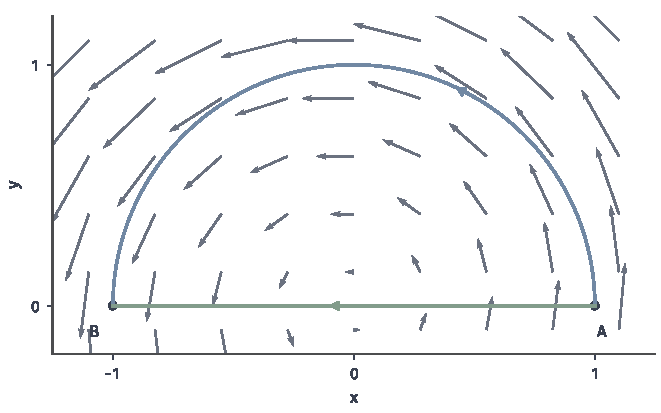
\includegraphics[width=112.0mm]{figures/01-mathematical-preliminaries-upper/01-mathematical-language-combinatorics-analysis-optimization/matplotlib/chapter3-concept-processes/rotation-field-paths.pdf}
 \caption{灰箭头为旋转场$F=(-y,x)^\top$，箭头长度统一缩放为实际场值的$1/4$。两条路径都从$A=(1,0)$到$B=(-1,0)$：蓝色上半圆与场同向，积分为$\pi$；绿色直径上场与位移垂直，积分为零。光滑性及相同端点不保证路径无关，下一小节将说明势函数给出的条件。}
 \label{fig:analysis-process-rotation-field-paths}
\end{figure}

\subsection{路径无关与势函数}
\label{sec:multivariable-potential-path-independence}

一般向量场的积分可能依赖整条路线。若向量场来自某个标量函数的梯度，链式法则就能把沿途累计化为端点变化；接下来分别说明这一结论、它的逆向判别以及定义域所需的条件。

\subsubsection{势函数与路径积分}

\paragraph{势函数}

寻找一个以向量场为梯度的标量函数，可以把做功解释成这个标量的变化。这样一个函数把每点的向量与整体端点差联系起来。
\begin{definition}[势函数]
设$U\subseteq\mathbb R^d$为非空开集，$\bm F:U\to\mathbb R^d$连续。
若存在$\phi\in C^1(U)$使$\bm F=\nabla\phi$，称$\phi$为$\bm F$的\term{势函数}（potential function），称$\bm F$为梯度场，也称保守场。
\end{definition}

例如$\phi(x,y)=x^2+y^2$给出$\bm F(x,y)=(2x,2y)^\top$；给势函数加常数不会改变该场。

\paragraph{路径积分基本定理}

将势函数与路径复合，就得到一个一元函数。它的导数恰是第二类路径积分中的被积函数，因此一元基本定理能恢复端点差。
\begin{theorem}[路径积分基本定理]
设$U\subseteq\mathbb R^d$为开集，$\phi\in C^1(U)$，$\gamma:[a,b]\to U$分段$C^1$。则
\begin{equation}
  \int_{\gamma}\nabla\phi\mathbin{\cdot}\mathrm{d}\bm{r}
  =\phi(\gamma(b))-\phi(\gamma(a)).
\label{eq:analysis-line-integral-gradient}
\end{equation}
\end{theorem}
\begin{proof}
在每个光滑参数段上，链式法则给出
\[
 (\phi\circ\gamma)'(t)=\nabla\phi(\gamma(t))^\top\gamma'(t).
\]
这个导数连续，所以对该段使用一元基本定理，积分等于该段两端的函数值之差。
对所有段相加，中间端点项逐一抵消，得到所述等式。
\end{proof}

因此梯度场的积分只依赖端点，任意闭路径上的积分都为零。方向反转使端点差变号，与前面的有向积分性质一致。

\subsubsection{路径无关的等价判别}

\paragraph{路径无关}

为了比较同一对端点间的不同路线，先要求域内任意两点能够由路径连接。欧氏开集若路径连通，任意两点之间也能选择域内的分段光滑路径。
\begin{definition}[路径无关]
设$U\subseteq\mathbb R^d$为非空、开且路径连通的集合，$\bm F:U\to\mathbb R^d$连续。
若对任意$\bm a,\bm b\in U$及域内从$\bm a$到$\bm b$的任意两条分段$C^1$路径，第二类路径积分都相等，称$\bm F$的路径积分与路径无关。
\end{definition}

势函数已给出路径无关的充分条件。反过来，若累计只由端点决定，就可以固定起点，用累计值定义势函数。
\begin{theorem}[路径无关的等价条件]
设$U\subseteq\mathbb R^d$非空、开且路径连通，$\bm F:U\to\mathbb R^d$连续。下列条件等价：
\begin{enumerate}
 \item 存在$\phi\in C^1(U)$使$\nabla\phi=\bm F$；
 \item $\bm F$的路径积分与路径无关；
 \item 域内每条分段$C^1$闭路径的积分都为零。
\end{enumerate}
\end{theorem}
\begin{proof}
条件1由路径积分基本定理推出条件2；条件2与常值闭路径比较，推出条件3。
若条件3成立，将两条同端点路径中的第二条反向，与第一条拼成闭路径，便得到两条原路径积分相等，因此条件3推出条件2。

最后假设条件2。固定$\bm a\in U$，用从$\bm a$到$\bm x$的路径积分定义$\phi(\bm x)$。
路径无关保证定义不依赖所选路线。由于$U$开，在$\bm x$附近可以沿第$j$个坐标追加一条足够短的线段，于是
\[
 \phi(\bm x+h\bm e_j)-\phi(\bm x)
 =\int_0^h F_j(\bm x+t\bm e_j)\,\mathrm dt.
\]
$F_j$连续，右侧除以$h$后趋于$F_j(\bm x)$，所以$\partial_j\phi=F_j$。
所有偏导数均连续，故$\phi\in C^1(U)$，得到条件1。
\end{proof}

\subsubsection{势函数存在的微分判别}

\paragraph{交叉偏导相等的必要条件}

已知势函数时，向量场各分量就是它的一阶偏导数。如果向量场本身为$C^1$，势函数便具有连续二阶偏导，混合偏导交换会给出可直接检查的条件。
\begin{theorem}[保守场的必要条件]
设$U\subseteq\mathbb R^d$为开集，$\bm F\in C^1(U;\mathbb R^d)$。
若$\bm F=\nabla\phi$，其中$\phi\in C^1(U)$，则对所有$i,j$和$\bm x\in U$，有
\[
 \partial_iF_j(\bm x)=\partial_jF_i(\bm x).
\]
\end{theorem}
\begin{proof}
由$\partial_j\phi=F_j\in C^1(U)$可知$\phi\in C^2(U)$，因此
$\partial_iF_j=\partial_i\partial_j\phi=\partial_j\partial_i\phi=\partial_jF_i$。
\end{proof}

\paragraph{星形域上的充分条件}

交叉偏导只比较局部变化，还需要域的条件才能据此构造全局势函数。一个便于直接计算的设定是星形开集：存在$\bm a\in U$，使从$\bm a$到每个$\bm x\in U$的整条线段都在$U$内；凸开集满足这一条件。
\begin{theorem}[星形域上势函数的构造]
设$U\subseteq\mathbb R^d$为关于$\bm a$星形的开集，$\bm F\in C^1(U;\mathbb R^d)$，且对所有$i,j$有$\partial_iF_j=\partial_jF_i$。则
\[
 \phi(\bm x)=\int_0^1\bm F(\bm a+t(\bm x-\bm a))^\top(\bm x-\bm a)\,\mathrm dt
\]
属于$C^1(U)$且满足$\nabla\phi=\bm F$。因此$\bm F$的路径积分与路径无关。
\end{theorem}
\begin{proof}
记$\bm z=\bm x-\bm a$。固定$\bm x$时，从$\bm a$到$\bm x$的线段是$U$内的紧集，因而其一个足够小的紧邻域仍在$U$内。
$\bm F$及其一阶偏导在这个邻域有界，所以可用参数积分的求导结论，在积分号下对第$j$个坐标求导。
交叉偏导条件将被积函数的导数化为
\[
 \begin{aligned}
 F_j(\bm a+t\bm z)+t\sum_i z_i\partial_jF_i(\bm a+t\bm z)
 &=F_j(\bm a+t\bm z)+t\sum_i z_i\partial_iF_j(\bm a+t\bm z)\\
 &=\frac{\mathrm d}{\mathrm dt}\bigl[tF_j(\bm a+t\bm z)\bigr].
 \end{aligned}
\]
积分后得到$\partial_j\phi(\bm x)=F_j(\bm x)$。这些偏导连续，所以$\phi\in C^1(U)$；路径无关由前一定理得到。
\end{proof}

域条件不能省略。例如在穿孔平面$\mathbb R^2\setminus\{\bm0\}$上，
\[
 \bm F(x,y)=\left(-\frac{y}{x^2+y^2},\frac{x}{x^2+y^2}\right)^\top
\]
满足$\partial_yF_1=\partial_xF_2=(y^2-x^2)/(x^2+y^2)^2$，却沿单位圆逆时针一周得到$2\pi$。
这个非零闭路径积分排除了全局势函数。局部导数相容，仍可能无法在整个定义域上把积分写为一个单值势函数的端点差。

\FloatBarrier

\par\Needspace{10\baselineskip}
\section{曲面积分}
\label{sec:analysis-surface-integration}

路径积分按长度累计细线上的量，曲面积分则按面积累计薄片上的量。
这里有两个不同的被积对象：标量函数$h:S\to\mathbb R$给出每单位面积的密度，
向量场$\bm F:S\to\mathbb R^3$给出空间中各点处有大小和方向的作用。
前者乘面积得到质量等总量；后者先取法向分量，再乘面积得到穿过曲面的通量。
二者都需要由参数化求出面积元，但只有通量需要选定法向。
本节先建立共同的曲面几何，再分别研究两类积分的定义、可积性、性质和计算。
全部积分采用勒贝格积分；参数曲面、面积元和通量的标准构造可参考\scite{math-openstax-calculus3}。

\subsection{参数曲面与面积}

空间中的曲面通常不能用一个平面区域直接代替，但可以用两个参数标记曲面上的点。
参数化的作用是把曲面上的累计转回二维参数域，同时用面积权重补偿曲面的倾斜和伸缩。

\subsubsection{曲面的参数化}

\paragraph{正则曲面片}

曲面的参数化是向量值映射：输入两个实数，输出三个空间坐标。
为了让它描述一张面，需要两个参数方向真正独立，并避免把同一片面重复计算。

\begin{definition}[正则参数曲面片]
\label{def:analysis-regular-surface-patch}
设$E\subseteq\mathbb R^2$是有界闭区域，$E=\overline{E^\circ}$且二维勒贝格测度$m_2(\partial E)=0$。
设$\bm r$在$E$的一个开邻域内是$C^1$映射，写成
\[
 \bm r(u,v)=(x(u,v),y(u,v),z(u,v))^\top\in\mathbb R^3.
\]
若不同参数只有在都属于$\partial E$时才允许表示同一点，
且两个偏导向量$\bm r_u,\bm r_v$在$E^\circ$上处处线性无关，则称$\bm r$为一个正则曲面片的参数化，曲面片记为$S=\bm r(E)$。
参数边界允许产生接缝或退化点；这些边界部分按零曲面面积处理。
\end{definition}

这里两个切向量线性无关，是指对任意实数$\alpha,\beta$，
$\alpha\bm r_u+\beta\bm r_v=\bm0$只有在$\alpha=\beta=0$时才成立。

固定$v$而改变$u$得到一条参数曲线，它的速度是$\bm r_u$；固定$u$得到的另一条参数曲线的速度是$\bm r_v$。
二者张成曲面的切平面。这里$\bm r_u,\bm r_v$都是三维向量，
并非某个标量函数的两个偏导数。
例如$\bm r(u,v)=(u,v,u+v)^\top$、$E=[0,1]^2$描述平面$z=x+y$上的一块平行四边形，
两个切向量分别为$(1,0,1)^\top$和$(0,1,1)^\top$。

\paragraph{叉积}

小参数矩形的两条边近似映为$\bm r_u\Delta u$和$\bm r_v\Delta v$。
要求它们张成的平行四边形面积，需要一个同时记录面积和垂直方向的向量运算。
对$\bm a,\bm b\in\mathbb R^3$，定义叉积
\[
 \bm a\times\bm b
 =(a_2b_3-a_3b_2,\ a_3b_1-a_1b_3,\ a_1b_2-a_2b_1)^\top.
\]
它垂直于$\bm a,\bm b$，长度等于两向量张成的平行四边形面积，交换次序则变号。
因此正则性也可以写成$\bm r_u\times\bm r_v\ne\bm0$，
小曲面片的面积近似为$\lVert\bm r_u\times\bm r_v\rVert_2\Delta u\Delta v$。

\subsubsection{曲面面积的表示}

\paragraph{面积元与面积测度}

参数域上的面积$\mathrm du\,\mathrm dv$与曲面上的实际面积通常不同。
把刚才得到的局部面积比作为权重，就能把二维勒贝格测度转成曲面上的面积测度。

\begin{definition}[曲面面积测度]
\label{def:analysis-surface-area-measure}
在上述曲面片上，记$J_S(u,v)=\lVert\bm r_u\times\bm r_v\rVert_2$。
若$A\subseteq S$的原像$\bm r^{-1}(A)\cap E$勒贝格可测，则称$A$为曲面可测集，定义
\[
 \sigma_S(A)=\iint_E\bm1_A(\bm r(u,v))J_S(u,v)\,\mathrm du\,\mathrm dv.
\]
曲面面积元记为$\mathrm dS$，参数表示为
\[
 \mathrm dS=J_S(u,v)\,\mathrm du\,\mathrm dv,
 \qquad \operatorname{area}(S)=\sigma_S(S).
\]
\end{definition}

原像保留集合的补、交和并，而右侧是非负权重下的勒贝格积分，
所以这些曲面可测集构成$\sigma$代数，$\sigma_S$在其上可数可加。
$J_S$在紧集$E$上连续有界，且$m_2(E)<\infty$，故这里的曲面片面积有限。
参数边界的二维测度为零，不贡献面积；边界接缝上的重复参数也不重复累计正面积部分。
前面的斜平面片有$\bm r_u\times\bm r_v=(-1,-1,1)^\top$，
故$J_S=\sqrt3$，其面积为$\sqrt3$，而参数正方形的面积为$1$。


图~\ref{fig:analysis-process-surface-area-stretch}将参数小块与实际斜面小块对应起来，解释叉积长度校正的是哪一个面积。
\begin{figure*}[!htbp]
 \centering
 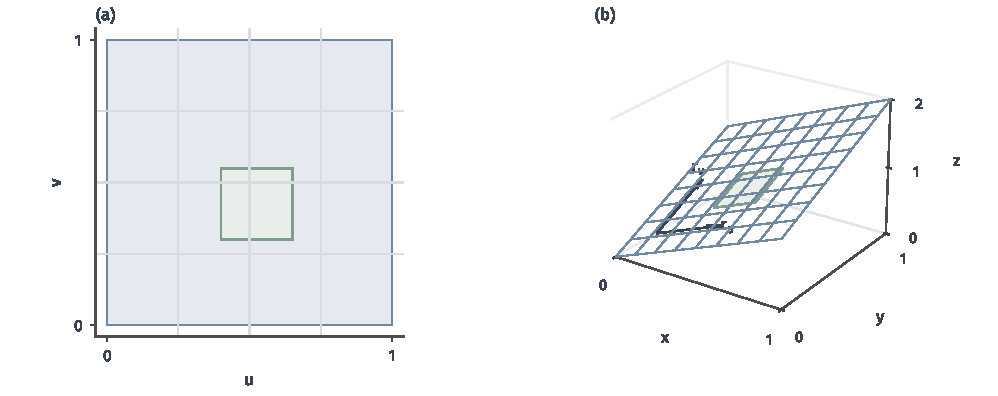
\includegraphics[width=169.0mm]{figures/01-mathematical-preliminaries-upper/01-mathematical-language-combinatorics-analysis-optimization/matplotlib/chapter3-concept-processes/surface-area-stretch.pdf}
 \caption{参数化$r(u,v)=(u,v,u+v)^\top$把单位正方形映为斜平面片，绿色块为同一参数子区间及其像。两切向量$r_u=(1,0,1)^\top$、$r_v=(0,1,1)^\top$在右侧按$0.4$倍画出，叉积长度为$\sqrt3$。每个参数面积都放大$\sqrt3$倍，故不能把$\mathrm du\,\mathrm dv$直接当成$\mathrm dS$。}
 \label{fig:analysis-process-surface-area-stretch}
\end{figure*}

\paragraph{重参数化}

同一块面可以用不同参数标记。要让上面的面积描述曲面本身，
还需证明更换单次覆盖的参数后，面积权重恰好抵消参数域的面积变化。

\begin{theorem}[重参数化下的面积元]
\label{thm:analysis-surface-reparameterization}
设$\bm r:E\to S$满足上述条件，$T:\widetilde E\to E$是参数域之间的双射，
在闭域的开邻域内为$C^1$映射，并在内部是$C^1$微分同胚。
若$\widetilde{\bm r}=\bm r\circ T$仍满足曲面片条件，则
\[
 \begin{aligned}
 \widetilde{\bm r}_\xi\times\widetilde{\bm r}_\eta
 &=\det\bm J_T\,(\bm r_u\times\bm r_v)\circ T,\\
 \widetilde J_S&=(J_S\circ T)|\det\bm J_T|.
 \end{aligned}
\]
两组参数由此给出同一面积测度。
\end{theorem}

\begin{proof}
链式法则给出$\widetilde{\bm r}_\xi=\bm r_u u_\xi+\bm r_v v_\xi$和
$\widetilde{\bm r}_\eta=\bm r_u u_\eta+\bm r_v v_\eta$，其中右端各量在$T(\xi,\eta)$处取值。
利用叉积的双线性、$\bm a\times\bm a=\bm0$和交换次序变号，得到
\[
 \widetilde{\bm r}_\xi\times\widetilde{\bm r}_\eta
 =(u_\xi v_\eta-v_\xi u_\eta)(\bm r_u\times\bm r_v)\circ T.
\]
取长度得到第二式。将它代入任一可测集$A$的面积定义，
二维勒贝格积分的换元公式便把新参数下的积分变回原积分。
\end{proof}

行列式的绝对值保证面积非负；行列式本身的符号则记录参数次序是否翻转，
后面选取通量的法向时还会使用这一信息。
若参数在正面积范围内重复覆盖，参数积分会重复累计，不能直接把它当作单次曲面面积。

\paragraph{分片曲面}

球面、封闭边界或带折角的曲面可能需要多张参数片描述。
本节处理有限分片的情形：各片内部不重叠，交接部分在相邻曲面片中面积均为零，
整个曲面的面积测度由各片面积测度相加。
这样曲面面积和后面的面积积分都可以逐片计算，不需在接缝上补加一项。
无界曲面或不能由这里的有限正则片覆盖的曲面，还需另外处理覆盖和可积性条件。

\subsection{第一类曲面积分}

给定曲面以后，先考虑标量函数$h$在曲面上的累计。
面积测度已经确定了每块薄片的权重，因此可以直接沿用前面建立的测度积分。

\subsubsection{积分的定义和可积性}

\paragraph{按面积的积分}

把面密度乘小片面积再相加，提示我们应当对面积测度积分。
下面的定义既包含连续密度，也允许有跳跃或仅可测的密度。

\begin{definition}[第一类曲面积分]
\label{def:analysis-scalar-surface-integral}
设$h$是$S$上的可测标量函数。
当$h\geq0$时，定义它的\term{第一类曲面积分}（scalar surface integral）为
\begin{equation}
 \int_Sh\,\mathrm dS
 =\iint_Eh(\bm r(u,v))J_S(u,v)\,\mathrm du\,\mathrm dv.
 \label{eq:analysis-scalar-surface-integral}
\end{equation}
该值允许为$+\infty$。一般实值$h$在$\int_S|h|\,\mathrm dS<\infty$时称为曲面可积，
其积分按正、负部分之差定义，仍满足上式。
\end{definition}

取$h=1$得到面积，取非负面密度得到质量。
在前面的单位参数斜平面片上，常数密度$h=2$给出
\[
 \int_S2\,\mathrm dS=\int_0^1\int_0^1 2\sqrt3\,\mathrm du\,\mathrm dv=2\sqrt3.
\]
这一累计不使用法向，因此把曲面的朝向反过来不会改变结果。

\paragraph{可积性的要求}

积分是否有限，取决于函数大小和曲面面积权重共同作用后的累计。
由定义，$h$曲面可积当且仅当参数函数可测且
\[
 \iint_E|h(\bm r(u,v))|J_S(u,v)\,\mathrm du\,\mathrm dv<\infty.
\]
连续函数是一个便于验证的充分情形：$S=\bm r(E)$紧致，连续的$h$有界，
因而$\int_S|h|\,\mathrm dS\leq \sup_S|h|\,\sigma_S(S)<\infty$。
可测性本身并不保证这个绝对积分有限；如果函数在某处无界，仍须检验上式。
这些条件相对于曲面面积，而非三维体积测度；曲面在三维空间中体积为零，并不使面积积分为零。

\subsubsection{积分的性质}

两类标量密度可以叠加，也可以把曲面分开累计。
这些运算由面积测度上的勒贝格积分给出，以下均以相应函数曲面可积为前提。

\paragraph{加法}

对曲面可积的$h,k$，$h+k$也可积，而且
\[
 \int_S(h+k)\,\mathrm dS=\int_Sh\,\mathrm dS+\int_Sk\,\mathrm dS.
\]
可积性由$|h+k|\leq|h|+|k|$得到，等式来自标量勒贝格积分的加法性质。

\paragraph{减法}

对曲面可积的$h,k$，$h-k$也可积，而且
\[
 \int_S(h-k)\,\mathrm dS=\int_Sh\,\mathrm dS-\int_Sk\,\mathrm dS.
\]
这里$|h-k|\leq|h|+|k|$保证绝对可积，等式来自标量勒贝格积分的减法性质。

\paragraph{数乘}

对实数$c$和曲面可积的$h$，$ch$曲面可积，且
\[
 \int_Sch\,\mathrm dS=c\int_Sh\,\mathrm dS.
\]
因为$|ch|=|c||h|$，绝对积分仍有限；数乘公式与参数域上的数乘公式一致。

\paragraph{曲面分割的可加性}

若可测子集$A_j\subseteq S$两两不交，且$h$在$S$上曲面可积，则
\[
 \int_{\bigcup_{j=1}^\infty A_j}h\,\mathrm dS
 =\sum_{j=1}^\infty\int_{A_j}h\,\mathrm dS.
\]
右侧绝对收敛，因为其各项绝对值之和不超过$\int_S|h|\,\mathrm dS$。
有限分片曲面的求和是这一性质的特例；仅在零面积接缝上相交也不影响等式。

\paragraph{单调性}

若曲面可积的$h,k$满足$h\leq k$在曲面面积意义下几乎处处成立，则
\[
 \int_Sh\,\mathrm dS\leq\int_Sk\,\mathrm dS.
\]
因为$k-h$几乎处处非负，其积分非负，应用减法公式即可得到这一不等式。
这里的“几乎处处”允许忽略零曲面面积集合。它不以三维体积衡量例外集合。

\paragraph{绝对值不等式}

对任一曲面可积的$h$，将单调性应用于$-|h|\leq h\leq|h|$得到
\[
 \left|\int_Sh\,\mathrm dS\right|\leq\int_S|h|\,\mathrm dS.
\]
因此绝对值的面积积分给出了原积分大小的上界。

\subsubsection{积分的计算}

计算第一类曲面积分时，先选单次覆盖的参数化，再把$h$与参数化复合，并乘叉积的长度。
若曲面是标量函数$z=\psi(x,y)$在参数域$D$上的图像，
其中$D$满足本节的有界闭域和零测边界条件，$\psi$在$D$的开邻域内为$C^1$，可以直接取
$\bm r(x,y)=(x,y,\psi(x,y))^\top$。计算得
\[
 \bm r_x\times\bm r_y=(-\psi_x,-\psi_y,1)^\top,
\]
所以对曲面可积的$h$有
\[
 \int_Sh\,\mathrm dS
 =\iint_Dh(x,y,\psi(x,y))\sqrt{1+\psi_x^2+\psi_y^2}\,\mathrm dx\,\mathrm dy.
\]
根号校正倾斜造成的面积增长。例如$z=ax+by+c$在单位圆盘上方的部分面积为
$\pi\sqrt{1+a^2+b^2}$。若无法向同一坐标平面单值投影，则需换参数化或分片。

半径$R>0$的球面可以取参数
\[
 \begin{gathered}
 \bm r(\varphi,\theta)
 =(R\sin\varphi\cos\theta,R\sin\varphi\sin\theta,R\cos\varphi)^\top,\\
 0\leq\varphi\leq\pi,\quad 0\leq\theta\leq2\pi.
 \end{gathered}
\]
参数域内部正则且单次覆盖，叉积长度为$R^2\sin\varphi$。
两极与经线接缝来自参数边界，不贡献面积；不用在两极把叉积归一化。
因此
\[
 \operatorname{area}(S)
 =\int_0^{2\pi}\int_0^\pi R^2\sin\varphi\,\mathrm d\varphi\,\mathrm d\theta
 =4\pi R^2.
\]

\subsection{第二类曲面积分}

现在改变被积对象，考虑向量场$\bm F:S\to\mathbb R^3$穿过曲面的累计。
面积只给出小片的大小，尚未规定“穿过”的正方向；要取法向分量，必须先选定曲面的朝向。

\subsubsection{曲面的定向}

\paragraph{单位法向量}

正则点的切平面有两个相反的单位法向量，选择哪一个决定通量的正负。
参数次序提供一个局部选择：在$E^\circ$上令
\[
 \bm n(\bm r(u,v))
 =\frac{\bm r_u\times\bm r_v}{\lVert\bm r_u\times\bm r_v\rVert_2}.
\]
这个向量长度为$1$，并且垂直于两个参数方向；交换$u,v$会把它反转。
参数边界上若叉积退化，不使用这个商定义法向。该部分面积为零，不影响通量积分。

\paragraph{定向与可定向性}

每一点分别选择正负还不够，选择需要在一张面上相容。
相容的连续选择使相邻位置的正方向保持一致，这就是曲面的定向。

\begin{definition}[曲面的定向]
\label{def:analysis-surface-orientation}
在光滑曲面$S$上连续选取一个单位法向量场$\bm n$，称为给曲面\term{定向}（orientation）。
存在这种选择的曲面称为可定向曲面；$\bm n$和$-\bm n$给出相反的定向。
分片光滑曲面要求各片的选择相容：光滑接合处选择同一侧法向，
折角处按整个曲面的同一侧约定，但不要求接缝上存在唯一法向。
\end{definition}

例如图像曲面可以选向上法向，球面可以选外法向。
闭曲面围成规则区域时，外法向指向区域外侧。
不能在全曲面相容选择法向时，面积积分仍有定义，但不能使用这里的全局定向通量。

\subsubsection{积分的定义和可积性}

\paragraph{通量积分}

选定$\bm n$以后，$\bm F^\top\bm n$是一个标量：它表示场沿法向穿过单位面积的分量。
对这个标量作面积积分，就得到有正负号的通量。

\begin{definition}[第二类曲面积分]
\label{def:analysis-surface-flux-integral}
设可定向曲面$S$已选定单位法向$\bm n$，向量场$\bm F:S\to\mathbb R^3$的法向分量可测，且
$\int_S|\bm F^\top\bm n|\,\mathrm dS<\infty$。
定义\term{第二类曲面积分}（flux integral），也称通量积分，为
\begin{equation}
 \int_S\bm F^\top\bm n\,\mathrm dS
 =\iint_E\bm F(\bm r(u,v))^\top(\bm r_u\times\bm r_v)\,\mathrm du\,\mathrm dv,
 \label{eq:analysis-surface-flux}
\end{equation}
其中参数化的叉积方向须与所选$\bm n$一致；若方向相反，右端需乘$-1$。
分片曲面的通量按相容定向逐片相加。
\end{definition}

通量为正表示沿所选法向的净贡献，为负表示逆法向的净贡献。
它的结果是一个标量，不能与向量场三个分量分别作面积积分所得的向量混为一谈。
若$\bm F=(P,Q,R)^\top$，有向面积分量也可记为
\[
 \bm n\,\mathrm dS=(\mathrm dy\,\mathrm dz,\mathrm dz\,\mathrm dx,\mathrm dx\,\mathrm dy)^\top,
\]
从而把通量写为$\int_SP\,\mathrm dy\,\mathrm dz+Q\,\mathrm dz\,\mathrm dx+R\,\mathrm dx\,\mathrm dy$。
这些分量代表有向投影面积，其符号由法向决定。


图~\ref{fig:analysis-process-normal-projection}在一个法向截面内分解场值，说明通量只累计哪一部分。
\begin{figure}[!htbp]
 \centering
 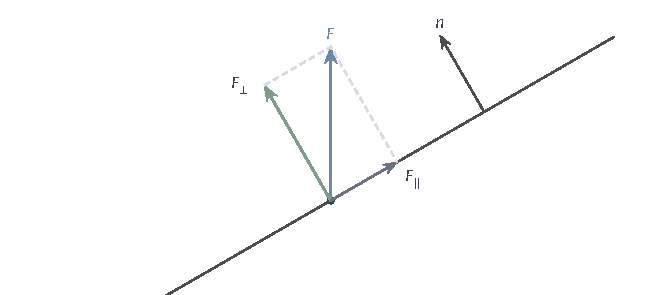
\includegraphics[width=112mm]{figures/01-mathematical-preliminaries-upper/01-mathematical-language-combinatorics-analysis-optimization/tikz/chapter3-concept-processes/normal-projection.pdf}
 \caption{黑斜线表示局部切平面的一个截面，$n$为所选单位法向。向量$F$分为$F_\perp=(F^\top n)n$与切向部分$F_\parallel$；通量使用有符号标量$F^\top n$乘面积，切向部分不贡献。将$n$改为$-n$时标量分量变号，但投影向量$F_\perp$不变，这与直接把场反向不同。}
 \label{fig:analysis-process-normal-projection}
\end{figure}

\paragraph{可积性的要求}

通量只累计法向分量，因此其有限可积性的准确条件是
\[
 \iint_E
 \left|\bm F(\bm r(u,v))^\top(\bm r_u\times\bm r_v)\right|
 \,\mathrm du\,\mathrm dv<\infty.
\]
一个更容易验证的充分条件是$\int_S\lVert\bm F\rVert_2\,\mathrm dS<\infty$。
因为$\lVert\bm n\rVert_2=1$，Cauchy--Schwarz不等式给出
$|\bm F^\top\bm n|\leq\lVert\bm F\rVert_2$。
连续向量场在本节的紧致有限分片曲面上有界，因而满足这一充分条件。
切向分量不进入通量，所以不能把法向分量可积与向量场各分量都可积视为同一个条件。

\subsubsection{积分的性质}

以下运算都在同一曲面、同一法向约定下进行，并假定各法向分量可积。
它们可归结为标量函数$\bm F^\top\bm n$的面积积分，但方向变化需要单独说明。

\paragraph{加法}

向量场相加以后，其法向分量也相加，因此
\[
 \begin{aligned}
 \int_S(\bm F+\bm G)^\top\bm n\,\mathrm dS
 &=\int_S\bm F^\top\bm n\,\mathrm dS\\
 &\quad{}+\int_S\bm G^\top\bm n\,\mathrm dS.
 \end{aligned}
\]
绝对可积性由两项法向分量的绝对值之和控制，积分等式来自标量面积积分的加法性质。

\paragraph{减法}

向量场相减以后，其法向分量也相减，因此
\[
 \begin{aligned}
 \int_S(\bm F-\bm G)^\top\bm n\,\mathrm dS
 &=\int_S\bm F^\top\bm n\,\mathrm dS\\
 &\quad{}-\int_S\bm G^\top\bm n\,\mathrm dS.
 \end{aligned}
\]
两项法向分量绝对可积时，它们的差仍绝对可积，积分等式来自标量面积积分的减法性质。

\paragraph{数乘}

实数$c$可以提出积分号，原因是$(c\bm F)^\top\bm n=c(\bm F^\top\bm n)$，即
\[
 \int_S(c\bm F)^\top\bm n\,\mathrm dS
 =c\int_S\bm F^\top\bm n\,\mathrm dS.
\]
这里缩放的是场，曲面的法向约定保持固定。

\paragraph{曲面分割的可加性}

将$S$分为内部不重叠的有限片$S_1,\ldots,S_N$，并在每片采用原定向的限制，则
\[
 \int_S\bm F^\top\bm n\,\mathrm dS
 =\sum_{j=1}^N\int_{S_j}\bm F^\top\bm n\,\mathrm dS.
\]
零面积接缝不贡献积分；若某片单独反转法向，就改变了被累计的符号，不能仍按同一定向求和。

\paragraph{法向反转}

在场和曲面不变时，把$\bm n$换成$-\bm n$会使通量变号：
\[
 \int_S\bm F^\top(-\bm n)\,\mathrm dS
 =-\int_S\bm F^\top\bm n\,\mathrm dS.
\]

\paragraph{重参数化}

更换参数时，保持已选定的几何法向。重参数化定理表明，参数叉积多出$\det\bm J_T$，
而区域换元使用$|\det\bm J_T|$；若变换翻转参数方向，必须同时校正叉积相对于所选法向的符号。
固定曲面的定向并完成这一校正，通量便与参数选择无关。

\subsubsection{积分的计算}

计算通量时，先固定法向，再选与之相容的参数化，最后累计$\bm F$与有向面积向量的内积。
对于图像曲面$z=\psi(x,y)$，前面已求出叉积$(-\psi_x,-\psi_y,1)^\top$，它的第三分量为正。
因此取向上法向时，对$\bm F=(P,Q,R)^\top$有
\[
 \int_S\bm F^\top\bm n\,\mathrm dS
 =\iint_D(-P\psi_x-Q\psi_y+R)(x,y,\psi(x,y))\,\mathrm dx\,\mathrm dy.
\]
取向下法向则在右侧加负号。这一式直接使用有向面积，不能再额外乘一次叉积长度。

在平面片$\bm r(u,v)=(u,v,u+v)^\top$上，向上单位法向为$(-1,-1,1)^\top/\sqrt3$。
对竖直单位场$\bm F=(0,0,1)^\top$，场与参数叉积的内积为$1$，故
\[
 \int_S\bm F^\top\bm n\,\mathrm dS
 =\int_0^1\int_0^1 1\,\mathrm du\,\mathrm dv=1.
\]
其面积为$\sqrt3$，但法向分量只有$1/\sqrt3$。
同样地，平面$z=ax+by+c$在单位圆盘上方的部分对该场的向上通量为$\pi$，
等于水平投影面积；它的实际面积则为$\pi\sqrt{1+a^2+b^2}$。

对半径$R$的球面，前面采用$(\varphi,\theta)$次序的参数叉积指向外侧。
若$\bm F(\bm x)=\bm x/R$，则球面上的$\bm F$恰等于外单位法向，故
\[
 \int_S\bm F^\top\bm n\,\mathrm dS
 =\int_S1\,\mathrm dS=4\pi R^2.
\]
内向通量为$-4\pi R^2$。这次面积与外向通量相等，是因为法向分量处处为$1$；
下一节再用空间区域内部的散度累计核对同一个通量。

\FloatBarrier

\section{三类积分之间的关系}
\label{sec:multivariable-boundary-relations}

一元微积分基本定理把导数在区间上的积分化为两个端点的函数值之差。
区域、路径和曲面积分也有类似关系：特定导数在内部的积分，可以化为原函数或原向量场在边界上的积分。
本节分别回答三个问题：平面区域积分何时等于边界路径积分，空间区域积分何时等于边界曲面积分，曲面积分何时等于边界路径积分。

这些关系中的被积对象不能互换。路径环流累计向量场的切向分量，通量累计向量场的法向分量；
相应的内部积分分别使用旋度或散度。下面先明确这些导数的输入与输出，以及边界方向的约定，再给出各公式的条件与推导。
所有区域积分以及路径、曲面的参数积分均采用勒贝格积分。经典公式的组织参考向量微积分教材\scite{math-openstax-calculus3}。

\subsection{积分公式中的微分算子}

前面已用梯度表示多元标量函数的一阶变化。现在给定开集$U$上的向量场$\bm F$，我们关心它的各分量怎样共同产生净流出或环流。
这两个问题需要不同的偏导数组合。先介绍以向量场为输入的散度与旋度，再介绍以标量函数为输入的Laplace算子，分别明确它们的输出类型。

\subsubsection{散度}

对一个小长方体，沿每个坐标方向流出的量与流入的量之差，取决于向量场在该方向上的分量怎样变化。
把各坐标方向的变化率相加，就得到描述局部净流出的标量。
\begin{definition}[散度]
\label{def:multivariable-divergence}
设$U\subseteq\mathbb R^d$为开集，$\bm F=(F_1,\ldots,F_d)^\top:U\to\mathbb R^d$的各分量一阶偏导数存在。
$\bm F$的\term{散度}（divergence）是标量函数
\[
 \operatorname{div}\bm F
 =\nabla\mathbin{\cdot}\bm F
 =\sum_{j=1}^d\partial_jF_j.
\]
\end{definition}
三维径向场$\bm F(x,y,z)=(x,y,z)^\top$的散度是$1+1+1=3$；
旋转场$\bm G(x,y,z)=(-y,x,0)^\top$的散度是$0$。
散度为零表示局部净流出率为零，并不表示向量场为零。
二维场$(P,Q)^\top$的散度相应为$P_x+Q_y$，后面的平面通量公式使用这一标量函数。

\subsubsection{旋度}

净流出不能描述绕一点旋转的运动：上面的旋转场散度为零，沿圆周的环流却不为零。
在三维空间中，需要分别记录绕三个坐标方向的局部环流率，并把它们组成一个向量。
\begin{definition}[旋度]
\label{def:multivariable-curl}
设$U\subseteq\mathbb R^3$为开集，$\bm F=(F_1,F_2,F_3)^\top:U\to\mathbb R^3$的各分量一阶偏导数存在。
$\bm F$的\term{旋度}（curl）是向量场
\[
 \operatorname{curl}\bm F=\nabla\times\bm F
 =\begin{pmatrix}
   \partial_yF_3-\partial_zF_2\\
   \partial_zF_1-\partial_xF_3\\
   \partial_xF_2-\partial_yF_1
  \end{pmatrix}.
\]
\end{definition}
例如$\bm F=(-y/2,x/2,0)^\top$的旋度为$(0,0,1)^\top$，径向场$(x,y,z)^\top$的旋度为零。
旋度沿某一单位法向的分量，描述垂直于该方向的小曲面上的局部环流率；后面的Stokes公式把这一关系写成积分等式。

对二维场$(P,Q)^\top$，平面内需要的是标量$Q_x-P_y$。
将它补零写成三维场$(P,Q,0)^\top$后，这一标量正是旋度的第三分量，因而与向上法向相对应。
符号$\nabla\mathbin\cdot$和$\nabla\times$表示这里定义的偏导数组合，不是两个普通数值向量的内积或叉积。


图~\ref{fig:analysis-process-divergence-circulation-fields}在同一个单位圆周上分别观察净流出与切向环流，比较两种微分算子所记录的信息。
\begin{figure*}[!htbp]
 \centering
 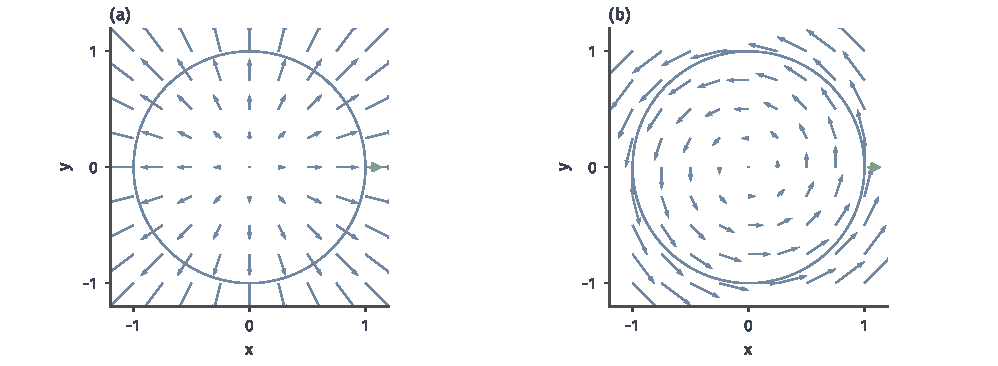
\includegraphics[width=169.0mm]{figures/01-mathematical-preliminaries-upper/01-mathematical-language-combinatorics-analysis-optimization/matplotlib/chapter3-concept-processes/divergence-circulation-fields.pdf}
 \caption{(a) 径向场$(x,y)^\top$的二维散度为$2$、旋转率$Q_x-P_y=0$，圆周外向通量为$2\pi$、环流为零。(b) 旋转场$(-y,x)^\top$的散度为零、旋转率为$2$，通量为零、环流为$2\pi$。绿箭头仅标记外法向；蓝色场箭头按相同常数缩放。零散度不等于零场，也不等于零环流。}
 \label{fig:analysis-process-divergence-circulation-fields}
\end{figure*}

\subsubsection{Laplace算子}

标量函数的梯度是向量场，因此可以继续取散度，把各坐标方向的二阶变化相加。
这一复合运算在多元分部积分中出现，仍以标量函数作为输入与输出。
\begin{definition}[Laplace算子]
\label{def:multivariable-laplacian}
对开集$U\subseteq\mathbb R^d$上的二阶连续可微标量函数$v$，定义\term{Laplace算子}（Laplacian）为
\[
 \Delta v=\operatorname{div}(\nabla v)
 =\sum_{j=1}^d\partial_j^2v.
\]
\end{definition}
例如$v(x,y,z)=x^2+y^2+z^2$时，$\Delta v=6$。
梯度将标量函数变为向量场，散度将向量场变为标量函数；不能将$\Delta v$与向量场的旋度混为同一类对象。

\subsection{边界的定向}

将一个区域分成相邻小块时，公共边或公共面不属于原区域的外边界。
要使这些内部贡献相消，各小块必须采用相容的方向。不同几何对象的方向约定如下。

\subsubsection{平面区域的正向边界}

平面区域的边界是路径，所以先规定沿边界行进的方向。简单闭曲线指除首尾相合外不自交的闭曲线。
对有界平面区域，取边界方向使沿曲线前进时区域总在左侧，称为正向边界。
外边界因此逆时针，围绕孔洞的内边界顺时针。例如圆环$1<x^2+y^2<4$的两圈边界必须取相反方向。

边界由多段光滑弧组成时，按这一方向逐段相接，转角处不另加积分项。
相邻平面小块各自采用正向边界时，共同边被沿相反方向走过，两个有向路径积分恰好抵消。

\subsubsection{区域边界的外法向}

通量需要的是法向，而不是边界的行进方向。空间区域的外单位法向从内部指向外部；
有孔洞时，孔洞边界的外法向指向孔洞。相邻子区域的公共面上，各自的外法向相反，所以内部通量相消。
二维区域边界上的外单位法向也按同样方式规定，但积分按弧长累计。

\subsubsection{定向曲面边界的诱导方向}

曲面取定单位法向$\bm n$后，其边界路径的方向不能再任意选择。
边界正向按右手约定确定：右手大拇指朝法向，其余手指弯曲的方向为正向。
等价地，沿边界前进并把头朝向法向时，曲面留在左侧。向上定向的平面圆盘，其边界从上方看为逆时针。

若翻转曲面法向，边界的诱导方向也随之翻转。分片曲面的定向相容，指相邻曲面片在公共边上诱导出相反的行进方向。
这时公共边上的路径积分相消，只留下整张曲面的真正边界。


图~\ref{fig:analysis-process-boundary-orientation-cancellation}把相容方向的作用画出来：内边相消，才会只剩整个对象的外边界。
\begin{figure}[!htbp]
 \centering
 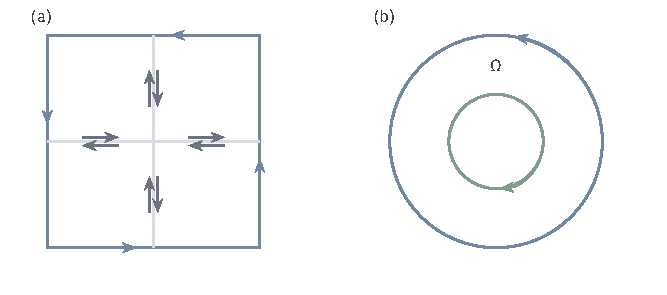
\includegraphics[width=112mm]{figures/01-mathematical-preliminaries-upper/01-mathematical-language-combinatorics-analysis-optimization/tikz/chapter3-concept-processes/boundary-orientation-cancellation.pdf}
 \caption{(a) 四个小正方形各取逆时针正向，共同边被沿相反方向走过；灰箭头略错开以便辨认，实际是同一条边。相加后只留下蓝色外边界。(b) 圆环的外边界逆时针、孔洞边界顺时针，沿任一边界前进时区域均在左侧。曲面拼片时也按公共边相反方向保证Stokes边界项相消。}
 \label{fig:analysis-process-boundary-orientation-cancellation}
\end{figure}

\subsection{平面区域积分与边界路径积分}

在平面上，区域的边界是一维路径。对同一个二维向量场，可以沿边界累计切向作用，也可以累计法向通量；
两种边界积分分别对应区域内部不同的偏导数组合。

\subsubsection{Green公式的环流形式}

沿正向边界的切向路径积分描述环流。它所对应的内部量是$Q_x-P_y$，而不是散度$P_x+Q_y$。
下面的公式把二者联系起来，并明确区域、场与方向的条件。
\begin{theorem}[Green公式]
\label{thm:multivariable-green}
设$\Omega\subseteq\mathbb R^2$为有界开区域，边界由有限条分段$C^1$简单闭曲线组成，
且区域在每段光滑边界附近位于边界的一侧。边界取正向，即外边界逆时针、孔洞边界顺时针。
若二维向量场$\bm F=(P,Q)^\top$在$\overline\Omega$的开邻域内连续可微，则\term{Green公式}（Green's theorem）给出
\begin{equation}
 \oint_{\partial\Omega}P\,\mathrm dx+Q\,\mathrm dy
 =\iint_\Omega\left(\frac{\partial Q}{\partial x}-\frac{\partial P}{\partial y}\right)\,\mathrm dx\,\mathrm dy.
 \label{eq:multivariable-green}
\end{equation}
\end{theorem}
左侧是向量场的切向路径积分；右侧是标量函数$Q_x-P_y$的区域积分。
在矩形上，二者的等式可以直接由一元基本定理和Fubini定理推出。
\begin{proof}[矩形情形的证明]
取$\Omega=(a,b)\times(c,d)$。场在闭矩形附近连续可微，以下被积函数均可积，故
\[
 \begin{aligned}
 -\iint_\Omega\partial_yP\,\mathrm dx\,\mathrm dy
 &=\int_a^b[P(x,c)-P(x,d)]\,\mathrm dx,\\
 \iint_\Omega\partial_xQ\,\mathrm dx\,\mathrm dy
 &=\int_c^d[Q(b,y)-Q(a,y)]\,\mathrm dy.
 \end{aligned}
\]
第一行对应下边从左向右、上边从右向左的两项积分，第二行对应右边从下向上、左边从上向下的两项积分。
四项合起来，正是沿下、右、上、左四条边逆时针行进得到的路径积分。
\end{proof}
有限个矩形拼接时，公共边上的积分因方向相反而抵消。
一般规则区域的证明还需处理区域分片及边界逼近误差，不能仅凭小矩形上的等式完成；这里引用一般形式，完整论证可参考向量微积分教材\scite{math-strang1991calculus}。

取$\bm F=(-y,x)^\top$、$\Omega$为单位圆盘，右侧被积函数为$2$，所以边界环流为$2\pi$。
这与直接参数化圆周得到的结果一致，也说明正向约定决定了结果的符号。

\subsubsection{Green公式的通量形式}

要计算穿过平面区域边界的净通量，需要把场投影到外法向上。
沿正向边界，单位切向量顺时针转过直角就得到外单位法向，因此它们的有向弧长分量满足
\[
 \bm n\,\mathrm ds=(\mathrm dy,-\mathrm dx)^\top.
\]
这一关系将法向通量转化为可以使用Green公式的路径积分。
\begin{theorem}[平面区域的通量公式]
\label{thm:multivariable-planar-flux}
在Green公式相同的区域条件下，若$\bm F=(F_1,F_2)^\top$在$\overline\Omega$的开邻域内连续可微，
$\bm n$是边界的外单位法向，则
\[
 \int_{\partial\Omega}\bm F^\top\bm n\,\mathrm ds
 =\iint_\Omega\operatorname{div}\bm F\,\mathrm dx\,\mathrm dy.
\]
\end{theorem}
\begin{proof}
利用外法向与正向边界的关系，左侧等于
$\oint_{\partial\Omega}(-F_2)\,\mathrm dx+F_1\,\mathrm dy$。
在Green公式中取$(P,Q)=(-F_2,F_1)$，右侧即为$\partial_xF_1+\partial_yF_2=\operatorname{div}\bm F$的区域积分。
\end{proof}
这也是二维的散度公式。它与环流形式使用相同的区域条件，但累计的边界分量和内部导数不同。

例如单位圆盘上的$\bm F(x,y)=(x,y)^\top$有散度$2$，区域积分为$2\pi$。
边界参数化为$\bm\gamma(t)=(\cos t,\sin t)^\top$，$0\leq t\leq2\pi$，
外法向$\bm n=\bm\gamma(t)$，$\mathrm ds=\mathrm dt$，且$\bm F^\top\bm n=1$，所以边界通量也为$2\pi$。
若改取内法向，通量就变为$-2\pi$。
相比之下，旋转场$(-y,x)^\top$的散度为零，在圆周上与法向垂直，通量为零；它的环流却是前面算出的$2\pi$。

\subsection{空间区域积分与边界曲面积分}

将平面区域换成三维空间区域后，边界从曲线变成闭曲面。
对应关系仍然是内部散度的积分等于边界净通量；这一关系还可以推出多元函数的分部积分公式。

\subsubsection{Gauss公式}

一个小长方体的两张相对面分别记录某一分量的流出与流入。一元基本定理把两者之差写成该分量偏导数的体积积分。
三个坐标方向相加，就得到散度与闭曲面通量之间的关系。
\begin{theorem}[Gauss散度定理]
\label{thm:analysis-divergence-theorem}
设$\Omega\subseteq\mathbb R^3$为有界开区域，其边界是由有限个正则$C^1$曲面片组成的闭曲面。
各片内部互不相交，接缝为有限条分段$C^1$曲线及有限个点；在每个光滑边界点附近，区域位于边界的一侧。
若向量场$\bm F$在$\overline\Omega$的一个开邻域内连续可微，则\term{散度定理}（divergence theorem）给出
\begin{equation}
  \int_{\Omega}\nabla\mathbin{\cdot}\bm F\,\mathrm d\bm x
  =\int_{\partial\Omega}\bm F^\top\bm n\,\mathrm dS,
 \label{eq:analysis-divergence-theorem}
\end{equation}
其中$\bm n$是光滑边界片上的外单位法向，$\mathrm dS$为面积元素。
\end{theorem}
光滑有界区域和通常的多面体满足这些条件。接缝的曲面面积为零，不影响通量积分；所列条件也保证两侧积分有限。
左侧累计向量场的局部净流出率，右侧累计穿过整个外边界的净通量。

对长方体，这一等式不需要借助一般曲面逼近，可以逐坐标证明。
\begin{proof}[长方体情形的证明]
取$\Omega=(a,b)\times(c,d)\times(e,f)$。
一元基本定理与Fubini定理给出
\[
 \int_\Omega\partial_xF_1\,\mathrm d\bm x
 =\int_c^d\int_e^f
   [F_1(b,y,z)-F_1(a,y,z)]\,\mathrm dz\,\mathrm dy.
\]
右侧分别是$x=b$面上沿$(1,0,0)^\top$与$x=a$面上沿$(-1,0,0)^\top$的通量之和。
同样，$\partial_yF_2$的体积积分等于$y=d$与$y=c$两面的通量之和，
$\partial_zF_3$的体积积分等于$z=f$与$z=e$两面的通量之和。
三式相加，左侧为散度的体积积分，右侧为六张面的全部外向通量。
\end{proof}
拼接长方体时，公共面上的外法向相反，内部通量恰好抵消。
从长方体推广到定理中的一般规则区域，还需对边界分片和逼近作严格处理；一般形式在这里引用，证明可参考所引教材\scite{math-strang1991calculus}。
无界区域、弱导数或更不规则的边界，需要另用相应版本，不能由长方体情形直接推出。


图~\ref{fig:analysis-process-gauss-shared-face}显示体积小块相加时，共同面上的两份通量为什么消失。
\begin{figure}[!htbp]
 \centering
 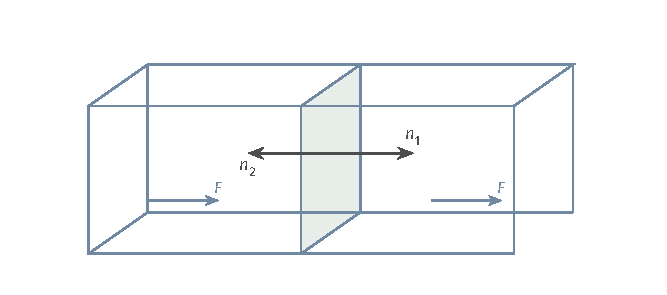
\includegraphics[width=112mm]{figures/01-mathematical-preliminaries-upper/01-mathematical-language-combinatorics-analysis-optimization/tikz/chapter3-concept-processes/gauss-shared-face.pdf}
 \caption{两个相邻单位立方体共用绿色面，图用斜投影表示三维几何。取常场$F=(1,0,0)^\top$，共同面上两侧外法向为$n_1=(1,0,0)^\top$与$n_2=-n_1$，对应通量为$1,-1$，相加抵消。整体外向净通量也为零，与散度为零一致；一般区域的散度定理仍需要前述条件与证明。}
 \label{fig:analysis-process-gauss-shared-face}
\end{figure}

例如半径$R>0$的球面取外法向，令$\bm F(\bm x)=\bm x/R$。球面上$\bm F=\bm n$，故通量也等于球面积。
由于$\operatorname{div}\bm F=3/R$，散度定理给出
\[
 \int_{\partial B_R}\bm F^\top\bm n\,\mathrm dS
 =\frac3R\operatorname{vol}(B_R)
 =\frac3R\frac{4\pi R^3}3=4\pi R^2.
\]
这里的球体积可由圆盘截面积分得到，结果与前面直接参数化球面求面积一致。

\subsubsection{多元分部积分}

一元分部积分把一个因子的导数转给另一个因子，并留下端点项。
在多元情形中，对乘积向量场使用散度公式，就得到相应的边界通量项。
\begin{theorem}[多元分部积分]
\label{thm:multivariable-integration-by-parts}
设$\Omega\subseteq\mathbb R^3$满足上述Gauss公式的区域条件。
若标量函数$u$在$\overline\Omega$的开邻域内连续可微，$v$在同一邻域内二阶连续可微，则
\[
 \int_\Omega u\Delta v\,\mathrm d\bm x
 =\int_{\partial\Omega}u\nabla v^\top\bm n\,\mathrm dS
  -\int_\Omega\nabla u^\top\nabla v\,\mathrm d\bm x.
\]
\end{theorem}
\begin{proof}
向量场$\bm F=u\nabla v$连续可微，逐坐标的乘积法则给出
\[
 \operatorname{div}(u\nabla v)
 =\nabla u^\top\nabla v+u\Delta v.
\]
将它代入Gauss公式，再把第一项的区域积分移到等式另一侧，即得结论。
\end{proof}
对满足Green公式条件的平面区域，同样的证明使用平面通量公式即可成立，边界面积元素相应换成弧长元素。
这一公式把$v$的二阶导数转移为$u$与$v$的一阶导数，同时保留法向边界项；该项是否为零，必须由具体边界条件决定。

\subsection{曲面积分与边界路径积分}

Gauss公式要求闭曲面围成空间区域。另一类问题只给一张有边界的定向曲面，要求比较曲面上的旋转累计与边界环流。
这时应使用旋度在曲面法向上的分量，不需要先把曲面补成闭曲面。

\subsubsection{Stokes公式}

在$z=0$平面上取向上法向时，旋度的法向分量就是Green公式中的$Q_x-P_y$。
Stokes公式将这一关系推广到空间中的定向曲面，同时要求法向与边界方向相容。
\begin{theorem}[Stokes定理]
\label{thm:multivariable-stokes}
设$S\subseteq\mathbb R^3$为紧致、可定向的分片$C^2$曲面，边界由有限条分段$C^1$简单闭曲线组成。
各光滑曲面片选取连续且片间定向相容的单位法向$\bm n$，边界采用其诱导方向。
若向量场$\bm F$在$S$的开邻域内连续可微，则\term{Stokes公式}（Stokes' theorem）给出
\begin{equation}
 \oint_{\partial S}\bm F^\top\,\mathrm d\bm r
 =\int_S(\nabla\times\bm F)^\top\bm n\,\mathrm dS.
 \label{eq:multivariable-stokes}
\end{equation}
\end{theorem}
这里的“可定向”要求各曲面片能相容地选择法向，使公共边上的诱导方向相反；有折角的接缝处不要求存在唯一法向。
两侧都为标量：左侧是原向量场的边界环流，右侧是其旋度穿过曲面的通量。

在一张参数曲面片上，可以把公式归结为参数平面上的Green公式。
设$\bm r(u,v)$在规则参数域$D$的邻域内二阶连续可微、在内部正则且一一对应，并采用$\bm r_u\times\bm r_v$确定的定向。
还要求参数边界按诱导方向对应曲面片的边界，从而可以沿$\partial D$计算边界路径积分。
记
\[
 \begin{aligned}
 A(u,v)&=\bm F(\bm r(u,v))^\top\bm r_u(u,v),\\
 B(u,v)&=\bm F(\bm r(u,v))^\top\bm r_v(u,v).
 \end{aligned}
\]
边界路径的链式法则将左侧变成$\oint_{\partial D}A\,\mathrm du+B\,\mathrm dv$。
对$A,B$逐项求偏导，含$\bm r_{uv}$与$\bm r_{vu}$的项因混合偏导相等而相消，剩下
\[
 \partial_uB-\partial_vA
 =\bigl(\operatorname{curl}\bm F\bigr)(\bm r(u,v))^\top
   (\bm r_u\times\bm r_v).
\]
参数平面上的Green公式因此给出该曲面片上的Stokes公式。
对有限张相容定向的曲面片，公共边的路径积分相消，只剩整张曲面的边界。
一般分片曲面的完整论证还需核对曲面覆盖及接缝条件，以上推导说明参数片上的机制；一般定理可参考所引教材\scite{math-strang1991calculus}。

\subsubsection{跨接曲面的选择}

Stokes公式的边界积分只由有向边界和边界上的向量场决定。因此，若两张满足定理条件的定向曲面具有同一有向边界，
且$\bm F$在两张曲面附近都连续可微，则两张曲面上的旋度通量相等。
计算时可以选较简单的跨接曲面，但必须核对向量场定义域，不能让替换曲面穿过场的奇点。

例如$\bm F=(-y/2,x/2,0)^\top$有$\nabla\times\bm F=(0,0,1)^\top$。
单位圆采用从上方看逆时针的方向，取向上单位圆盘$S$，便有
\[
 \oint_{\partial S}\bm F^\top\,\mathrm d\bm r
 =\iint_S1\,\mathrm dS=\pi.
\]
上半球面取外法向时，边界诱导方向相同，旋度通量仍为$\pi$。
若改用向下定向的圆盘，边界方向也必须反转，两个积分同时变号。


图~\ref{fig:analysis-process-stokes-spanning-surfaces}比较同一有向圆周的两张跨接曲面。替换曲面时，边界方向与场的定义域都要同时保留。
\begin{figure*}[!htbp]
 \centering
 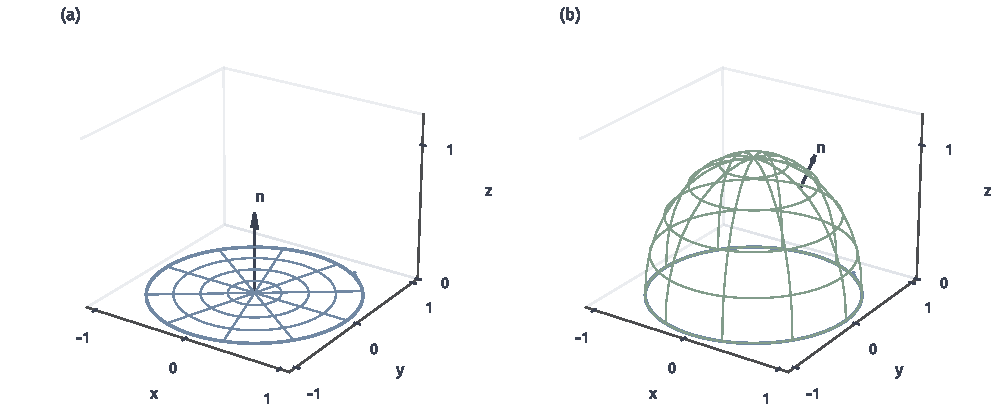
\includegraphics[width=169.0mm]{figures/01-mathematical-preliminaries-upper/01-mathematical-language-combinatorics-analysis-optimization/matplotlib/chapter3-concept-processes/stokes-spanning-surfaces.pdf}
 \caption{(a) 向上单位圆盘；(b) 外向上半单位球面。蓝色边界均从上方看逆时针，黑箭头标记各自法向。对$F=(-y/2,x/2,0)^\top$，旋度恒为$(0,0,1)^\top$，两面上的旋度通量都为$\pi$。右面面积为$2\pi$而非$\pi$；相等的是法向分量的累计，不能把通量当成面积。}
 \label{fig:analysis-process-stokes-spanning-surfaces}
\end{figure*}

\subsection{积分公式的比较}

前面的公式回答的都是导数在内部的积分与边界积分之间的关系，但内部对象、边界对象和方向条件各有不同。
一元基本定理以区间两端为边界；梯度场的路径积分基本定理以路径两端为边界。这里进一步得到下面三种关系。
\begin{center}
\begin{tabular}{lll}
\toprule
公式 & 内部积分 & 边界积分\\
\midrule
Green环流形式 & 平面区域的$Q_x-P_y$ & 正向路径的切向积分\\
Gauss & 空间区域的散度 & 闭曲面的外向通量\\
Stokes & 定向曲面的旋度通量 & 诱导方向的路径环流\\
\bottomrule
\end{tabular}
\end{center}
对向上定向的平面曲面，Stokes公式还原Green公式的环流形式；
Green公式的通量形式则是二维的散度公式。
普通标量函数的区域积分不自动具有边界表达：要使用这些公式，须先找到满足条件的向量场，使其散度或旋度的相应分量等于被积函数。

各公式均使用勒贝格积分。连续可微性、分片规则边界与定向是这里的经典公式所需的条件，并不是另换一种积分定义。
尤其要核对向量场是否在整个积分对象附近都有定义：前面穿孔平面上的场在原点无定义，就不能把包含原点的圆盘直接代入Green公式。
仅知道两个函数在体积测度下几乎处处相等，也不足以确定其边界积分，因为边界本身可以是体积零测集。
如果要降低导数或边界的规则性，还须另外建立弱导数、边界迹及相应的积分公式；不能沿用当前公式而省去这些条件。

\FloatBarrier


\FloatBarrier
\section{本章小结}
\label{sec:multivariable-summary}

多元可微性要求所有小扰动共享同一个线性映射，仅有坐标切片或各个固定方向的信息还不够。
区域、路径与曲面累计分别使用体积、弧长和曲面面积，有向路径与通量还保留方向。
Tonelli与Fubini定理控制逐坐标累计，Jacobian校正坐标变换的体积。
Green、Gauss和Stokes公式把特定导数的内部累计联系到边界，扩展一元微积分基本定理，
也各自要求明确的正则性、可积性和定向条件。

\chapter{最优化}
\label{chap:optimization}

第~\ref{chap:univariate-calculus}章和第~\ref{chap:multivariate-calculus}章给出了函数的局部变化和极限条件。若任务要求从所有允许参数中选出目标值最小的一个，局部变化能提供怎样的求解信息，计算出的候选又凭什么算作足够好？本章用带正则项的最小二乘与资源约束追踪这两个问题。设训练样本有$n\geq1$个，参数为$\bm w\in\mathbb R^d$，观测值组成$\bm y=(y_1,\ldots,y_n)^\top\in\mathbb R^n$，矩阵$\bm X$的第$i$行为预测输入$\bm x_i^\top$。拟合目标为
\begin{equation}
  F(\bm{w})
  =
  \frac{1}{2n}\lVert \bm{X}\bm{w}-\bm{y}\rVert_2^2
  +\frac{\lambda}{2}\lVert\bm{w}\rVert_2^2,
  \qquad
  \bm{X}\in\mathbb{R}^{n\times d},\quad \lambda\geq 0,
  \label{eq:opt-regularized-least-squares}
  % 保留内容迁移前的语义标签，指向同一公式。
\begingroup
\makeatletter
\let\label\ltx@label
\label{eq:prelim-regularized-least-squares}
\endgroup
\end{equation}
以及线性资源约束
\begin{equation}
  \bm{A}\bm{w}=\bm{b},\qquad
  \bm{G}\bm{w}\leq\bm{h}.
  \label{eq:opt-linear-resource-constraints}
\end{equation}
式~\eqref{eq:opt-regularized-least-squares}中的第一项汇总预测与观测之间的平方误差。正则项限制参数
规模，约束则直接排除超出预算的候选；两者看似都在“限制模型”，却改变了不同的数学对象。

同一个目标值误差可以由不同方法取得，但方法需要的信息与计算成本不同。光滑目标允许用梯度和曲率构造方向，非光滑项可能需要保留在可解子问题中，约束则要求同时核验候选的可行性。预算有限时，还可以改变每步读取的信息、变量范围或子问题精度；多个评价目标则需要另行规定怎样选择答案。这些条件可以同时出现，本章按“先确认问题有解，再选择利用什么信息”的顺序展开：第~\ref{sec:opt-objectives-solutions-curvature}节只回答最优解是什么、何时存在、局部信息能推出多少全局结论，不涉及具体算法；其后各节才按可用信息分类选择求解方法。为了固定比较口径，除拟合与资源两个例子之外，本章还使用以下二次目标
\begin{equation}
 f(\bm w)=\frac12(w_1^2+16w_2^2),\qquad
 \bm H=\operatorname{diag}(1,16),\qquad
 \bm w^{(0)}=(2,2)^\top.
 \label{eq:opt-common-quadratic}
\end{equation}
其最小点为零、初始目标值为$34$；两方向曲率的差异使方向、步长和每步成本都能直接核算。

后面的残差例子还将改变三项不同条件：非线性使线性化只在局部可靠，需要用实际下降决定是否接受阻尼步；少量偏大读数要求重新规定残差代价，可在MM上界下形成迭代权重；离散前向则可能没有有用的经典导数，指定的替代反向必须另外核验。它们分别改变步长控制、目标函数与反向规则，不能混作同一种正则化。

\section{优化问题的定义与基本性质}
\label{sec:opt-objectives-solutions-curvature}

目标有下界并不保证最优值能够达到，梯度为零也不保证候选已经最优。求解之前，需要分别建立解的含义、最优值达到的条件，以及局部比较能够推出哪些全局结论。存在性使用极限与可行域性质，凸性和曲率条件则连接局部信息、解的唯一性与误差界。后面的算法将各自调用这些保证。

\subsection{优化问题与解}
\label{sec:opt-problem-and-solutions}
\label{sec:opt-error-objects}

把实际问题写成优化问题，要做的是四项约定：哪些量可以调整（变量），允许取值到什么范围（可行域），按什么准则比较两个候选（目标函数），以及是否要求达到最优还是只需足够好。
这一步看似只是套格式，实际上回答的是“机器到底被允许做什么、按什么打分”：训练模型时
变量可以是模型参数，可行域是满足预算或非负约束的参数集合，比较候选则用目标函数，
例如样本损失的平均值与正则项之和。同一个任务若改变这些约定中的任何一项，
求出来的就可能是另一个决策。四项里任何一项写得不同，得到的答案就可能不同。例如同样想“让误差小”，若可行域写成整个空间，最优参数可能无界；若写成某个有界集合，答案就落在集合内；若比较准则改成绝对误差而不是平方误差，最优点也可能移动。因此优化问题的完整写法是

一个优化问题必须同时给出目标函数、变量和可行域。记
\[
  \min_{\bm{w}\in C}F(\bm{w}),\qquad
  C=\{\bm{w}\in\mathbb{R}^d:
  \bm{A}\bm{w}=\bm{b},\ \bm{G}\bm{w}\leq\bm{h}\}.
\]
变量$\bm w$是待选择的参数，目标$F$规定怎样比较候选，可行域$C$规定哪些候选允许采用。
若等式有$m$条、不等式有$p$条，则
$\bm A\in\mathbb R^{m\times d}$、$\bm b\in\mathbb R^m$、
$\bm G\in\mathbb R^{p\times d}$、$\bm h\in\mathbb R^p$，向量不等式逐坐标理解。
若$C=\varnothing$，问题\term{不可行}（infeasible）；若$C\neq\varnothing$但
$\inf_{\bm{w}\in C}F(\bm{w})=-\infty$，问题\term{无下界}（unbounded below）。
只有可行且有有限下界，才值得继续问下确界是否由某个点达到。
例如同时要求$x\leq0$和$x\geq1$就不可行；
在实线上最小化$x$无下界，$\inf_{x\in\mathbb R}e^x=0$有下界却没有最小点；
把$x$限制在$[0,1]$后，后一问题的最小值变为$1$且在$0$达到。
最优值是数$F^\star=\inf_C F$，最优解集合是$\argmin_C F$，后者可以为空或包含多个点。
写出问题$\min_C F$表示求最小值的任务，并不代替存在性证明；
声称某个数等于$\min_C F$时，才需要确认它确实被可行点取得。可行的判别方式是分开报告
两件事：最优值是多少，以及是否有可行点达到它。例如$\min_{w\in[0,1]}w$的最优值$0$
由$w=0$取得；$\min_{w>0}w$的最优值仍为$0$，却没有点取得，因为可行域不含$0$。
两种情形下最优值相同，可用的结论完全不同。

\begin{definition}[全局解、局部解与无约束驻点]
\label{def:opt-solutions-stationarity}
设$C\subseteq\mathbb R^d$非空，$F:C\to\mathbb R$。\term{全局最优解}（global minimizer）$\bm{w}^{\star}\in C$满足
$F(\bm{w}^{\star})\leq F(\bm{w})$对所有$\bm{w}\in C$成立。\term{局部最优解}
（local minimizer）要求存在$r>0$，使该不等式对所有
$\bm w\in C\cap B(\bm w^\star,r)$成立。
无约束可微问题的\term{驻点}（stationary point）满足
$\nabla F(\bm{w})=\bm{0}$。驻点只是局部一阶变化消失，可能是极小点、极大点或
第~\ref{sec:multivariable-curvature-error}节所说的微分鞍点。
\end{definition}
给定$\varepsilon>0$和可行候选$\widehat{\bm w}\in C$，若
\[
  F(\widehat{\bm{w}})-\inf_{\bm{w}\in C}F(\bm{w})\leq\varepsilon,
\]
就称$\widehat{\bm{w}}$为目标值意义下的$\varepsilon$近似解。对无约束可微问题，
另一种常见标准是
$\lVert\nabla F(\widehat{\bm{w}})\rVert_2\leq\varepsilon$；在没有额外曲率条件时，
这两种近似不能互换。一般约束问题的精确最优点也可能有非零梯度；
后面的约束求解将建立同时反映允许移动方向与可行性的停止标准。

只报一个停止量而不说明它衡量什么，会掩盖实际精度。小梯度说明当前点附近已经没有
值得利用的一阶方向，却不说明离最优值还有多远；小目标差说明接近最优值，却不说明参数
是否唯一；参数距离小则依赖参照解的选择。三种量在不同的曲率条件下互相控制，下面先看
它们在一维的分化。取
$f(x)=\epsilon x^2/2$、$\epsilon=10^{-8}$；在$x=10^6$处，
梯度只有$0.01$，目标值却比最小值高$5000$，到最小点$0$的距离仍为$10^6$。
平坦方向把一阶变化压得很小，因此梯度停止标准首先回答的是局部变化是否足够小。
把小梯度换成小目标差，还需要梯度与目标差之间的定量条件；
把目标差换成参数距离，又需要相应的曲率下界。后文将分别建立这些界，
使用时必须同时带上它们的常数。

前面的目标值近似标准只比较目标与最优值之间的差距。评价同一个近似参数时，还可以关心它离某个参照参数多远，
或者它的预测发生了多大变化。这三个问题要分别选择误差对象。
下面暂取$C=\mathbb{R}^d$，不加资源约束，以式~\eqref{eq:opt-regularized-least-squares}为目标。
令$F^\star=\inf_{\bm{w}\in\mathbb{R}^d}F(\bm{w})$；若选定一个最小点
$\bm{w}^\star$，则
\[
  F(\widehat{\bm{w}})-F^\star,\qquad
  \lVert\widehat{\bm{w}}-\bm{w}^\star\rVert_2,\qquad
  \left(
    \frac{1}{n}\sum_{i=1}^{n}
    \bigl(
      \widehat{\bm{w}}^{\top}\bm{x}_i
      -(\bm{w}^\star)^{\top}\bm{x}_i
    \bigr)^2
  \right)^{1/2}
\]
分别是目标值误差、参数误差和在给定样本输入上的预测误差。最小点不唯一时，参数误差还
需要指定参照解，或改成到最小点集合的距离。三种误差衡量不同对象，彼此能否控制取决于
目标曲率、数据矩阵和参数化；一个误差较小不能无条件推出另两个也较小。

例如，在$n=1$、$\bm{x}_1=(1,0)^\top$、$y_1=0$、$\lambda=0$时，
目标函数为$F(w_1,w_2)=w_1^2/2$。参照解$(0,0)$与参数$(0,100)$的目标值都为$0$，
在这个样本输入上的预测也相同，参数距离却是$100$。差别来自目标和当前观测都没有约束
第二个坐标；并不是把目标误差算得更精确就能补回这项信息。

若希望在一个目标式中同时比较代价并排除不可行点，可以约定不可行点的代价为$+\infty$。
这种扩展实值表达把约束并入函数，后面的非光滑子问题就不必另写一套可行域符号。
\begin{definition}[适当函数、有效定义域与约束指标]
\label{def:opt-proper-domain-indicator}
函数$f:\mathbb R^d\to\mathbb R\cup\{+\infty\}$若不恒为$+\infty$，称为适当函数；
它从不取$-\infty$。其\term{有效定义域}（effective domain）为
$\operatorname{dom}f=\{\bm x:f(\bm x)<+\infty\}$。
集合$C$的扩展实值指标函数为$\iota_C(\bm x)=0$（$\bm x\in C$），在其余点取$+\infty$。
\end{definition}
它不同于前文计数与分析中使用的指示函数$\mathbb I\{\cdot\}$：后者在条件成立时取$1$、
否则取$0$，只给集合成员作标记；$\iota_C$在$C$外取$+\infty$，把不允许的点排除出最小化。
于是$\min_{\bm w\in C}F(\bm w)$可统一写成
$\min_{\bm w\in\mathbb R^d}\{F(\bm w)+\iota_C(\bm w)\}$。
有限惩罚只是不喜欢违规候选，$+\infty$才真正将它排除。有效定义域记录有有限代价的点，
适当性保证至少还有一个这样的点；它不保证有下界、更不保证最小值达到。

\subsection{最优解的存在}
\label{sec:opt-existence}

在讨论怎样求解之前，必须先确认所要找的对象存在。一个下确界可能由可行点达到，也可能只是逼近而达不到；若连最优点都不存在，任何算法返回的候选都不可能是它。判断存在性的通用做法甚至不需要算法：即使暂时不知道如何求解，也能选择一列目标值越来越接近下确界的候选，称为最小化序列。
有限下确界$m$时，可逐项选取$F(\bm w^{(k)})\leq m+1/k$；若下确界为$-\infty$，
则可逐项要求$F(\bm w^{(k)})\leq-k$。要从这些候选得到最优点，须回答三个问题：
序列能否取到收敛子列，极限是否仍可行，目标值比较能否传到极限。
若$C\subseteq\mathbb{R}^d$非空且紧，$F:C\to\mathbb{R}$连续，则
定理~\ref{thm:multivariable-extreme-value}保证$F$在$C$上达到全局最小值。这里直接复用
第~\ref{chap:multivariate-calculus}章的极值存在结论。

可行域不紧时，目标本身也可能阻止最小化序列逃向无穷远。
\begin{definition}[强制性与下半连续性]
\label{def:opt-coercive-lower-semicontinuous}
设$C\subseteq\mathbb R^d$，$F:C\to(-\infty,+\infty]$。若沿$C$中的任意序列，
$\lVert\bm{w}\rVert_2\to\infty$时$F(\bm{w})\to\infty$，称$F$是
\term{强制的}（coercive）。$F$在$C$上\term{下半连续}
（lower semicontinuous）要求对每个收敛序列
$\bm{w}^{(k)}\to\bm{w}$都有
\[
  F(\bm{w})\leq\liminf_{k\to\infty}F(\bm{w}^{(k)}).
\]
其中序列与极限点均属于$C$。
\end{definition}
连续性并不是存在性证明所需的最弱条件。下半连续性允许函数值在极限点向下跳，
却不允许极限点的函数值突然高于邻近值。等价地，每个
下水平集$\{\bm{w}\in C:F(\bm{w})\leq a\}$在$C$的相对拓扑中都是闭集。

设$C$非空且闭，$F:C\to(-\infty,+\infty]$下半连续、强制，并且不恒为
$+\infty$且从不取$-\infty$。取$\bar{\bm{w}}\in C$使
$F(\bar{\bm{w}})<+\infty$，再把最小化序列限制到下水平集
\[
  K=\{\bm{w}\in C:F(\bm{w})\leq F(\bar{\bm{w}})\}.
\]
若$\inf_C F=F(\bar{\bm{w}})$，则$\bar{\bm{w}}$已经是最小点；否则
$\inf_C F<F(\bar{\bm{w}})$，任一最小化序列从某项起都落入$K$，可以只保留这段尾序列。
强制性使$K$有界，下半连续性与$C$的闭性使$K$闭，故$K$在有限维空间中紧。该尾序列
有子列收敛到$\bm{w}^{\star}\in K$，而下半连续性给出
$F(\bm{w}^{\star})\leq\liminf_kF(\bm{w}^{(k)})=\inf_C F$。因此下确界达到。
若原先假设下确界为$-\infty$，同一不等式会迫使$F(\bm w^\star)=-\infty$，
与适当性矛盾；所以这些条件也排除了无下界情形。
这个证明也指出各条件的职责：强制性阻止序列逃向无穷远，闭性保留可行极限，下半连续性
把目标值比较传到极限点。
当$\lambda>0$时，式~\eqref{eq:opt-regularized-least-squares}满足
$F(\bm{w})\geq\lambda\lVert\bm{w}\rVert_2^2/2$，所以即使可行域无界也不会沿参数
无穷大的方向降低目标。这里的推理顺序是：先用下界排除无下界情形，再用强制性得到有界的
下水平集，最后由闭性和下半连续性把极限留在可行域内。三项目标各自对应一个条件，
缺少任何一项都可能让最小化序列逃向无穷远或边界。


图~\ref{fig:vol1-add-coercive-sublevels}把“留在有界区域”与“逃向无穷远”分开。$x^2$的有限下水平集有界，$e^{-x}$却可以通过让$x$持续增大来逼近达不到的下确界。
\begin{figure}[!htb]
  \centering
  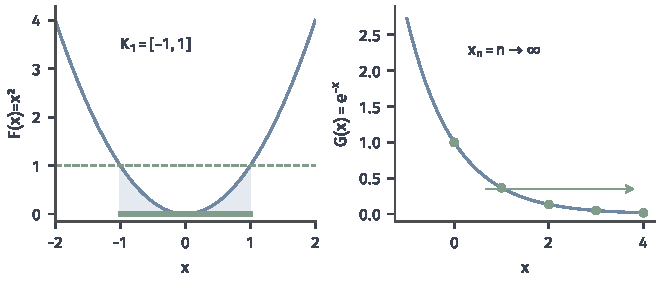
\includegraphics[width=112mm]{figures/01-mathematical-preliminaries-upper/01-mathematical-language-combinatorics-analysis-optimization/matplotlib/comprehension-additions/coercive-sublevels.pdf}
  \caption{全实线上的两个连续目标。左图$F(x)=x^2$的下水平集$K_1=\{x:F(x)\leq1\}=[-1,1]$有界；右图$G(x)=e^{-x}$沿$x_n=n$趋近下确界$0$，但没有最小点。左侧浅色仅标出下水平范围内的函数图下区域，绿线才表示参数集合$K_1$。这组例子说明存在性条件的职责，不声称强制性是任何最小点存在的必要条件。}
  \label{fig:vol1-add-coercive-sublevels}
\end{figure}

\noindent\begin{minipage}{\linewidth}
\subsection{凸性条件下的最优解性质}
\label{sec:opt-convexity}

\subsubsection{凸性与全局最优}

局部最优只比较附近候选；要把这项保证扩展到全部可行域，需要让远处更优的候选也能影响附近的比较。
为什么普通函数做不到这一点？设想目标里有两个互相隔开的山谷，站在其中一个谷底向四周看
都更高，局部上它已经最优，但另一处山谷可能更低；局部信息里完全没有远处山谷的线索。
若任意两个可行点之间的线段都可行，而且沿线段的目标值不超过两端值的加权平均，那么只要
远处有一个更低的点，连向它的整条线段都不能高于两端连线，当前点附近就一定存在更低的点，
从而排除“假谷底”。这两项条件分别是集合与函数的凸性。
\end{minipage}\par
\begin{definition}[凸集与凸函数]
\label{def:opt-convex-set-function}
集合$C\subseteq\mathbb R^d$为\term{凸集}（convex set），是指对任意
$\bm{u},\bm{v}\in C$和$\theta\in[0,1]$，
$\theta\bm{u}+(1-\theta)\bm{v}\in C$。线性等式、线性不等式和范数球的解集都是凸集，
它们的交集仍为凸集，所以式~\eqref{eq:opt-linear-resource-constraints}定义凸可行域。

定义在凸集$C$上的函数$f:C\to\mathbb R$若对任意$\bm u,\bm v\in C$和$\theta\in[0,1]$满足
\begin{equation}
  f(\theta\bm{u}+(1-\theta)\bm{v})
  \leq
  \theta f(\bm{u})+(1-\theta)f(\bm{v}),
  \label{eq:opt-convex-function}
\end{equation}
就称为\term{凸函数}（convex function）。若$-f$凸，则称$f$凹。
\end{definition}
式右侧的$\theta f(\bm u)+(1-\theta)f(\bm v)$是两个函数值的\term{加权平均}（weighted average）：
两个非负系数之和为$1$，分别规定两个值在平均中所占的份额。
凸函数的函数图像位于任意弦段下方。若远处存在更小的函数值，连向该点的线段就会在当前点附近给出更小的值\scite{math-boyd2004convex}

\begin{theorem}[凸函数的一阶与二阶判据]
\label{thm:opt-convexity-criteria}
设$C$为开凸集。可微函数$f:C\to\mathbb{R}$凸，当且仅当对任意
$\bm{u},\bm{v}\in C$，
\begin{equation}
  f(\bm{v})\geq f(\bm{u})
  +\langle\nabla f(\bm{u}),\bm{v}-\bm{u}\rangle.
  \label{eq:opt-first-order-convexity}
\end{equation}
若$f$二阶可微，则这又等价于
$\nabla^2f(\bm{w})\succeq\bm{0}$对所有$\bm{w}\in C$成立。
\end{theorem}

\begin{proof}
若$f$凸，令$\phi(t)=f(\bm{u}+t(\bm{v}-\bm{u}))$。由凸性，
$[\phi(t)-\phi(0)]/t\leq\phi(1)-\phi(0)$。令$t\downarrow0$便得
式~\eqref{eq:opt-first-order-convexity}。反过来，令
$\bm{z}=\theta\bm{u}+(1-\theta)\bm{v}$，分别把一阶不等式用于
$(\bm{z},\bm{u})$和$(\bm{z},\bm{v})$，乘以$\theta$与$1-\theta$后相加，
线性项抵消，得到式~\eqref{eq:opt-convex-function}。

若$f$凸，把一阶判据用于$\bm{w}$与$\bm{w}+t\bm{v}$，再对$t$求二阶局部极限，
得到$\bm{v}^{\top}\nabla^2f(\bm{w})\bm{v}\geq0$。反之，沿任意线段定义
$\phi(t)$，则
$\phi''(t)=(\bm{v}-\bm{u})^{\top}\nabla^2f(\bm{u}+t(\bm{v}-\bm{u}))
(\bm{v}-\bm{u})\geq0$，一元函数$\phi$凸，故$f$凸。
\end{proof}

反复应用二点凸性可得\term{Jensen不等式}（Jensen's inequality）。若
$\alpha_i\geq0$且$\sum_i\alpha_i=1$，则
\begin{equation}
  f\left(\sum_{i=1}^m\alpha_i\bm{w}_i\right)
  \leq\sum_{i=1}^m\alpha_i f(\bm{w}_i).
  \label{eq:opt-jensen}
\end{equation}
归纳步骤把前$m-1$个点先归一化为一个加权平均，再与第$m$个点应用二点凸性。
具体地，若$\alpha_m<1$，取
$\bm z=\sum_{i<m}\alpha_i\bm w_i/(1-\alpha_m)$，归纳假设给
$f(\bm z)\leq\sum_{i<m}\alpha_i f(\bm w_i)/(1-\alpha_m)$；
再用于$(1-\alpha_m)\bm z+\alpha_m\bm w_m$即可。若$\alpha_m=1$，结论直接为等式。
这个证明也说明非负和归一化不是装饰条件；允许负权重后，组合点可能落到凸包之外，
因而不能再由凸性保证Jensen不等式。

凸性还把最优性变成可核验的一阶条件。若$f$可微且凸，则
$\nabla f(\bm{w}^{\star})=\bm{0}$代入式~\eqref{eq:opt-first-order-convexity}
便得$f(\bm{v})\geq f(\bm{w}^{\star})$，因此凸问题的驻点是全局最小点。反过来，
非凸问题即使找到驻点，也只能说明该点附近没有一阶下降方向。
凸集$C$上凸函数的每个局部最小点都是全局最小点，且不要求可微：
若$\bm u$局部最优而某个$\bm v\in C$满足$f(\bm v)<f(\bm u)$，则对任意$t\in(0,1)$，
$\bm u+t(\bm v-\bm u)\in C$且
$f(\bm u+t(\bm v-\bm u))\leq(1-t)f(\bm u)+tf(\bm v)<f(\bm u)$。
取足够小的$t$便与局部最优矛盾。对于边界上的约束最优点，仍不能反推普通梯度为零。
图~\ref{fig:opt-convex-chord-tangent}同时画出这两侧的界。弦在图像上方，源于二点凸组合；
切线在图像下方，源于可微凸函数的一阶判据。二者夹住函数，却来自不同的比较对象，
不能把某点处的切线误当作连接两个函数值的弦。
\begin{figure}[htbp]
  \centering
  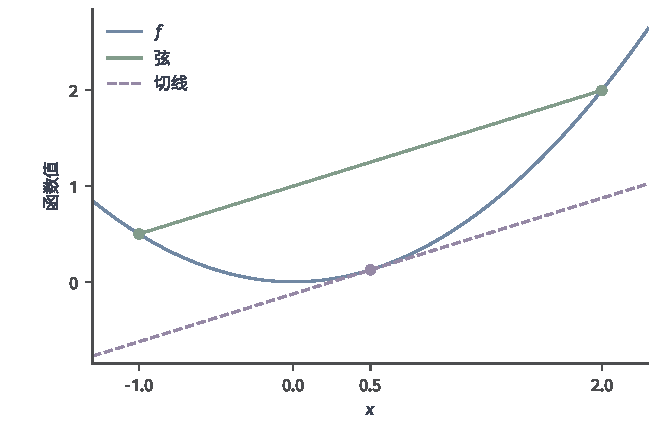
\includegraphics[width=112.0mm]{figures/01-mathematical-preliminaries-upper/01-mathematical-language-combinatorics-analysis-optimization/matplotlib/opt-convex-chord-tangent/figure.pdf}
  \caption{$f(x)=x^2/2$的弦与切线。蓝线为函数，绿线连接$u=-1$与$v=2$的函数值，
 在这两个输入之间给出弦上界；紫虚线是在$x_0=1/2$处的一阶仿射下界，适用于整个实线。
 绿线的上界只在其端点之间使用，切线下界来自凸性。图为解析教学示例。}
 \label{fig:opt-convex-chord-tangent}
\end{figure}

对扩展实值目标，式~\eqref{eq:opt-convex-function}在有限取值的点上检验，
并要求有效定义域凸；这避免在端点权重为零时操作$0\cdot(+\infty)$。

\subsubsection{严格凸性与解的唯一性}

凸函数可以沿某个方向保持不变，局部到全局的保证并没有排除多个最小点。
最小点不唯一会影响两件事：返回哪一个解取决于算法细节而不是问题本身，与最小点距离
有关的误差界也无从定义。若希望排除这种平坦的最优线段，需要把不同点之间的凸性不等式
加强为严格不等式。
\begin{definition}[严格凸函数]
\label{def:opt-strict-convexity}
设$C$凸，$f:C\to\mathbb R$。若式~\eqref{eq:opt-convex-function}对所有
$\bm u\neq\bm v$及$0<\theta<1$严格成立，则称$f$严格凸。
\end{definition}
若两个不同点$\bm u,\bm v$都达到最小值$m$，严格凸性使其中点的函数值严格小于
$(m+m)/2=m$，矛盾。因此它只保证至多一个最小点；严格凸函数$e^x$在实线上仍没有最小点。
存在性必须另由前一小节的条件检验。
在式~\eqref{eq:opt-regularized-least-squares}中，$\lambda=0$且$\bm X$不满列秩时沿零空间
方向目标不变；$\bm X$满列秩或$\lambda>0$时，任意非零方向$\bm d$都有
$\|\bm X\bm d\|_2^2/n+\lambda\|\bm d\|_2^2>0$，故目标严格凸。
与闭可行域上的存在性合用，才能断言有唯一解。

\subsubsection{强凸性与误差控制}

严格凸保证最小点至多一个，却不给统一曲率下界：两个严格凸函数可以一个像浅口碗、一个像
深漏斗，而严格凸的定义只要求“中点严格更低”，没有规定低多少。这个“低多少”直接决定
从目标误差能换回多小的参数误差，也决定梯度类算法收敛得快慢。强凸性则要求弦段与函数之间至少留出一个与距离平方成比例的间隔。
这个定义可以用于非光滑正则项，也可以使用欧氏范数以外的范数。

\begin{definition}[相对于范数的强凸性]
\label{def:opt-strong-convexity}
设$C$是实赋范空间中的凸集，$f:C\to\mathbb{R}$，$\mu>0$。若对任意
$\bm{u},\bm{v}\in C$和$\theta\in[0,1]$都有
\begin{equation}
 f(\theta\bm{u}+(1-\theta)\bm{v})
 \leq\theta f(\bm{u})+(1-\theta)f(\bm{v})
 -\frac{\mu}{2}\theta(1-\theta)\lVert\bm{u}-\bm{v}\rVert^2,
 \label{eq:opt-norm-strong-convexity}
\end{equation}
则称$f$相对于$\lVert\cdot\rVert$是\term{$\mu$强凸}（$\mu$-strongly convex）的。
\end{definition}

在欧氏空间的开凸集上，若$f$可微，强凸性等价于一阶下界
\begin{equation}
  f(\bm{v})\geq f(\bm{u})+
  \langle\nabla f(\bm{u}),\bm{v}-\bm{u}\rangle
  +\frac{\mu}{2}\lVert\bm{v}-\bm{u}\rVert_2^2.
  \label{eq:opt-first-order-strong-convexity}
\end{equation}
可用定理~\ref{thm:opt-convexity-criteria}对
$f(\bm{w})-\mu\lVert\bm{w}\rVert_2^2/2$应用凸性判据得到这一等价关系；若$f$二阶可微，
它又等价于$\nabla^2f(\bm{w})\succeq\mu\bm{I}$。一般范数的平方未必是欧氏二次型，
因此不能把这一Hessian写法直接当作所有范数下的定义。
例如$|x|+\mu x^2/2$虽在$0$处不可微，仍相对于绝对值范数$\mu$强凸：绝对值部分满足
凸性，二次部分恰好提供式~\eqref{eq:opt-norm-strong-convexity}中的距离平方间隔。

强凸性还能把目标差转成参数距离。设$f$在凸集$C$上$\mu$强凸，且最小点$\bm w^\star$存在。
把定义用于$\bm w^\star$与任意$\bm w\in C$，并用最优性给线段上的函数值加下界，得到
\[
 f(\bm w^\star)\leq(1-t)f(\bm w^\star)+tf(\bm w)
 -\frac{\mu}{2}t(1-t)\|\bm w-\bm w^\star\|^2.
\]
除以$t>0$再令$t\downarrow0$，可得
\begin{equation}
 f(\bm w)-f(\bm w^\star)\geq\frac{\mu}{2}\|\bm w-\bm w^\star\|^2,
 \qquad
 \|\bm w-\bm w^\star\|\leq\sqrt{\frac{2(f(\bm w)-f^\star)}{\mu}}.
 \label{eq:opt-strong-convex-distance}
\end{equation}
证明并未假设最优点在内部，因此也适用于固定凸域上的非光滑目标。

抗扰动结论必须明确扰动对象。现在使用欧氏范数，固定同一个凸集$C$，只改变线性项：
$f_{\bm b}(\bm w)=f(\bm w)-\langle\bm b,\bm w\rangle$。
设$\bm w_{\bm b}$与$\bm w_{\bm c}$分别达到这两个强凸问题的最小值。
把式~\eqref{eq:opt-strong-convex-distance}分别用于两个目标后相加，得
\[
 \mu\|\bm w_{\bm b}-\bm w_{\bm c}\|_2^2
 \leq\langle\bm b-\bm c,\bm w_{\bm b}-\bm w_{\bm c}\rangle,
 \qquad
 \|\bm w_{\bm b}-\bm w_{\bm c}\|_2\leq\frac{\|\bm b-\bm c\|_2}{\mu}.
\]
这里没有改变可行域，也没有任意改变目标的曲率。约束边界变化造成的活跃集切换，
不能由这个线性扰动界一并处理。

式~\eqref{eq:opt-regularized-least-squares}的Hessian矩阵为
$\bm{X}^{\top}\bm{X}/n+\lambda\bm{I}$。当$\lambda>0$时，正则项把所有缺失曲率的
方向至少抬高到$\lambda$，因而目标$\lambda$强凸。若$\lambda=0$且$\bm{X}$不满列秩，
驻点仍是全局最优点，但解不唯一；若目标再加入非凸项，驻点甚至不再保证局部最小。

前述零空间退化满足$F(\bm w+t\bm v)=F(\bm w)$，说明曲率缺失可以产生多个解。
即使曲率处处为正且解唯一，数值问题也可能非常敏感。例如令$0<\epsilon\ll1$并考虑
\[
  f_b(w_1,w_2)=\frac12(\epsilon w_1^2+w_2^2)-bw_1.
\]
它对每个$b$都有唯一最小点$(b/\epsilon,0)$，但$b$改变$\Delta b$会使第一坐标改变
$\Delta b/\epsilon$。它是一般二次目标$\frac12\bm w^\top\bm H\bm w-\bm g^\top\bm w$在
$\bm H=\operatorname{diag}(\epsilon,1)$、$\bm g=(b,0)^\top$时的特例；拟合目标
式~\eqref{eq:opt-regularized-least-squares}去掉常数$\lVert\bm y\rVert_2^2/(2n)$后也有这种形式，其中
\[
  \bm{H}=\frac{1}{n}\bm{X}^{\top}\bm{X}+\lambda\bm{I},\qquad
  \bm g=\frac1n\bm X^\top\bm y.
\]
在对角例中，每个坐标方向都只被$\bm H$乘上一个曲率数。
对一般实对称$\bm H$，这里需要的结构结论是：可以选取$d$个单位正交方向
$\bm v_i$，使$\bm H\bm v_i=\lambda_i\bm v_i$，并使每个向量都能唯一写成
$\sum_i a_i\bm v_i$。这些方向和缩放数分别称为特征向量与特征值；
实对称矩阵的这种正交展开见定理~\ref{thm:ls-real-symmetric-spectral}。
若$\bm H\succ\bm0$，则
$\lambda_i=\bm v_i^\top\bm H\bm v_i>0$；记其中最小、最大者为
$\lambda_{\min}(\bm H)$、$\lambda_{\max}(\bm H)$。
展开涵盖全部方向，所以$\bm H^{-1}$在每个方向除以$\lambda_i$后，
任意向量的欧氏长度至多放大$1/\lambda_{\min}(\bm H)$倍。
当$\bm{H}\succ\bm{0}$时，最小点由$\bm H\bm w=\bm g$唯一确定；若线性项受到加性扰动
$\delta\bm{g}$，解的变化$\delta\bm w=\bm H^{-1}\delta\bm g$满足
\[
  \lVert\delta\bm{w}\rVert_2
  \leq
  \frac{1}{\lambda_{\min}(\bm{H})}
  \lVert\delta\bm{g}\rVert_2.
\]
因此$1/\lambda_{\min}(\bm{H})$控制固定尺度加性扰动的绝对放大；经过目标和变量尺度
归一化后，条件数
$\kappa(\bm{H})=\lambda_{\max}(\bm{H})/\lambda_{\min}(\bm{H})$
才刻画相对病态程度。例如$\bm{H}=\epsilon\bm{I}$的条件数为$1$，但绝对扰动仍会被
放大$1/\epsilon$倍。唯一性回答“解有几个”，敏感性还取决于所采用的扰动尺度，
不能只由唯一性或条件数笼统判断。

\section{无约束光滑目标的求解}
\label{sec:opt-smooth-iterative-methods}

有了可判定的最优性条件，还需构造能逐步接近它的参数序列。这里先限定目标可微且梯度光滑：
梯度下降用一阶信息保证单步改善，动量和预条件再利用迭代历史或曲率改变移动方向。
每种改进的保证都应与前节的曲率条件配对，而不能仅凭更新公式判断快慢。

这一节的所有更新都只在当前点附近使用局部信息，因此需要先回答两个问题：梯度给出的是
什么信息，以及顺着它走多远才安全。前一节的条件（光滑性、强凸性、PL）恰好为第二个问题
提供常数。各小节的差别就在于利用了哪一类信息：只有当前梯度、还利用历史方向，或者还
构造曲率矩阵。非线性残差的二阶分支还要比较模型预报与实际下降，由此决定接受候选及调整阻尼；拟牛顿分支则利用已走过的位移近似曲率，二者省略的信息不同。

\subsection{基于一阶信息的求解}
\label{sec:opt-first-order-methods}

一阶方法在当前候选附近计算线性变化，借此选择新的参数：梯度给出函数在该点最陡的
上升方向，以及沿每个方向的一阶变化率，但不给出这些变化率会怎样随位置改变。
一个直觉是，梯度只告诉你“站在山坡上，正前方哪边最陡”，却不告诉你坡势会在多远之后
变缓、转弯或出现另一个谷底；因此只凭梯度选方向，还必须另外决定迈多大一步。梯度下降
只用当前梯度；动量和加速还保留已有更新的信息，用来抵消陡峭方向上的来回摆动，并加快
平坦方向上的推进；两者都不要求显式构造Hessian。它们共用一阶信息，区别在于历史信息
怎样进入新的候选，以及这一点改变使步长允许取多大。

\subsubsection{基于梯度下降的求解}
\label{sec:opt-gradient-descent}

沿着负梯度走足够小的一步一定会下降：把位移写成$\bm d=-\eta\nabla f(\bm w)$并代入
一阶近似，函数值的变化约为$-\eta\lVert\nabla f(\bm w)\rVert_2^2$，是负的。
问题在于“足够小”没有一个可以事先使用的尺度：位移越大，被舍弃的高阶项影响越大，
下降保证可能失效。要把它换成可以计算的步长范围，需要控制移动后梯度会改变多少。
下面的光滑性条件为任意两点的梯度差提供统一上界。
可以用一个具体数字理解这条假设的作用：它给“每移动单位距离，梯度最多改变多少”定了一个
上限$L$，于是步长取$1/L$量级时，高阶项造成的反弹不会盖过一阶下降；没有这个$L$，
就无法给出一个任何位置都安全的固定步长。
\begin{definition}[欧氏梯度光滑性]
\label{def:opt-smoothness}
设$C\subseteq\mathbb R^d$开且凸，$f:C\to\mathbb R$可微，$L\geq0$有限。
$f$为\term{$L$光滑}（$L$-smooth），是指对任意$\bm u,\bm v\in C$，梯度满足
$\lVert\nabla f(\bm{u})-\nabla f(\bm{v})\rVert_2
\leq L\lVert\bm{u}-\bm{v}\rVert_2$。
\end{definition}
这里对梯度使用同一Lipschitz常数。强凸给下曲率，光滑给上曲率；$x^4$严格凸但
不在全实线上强凸，也不在全实线上具有有限的光滑常数。

梯度给出最陡的一阶下降方向：在一阶近似$f(\bm w)+\langle\nabla f(\bm w),\bm d\rangle$中，
要使增量最小，就应取$\bm d$与梯度方向相反，因为$\langle\nabla f,\bm d\rangle$
在固定$\lVert\bm d\rVert_2$时于$\bm d=-\lVert\bm d\rVert_2\nabla f/\lVert\nabla f\rVert_2$
取得最小值。但一步走多远取决于函数弯曲程度，一阶近似本身不能回答；光滑性把局部线性近似的
余项控制为二次量\scite{math-nocedal2006numerical}。本小节考虑可微函数
$f:\mathbb R^d\to\mathbb R$，并选取一个正的梯度Lipschitz上界$L>0$。
若梯度恒定，仍可选择任意正上界；这样后面的$1/L$步长也有定义。
全空间的设定保证更新点仍在函数定义域内；若目标只定义在开凸子域上，使用下降引理时
还须确认两端点及其线段留在该域内，不能直接把任意梯度步代入。

\begin{lemma}[下降引理]
\label{lem:opt-descent}
若$f:\mathbb R^d\to\mathbb R$可微且梯度是$L$-Lipschitz连续的，$L>0$，则对任意
$\bm u,\bm v\in\mathbb R^d$，
\begin{equation}
  f(\bm{v})\leq f(\bm{u})
  +\langle\nabla f(\bm{u}),\bm{v}-\bm{u}\rangle
  +\frac{L}{2}\lVert\bm{v}-\bm{u}\rVert_2^2.
  \label{eq:opt-descent-lemma}
\end{equation}
\end{lemma}

\begin{proof}
令$\bm{d}=\bm{v}-\bm{u}$。沿线段积分并减去一阶项可得
\[
  f(\bm{v})-f(\bm{u})-\langle\nabla f(\bm{u}),\bm{d}\rangle
  =
  \int_0^1
  \langle\nabla f(\bm{u}+t\bm{d})-\nabla f(\bm{u}),\bm{d}\rangle\,dt.
\]
由Cauchy--Schwarz不等式和梯度Lipschitz条件，被积函数至多为
$Lt\lVert\bm{d}\rVert_2^2$；积分即得结论。
\end{proof}

在当前点$\bm w$，一阶近似为$f(\bm w)+\langle\nabla f(\bm w),\bm d\rangle$。
给定步长$\eta>0$，给这条近似加上控制移动幅度的$\|\bm d\|_2^2/(2\eta)$，其唯一最小增量是
$\bm d=-\eta\nabla f(\bm w)$。由此得到梯度下降更新
\begin{equation}
  \bm{w}^{(t+1)}
  =\bm{w}^{(t)}-\eta\nabla f(\bm{w}^{(t)}).
  \label{eq:opt-gradient-descent}
\end{equation}
把更新后的点代入下降引理，得到
\begin{equation}
  f(\bm{w}^{(t+1)})
  \leq f(\bm{w}^{(t)})
  -\eta\left(1-\frac{L\eta}{2}\right)
  \lVert\nabla f(\bm{w}^{(t)})\rVert_2^2.
  \label{eq:opt-gradient-single-step}
\end{equation}
所以$0<\eta<2/L$保证每个非驻点处严格下降。若$f$下有界，记其有限下确界为
\[
  f_{\inf}:=\inf_{\bm{w}\in\mathbb{R}^d}f(\bm{w})>-\infty.
\]
取$\eta=1/L$并对$t=0,\ldots,T-1$求和，可得非凸光滑情形的保证
\begin{equation}
  \min_{0\leq t<T}\lVert\nabla f(\bm{w}^{(t)})\rVert_2^2
  \leq
  \frac{2L(f(\bm{w}^{(0)})-f_{\inf})}{T}.
  \label{eq:opt-nonconvex-gradient-rate}
\end{equation}
它只说明某次迭代接近驻点，没有声称驻点是全局最优点。

步长上界在一维二次函数上即可看到。对$f(w)=Lw^2/2$，
$w^{(t+1)}=(1-\eta L)w^{(t)}$。当$\eta=2/L$时迭代在正负之间等幅振荡；
$\eta>2/L$时幅度按$|1-\eta L|>1$增长。负梯度方向本身没有错，失败来自步长跨过了
曲率允许的稳定范围。


图~\ref{fig:vol1-add-gradient-step-stability}用同一个初值比较四个步长。目标曲率与负梯度更新规则保持不变，只有步长改变；越过稳定边界后，负梯度更新仍可能使参数幅度不断增大。
\begin{figure}[!htb]
  \centering
  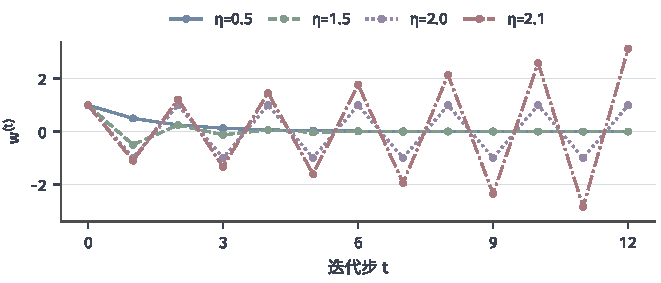
\includegraphics[width=112mm]{figures/01-mathematical-preliminaries-upper/01-mathematical-language-combinatorics-analysis-optimization/matplotlib/comprehension-additions/gradient-step-stability.pdf}
  \caption{对$f(w)=w^2/2$取$w^{(0)}=1$，画精确迭代$w^{(t)}=(1-\eta)^t$。$\eta=0.5$同侧收缩，$\eta=1.5$换侧收缩，$\eta=2$等幅振荡，$\eta=2.1$幅度增长。各点仅对应整数步，连线帮助追踪次序。这里$L=1$，稳定边界正是$2/L$。}
  \label{fig:vol1-add-gradient-step-stability}
\end{figure}

若$f$还凸、最小点$\bm{w}^{\star}$存在，并继续取$\eta=1/L$，则由凸性有
$f(\bm{w}^{(t)})-f^\star
\leq\langle\nabla f(\bm{w}^{(t)}),\bm{w}^{(t)}-\bm{w}^{\star}\rangle$。
先展开距离平方并使用这个不等式：
\begin{align*}
  \lVert\bm{w}^{(t+1)}-\bm{w}^{\star}\rVert_2^2
  &=
  \lVert\bm{w}^{(t)}-\bm{w}^{\star}\rVert_2^2
  -\frac{2}{L}
  \left\langle\nabla f(\bm{w}^{(t)}),
  \bm{w}^{(t)}-\bm{w}^{\star}\right\rangle\\
  &\qquad
  +\frac{1}{L^2}\lVert\nabla f(\bm{w}^{(t)})\rVert_2^2\\
  &\leq
  \lVert\bm{w}^{(t)}-\bm{w}^{\star}\rVert_2^2
  -\frac{2}{L}\bigl(f(\bm{w}^{(t)})-f^\star\bigr)\\
  &\qquad
  +\frac{1}{L^2}\lVert\nabla f(\bm{w}^{(t)})\rVert_2^2.
\end{align*}
另一方面，把$\eta=1/L$代入式~\eqref{eq:opt-gradient-single-step}可得
\[
  \frac{1}{L^2}\lVert\nabla f(\bm{w}^{(t)})\rVert_2^2
  \leq
  \frac{2}{L}\bigl(
  f(\bm{w}^{(t)})-f(\bm{w}^{(t+1)})\bigr).
\]
用后一式消去梯度平方项，得到
\[
  \lVert\bm{w}^{(t+1)}-\bm{w}^{\star}\rVert_2^2
  \leq
  \lVert\bm{w}^{(t)}-\bm{w}^{\star}\rVert_2^2
  -\frac{2}{L}\bigl(f(\bm{w}^{(t+1)})-f^\star\bigr).
\]
对$t=0,\ldots,T-1$求和并去掉末端的非负距离，便有
\[
  \frac{2}{L}\sum_{t=0}^{T-1}
  \bigl(f(\bm{w}^{(t+1)})-f^\star\bigr)
  \leq
  \lVert\bm{w}^{(0)}-\bm{w}^{\star}\rVert_2^2.
\]
式~\eqref{eq:opt-gradient-single-step}还说明目标值单调不增，因此左侧求和中的每一项
都不小于$f(\bm{w}^{(T)})-f^\star$。于是
\begin{equation}
  f(\bm{w}^{(T)})-f^\star
  \leq\frac{L\lVert\bm{w}^{(0)}-\bm{w}^{\star}\rVert_2^2}{2T}.
  \label{eq:opt-convex-gradient-rate}
\end{equation}

\term{Polyak--Łojasiewicz条件}（PL condition）不约束函数图像必须凸，而用梯度大小控制
距离最优值还有多少差距。
\begin{definition}[Polyak--Łojasiewicz条件]
\label{def:opt-pl-condition}
设$f:\mathbb{R}^d\to\mathbb{R}$可微，$f^\star=\inf_{\bm{w}}f(\bm{w})> -\infty$。
若存在$\mu>0$，使任意$\bm{w}$满足
\begin{equation}
  \frac{1}{2}\lVert\nabla f(\bm{w})\rVert_2^2
  \geq \mu\bigl(f(\bm{w})-f^{\star}\bigr),
  \qquad \mu>0.
  \label{eq:opt-pl-condition}
\end{equation}
则称$f$满足常数为$\mu$的PL条件。
\end{definition}
该条件把小梯度与小目标误差联系起来。强凸可推出PL条件：对$\mu$强凸可微函数，把强凸
下界右侧关于$\bm{v}$最小化，得到
\[
  f^\star\geq
  f(\bm{w})-\frac{1}{2\mu}\lVert\nabla f(\bm{w})\rVert_2^2,
\]
移项正是式~\eqref{eq:opt-pl-condition}。这个推导使用全局强凸下界；只有局部Hessian
正定时，不能直接得到全域PL条件。反过来，PL函数可以有多个最小点。

PL条件也确实可以出现在非凸函数中。考虑
\[
  f(x,y)=x^2+2\sin^2x.
\]
它与$y$无关，因而最小点不唯一。其一阶导数为
$\partial f/\partial x=2(x+\sin 2x)$；当$x>0$时，若$x\leq1$则两项均非负，
若$x>1$则$x+\sin2x\geq x-1>0$，负半轴由奇对称性处理，所以导数只在$x=0$时
为零。比值
\[
  R(x)=\frac{\lVert\nabla f(x,y)\rVert_2^2}{2f(x,y)}
\]
在$x\neq0$时为正，并且$x\to0$时趋于$6$，$|x|\to\infty$时趋于$2$。
把两端之外的剩余区域限制为紧集，连续函数$R$在其中有正下界，故某个$\mu>0$使
式~\eqref{eq:opt-pl-condition}成立。另一方面，
$\partial^2 f/\partial x^2=2+4\cos2x$在某些点为负，所以$f$并不凸；该二阶导数
下界为$-2$、绝对值上界为$6$，所以它仍是$6$光滑的。负曲率下界的另一用途将在
邻近方法中解释；这里的例子表明非凸性本身不排斥目标值的梯度控制。

应用PL条件时，可将已有常数减小到$0<\mu\leq L$；这不会破坏原不等式，并使下面的收缩因子非负。把式~\eqref{eq:opt-pl-condition}代入
式~\eqref{eq:opt-gradient-single-step}，在$\eta=1/L$时得到
\begin{equation}
  f(\bm{w}^{(t)})-f^\star
  \leq
  \left(1-\frac{\mu}{L}\right)^t
  \bigl(f(\bm{w}^{(0)})-f^\star\bigr).
  \label{eq:opt-pl-linear-rate}
\end{equation}
强凸函数满足PL条件，还由
$f(\bm{w})-f^\star\geq\mu\lVert\bm{w}-\bm{w}^{\star}\rVert_2^2/2$
把目标误差转成参数误差。没有强凸时，式~\eqref{eq:opt-pl-linear-rate}不保证迭代趋向
某个唯一参数。

固定步长需要已知或估计$L$，而真实问题的$L$往往只能上界估计或完全未知；估计偏大时步长过小、收敛变慢，估计偏小时下降保证失效。一种不依赖$L$具体数值的做法是先用实际函数值检验当前这一步是否真的下降了。回溯线搜索从候选步长开始缩小，直到
$f(\bm{w}-\eta\nabla f(\bm{w}))\leq
f(\bm{w})-c\eta\lVert\nabla f(\bm{w})\rVert_2^2$成立，其中$c\in(0,1)$。
学习率调度则预先或按进度改变$\eta^{(t)}$。线搜索用实际函数值核验当前一步，调度只规定时间
表；二者都不能弥补错误梯度或无下界目标。

具体执行回溯时，给定初始试探步长$\bar\eta>0$、缩减比例$\gamma\in(0,1)$与$c\in(0,1)$。
每轮先算一次$\bm g=\nabla f(\bm w)$，若$\|\bm g\|_2$已满足停止要求就返回；
否则从$\eta=\bar\eta$开始，计算候选$\bm w-\eta\bm g$的函数值，若未满足上述充分下降条件，
令$\eta\leftarrow\gamma\eta$再试，接受后进入下一轮。下降引理保证
$\eta\leq2(1-c)/L$时一定通过，所以全局$L$光滑时每轮有限次结束，
接受步长至少为$\min\{\bar\eta,2\gamma(1-c)/L\}$。
增加的成本主要是试探点函数求值，而非每次重算当前位置的梯度。

在式~\eqref{eq:opt-common-quadratic}中，$\eta=1/16$给
$\bm w^{(t)}=(2(15/16)^t,0)^\top$（$t\geq1$），于是
$f(\bm w^{(t)})=2(15/16)^{2t}$。第二坐标一步消去，第一坐标却受较大曲率限制而缓慢缩小。
$\eta=0.1$使两坐标分别乘$0.9$与$-0.6$，目标仍下降但路径振荡；
$\eta=1/8$使第二坐标等幅振荡，$\eta>1/8$使它发散。
一般非凸问题返回梯度范数最小的已访问点，式~\eqref{eq:opt-nonconvex-gradient-rate}
控制其驻点残差；凸问题可返回最后一点并用式~\eqref{eq:opt-convex-gradient-rate}控制目标差。
已知PL常数时，$\|\nabla f\|_2\leq\sqrt{2\mu\varepsilon}$足以保证目标差不超过$\varepsilon$；
不能将这条停止规则无条件用于所有光滑目标。

\subsubsection{基于动量与加速的求解}
\label{sec:opt-curvature-acceleration}

对二次函数$f(\bm{w})=\frac12\bm{w}^{\top}\bm{H}\bm{w}
-\bm{c}^{\top}\bm{w}$，设$\bm H\succ\bm 0$，则唯一最小点为$\bm w^\star=\bm H^{-1}\bm c$。
记误差$\bm e^{(t)}=\bm w^{(t)}-\bm w^\star$；由$\nabla f(\bm w)=\bm H(\bm w-\bm w^\star)$，
梯度下降的误差满足
$\bm{e}^{(t+1)}=(\bm{I}-\eta\bm{H})\bm{e}^{(t)}$。沿$\bm H$的特征方向分解，曲率为
$\lambda_i$的误差分量每步乘以$1-\eta\lambda_i$。记最大、最小曲率为
$L=\lambda_{\max}(\bm H)$、$\mu=\lambda_{\min}(\bm H)$，条件数为$\kappa=L/\mu$。
陡峭方向要求$\eta<2/L$，于是最平坦方向每步只能把误差乘以$1-\eta\mu>1-2/\kappa$；
$\kappa$很大时，同一步长必须同时照顾陡峭与平坦方向，平坦方向因而收敛缓慢。

在狭长谷底上，梯度方向在两侧之间来回摆动，真正指向谷底的方向分量却每步都很小；
想象一个小球在又陡又窄的滑槽里下滑：它大部分动能用于在两壁之间左右撞击，沿槽向谷底
前进却很慢。对梯度逐步取平均，摆动分量相消，有效方向便指向谷底。这是保留历史方向的作用。
\term{动量法}（momentum method）保存过去方向，使连续几步指向同一侧的梯度能够累积。
这里采用重球（heavy-ball）形式：
\[
  \bm{v}^{(t+1)}=\beta\bm{v}^{(t)}+\nabla f(\bm{w}^{(t)}),
  \qquad
  \bm{w}^{(t+1)}=\bm{w}^{(t)}-\eta\bm{v}^{(t+1)}.
\]
取$\bm v^{(0)}=0$，或等价地令$\bm w^{(-1)}=\bm w^{(0)}$，即可启动重球迭代。
每轮只需一次当前位置梯度、一个历史方向和向量加法；它没有计算Hessian。
消去$\bm v$可得$\bm w^{(t+1)}=\bm w^{(t)}-\eta\nabla f(\bm w^{(t)})
+\beta(\bm w^{(t)}-\bm w^{(t-1)})$，
所以对上述正定二次目标，曲率为$\lambda_i$的特征方向上的误差分量满足
\[
  e_i^{(t+1)}
  =(1+\beta-\eta\lambda_i)e_i^{(t)}-\beta e_i^{(t-1)}.
\]
梯度下降的新误差只由上一步决定，$t$步后的误差分量等于初始值乘以$(1-\eta\lambda_i)^t$；
历史项使新误差同时依赖前两步，$t$步后的乘数成为另一个关于$\eta\lambda_i$的$t$次多项式。
选择$\beta$和$\eta$就是在调整这个多项式在各曲率上的大小，二者不能各自独立地任取。
该方向的两个特征根都严格位于单位圆内，当且仅当
$-1<\beta<1$且$0<\eta\lambda_i<2(1+\beta)$。因而常用的
$0\leq\beta<1$还须配合$0<\eta<2(1+\beta)/L$，才能保证所有方向稳定。
若已知$0<\mu\leq\lambda_i\leq L$，经典重球参数
\[
  \eta=\frac{4}{(\sqrt{L}+\sqrt{\mu})^2},
  \qquad
  \beta=\left(\frac{\sqrt{L}-\sqrt{\mu}}
  {\sqrt{L}+\sqrt{\mu}}\right)^2
\]
给出这一二次模型上的代表性最坏方向速率；它不是一般非凸目标或含噪梯度下的无条件
调参规则。
稳定区间也可从特征多项式
$r^2-(1+\beta-\eta\lambda_i)r+\beta$核对：实系数二次多项式的两根在单位圆内，
等价于$|\beta|<1$、$\eta\lambda_i>0$与$2+2\beta-\eta\lambda_i>0$。
经典参数的根模至多
$q=(\sqrt L-\sqrt\mu)/(\sqrt L+\sqrt\mu)$，端点的重根会带来$tq^t$因子；
因此不能不带常数地把有限步参数误差写成$q^t$。
在共同二次例上，$\eta=4/25$、$\beta=9/25$且零初速度给出精确轨迹
\[
 w_1^{(t)}=(2+0.8t)\,0.6^t,\qquad
 w_2^{(t)}=(2+3.2t)(-0.6)^t.
\]
第一步为$(1.68,-3.12)$，目标从$34$升至$79.2864$，之后仍趋于零。
重球的稳定和渐近提速不等于逐步下降；给定有限预算时要连同启动阶段比较。

\term{Nesterov加速梯度}
（Nesterov accelerated gradient）在前瞻点计算梯度：
\[
 \bm w^{(t+1)}=\bm z^{(t)}-\frac1L\nabla f(\bm z^{(t)}),\qquad
 q^{(t+1)}=\frac{1+\sqrt{1+4(q^{(t)})^2}}2,
\]
\[
 \bm z^{(t+1)}=\bm w^{(t+1)}
 +\frac{q^{(t)}-1}{q^{(t+1)}}(\bm w^{(t+1)}-\bm w^{(t)}).
\]
初始化为$\bm z^{(0)}=\bm w^{(0)}$、$q^{(0)}=1$。必须先得到新点，再形成下一轮前瞻点；
不能把下一轮外推系数提前用于本轮。
若$f$为凸可微函数、梯度$L$-Lipschitz连续、最小点存在，并且每步使用精确梯度和
步长$1/L$，则对$T\geq1$，
\begin{equation}
 f(\bm w^{(T)})-f^\star
 \leq\frac{2L\|\bm w^{(0)}-\bm w^\star\|_2^2}{(T+1)^2}.
 \label{eq:opt-accelerated-finite-rate}
\end{equation}
同样条件下，普通梯度下降的一般保证为$O(1/T)$。
强凸时可以另取固定外推系数
$\beta=(\sqrt L-\sqrt\mu)/(\sqrt L+\sqrt\mu)$与步长$1/L$，
获得$O((1-\sqrt{\mu/L})^T)$的目标误差界；这不是重球的步长参数。
在一维二次函数$f(w)=\lambda w^2/2$上，上述一般凸加速迭代可直接核验为
\[
  w^{(t+1)}
  =\left(1-\frac{\lambda}{L}\right)
  \bigl((1+\beta^{(t)})w^{(t)}-\beta^{(t)} w^{(t-1)}\bigr).
\]
其中$t\geq1$时$\beta^{(t)}=(q^{(t-1)}-1)/q^{(t)}$，初始化时取$\beta^{(0)}=0$。
当$\lambda=L$时一步到达零点；当$\lambda\ll L$时，跨步项改变平坦方向上的二阶递推，
但系数选错仍会振荡。二次算例不能代替一般保证，下面用势函数证明一般凸情形的界：
势函数是把目标差与到最小点的距离合在一起的非负分析量，算法本身不必计算它；
只要证明它每步不增，就能由初值读出最后的误差界。
对$\bm x^+=\bm z-\nabla f(\bm z)/L$，下降引理给$f(\bm x^+)\leq f(\bm z)-\|\nabla f(\bm z)\|_2^2/(2L)$，
凸性给$f(\bm z)\leq f(\bm v)+\langle\nabla f(\bm z),\bm z-\bm v\rangle$。两式相加，
代入$\nabla f(\bm z)=L(\bm z-\bm x^+)$并配方，得到对任意$\bm v$成立的三点不等式
\[
 f(\bm x^+)-f(\bm v)
 \leq\frac L2\bigl(\|\bm v-\bm z\|_2^2-\|\bm v-\bm x^+\|_2^2\bigr).
\]
要让相邻两步的目标差与距离项相接，我们选择一个位于当前点与最小点之间的比较点。
比较点只用于证明，不是算法需要求出的点。权重取$1/q^{(t)}$，是为了在稍后乘以
$(q^{(t)})^2$时，把旧目标差的系数变成$q^{(t)}(q^{(t)}-1)$，与$q$的递推对应。
递推使$q^{(t)}\geq1$，因而下面确为凸组合：
$\bm v=(1-1/q^{(t)})\bm w^{(t)}+\bm w^\star/q^{(t)}$。
记$\Delta^{(t)}=f(\bm w^{(t)})-f^\star$，凸性给$f(\bm v)-f^\star\leq(1-1/q^{(t)})\Delta^{(t)}$。
把$\bm z=\bm z^{(t)}$、$\bm x^+=\bm w^{(t+1)}$代入三点不等式，得到
\[
 \Delta^{(t+1)}
 \leq\Bigl(1-\frac1{q^{(t)}}\Bigr)\Delta^{(t)}
 +\frac L2\bigl(\|\bm v-\bm z^{(t)}\|_2^2-\|\bm v-\bm w^{(t+1)}\|_2^2\bigr).
\]
三点不等式中的两项距离还分别涉及外推点与新迭代点。
把它们都乘以$q^{(t)}$后，可以用同一种辅助点表示相邻状态：令
$\bm u^{(t+1)}=q^{(t)}\bm w^{(t+1)}-(q^{(t)}-1)\bm w^{(t)}
=\bm w^{(t+1)}+(q^{(t)}-1)(\bm w^{(t+1)}-\bm w^{(t)})$及$\bm u^{(0)}=\bm w^{(0)}$。
它把外推位移合并进一个向量，只用于追踪误差，不增加算法所需的状态或梯度计算。
由$q^{(t)}\bm v=(q^{(t)}-1)\bm w^{(t)}+\bm w^\star$可得
$q^{(t)}(\bm v-\bm w^{(t+1)})=\bm w^\star-\bm u^{(t+1)}$；
把$\bm z^{(t)}$的外推定义展开，又有$q^{(t)}\bm z^{(t)}-(q^{(t)}-1)\bm w^{(t)}=\bm u^{(t)}$，
故$q^{(t)}(\bm v-\bm z^{(t)})=\bm w^\star-\bm u^{(t)}$。上式乘以$(q^{(t)})^2$后得到
\[
 (q^{(t)})^2\Delta^{(t+1)}+\frac L2\|\bm u^{(t+1)}-\bm w^\star\|_2^2
 \leq q^{(t)}(q^{(t)}-1)\Delta^{(t)}+\frac L2\|\bm u^{(t)}-\bm w^\star\|_2^2.
\]
将左侧记为$E^{(t+1)}$：它把加权目标差与辅助点到最小点的距离平方相加。
取$E^{(0)}=L\|\bm w^{(0)}-\bm w^\star\|_2^2/2$。
先核对启动时的两次比较。$q^{(0)}=1$使$\bm u^{(1)}=\bm w^{(1)}$，
而$q^{(1)}(q^{(1)}-1)=1$，所以
\[
\begin{aligned}
 E^{(1)}&=\Delta^{(1)}+\frac L2\|\bm w^{(1)}-\bm w^\star\|_2^2
          \leq E^{(0)},\\
 E^{(2)}&=(q^{(1)})^2\Delta^{(2)}
          +\frac L2\|\bm u^{(2)}-\bm w^\star\|_2^2
          \leq E^{(1)}.
\end{aligned}
\]
一般$t\geq1$时，同一恒等式
$q^{(t)}(q^{(t)}-1)=(q^{(t-1)})^2$
使右侧恰为$E^{(t)}$。这就是选取比较点权重和辅助点的作用：旧目标差的系数与旧距离项
一起组成上一步的势函数，而非分别估计两个互不相接的误差。
故$(q^{(T-1)})^2\Delta^{(T)}\leq L\|\bm w^{(0)}-\bm w^\star\|_2^2/2$。
递推又给$q^{(T-1)}\geq(T+1)/2$，即得式~\eqref{eq:opt-accelerated-finite-rate}。
每轮代价仍是一次梯度与几个向量操作，但目标未必单调；一般凸情形的目标收敛也没有规定
唯一参数。强凸时才可再用式~\eqref{eq:opt-strong-convex-distance}转成参数界。

\subsection{基于二阶信息的求解}
\label{sec:opt-second-order-methods}

在共同二次例子中，两坐标的曲率相差$16$倍，一个标量步长必须兼顾两个方向：步长大到够快消去平坦方向，陡峭方向就会振荡。
用一个物理类比理解二阶方法：梯度只告诉你当前往哪边倾斜，而曲率告诉你“再往前走一步，
坡面会转多少”。一阶方法用同一个步长对待所有方向，在缓坡上走得太慢、在陡坡上又容易
冲过头；若在局部模型中保留不同方向的曲率，就能分别调整位移，这是一阶方向之外的另一种计算选择。二阶方法需要取得或近似曲率矩阵，并求解相应方程；更准确的局部模型也带来额外计算成本。本节先看直接构造曲率模型的做法，再看只从梯度差近似曲率的做法，最后看不改变曲率模型、只改变度量尺度的预条件。

\subsubsection{基于牛顿与Gauss–Newton更新的求解}
\label{sec:opt-newton-gauss-newton}

第~\ref{chap:multivariate-calculus}章的二阶展开把当前点附近的目标近似为关于位移$\bm p$的二次函数。曲率矩阵正定时，这个模型有唯一最小点，可以用该点的位移作为更新方向。\term{牛顿法}（Newton's method）由模型的驻点方程求出这一方向；曲率不正定时，方程解的含义需要另行核对。在当前参数$\bm w^{(t)}$处，模型为
\[
  m^{(t)}(\bm{p})
  =
  f(\bm{w}^{(t)})
  +\left\langle\nabla f(\bm{w}^{(t)}),\bm{p}\right\rangle
  +\frac12\bm{p}^{\top}\nabla^2f(\bm{w}^{(t)})\bm{p}.
\]
令$\nabla_{\bm{p}}m^{(t)}(\bm{p}^{(t)})=\bm{0}$，便得到牛顿方程
\[
  \nabla^2 f(\bm{w}^{(t)})\bm{p}^{(t)}
  =-\nabla f(\bm{w}^{(t)}),\qquad
  \bm{w}^{(t+1)}=\bm{w}^{(t)}+\alpha^{(t)}\bm{p}^{(t)}.
\]
若Hessian矩阵在最优点附近正定且Lipschitz连续，取单位步长可得到局部二次收敛。但Hessian矩阵
不定时，牛顿方向未必下降；离最优点较远时还需线搜索或信赖域。
可逆性只使方程有唯一解，正定性才使这个解成为二次模型的最小点。
实际过程是计算梯度与Hessian，求解线性方程得到$\bm p^{(t)}$，核验其下降性，再选择步长。
若Hessian不正定，可用$\nabla^2f+\delta^{(t)}\bm I\succ0$替代它；沿该方向执行充分下降线搜索，
而不是直接接受单位步长。奇异Hessian下也不能照写逆矩阵。

牛顿法的代价来自三处，都应在选用前核算：一是需要算出$d\times d$个二阶偏导数，
二是每轮要解一个线性方程，三是只能保证局部收敛。若梯度和曲率本身需要抽样估计，
这三项成本还会叠加。下面的界量化的是第三项。

局部二次速率有可量化的范围。设$\nabla f(\bm w^\star)=0$，在包含$\bm w^\star$的球内
$\nabla^2f(\bm w)\succeq m\bm I$且Hessian为$M$-Lipschitz，其中$m>0$。
对单位牛顿步，令$\bm e=\bm w-\bm w^\star$，沿线段积分梯度得
\[
 \bm e^+
 =\nabla^2f(\bm w)^{-1}\!
 \int_0^1\bigl(\nabla^2f(\bm w)-\nabla^2f(\bm w^\star+s\bm e)\bigr)\bm e\,ds,
 \quad
 \|\bm e^+\|_2\leq\frac{M}{2m}\|\bm e\|_2^2.
\]
初始误差足够小，使这个界将点留在同一球内，才可逐轮使用。
共同二次例的Hessian恒定，$M=0$，求解$\bm H\bm p=-\bm H\bm w$得到
$\bm p=-\bm w$，一步到达零点。一般稠密$d$维问题需要存储$O(d^2)$个矩阵元素，
直接分解约需$O(d^3)$运算；本例的对角结构才把这一成本降为$O(d)$。

对非线性最小二乘
$f(\bm{w})=\frac12\lVert\bm{r}(\bm{w})\rVert_2^2$，设
$\bm{r}:\mathbb{R}^d\to\mathbb{R}^m$二阶可微。记残差向量的Jacobian矩阵为
$\bm{J}(\bm{w})\in\mathbb{R}^{m\times d}$，其第$i$行为
$\bm{J}_{i,:}(\bm{w})=\nabla r_i(\bm{w})^{\top}$，则
\[
  \nabla^2f(\bm{w})
  =\bm{J}(\bm{w})^{\top}\bm{J}(\bm{w})
  +\sum_{i=1}^m r_i(\bm{w})\nabla^2r_i(\bm{w}).
\]
\term{Gauss--Newton法}忽略第二项，使用半正定矩阵
$\bm{J}^{\top}\bm{J}$。当残差小或残差函数近似线性时近似合理；残差大时，省略项可能
决定曲率。
它的方向不是凭空替换矩阵，而是先线性化残差，求解
\[
 \min_{\bm p}\frac12\|\bm r(\bm w)+\bm J(\bm w)\bm p\|_2^2,
 \qquad
 \bm J^\top\bm J\bm p=-\bm J^\top\bm r.
\]
残差Jacobian描述每个残差对参数的变化，Hessian描述整个标量目标的曲率，两者维度也不同。
$\bm J$满列秩时子问题方向唯一；秩亏时可用QR或奇异值分解取最小范数方向，
也可增加$\delta\|\bm p\|_2^2/2$得到
$(\bm J^\top\bm J+\delta\bm I)\bm p=-\bm J^\top\bm r$。
对未正则化子问题，直接形成正规方程会平方条件数，数值实现常直接解线性最小二乘。

若解附近$\bm J$满列秩且Lipschitz、残差在解处为零，则
$\bm r(\bm w)=\bm J(\bm w)(\bm w-\bm w^\star)+O(\|\bm w-\bm w^\star\|_2^2)$，
左逆一致有界便给出局部二次误差。非零残差时，把一次Gauss--Newton更新看成从当前参数到
下一步参数的迭代映射
\[
 \bm G(\bm w)=\bm w-\bigl(\bm J(\bm w)^\top\bm J(\bm w)\bigr)^{-1}\bm J(\bm w)^\top\bm r(\bm w),
 \qquad \bm w^{(t+1)}=\bm G(\bm w^{(t)}).
\]
设局部解$\bm w^\star$附近$\bm J$满列秩、各残差二阶连续可微，记$\bm J^\star=\bm J(\bm w^\star)$、
$\bm E^\star=\sum_i r_i(\bm w^\star)\nabla^2r_i(\bm w^\star)$。驻点满足
$\nabla f(\bm w^\star)=\bm J^{\star\top}\bm r(\bm w^\star)=\bm 0$。对乘积
$(\bm J^\top\bm J)^{-1}\nabla f$求导时，作用在逆矩阵上的项乘以$\nabla f(\bm w^\star)=\bm0$而消失，
只剩$(\bm J^{\star\top}\bm J^\star)^{-1}\nabla^2f(\bm w^\star)$；代入前面的Hessian分解得
\[
 \bm D\bm G(\bm w^\star)
 =\bm I-(\bm J^{\star\top}\bm J^\star)^{-1}\bigl(\bm J^{\star\top}\bm J^\star+\bm E^\star\bigr)
 =-(\bm J^{\star\top}\bm J^\star)^{-1}\bm E^\star.
\]
零残差时$\bm E^\star=\bm 0$，这个导数矩阵为零，与二次误差一致。非零残差时，若它在某个
向量范数诱导的矩阵范数下小于$1$，导数的连续性使$\bm G$在$\bm w^\star$的某个小球内成为
压缩映射，从球内出发的迭代局部线性收敛。这只是充分条件，速率通常只是线性的；
残差大或秩条件失效时不能保证收敛。共同二次例可取
$\bm r(\bm w)=(w_1,4w_2)^\top$，残差本身线性，Gauss--Newton与牛顿方向完全一致。

\paragraph{残差线性化下的阻尼控制}
\label{sec:opt-levenberg-marquardt}

线性化只在当前点附近可靠，解出子问题还不足以决定是否接受这一步。\term{Levenberg--Marquardt法}（Levenberg--Marquardt method）先限制位移，再比较真实下降与模型预报，借此调整下一次试探的尺度\scite{math-nocedal2006numerical,math-ceres-nnls}在当前点省略迭代上标，记$\bm r=\bm r(\bm w)$、$\bm J=\bm J(\bm w)$，考虑
\[
 m(\bm p)=\tfrac12\|\bm r+\bm J\bm p\|_2^2,
 \qquad
 \min_{\bm p}m(\bm p)+\tfrac\mu2\|\bm p\|_2^2,
 \quad\mu>0.
\]
它给出前面的阻尼方程$(\bm J^\top\bm J+\mu\bm I)\bm p=-\bm J^\top\bm r$。即使$\bm J$秩亏，新增项也使步长子问题严格凸。这里惩罚的是本轮位移$\bm p$，没有把原目标永久改为$f(\bm w)+\mu\|\bm w\|_2^2/2$。由方程与$\bm p$作内积，可得$\mu\|\bm p\|_2\leq\|\bm J^\top\bm r\|_2$；增大阻尼因此限制本轮移动，但不能恢复观测中本来缺失的信息。

同一方程也联系信赖域问题$\min m(\bm p)$、$\|\bm p\|_2\leq\Delta$。其乘子条件为
\[
 (\bm J^\top\bm J+\mu\bm I)\bm p=-\bm J^\top\bm r,
 \quad \mu\geq0,
 \quad \mu(\|\bm p\|_2^2-\Delta^2)=0.
\]
对$\mu>0$算出的非零步，取$\Delta=\|\bm p\|_2$便满足这些凸子问题的充分最优条件。预先固定半径时，则需选择与它相容的阻尼，不能把任意$\mu$称为该半径的精确解。实际实现也可用正对角矩阵缩放不同单位的参数；下面只讨论单位矩阵形式。

接受与否应回到原目标。若模型预报下降$\operatorname{pred}=m(\bm0)-m(\bm p)>0$，计算
\begin{equation}
 \rho=\frac{f(\bm w)-f(\bm w+\bm p)}{m(\bm0)-m(\bm p)}.
 \label{eq:opt-lm-reduction-ratio}
\end{equation}
分母不包含步长惩罚，因为要核对的是原残差模型对原目标的预报。取$0<\eta<1/4$，一种简明规则是：$\rho>\eta$时接受新点，否则保留当前点；$\rho<1/4$时把阻尼乘四，$\rho>3/4$时把阻尼减半，其余情况保持阻尼。拒绝后在同一点重算方向和预报。若预报非正，先增大阻尼重试；梯度已为零时应报告驻点检查，不能用零分母计算比值。具体阈值有多种选择，以上规则说明各次试探怎样连起来，不单凭这套规则宣称全局最优或无条件收敛。

这一区别可以直接核算。令$r(w)=w^2-4$、$w=1/2$，则$r=-15/4$、$J=1$，无阻尼步为$p=15/4$；新点$17/4$使目标从$225/32$升为$50625/512$。取$\mu=4$时，步长改为$3/4$，新点$5/4$的目标为$1521/512<225/32$。模型预报下降为$81/32$，真实下降为$2079/512$，比值为$77/48>1$：这一步的模型预报偏保守，但确实降低了原目标。阻尼不是只让方程可逆，还用于控制线性化误差。


\subsubsection{基于拟牛顿更新的求解}
\label{sec:opt-quasi-newton}

完整Hessian可能难以获得，但走过一步后，已经知道位移与梯度变化。
\term{拟牛顿法}（quasi-Newton method）用这两份信息修正曲率模型，不显式计算Hessian矩阵。
记位移$\bm{s}^{(t)}=\bm{w}^{(t+1)}-\bm{w}^{(t)}$与梯度差
$\bm{y}^{(t)}=\nabla f(\bm{w}^{(t+1)})-\nabla f(\bm{w}^{(t)})$；位移是向量，
不同于后面线搜索中的标量步长。若$f$二阶连续可微，沿这段位移对梯度积分得
\[
 \bm y^{(t)}=\left(\int_0^1\nabla^2f(\bm w^{(t)}+\tau\bm s^{(t)})\,d\tau\right)\bm s^{(t)},
\]
对二次目标则恰有$\bm y^{(t)}=\bm H\bm s^{(t)}$。梯度差因而记录了Hessian沿刚走过方向的平均作用。
拟牛顿法要求新的近似矩阵至少复现这一观测，即满足割线条件
$\bm{B}^{(t+1)}\bm{s}^{(t)}=\bm{y}^{(t)}$。一维时它要求近似二阶导数等于导函数在两点间的
差商，也就是导函数图像上割线的斜率，名称由此而来。位移非零且$d\geq2$时，满足割线条件的对称矩阵不止一个。
若$\bm{B}^{(t)}$是当前的Hessian近似，Broyden--Fletcher--Goldfarb--Shanno（BFGS）更新
保持对称，并只用两个秩一项修正$\bm B^{(t)}$：
\begin{equation}
  \bm{B}^{(t+1)}
  =
  \bm{B}^{(t)}
  +
  \frac{\bm{y}^{(t)}(\bm{y}^{(t)})^{\top}}
       {(\bm{y}^{(t)})^{\top}\bm{s}^{(t)}}
  -
  \frac{\bm{B}^{(t)}\bm{s}^{(t)}(\bm{s}^{(t)})^{\top}\bm{B}^{(t)}}
       {(\bm{s}^{(t)})^{\top}\bm{B}^{(t)}\bm{s}^{(t)}}.
  \label{eq:opt-bfgs-update}
\end{equation}
当$\bm{B}^{(t)}\succ\bm{0}$且曲率条件
$(\bm{y}^{(t)})^{\top}\bm{s}^{(t)}>0$成立时，
式~\eqref{eq:opt-bfgs-update}保持$\bm{B}^{(t+1)}\succ\bm{0}$，相应搜索方向
$-(\bm{B}^{(t+1)})^{-1}\nabla f$才由正定性保证是下降方向。沿下降方向执行满足
Wolfe条件的线搜索可产生该正曲率内积。具体地，令
$\bm{w}^{(t+1)}=\bm{w}^{(t)}+\alpha^{(t)}\bm{p}^{(t)}$，其中
$\nabla f(\bm{w}^{(t)})^{\top}\bm{p}^{(t)}<0$。Wolfe条件要求存在
$0<c_1<c_2<1$使
\begin{equation}
\begin{aligned}
  f(\bm{w}^{(t+1)})
  &\leq
  f(\bm{w}^{(t)})
  +
  c_1\alpha^{(t)}
  \nabla f(\bm{w}^{(t)})^{\top}\bm{p}^{(t)},\\
  \nabla f(\bm{w}^{(t+1)})^{\top}\bm{p}^{(t)}
  &\geq
  c_2\nabla f(\bm{w}^{(t)})^{\top}\bm{p}^{(t)}.
\end{aligned}
\label{eq:opt-wolfe-conditions}
\end{equation}
第二行就是\term{Wolfe曲率条件}（Wolfe curvature condition）。由
$\bm{s}^{(t)}=\alpha^{(t)}\bm{p}^{(t)}$可得
\[
  (\bm{y}^{(t)})^{\top}\bm{s}^{(t)}
  \geq
  \alpha^{(t)}(c_2-1)
  \nabla f(\bm{w}^{(t)})^{\top}\bm{p}^{(t)}
  >0.
\]
非凸或梯度含噪时，上述条件可能难以满足，此时可能需要阻尼或跳过更新。

正定性的理由值得单独核验。省略轮次上标，对任意$\bm v\neq0$，
\[
 \bm v^\top\bm B^+\bm v
 =\bm v^\top\bm B\bm v
 -\frac{(\bm v^\top\bm B\bm s)^2}{\bm s^\top\bm B\bm s}
 +\frac{(\bm v^\top\bm y)^2}{\bm y^\top\bm s}.
\]
前两项由$\bm B$内积的Cauchy--Schwarz不等式非负，仅在$\bm v$与$\bm s$平行时为零；
此时$\bm y^\top\bm s>0$又使最后一项严格为正。把更新式乘$\bm s$，
还可直接检查$\bm B^+\bm s=\bm y$。割线条件只匹配一个观测方向，不等于已经恢复全部曲率。

一次BFGS迭代从正定$\bm B^{(t)}$出发，解
$\bm B^{(t)}\bm p^{(t)}=-\nabla f(\bm w^{(t)})$，进行Wolfe线搜索，计算新梯度与
$(\bm s^{(t)},\bm y^{(t)})$后再更新矩阵。仅用不断缩短步长的Armijo回溯未必满足
Wolfe第二式，因为步长太小会使方向导数几乎不变；需要括住合适步长区间再缩小区间。
若观测曲率太小，给定$\delta\in(0,1)$，可以令
\[
 \widetilde{\bm y}=\theta\bm y+(1-\theta)\bm B\bm s,\qquad
 \theta=
 \begin{cases}
 1,&\bm s^\top\bm y\geq\delta\bm s^\top\bm B\bm s,\\
 \dfrac{(1-\delta)\bm s^\top\bm B\bm s}
 {\bm s^\top\bm B\bm s-\bm s^\top\bm y},&\text{其余情形}.
 \end{cases}
\]
用$\widetilde{\bm y}$替代$\bm y$便有
$\bm s^\top\widetilde{\bm y}\geq\delta\bm s^\top\bm B\bm s>0$；
代价是割线条件改为匹配修正后的曲率。零位移或不可靠梯度差应跳过更新。

牛顿法每轮都要解一个线性方程，直接分解稠密矩阵的代价是$O(d^3)$。若维护的是逆矩阵的
近似，只需一次矩阵向量乘法就能得到方向，每轮代价降为$O(d^2)$；这正是拟牛顿法更新
逆矩阵而不是更新$\bm B$并求解的原因。为避免每轮重新分解稠密矩阵，通常维护
$\bm C=\bm B^{-1}$并用等价公式
\[
 \bm C^+=(\bm I-\rho\bm s\bm y^\top)\bm C
          (\bm I-\rho\bm y\bm s^\top)+\rho\bm s\bm s^\top,
 \qquad \rho=(\bm y^\top\bm s)^{-1}.
\]
方向是$-\bm C\nabla f$，更新与乘法各需$O(d^2)$运算和存储；
有限记忆版本只保存最近$m$对位移、梯度差，以$O(md)$代价应用近似逆。
共同二次例取$\bm B^{(0)}=\bm I$，第一方向为$(-2,-32)$，精确线搜索步长为
$257/4097$；第一步并不像牛顿步直达最小点，所得
$\bm y=\bm H\bm s$才提供沿这次位移的曲率信息。精确算术与精确线搜索下，
正定二次目标的BFGS至多$d$步终止；一般光滑目标的局部超线性结论另需强凸邻域、
连续曲率与合适线搜索，不能从保持正定性直接推出。
这里比较的是到局部解的参数误差$e_t=\|\bm w^{(t)}-\bm w^\star\|_2$。
只说明误差趋于零，不能判断需要多少轮才能达到给定精度。收敛阶就是给误差下降速度定级
的量。在未有限步终止且$e_t\to0$的情形，超线性收敛（superlinear convergence）指
$e_{t+1}/e_t\to0$，即每一步相对上一步的误差比例也趋于零。
此前牛顿法的二次收敛还给出近解处$e_{t+1}\leq Ce_t^2$的更具体上界，
因此二次收敛蕴含超线性收敛，反向却不必成立。

拟牛顿方向$-(\bm B^{(t)})^{-1}\nabla f(\bm w^{(t)})$可以看成先用正定矩阵$(\bm B^{(t)})^{-1}$
重新缩放梯度，再沿缩放后的方向移动。缩放之所以能改善收敛，是因为固定步长的收敛速度
由最大与最小曲率之比决定：两个方向的曲率相差$100$倍时，一个标量步长无法同时适配它们。
按各方向曲率倒数缩放后，新的坐标里各方向曲率彼此接近，同一个步长对每个方向都合适。
这一步缩放并不专属于拟牛顿法：无论方向来自一阶还是二阶模型，坐标尺度都会影响数值计算。
\term{预条件}（preconditioning）通过改变方向的尺度改善求解，最简单的形式固定一个正定矩阵$\bm{P}$，按
\[
  \bm{w}^{(t+1)}
  =
  \bm{w}^{(t)}-\eta\bm{P}\nabla f(\bm{w}^{(t)})
\]
更新。$\bm P=\bm I$时它就是梯度下降；$\bm P$在迭代中保持不变，不像拟牛顿矩阵那样
随观测更新，下面的分析也只针对固定$\bm P$。
这等价于在新的坐标或内积下做最陡下降。取$\bm P$的正交特征分解，其中$\bm Q$的各列为单位正交特征向量，$p_i>0$为对应的特征值：
\[
  \bm{P}
  =
  \bm{Q}\operatorname{diag}(p_1,\ldots,p_d)\bm{Q}^{\top},
\]
据此定义
\[
  \bm{P}^{1/2}
  =
  \bm{Q}\operatorname{diag}(\sqrt{p_1},\ldots,\sqrt{p_d})\bm{Q}^{\top}.
\]
这就是$\bm{P}$唯一的对称正定平方根：它满足
$\bm{P}^{1/2}\bm{P}^{1/2}=\bm{P}$，并且可逆，其逆记为$\bm{P}^{-1/2}$。
对当前正定二次目标，记
\[
  \widetilde{\bm{H}}=\bm{P}^{1/2}\bm{H}\bm{P}^{1/2},
  \qquad
  0<\widetilde{\mu}
  =\lambda_{\min}(\widetilde{\bm{H}})
  \leq\lambda_{\max}(\widetilde{\bm{H}})
  =\widetilde{L}.
\]
原坐标中的误差递推为
$\bm{e}^{(t+1)}=(\bm{I}-\eta\bm{P}\bm{H})\bm{e}^{(t)}$。令
$\widetilde{\bm{e}}^{(t)}=\bm{P}^{-1/2}\bm{e}^{(t)}$，则
\[
  \widetilde{\bm{e}}^{(t+1)}
  =
  (\bm{I}-\eta\widetilde{\bm{H}})
  \widetilde{\bm{e}}^{(t)},
  \qquad
  \bm{P}^{-1/2}
  (\bm{I}-\eta\bm{P}\bm{H})
  \bm{P}^{1/2}
  =
  \bm{I}-\eta\widetilde{\bm{H}}.
\]
右侧矩阵由可逆坐标变换$\bm{P}^{1/2}$得到，因而与原误差递推矩阵相似；相似矩阵具有
相同特征值。这里相似指$\bm B$变成$\bm S^{-1}\bm B\bm S$，其中$\bm S$可逆；
若$\bm B\bm v=\lambda\bm v$，则
$(\bm S^{-1}\bm B\bm S)(\bm S^{-1}\bm v)=\lambda\bm S^{-1}\bm v$，
故同一个缩放数在新坐标中仍然出现，反向用$\bm S$也成立。
由于$\widetilde{\bm{H}}$对称正定，迭代对任意初始误差收敛当且仅当
$0<\eta<2/\widetilde{L}$。取
$\eta=2/(\widetilde{L}+\widetilde{\mu})$时，在变换后的欧氏范数中，每步最坏收缩因子为
\[
  \frac{\widetilde{\kappa}-1}{\widetilde{\kappa}+1},
  \qquad
  \widetilde{\kappa}
  =\frac{\widetilde{L}}{\widetilde{\mu}}.
\]
因此预条件的目标不是单独让$\bm{P}$的条件数小，而是让变换后曲率
$\widetilde{\bm{H}}$的条件数接近$1$。固定$\bm{P}\succ\bm{0}$只保证定义了合法内积；
若它与$\bm{H}$不匹配，$\widetilde{\kappa}$反而可能增大。对一般二阶可微的光滑强凸
函数，需要在包含迭代点及所比较点之间线段的凸区域统一满足
$\widetilde{\mu}\bm{I}\preceq
\bm{P}^{1/2}\nabla^2f(\bm{w})\bm{P}^{1/2}
\preceq\widetilde{L}\bm{I}$，上述步长范围与线性收敛解释才相应延续；变化的预条件矩阵还需
额外控制。

动量利用历史更新，牛顿类近似当前曲率，预条件改变几何尺度；三者可能组合，却不是同一种
机制。Fisher矩阵与经验梯度二阶矩的差别留到概率对象建立之后讨论。

\begin{example}[两个曲率方向上的预条件]
\label{ex:opt-anisotropic-preconditioning}
取$f(\bm w)=(w_1^2+16w_2^2)/2$，初值$(2,2)^{\top}$。普通梯度下降若取
$\eta=0.1$，两个坐标分别乘以$0.9$与$-0.6$，因而
$\bm w^{(t)}=(2\times0.9^t,\,2\times(-0.6)^t)^{\top}$。
第二坐标来回越过谷底，第一坐标却缓慢缩小。取
$\bm P=\operatorname{diag}(1,1/16)$及$\eta=1/2$后，
$\bm P\nabla f(\bm w)=\bm w$，两坐标每步都减半。
\end{example}

\begin{figure*}[htbp]
  \centering
  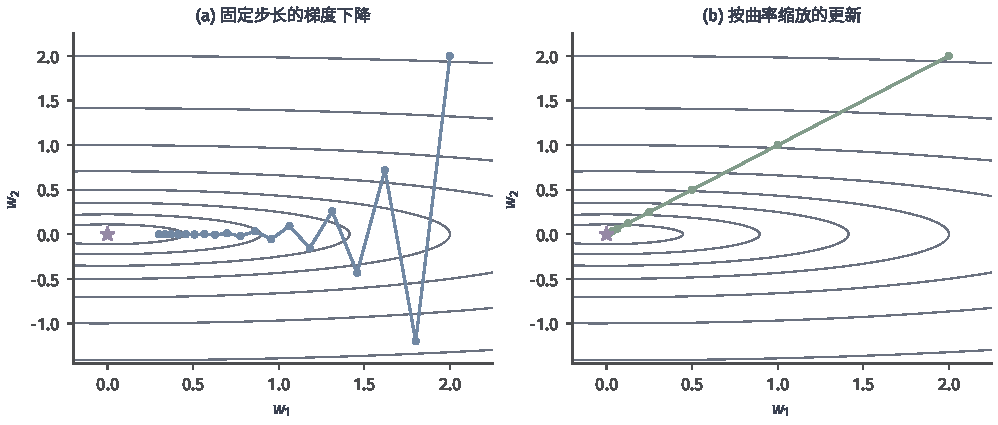
\includegraphics[width=169.0mm]{figures/01-mathematical-preliminaries-upper/01-mathematical-language-combinatorics-analysis-optimization/matplotlib/opt-preconditioned-paths/figure.pdf}
  \caption{例~\ref{ex:opt-anisotropic-preconditioning}中的精确更新路径。灰线是同一二次目标的等值线，蓝、绿圆点分别表示普通更新与预条件更新，星号是最小点。预条件使用了已知曲率，获得和应用这一矩阵的成本仍属于算法代价。}
 \label{fig:opt-preconditioned-paths}
\end{figure*}

这个例子中的预条件恰好消除了两个方向的尺度差。一般目标的曲率会随位置变化，近似矩阵
也有误差；因此图中的直达路径解释机制，不构成所有预条件方法都更快的保证。
从坐标$\bm w=\bm P^{1/2}\bm z$看，预条件只是改变测量方向长度的方式；
它也可以用于牛顿线性方程的迭代求解，并不必然是Hessian的近似逆。
在共同例中，普通$\eta=1/16$梯度法需要
$T\geq\log(2/\varepsilon)/(2\log(16/15))$（并至少一步）达到目标差$\varepsilon$；
对角预条件$\eta=1/2$的目标为$34\,4^{-T}$；
牛顿与Gauss--Newton各解一次对角系统即结束。前两者每步只做向量运算，
而一般稠密二阶方法的矩阵成本不能由这个特殊例子代表。
停止时都应核验原目标或原坐标梯度残差，而不能只看被任意缩小的预条件方向长度。
矩阵分解、条件数与线性方程残差的具体关系可回查第~\ref{chap:matrix-analysis}章。

\section{无约束非光滑目标的求解}
\label{sec:opt-nonsmooth-stochastic-methods}

绝对值损失和稀疏惩罚包含不可微点，普通梯度在那里没有定义。上一节的更新公式在尖点处
直接失去定义，不能靠减小步长绕过，因为问题出在方向本身选不出来。凸性仍能提供支撑目标的
仿射下界，允许用次梯度构造更新；若非光滑项的距离惩罚子问题容易求解，则可以保留原项，
使用邻近映射。前者的每一轮只需一个次梯度，代价低但单步可能上升；后者每轮要解一个子问题，
代价高但能利用不可微点的完整形状。两条路线需要的可计算对象不同。抽样减少信息读取量带来的误差，
在计算预算一节再讨论。

\subsection{基于次梯度的求解}
\label{sec:opt-subgradient-methods}

绝对值损失和$\ell_1$稀疏惩罚在零点不可微，因而不能直接代入普通梯度更新。
问题出在哪？以$f(x)=|x|$为例，$0$左侧的斜率是$-1$、右侧是$+1$，无论把切线斜率
取成哪一个，都只对一侧成立，不存在一个能同时描述两边的“导数”；继续套用
$x\leftarrow x-\eta f'(x)$就无从选择方向。
对凸函数，在可微点处，梯度给出过该点的唯一仿射支撑函数；在不可微点处
这样的支撑直线可能不止一条。把全部支撑直线的斜率收集起来，就得到普通梯度的推广：
它不再是一个方向，而是一组方向，其中每一个都能用于比较函数值。
\begin{definition}[凸次梯度与次微分]
\label{def:opt-convex-subgradient}
设$f:\mathbb R^d\to\mathbb R\cup\{+\infty\}$为适当凸函数，$f(\bm u)$有限。
向量$\bm{g}\in\mathbb R^d$若满足
\[
  f(\bm{v})\geq f(\bm{u})+\langle\bm{g},\bm{v}-\bm{u}\rangle
  \quad\text{对所有 }\bm{v},
\]
就称为$f$在$\bm{u}$处的\term{次梯度}（subgradient）。全部次梯度组成
$\partial f(\bm{u})$，称为次微分；它可以是空集。
\end{definition}
例如
\[
  \partial |x|=
  \begin{cases}
    \{1\},&x>0,\\
    [-1,1],&x=0,\\
    \{-1\},&x<0.
  \end{cases}
\]
凸函数在$\bm{w}^{\star}$处最优，当且仅当
$\bm{0}\in\partial f(\bm{w}^{\star})$。以$f(x)=|x|$为例，零点处
$\partial f(0)=[-1,1]$，零在其中，故$0$是最小点。注意这个判据中“零向量是次梯度”
与“零向量在次微分中”是同一件事，而$\partial f$在不可微点是一整段区间，
因此“存在一个为零的次梯度”比“梯度为零”弱。
若零向量是次梯度，定义立即给出
$f(\bm{v})\geq f(\bm{w}^{\star})$；反过来，若$\bm{w}^{\star}$全局最优，则
$f(\bm{v})\geq f(\bm{w}^{\star})+\langle\bm{0},\bm{v}-\bm{w}^{\star}\rangle$，
所以零向量满足次梯度定义。这个等价性依赖凸次梯度采用全局下界定义。
若要把$f+r$的次微分直接写成$\partial f+\partial r$，或把约束写成指标函数后拆分
次微分，还需限制两个函数的定义域接触方式。
不能只凭两个函数都凸就无条件使用求和等式。本节不依赖这条求和规则，
而直接从支撑不等式推导所需的最优性关系。

次梯度迭代选$\bm g^{(t)}\in\partial f(\bm w^{(t)})$及正步长$\eta^{(t)}>0$，并令
$\bm w^{(t+1)}=\bm w^{(t)}-\eta^{(t)}\bm g^{(t)}$。
支撑斜率提供下界，却未必是实际下降方向。例如$f(x)=|x|$，在$x=0.2$取$\eta=1$，
更新到$-0.8$后目标反而增大，这一次是步长过大的结果。
尖点还可能让任意小步都不能下降：对$f(x,y)=|x|+y/2$，
在$(0,0)$可取次梯度$(1,1/2)$，沿其负方向移动$t>0$后目标为$3t/4>0$。
所以不能给次梯度更新强加光滑梯度的逐步下降要求。实际输出可取已访问点中目标最小者，
或取步长加权平均$\bar{\bm w}^{(T)}=\sum_{t<T}\eta^{(t)}\bm w^{(t)}/\sum_{t<T}\eta^{(t)}$。


图~\ref{fig:vol1-add-subgradient-not-descent}沿刚才选定的负次梯度方向直接比较真实函数值与支撑下界。下界可以下降而真实函数上升，因此支撑不等式本身不能提供逐步下降保证。
\begin{figure}[!htb]
  \centering
  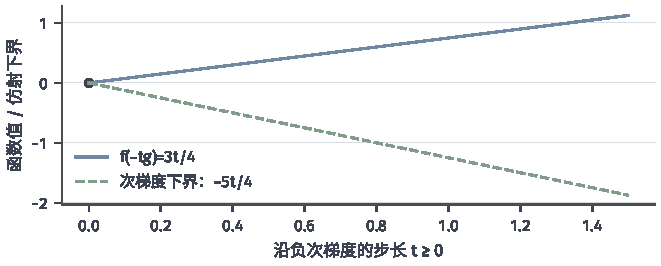
\includegraphics[width=112mm]{figures/01-mathematical-preliminaries-upper/01-mathematical-language-combinatorics-analysis-optimization/matplotlib/comprehension-additions/subgradient-not-descent.pdf}
  \caption{令$f(x,y)=|x|+y/2$，在$(0,0)$选择次梯度$\bm g=(1,1/2)^\top$。沿$-t\bm g$、$t\geq0$移动时，真实函数值为$3t/4$，而该次梯度给出的仿射下界为$-5t/4$。下界始终有效，真实函数却对任意$t>0$上升；两条线由同一解析例子计算。}
  \label{fig:vol1-add-subgradient-not-descent}
\end{figure}

用$f(x,y)=|x|+|y|$可以核对这种差别。在$(0.5,0)$处，$x$方向的支撑斜率只能为$1$，
$y$方向却可取$[-1,1]$中的任意值，因此次微分为$\{1\}\times[-1,1]$。
从中取$(1,0)^\top$，沿其负方向走到$(-0.5,0)$，函数值不变；
在$(0,0)$处可取$(1,1)^\top$，沿其负方向移动$t>0$得到目标值$2t>0$，反而上升。
这些例子排除的是逐步下降的普遍保证；后面可以对加权平均点或历史最佳点建立累计误差界，
而不是要求每个被访问点的目标值都下降。

下面在两项前提下评价误差：次梯度沿迭代有统一范数上界$G$，初值到最小点的距离不超过$R$。
设$f$凸、最小点$\bm w^\star$存在，沿迭代能取得$\|\bm g^{(t)}\|_2\leq G$，
且$\|\bm w^{(0)}-\bm w^\star\|_2\leq R$。展开距离并用次梯度下界得
\[
 \|\bm w^{(t+1)}-\bm w^\star\|_2^2
 \leq\|\bm w^{(t)}-\bm w^\star\|_2^2
 -2\eta^{(t)}(f(\bm w^{(t)})-f^\star)+(\eta^{(t)})^2G^2.
\]
求和消去中间距离，再对平均点用Jensen不等式，得到
\begin{equation}
\begin{aligned}
 \min_{t<T}(f(\bm w^{(t)})-f^\star)
 &\leq\frac{\sum_{t<T}\eta^{(t)}(f(\bm w^{(t)})-f^\star)}{\sum_{t<T}\eta^{(t)}},\\
 f(\bar{\bm w}^{(T)})-f^\star
 &\leq\frac{R^2+G^2\sum_{t<T}(\eta^{(t)})^2}{2\sum_{t<T}\eta^{(t)}}.
\end{aligned}
 \label{eq:opt-subgradient-finite-rate}
\end{equation}
同一右端也控制最佳候选。已知预算$T$且$R,G>0$时，固定
$\eta^{(t)}=R/(G\sqrt T)$给出$RG/\sqrt T$；不知道预算时可用递减步长，把实际使用的
累计步长$\sum_{t<T}\eta^{(t)}$与平方步长和$\sum_{t<T}(\eta^{(t)})^2$代入上式评价误差：
前者是加权平均的总权重，后者乘以$G^2$，给出距离递推中平方更新项的累计上界。
实际路径长度为$\sum_{t<T}\eta^{(t)}\|\bm g^{(t)}\|_2$，还依赖每次次梯度的尺度，
不能由累计步长单独确定。要使误差界趋零，总权重须相对初始距离项与平方步长项持续增大。
例如$\eta^{(t)}=R/(G\sqrt{t+1})$时，前者至少为$\sqrt T$量级，后者只按$\log T$量级增长，
误差界仍以$O(\log T/\sqrt T)$趋零。边界上次微分可能为空，强凸二次目标在全空间的次梯度也未必有界；
上界$G$必须由目标或迭代区域另行保证，不能省略。

凸次梯度依赖全域仿射下界。对于非凸函数，这种下界可能不存在；下一小节改用邻近可微点的信息描述局部驻点。

\subsection{非凸目标的驻点}
\label{sec:analysis-nonsmooth-surrogate-gradient}
\paragraph{一元Clarke广义梯度}

局部Lipschitz一元函数在几乎每个邻近位置有导数，而且这些斜率的绝对值受局部Lipschitz常数控制。因此可以收集邻近可微点趋向当前点时，导数出现的各个极限，再容纳它们的加权平均。非负权重且权重和为一的有限平均称为凸组合；纳入全部凸组合及其极限得到闭凸包。这个过程保留多种局部斜率，不强行选出唯一导数。

\begin{definition}[一维Clarke广义梯度]
\label{def:analysis-clarke-generalized-gradient}
设$U\subseteq\mathbb R$为开集，$f:U\to\mathbb R$局部Lipschitz。对$x\in U$，
$f$在$x$处的\term{Clarke广义梯度}（Clarke generalized gradient）在一维中是如下实数集合：
\[
  \partial^\circ f(x)
  =
  \overline{\operatorname{conv}}
  \left\{
    \lim_{k\to\infty}f'(x_k):
    \begin{array}{l}
      x_k\in U,\quad x_k\to x,\\
      f\text{在每个 }x_k\text{处可导},\\
      \text{且上述导数极限存在}
    \end{array}
  \right\}.
\]
其中$\operatorname{conv}$表示取所有有限凸组合，横线表示在$\mathbb R$中取闭包，
即把集合内序列的所有极限点也纳入。
\end{definition}

同一个斜率集合也可以由移动基点的差商刻画。对实数方向$v$，令
\[
 f^\circ(x;v)=\limsup_{\substack{y\to x\\t\downarrow0}}
 \frac{f(y+tv)-f(y)}t.
\]
这里的联合上极限按邻域中的上确界定义。具体地，先令
\[
 S_\delta=
 \sup_{\substack{|y-x|<\delta,\ 0<t<\delta\\y,\ y+tv\in U}}
 \frac{f(y+tv)-f(y)}t,
\]
再令$\delta\downarrow0$，所得极限就是$f^\circ(x;v)$。
当$\delta$足够小时，局部Lipschitz估计把全部差商的绝对值控制在$L|v|$以内；
邻域缩小时$S_\delta$单调不增，因此这个有限极限存在。
方向$v$的正负区分向右与向左，$|v|$还记录位移尺度。差商不仅从固定$x$出发，还允许起点$y$从附近趋近。对局部Lipschitz一元函数，$\partial^\circ f(x)$恰好由满足$gv\leq f^\circ(x;v)$对所有$v\in\mathbb R$成立的实数$g$组成。于是一个表述收集邻近导数，另一个表述限制移动基点的差商；这两个表述刻画同一个集合。此处陈述等价关系，证明见相关教材\scite{math-clarke1990optimization}。
对连续可微函数，它退化为只含$f'(x)$的单点集；仅在当前点可导时，仍须检查邻近斜率是否稳定，不能一概声称退化为单点。

\paragraph{广义驻点}

在原点，$|x|$邻近可微点的导数为$-1$或$1$，$-|x|$则把这两个斜率的位置交换；两者的Clarke广义梯度都是$[-1,1]$。把$0\in\partial^\circ f(x)$称为广义驻点条件，它本身不能区分极小与极大。局部Lipschitz凸函数的Clarke广义梯度与这项凸次梯度集合一致；对于一般非凸函数，邻近斜率的闭凸包不再保证全域下界。

例如$f(x)=-|x|$在原点左右两侧的导数分别为$1$与$-1$，故其Clarke广义梯度
是$[-1,1]$，包含零；然而原点是局部最大点。若把凸次梯度的全局下界判据用于原点，就要求$-|y|\geq gy$对所有$y$成立。
当$y>0$时，除以$y$得到$g\leq-1$；当$y<0$时，除以负数使不等号反向，得到$g\geq1$。因此不存在满足条件的$g$。
同样的候选区间$[-1,1]$，在$|x|$上可以刻画全局最小点，在$-|x|$上却不提供这样的
保证。这说明广义梯度中含零只是相应的驻点条件，仍要核对所用定义和函数结构。
图~\ref{fig:analysis-clarke-stationarity-boundary}选取两者共有的候选$g=0$。
在$|x|$中，它给出有效的全局下界；在$-|x|$中，原函数反而处处不高于这条线。
局部斜率的凸包抹去了两边斜率出现的次序，不能替代函数整体上下关系。
\begin{figure*}[htbp]
  \centering
  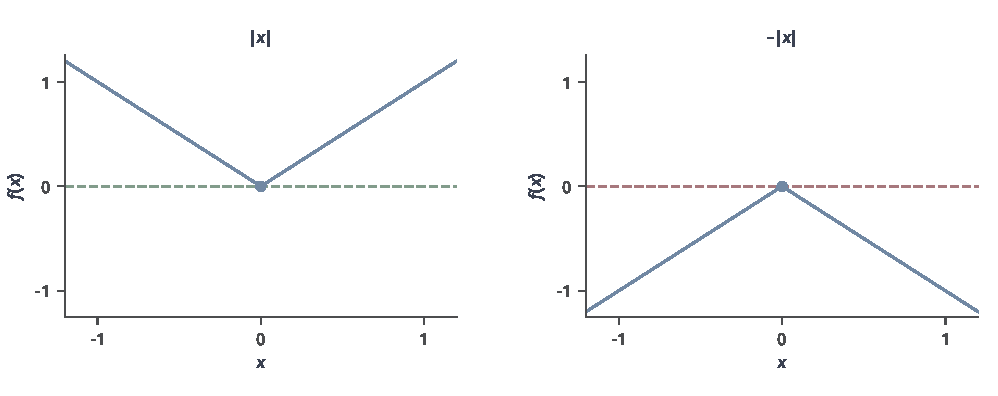
\includegraphics[width=169.0mm]{figures/01-mathematical-preliminaries-upper/01-mathematical-language-combinatorics-analysis-optimization/matplotlib/analysis-clarke-stationarity-boundary/figure.pdf}
  \caption{同一广义驻点条件的不同含义。蓝线分别为$|x|$与$-|x|$，虚线为原点处候选斜率$g=0$对应的直线，左图用绿色，右图用红色。
 两图在原点的Clarke广义梯度均为$[-1,1]$，却分别形成局部最小点与局部最大点；只有左图绿线是全局仿射下界。
 两图共用坐标尺度，由解析式生成。}
 \label{fig:analysis-clarke-stationarity-boundary}
\end{figure*}




\paragraph{多元局部Lipschitz函数}
\label{sec:multivariable-nonsmooth}

一元局部Lipschitz函数几乎处处可导，多元情形也有对应的整体结论。
若开集$U\subseteq\mathbb R^d$上的$f$局部Lipschitz，
即每一点附近都有有限$L$控制$|f(\bm x)-f(\bm y)|\leq L\lVert\bm x-\bm y\rVert_2$，
则Rademacher定理保证$f$关于$d$维勒贝格测度几乎处处全微分存在。
这里的结论是共同线性近似，强于仅声明各偏导数几乎处处存在；
完整证明需要测度估计，不能仅把一元切片上的零测例外相加就得到\scite{math-simon2014geometric}

\paragraph{多元Clarke广义梯度}

这项结论不在例外点指定一个梯度。满足上述局部Lipschitz条件的多元分段仿射函数在各块内部有固定梯度，
接合处则可能有多个邻近梯度极限。对开集$U$上的局部Lipschitz函数$f$，沿用前面一元Clarke广义梯度的构造，可定义
\[
 \partial^\circ f(\bm x)
 =\overline{\operatorname{conv}}\{
 \lim_{k\to\infty}\nabla f(\bm x_k):
 \bm x_k\to\bm x,\ f\text{在}\bm x_k\text{可微，且梯度极限存在}\}.
\]
这里的凸组合是$\sum_{i=1}^r\alpha_i\bm g_i$，其中$\alpha_i\geq0$、$\sum_i\alpha_i=1$；闭凸包收集这些有限组合及其欧氏极限，得到一组候选梯度。
等价地，它由满足$\bm g^\top\bm v\leq f^\circ(\bm x;\bm v)$对所有$\bm v$成立的向量组成，其中
\[
 f^\circ(\bm x;\bm v)
 =\limsup_{\substack{\bm y\to\bm x\\t\downarrow0}}
 \frac{f(\bm y+t\bm v)-f(\bm y)}t.
\]
移动基点的上极限与固定基点方向导数是不同对象。
对$C^1$函数，广义梯度退化为$\{\nabla f(\bm x)\}$；仅在当前点可微还不足以保证这一退化。
对$f(x,y)=|x|$，直线$x=0$上的广义梯度为$[-1,1]\times\{0\}$；
对$- |x|$也得到同一集合，却对应局部最大而非局部最小。
只有在凸性等额外结构下，才能把邻近梯度集合进一步解释为提供全域仿射下界的凸次梯度集合\scite{math-clarke1990optimization}


\subsection{基于邻近映射的求解}
\label{sec:opt-nonsmooth-proximal}
\label{sec:opt-weaker-curvature}

次梯度法允许单步目标上升。在$|x|$的尖点，$[-1,1]$中的每个斜率都给出全局支撑线，
却不是每个负次梯度方向都能下降。换个思路：与其在许多支撑斜率里只挑一个（它未必代表尖点
两侧的全部信息），不如直接把“在尖点附近应该走到哪”当作一个小优化问题来解——
若想让更新读取尖点两侧的整个形状，
可以完整保留难处理的函数项，再加二次距离代价，限制离给定中心$\bm z$的移动。
这就把选一条支撑斜率的更新，改成在“目标小”和“离中心近”之间精确求一个折中点。
两项的作用可以分开看：只用$r$会得到可能远离当前点的最优点，只用距离项则完全不改善目标；
二次距离还带来强凸性，因而折中点总是存在且唯一。$\eta$越大越看重目标下降，越小越接近
原地不动，这正与步长的作用对应。
\begin{definition}[凸函数的邻近算子]
\label{def:opt-proximal-operator}
设$r:\mathbb R^d\to\mathbb R\cup\{+\infty\}$适当、下半连续且凸，$\eta>0$。
函数$r$的\term{邻近算子}（proximal operator）定义为
\[
  \operatorname{prox}_{\eta r}(\bm{z})
  =\argmin_{\bm{w}}
  \left\{r(\bm{w})+\frac{1}{2\eta}
  \lVert\bm{w}-\bm{z}\rVert_2^2\right\}.
\]
\end{definition}
这里的$\eta$只是算子的参数，调节$r$与距离项的相对权重；到后面的邻近点方法和近端梯度中，它才充当步长。二次项使目标强凸。
存在性还需要防止$r$下降得太快，抵消二次距离；下面直接由凸性和下半连续性证明。
后文将“适当、下半连续且凸”简称为“适当闭凸”，这里的“闭”是下半连续性的惯常表述，
不要求有效定义域本身是闭集；对偶部分将再解释这种叫法的几何含义。

\begin{proof}[邻近子问题存在与唯一]
取$\bm u\in\operatorname{dom}r$。下半连续且不取$-\infty$的$r$在紧球
$\{\bm v:\|\bm v-\bm u\|_2\leq1\}$上有有限下界$m$。
否则可取球内$r(\bm v^{(k)})\to-\infty$的序列，再取收敛子列，由下半连续性迫使极限点取$-\infty$。
对$\bm w\in\operatorname{dom}r$且$R=\|\bm w-\bm u\|_2>1$，点
$\bm v=\bm u+(\bm w-\bm u)/R$在该球上，凸性给
\[
 m\leq r(\bm v)\leq(1-1/R)r(\bm u)+r(\bm w)/R,
 \qquad
 r(\bm w)\geq r(\bm u)+R(m-r(\bm u)).
\]
所以$r$的负向增长至多线性；对固定$\bm z$，$\|\bm w-\bm z\|_2^2/(2\eta)$
支配这一线性项。邻近目标强制、下半连续且适当，由存在性小节达到最小值。
其$1/\eta$强凸性又排除两个不同最小点，因而每个$\bm z$都有唯一输出。
\end{proof}

还可以直接取得最优性关系而不预用次微分求和规则。令$\bm p$为邻近最小点，
比较它与$\bm p+t(\bm v-\bm p)$，用$r$的凸性上界并展开平方，除以$t$再令$t\downarrow0$，得
\[
 r(\bm v)\geq r(\bm p)+
 \left\langle\frac{\bm z-\bm p}{\eta},\bm v-\bm p\right\rangle.
\]
故$(\bm z-\bm p)/\eta\in\partial r(\bm p)$；反向将该下界与平方距离相加又可证明最优。
这个关系同时给出邻近解的核验条件。

\begin{theorem}[$\ell_1$邻近算子是软阈值]
\label{thm:opt-soft-threshold}
设$\lambda\geq0$、$\eta>0$。对$r(\bm{w})=\lambda\lVert\bm{w}\rVert_1$，
\[
  [\operatorname{prox}_{\eta r}(\bm{z})]_j
  =\operatorname{sign}(z_j)\max\{|z_j|-\eta\lambda,0\}.
\]
\end{theorem}

\begin{proof}
目标按坐标可分，只需最小化
$\lambda|w|+(w-z)^2/(2\eta)$。若$w>0$，驻点为
$w=z-\eta\lambda$，只在$z>\eta\lambda$时落在该区域；若$w<0$，驻点为
$w=z+\eta\lambda$，只在$z<-\eta\lambda$时有效。若
$|z|\leq\eta\lambda$，零点最优性条件
$0\in\lambda[-1,1]-z/\eta$成立，所以$w=0$。合并三种情形即得结论。
\end{proof}

例如取$\bm z=(3,0.4,-2)^{\top}$与$\eta\lambda=1$，软阈值输出
$(2,0,-1)^{\top}$；小幅坐标被直接置零。若改用
$r(\bm w)=\lambda\lVert\bm w\rVert_2^2/2$，逐坐标驻点给出
$\operatorname{prox}_{\eta r}(\bm z)=\bm z/(1+\eta\lambda)$，在同一参数下为
$(1.5,0.2,-1)^{\top}$。两种正则化都缩小幅度，只有前者在这个例子中产生精确零值。
软阈值中的零区间来自尖点处的一整段可选支撑斜率：当$|z|\leq\eta\lambda$时，
距离项要求的斜率$z/\eta$落在$\lambda[-1,1]$中，零点便能满足子问题最优性条件。
因此，产生精确零值依靠的是完整子问题的平衡，不是给原点任取一个次梯度再走一步。


图~\ref{fig:vol1-add-proximal-balance}直接画出软阈值所求解的子问题。中心较小时，尖点能平衡距离项的斜率，最小点保持在零；中心较大时，平衡点离开零，但仍向尖点方向收缩。
\begin{figure}[!htb]
  \centering
  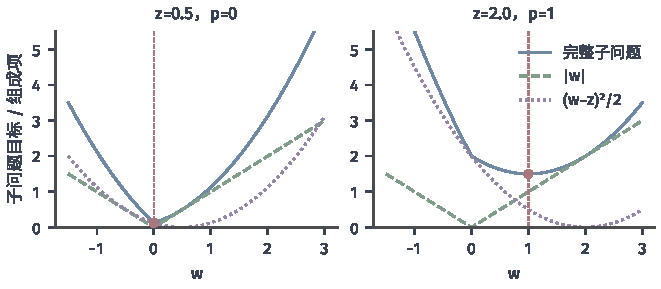
\includegraphics[width=112mm]{figures/01-mathematical-preliminaries-upper/01-mathematical-language-combinatorics-analysis-optimization/matplotlib/comprehension-additions/proximal-balance.pdf}
  \caption{固定$r(w)=|w|$与$\eta=1$，分别取邻近中心$z=0.5,2$。蓝线是完整子问题$|w|+(w-z)^2/2$，绿虚线与紫点线是两项组成；红点为其精确最小点$0,1$。最小化的是两项之和，不能分别最小化后再相加。两面板纵轴尺度相同。}
  \label{fig:vol1-add-proximal-balance}
\end{figure}

邻近算子不会放大输入距离。令
$\bm{p}=\operatorname{prox}_{\eta r}(\bm{x})$、
$\bm{q}=\operatorname{prox}_{\eta r}(\bm{y})$。最优性条件给出
$(\bm{x}-\bm{p})/\eta\in\partial r(\bm{p})$和
$(\bm{y}-\bm{q})/\eta\in\partial r(\bm{q})$。把两个次梯度不等式相加，得到
\[
  \langle\bm{x}-\bm{y},\bm{p}-\bm{q}\rangle
  \geq\lVert\bm{p}-\bm{q}\rVert_2^2.
\]
再用Cauchy--Schwarz不等式便有
$\lVert\bm{p}-\bm{q}\rVert_2\leq\lVert\bm{x}-\bm{y}\rVert_2$。
这个非扩张性质依赖凸次梯度的单调性；非凸邻近子问题可能多解，不能直接沿用。

若能直接求整个目标的邻近解，邻近点方法令
$\bm w^{(t+1)}=\operatorname{prox}_{\eta^{(t)} F}(\bm w^{(t)})$。
与子问题候选$\bm w^{(t)}$比较可得
\[
 F(\bm w^{(t+1)})+\frac{\|\bm w^{(t+1)}-\bm w^{(t)}\|_2^2}{2\eta^{(t)}}
 \leq F(\bm w^{(t)}).
\]
若$F$适当闭凸且有最小点，邻近最优性关系与次梯度下界进一步给出
\[
 2\eta^{(t)}(F(\bm w^{(t+1)})-F^\star)
 \leq\|\bm w^{(t)}-\bm w^\star\|_2^2
 -\|\bm w^{(t+1)}-\bm w^\star\|_2^2
 -\|\bm w^{(t+1)}-\bm w^{(t)}\|_2^2.
\]
固定$\eta>0$时，求和并利用目标单调性得最后一点误差
$F(\bm w^{(T)})-F^\star\leq\|\bm w^{(0)}-\bm w^\star\|_2^2/(2\eta T)$。
这里没有光滑步长限制，但每一步可能需要求解一个几乎同样困难的优化问题；
数学上唯一可解不等于计算上廉价。

对$F=f+r$，若$f$可微且$L$光滑（$L>0$）、$r$适当闭凸，给定步长$\eta>0$，
近端梯度只线性化$f$，将$r$留在子问题中：
\begin{equation}
 \bm w^{(t+1)}
 =\operatorname{prox}_{\eta r}
   \bigl(\bm w^{(t)}-\eta\nabla f(\bm w^{(t)})\bigr).
 \label{eq:opt-proximal-gradient-update}
\end{equation}
一次更新依次计算$\nabla f$、形成邻近中心、求$r$的邻近解，再评价原目标。
例如共同二次目标加$r(\bm w)=\lambda\|\bm w\|_1$时，取$\eta=1/16$，
从$(2,2)$出发先到$(15/8,0)$，随后软阈值得
$(\max\{15/8-\lambda/16,0\},0)$，无需迭代求解邻近子问题。

令$\bm w^+$为该更新、$\bm d=\bm w^+-\bm w$。
邻近最优性给$-\nabla f(\bm w)-\bm d/\eta\in\partial r(\bm w^+)$，
将次梯度不等式用于旧点，再与$f$的光滑上界相加：
\begin{equation}
 F(\bm w^+)\leq F(\bm w)
 -\left(\frac1\eta-\frac L2\right)\|\bm d\|_2^2.
 \label{eq:opt-proximal-gradient-descent}
\end{equation}
故$0<\eta\leq1/L$保证下降。定义可计算的近端梯度映射
\[
 \bm G_\eta(\bm w)=\frac{\bm w-\bm w^+}{\eta}.
\]
它为零当且仅当$0\in\nabla f(\bm w)+\partial r(\bm w)$。
而$\bm G_\eta(\bm w)+\nabla f(\bm w^+)-\nabla f(\bm w)$
属于$\nabla f(\bm w^+)+\partial r(\bm w^+)$，范数至多
$(1+L\eta)\|\bm G_\eta(\bm w)\|_2$，所以这个停止残差确实控制新点的驻点性。
若$F$下有界，固定$\eta\leq1/L$时
$\min_{t<T}\|\bm G_\eta(\bm w^{(t)})\|_2^2
\leq2(F(\bm w^{(0)})-F_{\inf})/(\eta T)$。
非凸$f$下这仍只是驻点保证。

若$f$也凸，任意$\bm v\in\operatorname{dom}r$满足三点不等式
\[
 F(\bm w^+)-F(\bm v)
 \leq\frac{\|\bm w-\bm v\|_2^2-\|\bm w^+-\bm v\|_2^2}{2\eta}
 -\left(\frac1{2\eta}-\frac L2\right)\|\bm w^+-\bm w\|_2^2.
\]
它来自$f$在旧点的凸下界、在新点的光滑上界及$r$在新点的次梯度下界。
取$\bm v=\bm w^\star$、$\eta\leq1/L$并求和，便得
$F(\bm w^{(T)})-F^\star\leq\|\bm w^{(0)}-\bm w^\star\|_2^2/(2\eta T)$。
未知$L$时，可回溯增大二次模型系数直到$f$在新点不超过该模型；
每次试探都需重新求邻近解，其成本应计入预算。

前面的唯一性来自给凸函数补入正二次曲率。如果原目标已经有少量负曲率，
二次距离是否仍能补足它？弱凸性就是对所需补偿量的统一限制。
\begin{definition}[欧氏空间中的弱凸性]
\label{def:opt-weak-convexity}
设$f:\mathbb{R}^d\to\mathbb{R}\cup\{+\infty\}$是适当函数，即不恒为$+\infty$，
且$\rho\geq0$。若
$\bm{w}\mapsto f(\bm{w})+\rho\lVert\bm{w}\rVert_2^2/2$是凸函数，
则称$f$是\term{$\rho$弱凸}（$\rho$-weakly convex）的。取值$+\infty$可以用来表示不可行点。
\end{definition}
若$f$在开凸定义域上二阶可微，这等价于
$\nabla^2f(\bm{w})\succeq-\rho\bm{I}$：负曲率可以存在，但有统一下界。
当$\rho>0$且$0<\eta<1/\rho$时，对任意中心$\bm{z}$，邻近子问题的目标
\[
  f(\bm{w})+\frac{1}{2\eta}\lVert\bm{w}-\bm{z}\rVert_2^2
\]
是$(1/\eta-\rho)$强凸函数；若$\rho=0$，任意$\eta>0$都具有同样的补足曲率作用。
若$f$还下半连续，把$f+\rho\|\cdot\|_2^2/2$代入本节的直接增长证明，
剩余正二次项就保证子问题强制且有唯一解。这正是弱凸性与邻近方法的联系。补入二次曲率
只让这个子问题更易控制，并没有把原函数变成凸函数；弱凸目标仍可有局部极小点和鞍点，
也不保证求得原问题的全局最优解。

例如$f(x)=\cos x$的二阶导数是$-\cos x\geq-1$，所以它是$1$弱凸的，
但仍有无穷多个局部低点。弱凸性限制谷之间最坏的负曲率，并未消除这些谷。
若在当前位置附近加上足够大的二次惩罚，邻近子问题会得到唯一解；改变当前位置后，
所解的却是另一个邻近子问题，不能据此声称原函数只有一个最小点。
前面非凸PL例$f(x,y)=x^2+2\sin^2x$的Hessian下界为$-2\bm I$，
因此它也为$2$弱凸；这只说明两项性质可以共存，不说明任意弱凸函数都满足PL条件。
弱凸邻近映射一般也不再非扩张。例如$f(x)=-\rho x^2/2$且$0<\eta\rho<1$时，
其唯一邻近解为$z/(1-\eta\rho)$，两个输入的距离被放大$1/(1-\eta\rho)$倍。

同一个低维族能显示这些性质各自控制什么。令
\[
  f_a(x_1,x_2)=\frac12(x_1+x_2)^2+\frac{a}{2}(x_1-x_2)^2.
\]
当$a>0$时函数强凸；$a=0$时它凸且满足PL条件，但整条直线$x_1+x_2=0$都是最小点；
$a<0$时函数弱凸却无下界。若限制在紧可行域上，$a<0$时仍有最小点，但驻点
$(0,0)$可能是鞍点。这个例子说明弱凸、PL和强凸不是一条简单的强弱链：弱凸限制最坏负
曲率，PL控制梯度与目标误差，强凸还控制参数距离与唯一性。

\begin{table*}[htbp]
 \centering\small
 \begin{tabularx}{\linewidth}{@{}lXX@{}}
 \toprule
 条件 & 直接控制什么 & 单凭该条件不能得到什么\\
 \midrule
 凸性 & 全部线段上的弦上界；局部最小点也是全局最小点 & 最小点存在、唯一或统一收敛速率\\
 严格凸性 & 非平凡线段上的严格不等式；最小点至多一个 & 一致正曲率下界，例如$x^4$在原点曲率为零\\
 强凸性 & 函数值相对切平面的二次增长（可微情形） & 梯度光滑性，例如$|x|+\mu x^2/2$仍有尖点\\
 弱凸性 & 最坏负曲率的统一下界 & 驻点全局最优或最小点唯一\\
 PL条件 & 梯度大小控制目标值差 & 凸性或参数解的唯一性\\
 \bottomrule
 \end{tabularx}
 \caption{曲率条件的职责比较。各行针对不同性质，不能排成一条从“弱”到“强”的完整等级。}
 \label{tab:opt-curvature-conditions}
\end{table*}

\section{有约束优化的求解}
\label{sec:opt-constraints-duality-certificates}

目标下降的一步可能违反资源约束，因而不能只比较目标值。三种做法的共同问题是“怎样在移动方向上体现约束”：投影法改变的是移动后的落点，每次更新后强制回到可行域；惩罚法改变的是比较准则，把违反量折算进目标，让不可行的点自动变差；乘子法改变的是目标函数本身的结构，为每项约束引入一个待定的系数，并在迭代中同时更新系数与变量。三种做法都要在每步与最终的报告中分别核验原始可行性与目标质量，因为它们各自只保证了
其中一项：投影解总可行但未必改善目标，惩罚解改善折算后的目标但可能不可行，乘子法的
内层解可能既不可行也不最优。下面依次比较三种做法的子问题与停止依据；它们可以结合使用，
但都不能省略这两项核验。

\subsection{基于投影的求解}
\label{sec:opt-projected-methods}

最直接的约束处理方式是不让候选离开可行域：每次沿目标下降方向走一步，若走出了可行域，
就把落点挪到域内离它最近的位置。这一步落在哪，由可行集合的形状决定，与目标无关，
因此可以事先准备。对非空闭凸集$C$，约束指标$\iota_C$适当、下半连续且凸，
其邻近子问题只在$C$内比较平方距离。因此欧氏\term{投影}（projection）
$\Pi_C(\bm{z})=\argmin_{\bm{w}\in C}\lVert\bm{w}-\bm{z}\rVert_2^2$
把一步梯度更新拉回可行域：
\[
  \bm{w}^{(t+1)}
  =\Pi_C\bigl(\bm{w}^{(t)}-\eta^{(t)}\nabla f(\bm{w}^{(t)})\bigr).
\]
这就是取$r=\iota_C$的近端梯度，前面的邻近存在与非扩张证明直接适用。下面把最近点的
几何性质单独写出，后面对分离的证明会回用它。若$C$非凸，最近点可能不存在或不唯一。

\begin{proof}[最近点的直接几何证明]
任取$\bm{x}_0\in C$并令
$R=\lVert\bm{z}-\bm{x}_0\rVert_2$。集合
\[
  C_R=C\cap\{\bm{x}:\lVert\bm{z}-\bm{x}\rVert_2\leq R\}
\]
非空、闭且有界，因而在有限维空间中紧。连续函数
$\lVert\bm{z}-\bm{x}\rVert_2^2$在$C_R$上达到最小值；球外各点到$\bm{z}$的
距离大于$R$，而$\bm{x}_0$的距离等于$R$，所以该最小点也是$C$上的最近点。
若$\bm{p}_1,\bm{p}_2$都是最近点，最近距离为$\delta$，则凸性保证其中点属于$C$，且
\[
  \left\lVert\bm{z}-\frac{\bm{p}_1+\bm{p}_2}{2}\right\rVert_2^2
  =
  \frac12\lVert\bm{z}-\bm{p}_1\rVert_2^2
  +\frac12\lVert\bm{z}-\bm{p}_2\rVert_2^2
  -\frac14\lVert\bm{p}_1-\bm{p}_2\rVert_2^2.
\]
当$\bm{p}_1\neq\bm{p}_2$时，右端严格小于$\delta^2$，与最近距离的定义矛盾，故最近点
唯一，记为$\bm{p}$。

对任意$\bm{x}\in C$，
$\bm{p}+t(\bm{x}-\bm{p})\in C$。函数
$q(t)=\lVert\bm{z}-\bm{p}-t(\bm{x}-\bm{p})\rVert_2^2$在$t=0$
处右导数非负，所以
$\langle\bm{z}-\bm{p},\bm{x}-\bm{p}\rangle\leq0$。
展开$\|\bm z-\bm x\|_2^2$即得
\begin{equation}
 \|\bm p-\bm x\|_2^2+\|\bm z-\bm p\|_2^2\leq\|\bm z-\bm x\|_2^2,
 \qquad \bm x\in C.
 \label{eq:opt-projection-distance}
\end{equation}
\end{proof}


图~\ref{fig:vol1-add-projection-normal}将投影不等式中的两个向量画在同一个起点。从投影点指向外点的向量沿外法向，任一可行弦与它形成直角或钝角，这正对应内积非正。
\begin{figure}[!htb]
  \centering
  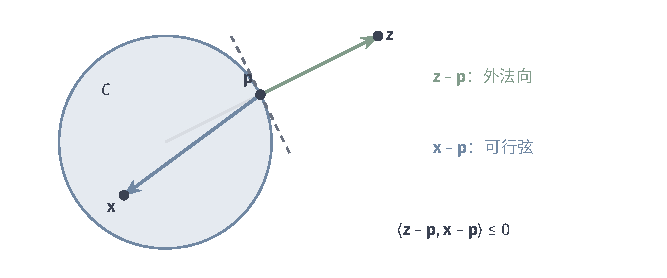
\includegraphics[width=112mm]{figures/01-mathematical-preliminaries-upper/01-mathematical-language-combinatorics-analysis-optimization/tikz/comprehension-additions/projection-normal.pdf}
  \caption{取闭单位圆盘$C$、外点$\bm z=(2,1)^\top$，其投影为$\bm p=\bm z/\|\bm z\|_2$。绿色箭头$\bm z-\bm p$沿外法向，蓝色箭头$\bm x-\bm p$指向一个可行参照点；虚线是支撑切线。内积$\langle\bm z-\bm p,\bm x-\bm p\rangle\leq0$对每个$\bm x\in C$成立，图中只示出其中一条弦。}
  \label{fig:vol1-add-projection-normal}
\end{figure}

这说明投影不增加到任何可行参照点的距离；两个投影输出间的非扩张性则回用邻近证明。
盒约束投影只需逐坐标截断，成本为$O(d)$。
若要求非负坐标之和为$1$，得到概率单纯形（probability simplex）
$\Delta=\{\bm w\in\mathbb R^d:w_j\geq0,\ \sum_jw_j=1\}$。
它的投影具有共同阈值形式
\[
 p_j=\max\{z_j-\tau,0\},\qquad
 \sum_j\max\{z_j-\tau,0\}=1.
\]
阈值同时移动全部坐标，由总和约束确定，不能像盒投影那样完全分开计算。
为核对该形式，对$p_j>0$有$z_j-p_j=\tau$，对$p_j=0$有$z_j\leq\tau$。
故对任意$\bm x\in\Delta$，
$\langle\bm z-\bm p,\bm x-\bm p\rangle
\leq\tau\sum_j(x_j-p_j)=0$；
展开平方距离便知$\bm p$确为最近点。
常用实现先排序以确定哪些坐标为正，再解总和为$1$的阈值；
一般凸集的投影则可能本身就是大型子问题。
在共同二次目标上加范围$C=[1,2]\times[0,2]$，$\eta=0.1$的第一步先到$(1.8,-1.2)$，
再投影为$(1.8,0)$。约束最小点为$(1,0)$，其普通梯度为$(1,0)$而非零；
正确停止量是
$\|\bm w-\Pi_C(\bm w-\eta\nabla f(\bm w))\|_2/\eta$。
它与原始可行性一起检查。若$f$凸且$L$光滑、最小点存在，
前节三点不等式在$\eta\leq1/L$下直接给出目标差$O(1/T)$，
无需为投影另假设普通梯度在边界消失。

图~\ref{fig:opt-proximal-comparison}对同一个标量输入$z$比较三种处理：区间投影把
超出范围的值截到边界；软阈值把小幅值置零、其余幅值减去固定量；二次惩罚则等比例
缩小所有输入。投影保持可行性，软阈值产生稀疏性，二次惩罚改变幅度，它们都可以写成
邻近算子，但输出行为和所解决的问题不同。
\begin{figure}[!htb]
  \centering
  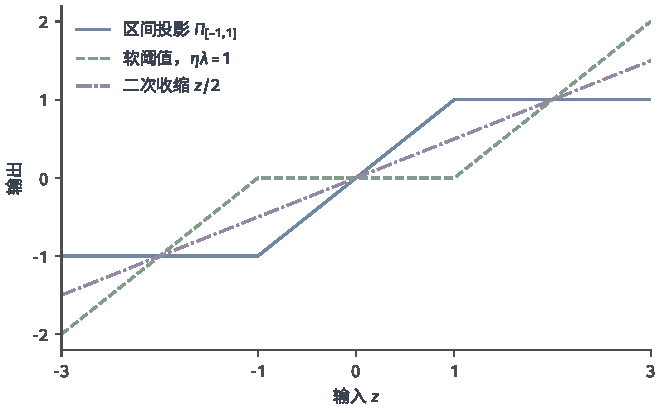
\includegraphics[width=112.0mm]{figures/01-mathematical-preliminaries-upper/01-mathematical-language-combinatorics-analysis-optimization/matplotlib/opt-proximal-comparison/figure.pdf}
  \caption{同一输入$z$的三种邻近映射。投影采用$C=[-1,1]$；软阈值与二次收缩均取$\eta\lambda=1$，分别输出$\operatorname{sign}(z)(|z|-1)_+$和$z/2$。横轴刻度标出阈值位置，曲线由完整分段解析式生成。}
 \label{fig:opt-proximal-comparison}
\end{figure}

\begin{table*}[!htb]
 \centering\small
 \begin{tabularx}{\linewidth}{@{}lXX@{}}
 \toprule
 更新方式 & 每步处理的结构 & 分析前需核对的条件\\
 \midrule
 梯度下降 & 使用可微目标的梯度 & 光滑常数与步长；全局最优保证还依赖凸性或PL等条件\\
 投影梯度 & 梯度更新后求可行集最近点 & 非空闭凸集；投影本身的计算成本\\
 次梯度更新 & 使用非光滑凸目标的全局下界斜率 & 次梯度范数及步长序列；单步目标未必下降\\
 近端梯度 & 光滑部分求梯度，非光滑部分求邻近解 & 光滑部分的步长、正则项的适当闭凸性及可解邻近子问题\\
 \bottomrule
 \end{tabularx}
 \caption{常见一阶更新的结构与条件。相近的更新形式并不共享同一收敛定理。}
 \label{tab:opt-first-order-structures}
\end{table*}

\subsection{基于惩罚的求解}
\label{sec:opt-penalty-methods}

投影可能很贵——一般凸集的投影本身就是一个优化问题；而违反约束的程度常容易计算。
于是可以换一个思路：不强制每次迭代都可行，只把违反量计入目标，让算法自己逐步远离
不可行区域。将约束写为$a_j(\bm w)=0$与$g_k(\bm w)\leq0$后，可将等式残差与不等式正部写成
$V(\bm w)=\sum_j|a_j(\bm w)|+\sum_k[g_k(\bm w)]_+$，
再最小化$f+\rho V$。$V$在约束恰好满足处一般有尖点。若$f$与各约束函数连续可微，
也可以改用平方残差构造二次惩罚$f+\frac\rho2\bigl(\sum_ja_j^2+\sum_k[g_k]_+^2\bigr)$：
$t\mapsto(t_+)^2$的导数$2t_+$连续，所以平方残差连续可微。约束仿射时，平方残差还是
梯度Lipschitz的凸函数；一般非线性约束则要另行核对光滑常数与凸性，例如$a(x)=x^2-1$
光滑，平方后的$(x^2-1)^2$却既不凸，梯度也不全局Lipschitz。
参数$\rho$越大，算法越重视可行性，但两类惩罚的有限参数性质不同。

对共同二次目标加等式$w_1+w_2=1$，二次惩罚问题为
\[
 \min_{\bm w}\frac12(w_1^2+16w_2^2)
 +\frac\rho2(w_1+w_2-1)^2.
\]
解线性驻点方程得
\[
 \bm w_\rho=\frac{(16\rho,\rho)^\top}{16+17\rho},\qquad
 w_{\rho,1}+w_{\rho,2}-1=-\frac{16}{16+17\rho}.
\]
任意有限$\rho>0$下它仍不可行，极限才是约束解$(16/17,1/17)$。
惩罚Hessian为$\operatorname{diag}(1,16)+\rho\bm 1\bm 1^\top$，特征值为
$\bigl(17+2\rho\pm\sqrt{225+4\rho^2}\bigr)/2$。最大特征值随$\rho$无限增大，
固定步长梯度法的稳定上限$2/\lambda_{\max}$因而一直缩小；最小特征值则从$1$增大并趋向$17/2$。
条件数并不单调：$\rho=0$时为$16$，$\rho=1$时约为$8.8$，在$\rho=225/34$处降到最小值约$4.9$，
此后才无限增大。小惩罚先抬高了原来最平坦方向的曲率。在单位法向$(1,1)/\sqrt2$上，
曲率为$17/2+2\rho$；在单位切向$(1,-1)/\sqrt2$上，曲率则恒为$17/2$。
不能只把增大参数看作免费提高精度。


图~\ref{fig:vol1-add-penalty-feasibility-curvature}沿同一罚参数同时核对违反量与最大曲率。残差变小并未使问题自动更容易求解；最大曲率增大，光滑梯度更新可用的固定步长上限随之缩小。
\begin{figure}[!htb]
  \centering
  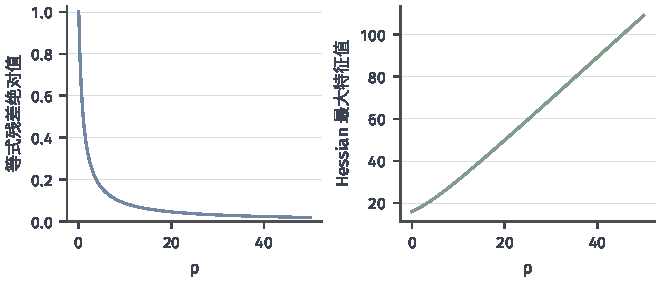
\includegraphics[width=112mm]{figures/01-mathematical-preliminaries-upper/01-mathematical-language-combinatorics-analysis-optimization/matplotlib/comprehension-additions/penalty-feasibility-curvature.pdf}
  \caption{共同二次目标加二次等式惩罚的解析结果，展示$\rho\in[0,50]$。左图为约束违反量$16/(16+17\rho)$，任何有限$\rho$下均非零；右图为惩罚Hessian的最大特征值$(17+2\rho+\sqrt{225+4\rho^2})/2$。两图分别衡量可行性与曲率，不把最大特征值等同于条件数，也不声称条件数单调。}
  \label{fig:vol1-add-penalty-feasibility-curvature}
\end{figure}

一般可行性极限也有前提。设$P\geq0$连续且$P=0$恰好表示可行，
$f$下半连续并在候选区域有统一有限下界$m$，
$\bm w_\rho$精确最小化$f+\rho P$，并存在可行$\bar{\bm w}$。
则$\rho P(\bm w_\rho)\leq f(\bar{\bm w})-m$，所以$\rho\to\infty$时违反量趋零。
若这些解还有有界子列，其极限可行；再与任意可行点比较并使用下半连续性，可知极限全局最优。
没有有界性不能保证存在极限，近似子问题则还要将求解误差加入这个比较。

非平方的惩罚可能在有限参数精确。设比较区域$D$包含所考虑的全部候选及其可行修复，
$f$在$D$上是$K$-Lipschitz的，且每个候选$\bm w\in D$都有可行修复$\bm p\in D$满足
$\|\bm p-\bm w\|_2\leq\kappa V(\bm w)$。由于$\bm w$与$\bm p$都在$D$内，
$f(\bm w)\geq f(\bm p)-K\|\bm p-\bm w\|_2\geq f(\bm p)-K\kappa V(\bm w)$，于是
\[
 f(\bm w)+\rho V(\bm w)
 \geq f(\bm p)+(\rho-K\kappa)V(\bm w).
\]
当$\rho>K\kappa$时，$D$中任何不可行点的惩罚目标都严格大于它的修复点，
因而惩罚问题在$D$上的最优解（若存在）必须可行。
这是一条带明确误差界的精确性条件，不是所有惩罚的共同结论；
后文还将用达到的乘子给出另一种参数对应。

范数约束$\|\bm w\|_1\leq R$规定硬范围；正则项$\lambda\|\bm w\|_1$（$\lambda>0$）则按参数规模计价，
任何非零参数都要付出与其$\ell_1$范数成正比的代价，范数越大代价越高，但它
不直接强制某个预先给定的$R$。含绝对值的惩罚可调用次梯度或邻近方法；
$f$光滑且约束仿射时，二次惩罚可调用光滑方法，一般约束则先按前面的条件核对光滑性。
外层逐步提高$\rho$时，内层既要报告原目标变化，
也要报告约束违反量，不能仅凭惩罚目标的小梯度停机。

同样的区别出现在权重衰减中。普通欧氏梯度下降用于
$f(\bm{w})+\lambda\lVert\bm{w}\rVert_2^2/2$时给出
\[
  \bm{w}^{(t+1)}
  =(1-\eta\lambda)\bm{w}^{(t)}-\eta\nabla f(\bm{w}^{(t)}),
\]
与直接乘上衰减因子相同。若使用预条件矩阵$\bm{P}$，惩罚梯度产生
$-\eta\lambda\bm{P}\bm{w}^{(t)}$，而坐标无关的直接衰减仍为
$-\eta\lambda\bm{w}^{(t)}$；除非$\bm{P}=\bm{I}$或另有匹配，它们不再相同。

\subsection{基于乘子与对偶的求解}
\label{sec:opt-multiplier-dual-methods}

有限惩罚系数由任务设定，并不自动等于最优约束的影响：同一个$\rho$对不同约束的影响
可能差别很大，为了达到足够的精度往往需要反复试算。
这里先建立一个经济学直觉：在最优解处，把某条紧约束的预算放宽一点点，目标能改善多少？
这个“边际价格”不是随便拍的罚权，而是由问题自身决定的；最优解处收紧约束带来的目标增量
恰好与它挂钩。乘子就是把这一价格显式写成变量。乘子把每项约束对目标的作用写成额外
变量，让这个权重本身由问题决定：在最优点处，收紧约束带来的目标增量与乘子挂钩。
前面的惩罚法先固定一个权重再求解，乘子条件则把权重与解一起求出来。
这个平衡可以给出判据，对偶值可以给出最优值的界；要实际求解，还需规定原变量与乘子怎样更新。

\subsubsection{乘子条件与局部最优}
\label{sec:opt-kkt}

资源约束使最优点处的目标梯度不必为零，因为可行方向受到限制。考虑以下问题：
\[
  \min_{\bm{w}}f(\bm{w})
  \quad\text{s.t.}\quad
  a_j(\bm{w})=0\ (j=1,\ldots,m),\quad
  g_k(\bm{w})\leq0\ (k=1,\ldots,p)\text{。}
\]
\begin{definition}[活跃约束与线性化可行方向]
\label{def:opt-linearized-feasible-direction}
设约束函数在可行点$\bm w$处可微。不等式$g_k(\bm w)\leq0$在该点活跃，是指$g_k(\bm w)=0$。
满足
\[
  \langle\nabla a_j(\bm{w}),\bm{d}\rangle=0,\qquad
  \langle\nabla g_k(\bm{w}),\bm{d}\rangle\leq0
  \quad\text{对所有活跃的 }g_k
\]
的方向$\bm{d}$称为\term{一阶可行方向}（linearized feasible direction）。
\end{definition}
这些关系只检验约束的一阶近似，不保证$\bm w+t\bm d$在任意小的正$t$下都可行。
例如约束$x^2\leq0$在$0$处梯度为零，线性化允许任何方向，真实可行点却只有$0$；
后面的资格条件正是为了防止这种一阶信息失真。
等式约束为何产生法向量平衡，可以先看仿射情形
$\bm{A}\bm{w}=\bm{b}$。任一可行扰动都满足$\bm{A}\bm{d}=\bm{0}$；局部最优点
不能沿$\bm{d}$或$-\bm{d}$下降，故
$\langle\nabla f(\bm{w}^{\star}),\bm{d}\rangle=0$对所有
$\bm{d}\in\ker\bm{A}$成立。这里$\ker\bm A=\{\bm d:\bm A\bm d=0\}$，
矩阵乘法逐行读取内积，故$\bm A\bm d=0$恰好要求$\bm d$与每一行向量正交。
把这些行向量的全部线性组合记为$S=\{\bm A^\top\bm y:\bm y\in\mathbb R^m\}$，
就有$\ker\bm A=S^\perp$。有限维欧氏空间中，向量可分为沿子空间与垂直子空间的两部分，
因而$(S^\perp)^\perp=S$；这一正交分解的构造已在第~\ref{sec:ls-orthogonality}节给出。
其中$\operatorname{range}(\bm A^\top)$就是所有$\bm A^\top\bm y$构成的集合$S$。
于是$(\ker\bm{A})^\perp=\operatorname{range}(\bm{A}^{\top})$，存在不受符号限制的
$\bm{\nu}$使
$\nabla f(\bm{w}^{\star})=-\bm{A}^{\top}\bm{\nu}$。
这里的法向量指与所有切向可行扰动垂直的向量；$\bm A$的行给出等式面的法向量。
在共同二次目标加$w_1+w_2=1$的例子中，平衡方程为
$w_1+\nu=0$、$16w_2+\nu=0$和$w_1+w_2=1$，
解出$\nu=-16/17$、$\bm w=(16/17,1/17)^\top$。
等式乘子没有非负限制。这里的负号表示：若将规定总量从$1$稍微增加，最优目标值会增加；它不是不等式预算中的非负资源价格。后面的敏感性公式会把乘子与这一变化率联系起来。


图~\ref{fig:vol1-add-kkt-normal-balance}回到同一个约束二次目标。可行扰动沿直线移动，而非零的目标梯度垂直于这条直线；乘子使两项法向贡献相互抵消，形成驻点平衡。
\begin{figure}[!htb]
  \centering
  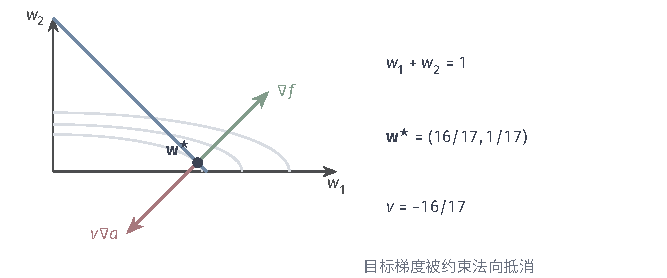
\includegraphics[width=112mm]{figures/01-mathematical-preliminaries-upper/01-mathematical-language-combinatorics-analysis-optimization/tikz/comprehension-additions/kkt-normal-balance.pdf}
  \caption{最小化$(w_1^2+16w_2^2)/2$，约束$a(\bm w)=w_1+w_2-1=0$。蓝线为可行直线，灰线为目标等值线；最优点$\bm w^\star=(16/17,1/17)^\top$处，$\nabla f=(16/17,16/17)^\top$，$\nu=-16/17$给出$\nu\nabla a=-\nabla f$。等式乘子可为负，图中两条等长反向箭头表示相消。}
  \label{fig:vol1-add-kkt-normal-balance}
\end{figure}

活跃不等式只允许切平面一侧的一阶移动，它的外法向量因而以非负系数参与梯度平衡；
不活跃约束在该点留有严格余量，不限制足够小的移动，对应系数应为零。这分别引出
非负乘子与互补松弛。在适当的约束资格条件下，这些几何关系可通过
\term{拉格朗日函数}（Lagrangian）统一表达：
\[
  \mathcal{L}(\bm{w},\bm{\nu},\bm{\alpha})
  =f(\bm{w})+\sum_j\nu_j a_j(\bm{w})
  +\sum_k\alpha_k g_k(\bm{w}),
  \qquad
  \bm{\nu}\in\mathbb{R}^m,\quad
  \bm{\alpha}\in\mathbb{R}_+^p.
\]
在这里，乘子先作为未知系数，把各项约束的梯度并入驻点方程。只有在最优解、乘子与敏感性条件明确以后，才可进一步把它解释为约束变化对最优值的影响。

\begin{definition}[KKT条件]
\label{def:opt-kkt-conditions}
对于上述可微约束问题，候选点$\bm w^\star$与乘子
$\bm\nu^\star\in\mathbb R^m$、$\bm\alpha^\star\in\mathbb R^p$满足
\term{Karush--Kuhn--Tucker条件}（KKT conditions），是指以下四组关系同时成立：
\begin{align}
  \nabla_{\bm{w}}\mathcal{L}(\bm{w}^{\star},\bm{\nu}^{\star},
  \bm{\alpha}^{\star})&=\bm{0},
  &&\text{驻点性},\label{eq:opt-kkt-stationarity}\\
  a_j(\bm{w}^{\star})=0,\quad g_k(\bm{w}^{\star})&\leq0,
  &&\text{原始可行性},\\
  \alpha_k^{\star}&\geq0,
  &&\text{对偶可行性},\\
  \alpha_k^{\star}g_k(\bm{w}^{\star})&=0,
  &&\text{互补松弛}.\label{eq:opt-kkt-complementarity}
\end{align}
等式、不等式约束分别对全部$j=1,\ldots,m$与$k=1,\ldots,p$检验。
\end{definition}
互补松弛逐项连接余量与乘子：若$g_k(\bm w^\star)<0$，对应乘子必须为零；若乘子为正，对应约束必须取等号。取等号仍允许乘子为零，因此活跃约束不能反推出严格正乘子。

四组条件各自对应一条几何或经济含义。驻点性说明目标梯度被约束法向量抵消——在最优点
沿可行方向已经无法继续改善，剩余的一阶变化只能指向离开可行域的方向。原始与对偶可行性
说明候选确实可行、并且价格非负：约束变紧不该让最优值变好。互补松弛说明只有
“卡住”的约束才会标价：留有富余的约束对当前决策没有影响，价格为零；价格严格为正的
约束必然被用到边界。这四条合起来，把“局部最优”翻译成一组可以用代数核验的等式与不等式。

局部最优点满足KKT条件需要\term{约束资格条件}（constraint qualification）。
这里采用一个局部、容易核验的充分条件：$f,a_j,g_k$在点附近连续可微，
全部等式梯度与活跃不等式梯度线性无关，称为线性无关约束资格条件（LICQ）。
它与后面保证凸问题强对偶的Slater条件不是同一个假设。

可借第~\ref{chap:multivariate-calculus}章的隐函数定理直接证明LICQ下的必要性，
无需提前使用后面的分离定理。把等式值、活跃不等式值与适当补充的线性坐标组成
$\bm T(\bm w)=(\bm a(\bm w),\bm g_I(\bm w),\bm z(\bm w))$。
把这些线性无关的梯度行向量扩充为$\mathbb R^d$的一组基，再把新增行作为$\bm z(\bm w)$的系数，
就使$\bm D\bm T=[\bm D\bm a;\bm D\bm g_I;\bm D\bm z]$在当前点可逆。对$\bm T(\bm w)-\bm v=0$，以$\bm w$为待解变量、$\bm v$为参数应用隐函数定理，得到$\bm w$关于$\bm v$的局部连续可微反解，因此$\bm T$在局部给出可逆坐标变换。
未活跃不等式仍严格满足；新坐标中的可行域局部恰为
$\bm a=0,\ \bm g_I\leq0$，而$\bm z$自由。
记新坐标中的目标为$\widetilde f=f\circ\bm T^{-1}$。局部最优时，自由坐标$\bm z$的偏导为零；
活跃不等式坐标只能朝负方向移动，因此对应偏导必须非正，否则沿负方向就能降低目标。
链式法则将这些偏导还原到原坐标：
\[
 \nabla f=(\bm D\bm a)^\top\nabla_{\bm a}\widetilde f
          +(\bm D\bm g_I)^\top\nabla_{\bm g_I}\widetilde f
          +(\bm D\bm z)^\top\nabla_{\bm z}\widetilde f.
\]
最后一项为零。取$\nu_j$为等式坐标偏导的相反数、
$\alpha_k$为活跃不等式坐标偏导的相反数，再令未活跃乘子为零，
链式法则恰给$\nabla f+\sum_j\nu_j\nabla a_j+\sum_k\alpha_k\nabla g_k=0$。
非负性与互补松弛同时成立，这就建立了局部必要性。

没有资格条件，乘子可能不存在。例$f(x)=x$且约束$x^2\leq0$只有可行点
$x=0$，它当然最优；但约束梯度为零，驻点条件$1+\alpha\cdot0=0$无解。

反方向在凸情形更强。若$f$和每个$g_k$均为可微凸函数，$a_j$仿射，且某个可行点与乘子
满足KKT，则对任意可行$\bm{w}$，仿射等式约束使
$\langle\nabla a_j(\bm{w}^{\star}),\bm{w}-\bm{w}^{\star}\rangle
=a_j(\bm{w})-a_j(\bm{w}^{\star})=0$。因此等式乘子项消失，再由凸性和驻点性，
\[
  f(\bm{w})\geq
  f(\bm{w}^{\star})
  -\sum_k\alpha_k^{\star}
  \langle\nabla g_k(\bm{w}^{\star}),\bm{w}-\bm{w}^{\star}\rangle
  \geq f(\bm{w}^{\star}).
\]
最后一步使用凸约束的一阶下界、可行性和互补松弛。因此KKT在该条件下足以保证全局最优。
这个充分性证明不需要LICQ或Slater：只要确实找到满足KKT的候选即可。
反过来，非凸问题即便LICQ成立，KKT也通常只是必要条件；例如无约束$f(x)=-x^2$
在$0$满足驻点条件，却是极大点。
数值计算只能得到近似关系，宜分别报告
$\|\nabla_{\bm w}\mathcal L\|_2$、$\|\bm a\|_2$、$\|[\bm g]_+\|_2$、
$\|[-\bm\alpha]_+\|_2$及$\|\bm\alpha\odot\bm g\|_2$，
其中$\odot$表示逐坐标乘积。小残差不是无条件的目标差证书：
即使无约束凸目标$f(x)=\epsilon x^2/2$，梯度大小$\delta$也对应目标差
$\delta^2/(2\epsilon)$，仍须知道曲率尺度。若已找到精确可行点及可信的对偶下界，
才可直接用二者的差控制全局目标误差。

\begin{example}[活跃约束与乘子]
\label{ex:opt-scalar-active-constraint}
最小化$f(x)=(x-2)^2/2$，约束$x\leq a$。无约束最小点为$2$，因此
$x^\star(a)=\min\{2,a\}$。将约束写成$g(x)=x-a\leq0$，KKT条件为
$x-2+u=0$、$u\geq0$、$x\leq a$与$u(x-a)=0$。
当$a=1$时，$x^\star=1$、$u^\star=1$；当$a=3$时，$x^\star=2$、$u^\star=0$。
约束是否取等号决定乘子能否抵消目标继续下降的梯度。
最优值为$v(a)=(2-a)^2/2$对$a<2$成立，$a\geq2$时为零。
在$a=1$附近，$v'(a)=a-2=-u^\star$：增加一小单位资源上限，最优代价下降的局部速率
由乘子给出。到$a=2$时活跃集改变，解映射的导数由$1$切换为$0$；最优值仍一阶可微，两侧导数都趋于$0$。跨越切换点时，需要分别核对解导数与最优值导数。
\end{example}

\begin{example}[预算约束、活跃集与敏感性]
\label{ex:opt-kkt-budget}
求最接近$\bm{c}=(2,1)^{\top}$的非负分配，并令总预算为$\tau>0$：
\[
  \min_{\bm{w}}\frac12\lVert\bm{w}-\bm{c}\rVert_2^2
  \quad\text{s.t.}\quad
  w_1+w_2\leq\tau,\quad -w_1\leq0,\quad -w_2\leq0.
\]
当$\tau>3$时，$\bm{c}$本身严格满足预算约束，故该约束不活跃，且
$\bm{w}^{\star}(\tau)=(2,1)^{\top}$。当$\tau=3$时解仍为$\bm{c}$，预算约束活跃，
但其乘子为零；这个边界说明“约束活跃”不等于“乘子严格为正”。
当$1<\tau<3$时，两个坐标仍为正而预算取等。把预算这一不等式的乘子记为
$\alpha_{\mathrm{bud}}$，驻点条件给
\[
  w_1-2+\alpha_{\mathrm{bud}}=0,\qquad
  w_2-1+\alpha_{\mathrm{bud}}=0,\qquad
  w_1+w_2=\tau.
\]
因此
\[
  \bm{w}^{\star}(\tau)
  =\left(\frac{\tau+1}{2},\frac{\tau-1}{2}\right)^{\top},
  \qquad
  \alpha_{\mathrm{bud}}^{\star}(\tau)=\frac{3-\tau}{2}.
\]
当$0<\tau<1$时，第二个非负约束也活跃，解变成
$\bm{w}^{\star}(\tau)=(\tau,0)^{\top}$，预算乘子为$2-\tau$，第二个非负约束的
乘子为$1-\tau$。在$\tau=1$处，第二个非负约束活跃但乘子为零。上述区域及边界分别
展示预算不生效、约束活跃但零乘子、仅预算产生正价格，以及预算与坐标边界同时产生
正价格。目标严格凸，满足KKT的点都是唯一全局最优解。
\end{example}

\subsubsection{对偶下界与全局最优}
\label{sec:opt-duality}
\label{sec:opt-affine-certificates}

对固定乘子$\bm{\alpha}\geq\bm{0}$，任意可行$\bm{w}$都满足
$\mathcal{L}(\bm{w},\bm{\nu},\bm{\alpha})\leq f(\bm{w})$。因此
\term{对偶函数}（dual function）
\[
  q(\bm{\nu},\bm{\alpha})
  =\inf_{\bm{w}}\mathcal{L}(\bm{w},\bm{\nu},\bm{\alpha})
\]
给出原问题最优值的下界。我们希望在所有允许的乘子中找到最高的下界，因此定义
\[
 p^\star=\inf_{\bm w:\,\bm a(\bm w)=0,\,\bm g(\bm w)\leq0}f(\bm w),\qquad
 d^\star=\sup_{\bm\nu\in\mathbb R^m,\,\bm\alpha\geq0}q(\bm\nu,\bm\alpha).
\]
这里用下确界和上确界，不预先假定最优点或最优乘子存在。
由构造立即有$d^{\star}\leq p^{\star}$，称为\term{弱对偶}（weak duality）；
两者均有限时，差$p^{\star}-d^{\star}$称为对偶间隙。对某组乘子取下确界得到$-\infty$，表示这组
乘子没有给出有限下界；对偶不可行则表示没有任何乘子满足对偶问题规定的可行条件。前者
描述一个候选乘子的函数值，后者描述整个候选集合，二者不能混用。
若已求得原始可行$\widehat{\bm w}$与有限对偶值$q(\bm\nu,\bm\alpha)$，
则$f(\widehat{\bm w})-q(\bm\nu,\bm\alpha)$是可核验的目标差上界。
具体地，令$U=f(\widehat{\bm w})$、$L=q(\bm\nu,\bm\alpha)$，便有
$L\leq p^\star\leq U$，所以$0\leq U-p^\star\leq U-L$。
可行候选给出上界，对全部原变量取下确界的对偶值给出下界，两者的间隔才成为停止证书。
只改善对偶值还不够：求$q$时选出的内层点可能违反原约束，仍须另找可行候选形成$U$。
要说明这个间隙能否降到零，需要分析目标和约束是否能由仿射界精确描述。
下面按最近点分离、共轭重建、有限生成锥与线性规划的顺序建立这些工具；
每一步都承担不同的证明任务。

\begin{theorem}[闭凸集外一点的严格分离]
\label{thm:opt-projection-separation}
设$C\subseteq\mathbb{R}^d$非空、闭且凸，$\bm{z}\notin C$。则存在
$\bm{a}\neq\bm{0}$和$c\in\mathbb{R}$，使
\[
  \langle\bm{a},\bm{x}\rangle\leq c
  <\langle\bm{a},\bm{z}\rangle
  \quad\text{对所有 }\bm{x}\in C.
\]
\end{theorem}

\begin{proof}
由投影小节的直接证明，$\bm p=\Pi_C(\bm z)$存在且唯一，
并满足$\langle\bm z-\bm p,\bm x-\bm p\rangle\leq0$对所有$\bm x\in C$成立。
取$\bm a=\bm z-\bm p$和$c=\langle\bm a,\bm p\rangle$。由于$\bm z\notin C$，
$\bm a\neq0$，并且
$\langle\bm{a},\bm{x}\rangle\leq c$，而
$\langle\bm{a},\bm{z}\rangle=c+\lVert\bm{a}\rVert_2^2>c$。
\end{proof}

\begin{definition}[支撑超平面与凸锥]
\label{def:opt-supporting-hyperplane-cone}
设$C\subseteq\mathbb R^d$非空，$\bm a\neq0$。若$C$全部位于
$\{\bm x:\langle\bm a,\bm x\rangle\leq c\}$，并且至少有一点取等号，
则等号超平面称为$C$的\term{支撑超平面}（supporting hyperplane）。
非空集合$K$若对所有$\bm u,\bm v\in K$、$\alpha,\beta\geq0$都有
$\alpha\bm u+\beta\bm v\in K$，称为凸锥。
\end{definition}
具体地说，若$\bm{p}$位于闭凸集$C$的边界，可取一列集外点
$\bm{z}^{(k)}\to\bm{p}$，对每个点应用严格分离并把法向量归一化。单位球的紧性给出
收敛子列，极限法向量$\bm{a}\neq\bm{0}$满足
$\langle\bm{a},\bm{x}\rangle\leq\langle\bm{a},\bm{p}\rangle$对所有
$\bm{x}\in C$成立。这说明边界处至少有一个支撑方向，但边界有棱角时法向量未必唯一。
分离把“点不属于集合”转化为一个线性不等式证书，但它本身不自动给出一般凸问题的强对偶；
还需要闭性或约束资格条件。

对称矩阵集合中的\term{半正定锥}（positive semidefinite cone）
\[
  \mathbb{S}_+^d=\{\bm{M}=\bm{M}^{\top}:
  \bm{v}^{\top}\bm{M}\bm{v}\geq0,\ \forall\bm{v}\}
\]
是凸锥，因为非负线性组合仍保持二次型非负。它也是闭集：若
$\bm{M}^{(k)}\to\bm{M}$且每个$\bm{M}^{(k)}\succeq\bm{0}$，则对任意固定
$\bm{v}$都有
$\bm{v}^{\top}\bm{M}\bm{v}
=\lim_k\bm{v}^{\top}\bm{M}^{(k)}\bm{v}\geq0$。
线性规划的非负正交锥和半正定规划的矩阵约束直接定义凸可行域；标准凸二次规划中的
半正定曲率矩阵则保证目标凸。三者共享的是凸目标与凸可行域的语言。若要进一步统一成
带线性目标的锥规划，还需引入辅助变量，用锥约束表达二次目标的界。

分离用仿射函数区分一个点与可行集合。对目标函数，也可以收集所有仿射下界：
固定斜率后找最紧的截距，再比较所有斜率能否重建原函数。凸共轭承担这一步。

上图集$\operatorname{epi}f=\{(\bm x,r)\in\mathbb R^{d+1}:r\geq f(\bm x)\}$
记录图像以上的全部点；它凸与$f$凸等价，闭与$f$下半连续等价。
\begin{definition}[凸共轭与双共轭]
\label{def:opt-conjugate}
给定适当函数$f:\mathbb R^d\to\mathbb R\cup\{+\infty\}$，其\term{凸共轭}
（convex conjugate）定义为
\begin{equation}
 f^*(\bm y)=\sup_{\bm x\in\mathbb R^d}
            \{\langle\bm y,\bm x\rangle-f(\bm x)\},
 \qquad
 f^{**}(\bm x)=\sup_{\bm y\in\mathbb R^d}
            \{\langle\bm y,\bm x\rangle-f^*(\bm y)\}.
 \label{eq:opt-conjugate-biconjugate}
\end{equation}
两个上确界都在整个$\mathbb R^d$上取。$f^*$允许取$+\infty$；若$f^*\equiv+\infty$，
则$f^{**}\equiv-\infty$，否则$f^{**}$不取$-\infty$，但仍可能取$+\infty$。
\end{definition}
这里$f(\bm x)=+\infty$的点不贡献有限共轭候选。固定斜率$\bm y$时，$f^*(\bm y)$是
让$\langle\bm y,\bm x\rangle-f^*(\bm y)$在全域不超过$f$所需的最小截距修正。

\begin{example}[由斜率重建二次函数]
\label{ex:opt-quadratic-conjugate-envelope}
仍取图~\ref{fig:opt-convex-chord-tangent}中的$f(x)=x^2/2$。固定直线斜率$y$，配方得到
\[
 yx-\frac{x^2}{2}
 =\frac{y^2}{2}-\frac{(x-y)^2}{2}.
\]
右边在$x=y$时达到最大值，所以$f^*(y)=y^2/2$。这个共轭值确定了该斜率下最高的
仿射下界
\begin{equation}
 \ell_y(x)=yx-\frac{y^2}{2},\qquad
 f(x)-\ell_y(x)=\frac{(x-y)^2}{2}\geq0.
 \label{eq:opt-quadratic-affine-minorant}
\end{equation}
直线$\ell_y$在$x=y$处与抛物线相切；再提高截距，就会在该点超过$f$。
现在固定输入$x$，让斜率$y$变化。每条直线都在$f$下方，而选择$y=x$就能在这个输入
处达到$f(x)$，因此
\[
 f^{**}(x)=\sup_{y\in\mathbb R}\ell_y(x)=\frac{x^2}{2}.
\]
共轭把函数转换成“每个斜率允许多高的下界”，双共轭则在每个输入处取这些下界中最高的值。
图~\ref{fig:opt-conjugate-affine-envelope}只画三个斜率；它们的逐点最大值是折线，只有
纳入所有实数斜率，才能在每个输入处恢复这条抛物线。
\end{example}

\begin{figure}[htbp]
  \centering
  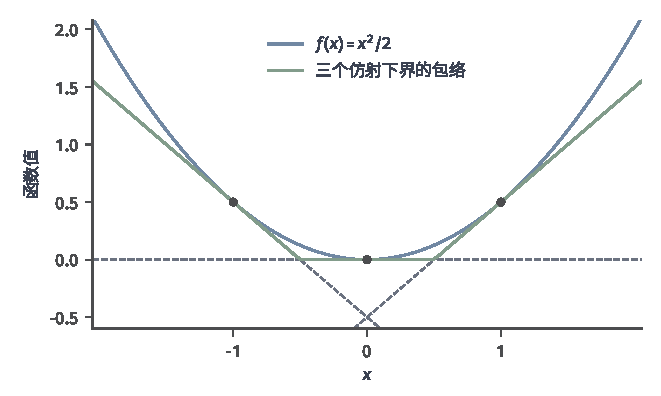
\includegraphics[width=112.0mm]{figures/01-mathematical-preliminaries-upper/01-mathematical-language-combinatorics-analysis-optimization/matplotlib/opt-conjugate-affine-envelope/figure.pdf}
  \caption{$f(x)=x^2/2$与斜率$y=-1,0,1$对应的仿射下界$\ell_y(x)=yx-y^2/2$。
 蓝实线为抛物线，三条灰虚线为下界，绿实线为这三条下界的逐点最大值。
 三个实心点标出相切位置；有限个斜率留下的间隙，在取全部斜率的上确界时消失。
 图为解析教学示例。}
 \label{fig:opt-conjugate-affine-envelope}
\end{figure}

没有任何仿射下界时，这个修正对每个斜率都为无穷。例如$f(x)=-x^2$满足
$f^*(y)=\sup_x\{yx+x^2\}=+\infty$，双共轭因而恒为$-\infty$；适当性本身不能排除这一情形。
由定义立即有\term{Fenchel--Young不等式}
\[
 f(\bm x)+f^*(\bm y)\geq\langle\bm y,\bm x\rangle,
\]
以及$f^{**}\leq f$。共轭是仿射函数族的上确界，因而凸且下半连续；它并非简单把
函数图像交换横纵坐标，也不要求每个上确界都由有限斜率达到。

\begin{theorem}[有限维Fenchel--Moreau定理]
\label{thm:opt-fenchel-moreau}
设$f:\mathbb R^d\to\mathbb R\cup\{+\infty\}$适当、下半连续且凸。
则$f^{**}=f$在全部$\mathbb R^d$上成立，包括$f(\bm x)=+\infty$的点。
因此$f$恰好是全部连续仿射下界的逐点上确界。
\end{theorem}

\begin{proof}
上图集$\operatorname{epi}f=\{(\bm x,r):r\geq f(\bm x)\}$非空、闭且凸。
任取$\bm x_0\in\operatorname{dom}f$及$t_0<f(\bm x_0)$，对上图与其外一点
$(\bm x_0,t_0)$使用定理~\ref{thm:opt-projection-separation}，得到
\[
 \langle\bm a,\bm x_0\rangle+b t_0<c
 \leq\langle\bm a,\bm z\rangle+b r
 \quad\text{对所有 }(\bm z,r)\in\operatorname{epi}f.
\]
上图沿$r$向上无界，故$b\geq0$；若$b=0$，取
$(\bm z,r)=(\bm x_0,f(\bm x_0))$便矛盾，所以$b>0$。
重排得到一个全域仿射下界$\ell_0(\bm z)=\langle\bm p_0,\bm z\rangle-\beta_0\leq f(\bm z)$。
这也保证$f^*(\bm p_0)$有限。

现任取$\bm x$和实数$t<f(\bm x)$，再次严格分离$(\bm x,t)$与上图。
若所得竖直系数$b>0$，立即得到一个仿射下界$\ell$，满足$\ell(\bm x)>t$。
若$b=0$，分离不等式为$\langle\bm a,\bm x\rangle<c\leq\langle\bm a,\bm z\rangle$。
将它与$\varepsilon(r-\ell_0(\bm z))\geq0$相加，得到
\[
 \langle\bm a-\varepsilon\bm p_0,\bm z\rangle+\varepsilon r
 \geq c-\varepsilon\beta_0.
\]
取足够小的$\varepsilon>0$，在$(\bm x,t)$处仍为严格反向不等式，因为原来的分离
间隙为正。新的竖直系数为$\varepsilon>0$，因此仍得到$\ell\leq f$且$\ell(\bm x)>t$。

将这一仿射下界写为$\ell(\bm z)=\langle\bm y,\bm z\rangle-\beta$，有
$f^*(\bm y)\leq\beta$，所以
$f^{**}(\bm x)\geq\langle\bm y,\bm x\rangle-f^*(\bm y)
\geq\ell(\bm x)>t$。
若$f(\bm x)$有限，令$t\uparrow f(\bm x)$；若$f(\bm x)=+\infty$，让$t$任意增大，
两种情形均得$f^{**}(\bm x)\geq f(\bm x)$。结合反向不等式即得结论。
\end{proof}

例~\ref{ex:opt-quadratic-conjugate-envelope}已经用切线族重建了二次函数；定理将这个结论
推广到可能不可微、允许取$+\infty$的闭凸目标。若$f=\iota_{[0,1]}$为闭区间指标函数，
则$f^*(y)=\max\{0,y\}$，双共轭恢复区间内
的零值和区间外的$+\infty$。闭性不能省略：对开区间指标$f=\iota_{(0,1)}$，共轭仍为
$\max\{0,y\}$，但双共轭成为$\iota_{[0,1]}$，在两个端点补上零值。
仿射下界无法区分一个边界点与从内部趋近的极限，下半连续性正是排除这种缺口的条件。

函数等于双共轭也不保证边界处有有限的最优斜率。例如闭凸函数
$f(x)=-\sqrt{x}$对$x\geq0$定义，负半轴取$+\infty$。在$x=0$，有限次梯度$y$若存在，
必须满足$-\sqrt{x}\geq yx$对所有$x>0$成立，即$y\leq-1/\sqrt{x}$，这是不可能的。
$f^{**}(0)=f(0)=0$仍成立，但只能由一列仿射下界逼近，不能声称共轭上确界在某个有限
$y$处达到。由双共轭推导对偶表达时，值相等与最优乘子存在必须分别证明。

共轭也能直接计算对偶下界。例如对单一等式约束问题
$\min_{\bm w}\{f(\bm w):\bm a^\top\bm w=b\}$，固定乘子$\nu$后有
\[
 q(\nu)=\inf_{\bm w}\{f(\bm w)+\nu(\bm a^\top\bm w-b)\}
       =-f^*(-\nu\bm a)-\nu b.
\]
最后一步来自把下确界取负后改写成共轭的上确界，因此不必先求出内层最小点。
若$f(\bm w)=\|\bm w\|_2^2/2$且$\bm a\neq0$，逐坐标配方给$f^*(\bm y)=\|\bm y\|_2^2/2$，
于是$q(\nu)=-\nu^2\|\bm a\|_2^2/2-\nu b$。
它在$\nu^\star=-b/\|\bm a\|_2^2$达到$b^2/(2\|\bm a\|_2^2)$；
原始可行点$\bm w^\star=b\bm a/\|\bm a\|_2^2$也取这个值，故弱对偶就足以认证双方最优。
共轭在这里计算下界，双共轭说明闭凸函数不会在收集全部仿射下界时损失函数值；
但对某个约束问题是否零间隙，仍须像这个例子一样另外核验。

接下来改用有限生成锥研究线性约束的可行性。线性规划的强对偶将由不可行证书推出，
不以双共轭等式代替证明。先建立所需的择一定理
\scite{math-boyd2004convex}

\begin{lemma}[有限生成锥的闭性]
\label{lem:opt-finitely-generated-cone}
给定$\bm{a}_1,\ldots,\bm{a}_r\in\mathbb{R}^m$，集合
\[
  K=\left\{\sum_{i=1}^r\alpha_i\bm{a}_i:\alpha_i\geq0\right\}
\]
是闭凸锥。
\end{lemma}

\begin{proof}
凸性和锥性质由非负线性组合直接得到。为证明闭性，先注意每个$\bm{x}\in K$都能由一组
线性无关的生成向量作非负组合。若某个表示使用的生成向量线性相关，就存在非零系数
$\bm{\gamma}$使$\sum_i\gamma_i\bm{a}_i=\bm{0}$；必要时改变符号，使至少一个
$\gamma_i>0$。从原系数中减去
$t\bm{\gamma}$，其中$t=\min_{\gamma_i>0}\alpha_i/\gamma_i$，仍保持所有系数
非负，并使至少一个系数变为零。重复此过程便得到线性无关的表示。

现取$\bm{x}^{(k)}\in K$且$\bm{x}^{(k)}\to\bm{x}$。线性无关的生成子集只有有限多个，
故可取子列，使每个$\bm{x}^{(k)}$都使用同一个子集$J$。以这些向量为列组成满列秩矩阵
$\bm{A}_J$，相应非负系数满足
\[
  \bm{\alpha}^{(k)}
  =(\bm{A}_J^{\top}\bm{A}_J)^{-1}\bm{A}_J^{\top}\bm{x}^{(k)}
  \longrightarrow
  (\bm{A}_J^{\top}\bm{A}_J)^{-1}\bm{A}_J^{\top}\bm{x}.
\]
极限系数仍逐项非负，且$\bm{x}$等于$\bm{A}_J$乘该极限系数，故$\bm{x}\in K$。
\end{proof}

\begin{lemma}[有限维多面体的线性像]
\label{lem:opt-polyhedral-image}
有限维多面体在线性映射下的像仍是多面体，因而是闭集。
\end{lemma}

\begin{proof}
设多面体$P=\{\bm{u}:\bm{B}\bm{u}\leq\bm{d}\}$，线性映射为
$\bm{v}=\bm{T}\bm{u}$。其图像
\[
  \{(\bm{u},\bm{v}):\bm{B}\bm{u}\leq\bm{d},\
  \bm{v}=\bm{T}\bm{u}\}
\]
是多面体，而$\bm{T}P$是该图像消去$\bm{u}$后的坐标投影。对一个待消变量，
Fourier--Motzkin消元分别收集其系数为正、为负和为零的不等式；每一对正、负系数
不等式消去该变量，零系数不等式原样保留。所得有限组非严格线性不等式恰好描述投影。
逐个消去$\bm{u}$的坐标，便得到$\bm{T}P$的有限线性不等式表示。多面体是有限个闭
半空间的交，因此闭。
\end{proof}

\begin{theorem}[Farkas择一定理]
\label{thm:opt-farkas}
给定$\bm{M}\in\mathbb{R}^{m\times d}$和$\bm{r}\in\mathbb{R}^m$，下列两个系统
恰有一个可行：
\[
  \bm{M}\bm{x}=\bm{r},\quad\bm{x}\geq\bm{0};
  \qquad
  \bm{M}^{\top}\bm{z}\geq\bm{0},\quad
  \bm{r}^{\top}\bm{z}<0.
\]
\end{theorem}

\begin{proof}
两者不能同时成立，因为若都成立，则
$0>\bm{r}^{\top}\bm{z}
=\bm{x}^{\top}\bm{M}^{\top}\bm{z}\geq0$，矛盾。
若第一个系统不可行，$\bm{r}$不属于锥
$K=\{\bm{M}\bm{x}:\bm{x}\geq\bm{0}\}$。它由$\bm{M}$的有限个列向量生成，故由
引理~\ref{lem:opt-finitely-generated-cone}可知$K$是闭凸锥。对$K$与$\bm{r}$应用
定理~\ref{thm:opt-projection-separation}，得到$\bm{a}$和$c$，使
$\langle\bm{a},\bm{k}\rangle\leq c<\langle\bm{a},\bm{r}\rangle$。
由于$\bm{0}\in K$，有$c\geq0$；又因为$t\bm{k}\in K$对所有$t\geq0$成立，
必有$\langle\bm{a},\bm{k}\rangle\leq0$，否则取充分大的$t$便会超过$c$。
令$\bm{z}=-\bm{a}$，可得$\langle\bm{z},\bm{r}\rangle<0$且
$\langle\bm{z},\bm{k}\rangle\geq0$对所有$\bm{k}\in K$成立。特别地，
对$\bm{M}$的每个列向量成立，故
$\bm{M}^{\top}\bm{z}\geq\bm{0}$。第二个系统可行。
\end{proof}

\begin{theorem}[有限维线性规划强对偶]
\label{thm:opt-lp-strong-duality}
考虑标准型原问题与对偶问题
\[
  \min_{\bm{x}\geq\bm{0}}\bm{c}^{\top}\bm{x}
  \quad\text{s.t.}\quad\bm{A}\bm{x}=\bm{b},
  \qquad
  \max_{\bm{y}}\bm{b}^{\top}\bm{y}
  \quad\text{s.t.}\quad\bm{A}^{\top}\bm{y}\leq\bm{c}.
\]
若原问题可行且有限下确界为$p^\star$，则原问题与对偶问题都有最优解，且两个最优值
都等于$p^\star$。
\end{theorem}

\begin{proof}
原始可行域
$P=\{\bm{x}:\bm{A}\bm{x}=\bm{b},\ \bm{x}\geq\bm{0}\}$是非空多面体。由
引理~\ref{lem:opt-polyhedral-image}，其目标值集合
\[
  W=\{\bm{c}^{\top}\bm{x}:\bm{x}\in P\}
\]
是$\mathbb{R}$中的非空多面体。集合$W$下有界，且一维多面体包含自己的有限下端点，
故$p^\star=\inf W$属于$W$。因此存在原始可行点$\bm{x}^{\star}$满足
$\bm{c}^{\top}\bm{x}^{\star}=p^\star$，原问题达到其最优值。

对任意$\varepsilon>0$，系统
\[
  \bm{A}\bm{x}=\bm{b},\quad
  \bm{c}^{\top}\bm{x}+s=p^\star-\varepsilon,\quad
  \bm{x}\geq\bm{0},\ s\geq0
\]
不可行，否则会有目标值小于$p^\star$的原始可行点。对增广矩阵应用
定理~\ref{thm:opt-farkas}，存在$(\bm{y}_{\varepsilon},\gamma_\varepsilon)$满足
\[
  \bm{A}^{\top}\bm{y}_{\varepsilon}
  +\gamma_\varepsilon\bm{c}\geq\bm{0},\quad
  \gamma_\varepsilon\geq0,\quad
  \bm{b}^{\top}\bm{y}_{\varepsilon}
  +\gamma_\varepsilon(p^\star-\varepsilon)<0.
\]
取任一原始可行$\bar{\bm{x}}$并与第一式作内积可知$\gamma_\varepsilon>0$，否则会与
最后一式矛盾。令
$\widehat{\bm{y}}_\varepsilon=-\bm{y}_\varepsilon/\gamma_\varepsilon$，便有
$\bm{A}^{\top}\widehat{\bm{y}}_\varepsilon\leq\bm{c}$且
$\bm{b}^{\top}\widehat{\bm{y}}_\varepsilon>p^\star-\varepsilon$。

记对偶可行多面体为
$D=\{\bm{y}:\bm{A}^{\top}\bm{y}\leq\bm{c}\}$。上面的构造说明$D$非空，且其
目标值集合
\[
  V=\{\bm{b}^{\top}\bm{y}:\bm{y}\in D\}
\]
对每个$\varepsilon>0$都包含一个大于$p^\star-\varepsilon$的值。弱对偶说明$V$中的
每个值都不超过$p^\star$，所以$\sup V=p^\star$。由
引理~\ref{lem:opt-polyhedral-image}，$V$是$\mathbb{R}$中的多面体；非空的一维
多面体只能是闭区间、闭射线、单点或整条实线。由于$V$有有限上确界，它必包含上端点
$p^\star$。因此存在$\bm{y}^{\star}\in D$使
$\bm{b}^{\top}\bm{y}^{\star}=p^\star$，对偶最优解达到与原问题相同的最优值。
\end{proof}

\begin{example}[二维资源分配的原始与对偶证书]
\label{ex:opt-resource-lp-duality}
考虑
\[
  \max_{x_1,x_2\geq0}3x_1+2x_2
  \quad\text{s.t.}\quad
  2x_1+x_2\leq4,\quad x_1+2x_2\leq4.
\]
为两类资源设置价格$u_1,u_2\geq0$。由于原问题是最大化，对可行点的资源余量按非负
价格计价会给出目标上界：
\begin{align*}
  \mathcal{L}(\bm{x},\bm{u})
  &=
  3x_1+2x_2
  +u_1(4-2x_1-x_2)+u_2(4-x_1-2x_2)\\
  &=
  4u_1+4u_2
  +(3-2u_1-u_2)x_1+(2-u_1-2u_2)x_2.
\end{align*}
要使$\sup_{\bm{x}\geq\bm{0}}\mathcal{L}(\bm{x},\bm{u})$有限，$x_1,x_2$的系数
必须非正，因而
$2u_1+u_2\geq3$且$u_1+2u_2\geq2$。此时上确界就是$4u_1+4u_2$，
最小化这个上界得到对偶
\[
  \min_{u_1,u_2\geq0}4u_1+4u_2
  \quad\text{s.t.}\quad
  2u_1+u_2\geq3,\quad u_1+2u_2\geq2.
\]
原始点$(x_1,x_2)=(4/3,4/3)$可行，值为$20/3$；对偶点
$(u_1,u_2)=(4/3,1/3)$可行，值也为$20/3$。弱对偶说明二者同时最优。两项资源约束
和两项产品约束均取等号，互补松弛也逐项成立。
\end{example}

不可行、无界和未达到必须区分。Farkas向量证明约束不可行；若原问题沿可行射线无限改善，
弱对偶只说明不存在给出有限下界的对偶候选，也就是每个允许乘子的对偶函数值都为
$-\infty$，不能据此断言乘子候选集合为空。在线性规划标准型中，这种情形表现为对偶
不可行。若只有下确界而不达到，则不能展示原始最优点。一般凸问题在使用Slater条件前还需
处理低维定义域。沿用定义~\ref{def:opt-proper-domain-indicator}的有效定义域，还需说明低维集合中的“内部”。
\begin{definition}[仿射包与相对内部]
\label{def:opt-affine-hull-relative-interior}
对非空集合$C\subseteq\mathbb R^d$，其\term{仿射包}（affine hull）是全部有限仿射组合
$\sum_i\alpha_i\bm x_i$组成的集合，其中$\bm x_i\in C$、$\sum_i\alpha_i=1$，权重可为负。
点$\bm x\in C$属于\term{相对内部}（relative interior），是指存在$r>0$使
$B(\bm x,r)\cap\operatorname{aff}C\subseteq C$。
\end{definition}

例如平面中的线段没有二维内部，但去掉两个端点后就是它的相对内部。

严格可行点提供了一个不会立即碰到不等式边界的比较位置。下面引用Slater定理的一种有限维版本，
用它判断对偶下界能否达到原最优值。
\begin{theorem}[Slater条件下的强对偶]
设$f$和不等式函数$g_k$都是适当凸函数，即它们不恒为
$+\infty$、从不取$-\infty$且至少在一点取有限值；这些函数具有共同凸定义域$D$，
等式约束为仿射约束$\bm{A}\bm{w}=\bm{b}$。若存在
\[
  \bar{\bm{w}}\in\operatorname{ri}D,\qquad
  \bm{A}\bar{\bm{w}}=\bm{b},\qquad
  g_k(\bar{\bm{w}})<0\quad\text{对所有 }k,
\]
并且原问题最优值有限，则原、对偶最优值相等，且存在最优对偶乘子。
\end{theorem}
共同定义域$D$是这些函数都取有限值的区域。相对内部允许$D$落在低维仿射空间中；
严格不等式要求在这个空间内仍有可行余量。这个条件保证存在有限乘子，足以把最优下界抬到原最优值，
但不保证原始最小点存在。其一般证明需要凸集的一般分离结论，并处理约束值与目标值组成集合的边界；
这类集合未必闭，不能直接套用前面仅针对闭凸集外一点的严格分离定理。
本章不展开这一证明，后面使用时逐项核对这里列出的共同定义域、仿射等式、严格可行点及有限最优值。价值函数与占用度量中的对偶应用
可参考\BookChapterRef{chap:decision-theory-and-dynamic-risk}{卷2《数学准备：概率、因果与决策》第6章“策略的价值与优化”}。

这项结论没有补上原始最小值的达到。例如在实线上最小化$e^x$，没有不等式要违反，
最优值为$0$而没有原始最优点。反过来，某个凸问题即使没有Slater点，
找到KKT候选仍足以证明它全局最优；Slater是用于保证乘子存在和零间隙的充分条件，
不是KKT充分性证明的必需假设。
在预算例~\ref{ex:opt-kkt-budget}中，$\tau>0$时可取足够小的两个正坐标使总和严格小于$\tau$，
因此Slater成立；闭域上的强制目标还保证原始解达到。
于是该例同时具备可行解、原始达到、零间隙和对偶达到。
这四项不能仅凭一个“凸优化问题”名称全部省去核验。

\subsubsection{乘子更新与原始—对偶求解}
\label{sec:opt-multiplier-updates}

KKT是判据，对偶值是证书，它们还没有规定怎样更新未知的乘子。
把乘子合记为$\bm y=(\bm\nu,\bm\alpha)$，允许域为
$Y=\mathbb R^m\times\mathbb R_+^p$。在给定$\bm y^{(t)}$时先求
\[
 \begin{aligned}
 \bm w^{(t)}&\in\argmin_{\bm w}\mathcal L(\bm w,\bm y^{(t)}),\\
 \bm s^{(t)}&=(\bm a(\bm w^{(t)}),\bm g(\bm w^{(t)})),\\
 \bm y^{(t+1)}&=\Pi_Y(\bm y^{(t)}+\eta^{(t)}\bm s^{(t)}).
 \end{aligned}
\]
等式乘子直接加残差，不等式乘子加残差后逐项截到非负区间。
违反预算使价格上升，资源有余量使价格下降；这与原变量沿负梯度更新的方向相反。
内层最小值必须达到且有限，否则这一步没有定义。

为什么残差给出了合法方向？对任意$\bm y'\in Y$，
\[
 q(\bm y')\leq\mathcal L(\bm w^{(t)},\bm y')
 =q(\bm y^{(t)})+\langle\bm s^{(t)},\bm y'-\bm y^{(t)}\rangle.
\]
所以$q$是凹函数，$\bm s^{(t)}$是其全局仿射上界斜率，
$-\bm s^{(t)}\in\partial(-q)(\bm y^{(t)})$。
这正是对凸函数$-q$作投影次梯度下降。
若最优乘子$\bm y^\star$存在、$\|\bm y^{(0)}-\bm y^\star\|_2\leq R_y$，
沿途$\|\bm s^{(t)}\|_2\leq G_y$，投影距离不增和前节距离递推给
\[
 \max_{t<T}q(\bm y^{(t)})\geq
 d^\star-\frac{R_y^2+G_y^2\sum_{t<T}(\eta^{(t)})^2}{2\sum_{t<T}\eta^{(t)}}.
\]
它控制最好的已访问下界，不要求每一轮下界都上升，更不直接控制原始候选的可行性。

若$q$可微且$-q$为$L_q$光滑，其中$L_q>0$，则用
$\bm y^{(t+1)}=\Pi_Y(\bm y^{(t)}+\nabla q(\bm y^{(t)})/L_q)$
可回用投影梯度的$O(1/T)$目标差界。
一个容易核验的充分设定是内层在固定闭凸域上最小化强凸$f$，
所有对偶化约束仿射为$\bm A\bm w-\bm b$，且内层总能达到唯一解。
强凸最优性比较给
$\|\bm w(\bm y)-\bm w(\bm y')\|_2
\leq\|\bm A\|_2\|\bm y-\bm y'\|_2/\mu$，
这个距离界还可证明$q$确实可微。令$\bm h=\bm y'-\bm y$，
分别把$\bm w(\bm y)$、$\bm w(\bm y')$作为另一内层问题的候选，得到
\[
 \langle\bm A\bm w(\bm y')-\bm b,\bm h\rangle
 \leq q(\bm y')-q(\bm y)
 \leq\langle\bm A\bm w(\bm y)-\bm b,\bm h\rangle.
\]
减去右侧线性主项后，余项绝对值至多为
$\|\bm A\|_2\|\bm w(\bm y')-\bm w(\bm y)\|_2\|\bm h\|_2
\leq\|\bm A\|_2^2\|\bm h\|_2^2/\mu$，是比$\|\bm h\|_2$更小的量。
因此$\nabla q(\bm y)=\bm A\bm w(\bm y)-\bm b$，即内层唯一解的约束残差。
当$\bm A\neq0$时可取$L_q=\|\bm A\|_2^2/\mu$；若$\bm A=0$，梯度恒定，可取任意正上界。一般非线性约束或多解内层不能直接套用这个光滑常数。

沿预算例取$\tau=2$，把非负性留在内层可行域，只更新预算乘子$\alpha$。
内层解为
$\bm w(\alpha)=((2-\alpha)_+,(1-\alpha)_+)^\top$。
在$0\leq\alpha\leq1$上，对偶函数为$q(\alpha)=\alpha-\alpha^2$，
残差为$1-2\alpha$。取$\alpha^{(0)}=0$、$\eta=1/4$，则
\[
 \alpha^{(t)}=\frac12(1-2^{-t}),\qquad
 \bm w^{(t)}=\left(\frac32+\frac{2^{-t}}2,\frac12+\frac{2^{-t}}2\right)^\top,
 \qquad q(\alpha^{(t)})=\frac14-\frac{4^{-t}}4.
\]
前三轮乘子为$0,1/4,3/8$，对应内层分配为
$(2,1),(7/4,3/4),(13/8,5/8)$；预算违反量为$1,1/2,1/4$。
对偶值趋近$1/4$时，有限轮的内层候选仍全部超预算。
本例从两个坐标各减去一半预算残差即可修复为$(3/2,1/2)$，
原目标上界$U=1/4$，与已算下界的间隙为$4^{-t}/4$。
修复如此简单依赖本例两个坐标一直为正；一般问题应单独给出投影或其他可行恢复算法。

即使已经得到最优乘子，任意内层最小点也未必是原解。
在例~\ref{ex:opt-resource-lp-duality}的最优资源价格$(4/3,1/3)$处，
两个产品的系数同时为零，Lagrangian对所有非负分配都等于$20/3$；
内层选$(10,10)$会超出原预算，选$(0,0)$虽可行却不是原始最优。
恢复原解还要满足原始约束及互补松弛。对于仿射约束，
步长加权平均的残差等于各轮残差的加权平均，因此平均常有助于恢复；
是否真的可行及目标是否达标，仍须用原问题重新检验。
内层只近似求解时，残差不再给出精确的对偶上界斜率。第~\ref{sec:opt-block-alternating-distribution}节将把内层目标差加入上界和距离递推，说明怎样同时报告近似残差与仍然有效的对偶下界。

\subsubsection{约束变化与解的敏感性}
\label{sec:opt-constraint-sensitivity}

\paragraph{无约束目标的包络导数}

考虑依赖参数$\theta$的无约束目标$q(z,\theta)$。若局部最优解$z^\star(\theta)$位于定义域内部，它满足驻点方程
\[   F(\theta,z)   =   \frac{\partial q}{\partial z}(z,\theta)   =   0. \]
若$q$二阶连续可微，且 $\partial^2q/\partial z^2$在所考察解处非零，隐函数定理给出该驻点的局部唯一分支。这并不自动说明它是全局最优解；还要由曲率或其他结构核对最优性。
\begin{example}[参数二次目标中的解导数与包络导数]
\label{ex:analysis-parametric-quadratic}
对$\theta>-1$，令
\[   q(z,\theta)   =   \frac12(1+\theta)z^2-\theta z. \]
因为$\theta>-1$，配方得到
\[
  q(z,\theta)=\frac{1+\theta}{2}
  \left(z-\frac{\theta}{1+\theta}\right)^2
  -\frac{\theta^2}{2(1+\theta)}.
\]
平方项的系数为正，所以唯一驻点就是全局最小点。驻点方程为
\[   F(\theta,z)=(1+\theta)z-\theta=0. \]
隐式求导给出
\[   \frac{\mathrm{d}z^\star}{\mathrm{d}\theta}   =   -\frac{\partial F/\partial\theta}{\partial F/\partial z}   =   -\frac{z^\star-1}{1+\theta}. \]
直接消元得到
\[   z^\star(\theta)=\frac{\theta}{1+\theta},   \qquad   \frac{\mathrm{d}z^\star}{\mathrm{d}\theta}   =   \frac{1}{(1+\theta)^2}, \]
两种计算一致。

最优值$V(\theta)=q(z^\star(\theta),\theta)$的链式求导为
\[   V'(\theta)   =   \frac{\partial q}{\partial z}   \frac{\mathrm{d}z^\star}{\mathrm{d}\theta}   +   \frac{\partial q}{\partial\theta}. \]
在内部驻点，第一项因$\partial q/\partial z=0$消失，所以
\begin{equation}
  V'(\theta)
  =
  \left.
  \frac{\partial q}{\partial\theta}
  \right|_{z=z^\star(\theta)}
  =
  \frac12(z^\star)^2-z^\star.
\label{eq:analysis-envelope-quadratic}
\end{equation}
另一方面，直接代回可得
\[   V(\theta)=-\frac{\theta^2}{2(1+\theta)},   \qquad   V'(\theta)   =   -\frac{\theta(\theta+2)}{2(1+\theta)^2}, \]
与式~\eqref{eq:analysis-envelope-quadratic}一致。
\end{example}

式~\eqref{eq:analysis-envelope-quadratic}体现了\term{包络定理}
（envelope theorem）的基本机制：最优值的一阶变化不需要显式乘上最优解导数，因为目标对决策变量的一阶导数在内部最优点为零。但解导数本身并未消失；若关心参数变化后 $z^\star$怎样移动，仍要使用隐式求导。边界解、不可微目标、多重最优解或受约束问题需要另外核对条件。下面的预算例子将把约束的变化也纳入最优值导数。


\paragraph{预算约束的敏感性}

预算例~\ref{ex:opt-kkt-budget}也把两类敏感性分开。在$1<\tau<3$时，
$d\bm{w}^{\star}/d\tau=(1/2,1/2)^{\top}$；在$0<\tau<1$时则为
$(1,0)^{\top}$。$\tau=1$处活跃集切换，解连续但导数改变。最优值为
\[
  V(\tau)=
  \begin{cases}
    0, & \tau\geq3,\\
    (3-\tau)^2/4, & 1\leq\tau\leq3,\\
    \bigl((2-\tau)^2+1\bigr)/2, & 0<\tau\leq1.
  \end{cases}
\]
在每个活跃集固定的开区间内，
$V'(\tau)=-\alpha_{\mathrm{bud}}^{\star}(\tau)$：放宽一单位预算带来的
最优值对预算的变化率是预算乘子的相反数，即预算增加$\Delta\tau>0$时，最优值的一阶下降量为$\alpha_{\mathrm{bud}}^\star\Delta\tau$。解导数是向量，乘子给出的是最优值导数，二者不能混用。

图~\ref{fig:opt-budget-active-set}沿同一个预算轴展示解坐标与乘子。$\tau=1$时第二个
坐标开始离开零边界；$\tau=3$时预算继续增加却不再改善目标。两处切换的条件都需要
通过可行性与互补松弛核对，不能只从曲线是否出现折点判断。
\begin{figure*}[htbp]
  \centering
  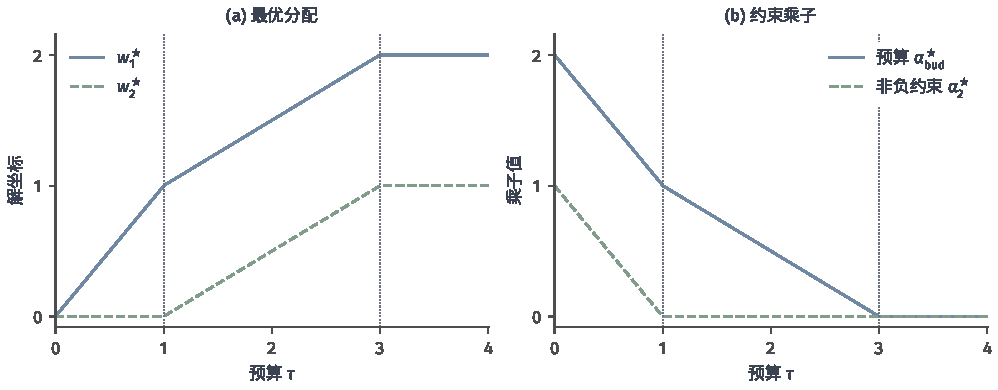
\includegraphics[width=169.0mm]{figures/01-mathematical-preliminaries-upper/01-mathematical-language-combinatorics-analysis-optimization/matplotlib/opt-budget-active-set/figure.pdf}
  \caption{例~\ref{ex:opt-kkt-budget}的解析解。左图为两个最优分配坐标，右图为预算乘子与第二个非负约束的乘子。竖参考线标出$\tau=1,3$；在切换点约束可以取等号而乘子为零，说明活跃性与正价格并不等价。}
 \label{fig:opt-budget-active-set}
\end{figure*}

一般地，设问题依赖参数$\tau$，在一个局部极小点附近固定活跃不等式的指标集$I$。
未活跃乘子恒为零，只把$\bm\alpha_I$作为未知量。将驻点条件、全部等式和活跃不等式的等号条件写成
$\bm\Phi(\bm w,\bm\nu,\bm\alpha_I,\tau)=\bm0$，方程数与未知量数都是$d+m+|I|$。
记这一局部分支为$(\widehat{\bm w},\widehat{\bm\nu},\widehat{\bm\alpha}_I)$。
若$\bm\Phi$连续可微，且对这三组未知量的Jacobian可逆，则第~\ref{chap:multivariate-calculus}章的隐式求导给出
\[
  \frac{d}{d\tau}
  \begin{bmatrix}\widehat{\bm w}\\\widehat{\bm\nu}\\\widehat{\bm\alpha}_I\end{bmatrix}
  =
  -\left(\frac{\partial\bm{\Phi}}
  {\partial(\bm{w},\bm{\nu},\bm{\alpha}_I)}\right)^{-1}
  \frac{\partial\bm{\Phi}}{\partial\tau}.
\]
这个Jacobian是完整KKT系统的导数，原目标Hessian可逆并不足以保证它可逆。活跃集改变或
该矩阵奇异时，解映射可能不可微；此时不能跨越切换点沿用同一个导数。
更具体地，若目标与约束二阶连续可微，记全部等式与活跃不等式的梯度行共同组成$\bm A_I$，并设它满行秩，
则固定活跃集的KKT导数为
\[
 \begin{bmatrix}
 \nabla_{\bm w,\bm w}^2\mathcal L&\bm A_I^\top\\
 \bm A_I&0
 \end{bmatrix}.
\]
若Lagrangian的Hessian在$\ker\bm A_I$上正定，该矩阵可逆：
齐次方程先给$\bm A_I\bm d=0$，与第一行作内积推出$\bm d=0$，
满行秩再迫使乘子增量为零。加上活跃不等式乘子严格为正、未活跃约束有严格余量，
可在小邻域内保持同一活跃集和局部极小分支。
若约束写成$g_k(\bm w)-\tau_k\leq0$而目标不直接依赖$\tau_k$，
定义局部分支值$\widehat V(\bm\tau)=f(\widehat{\bm w}(\bm\tau))$。
对它应用链式法则，并用KKT平衡及活跃约束的导数消去解导数，便得
$\partial\widehat V/\partial\tau_k=-\widehat\alpha_k$，其中未活跃乘子取零。
只有该分支继续为全局最优时，$\widehat V$才等于全局最优值$V$；例如凸问题中满足KKT即可保证这一点。
目标也依赖参数时，还须加入$\partial f/\partial\tau_k$及其余约束的参数项。

惩罚与硬约束有联系，但不是逐参数自动等价。考虑约束问题
\[
  \min_{\bm{w}}f(\bm{w})
  \quad\text{s.t.}\quad
  \lVert\bm{w}\rVert_1\leq R.
\]
若该问题有原始最优解，强对偶成立，并且对偶最优乘子
$\lambda^\star$确实达到，例如满足前述Slater条件且最优值有限，则原始最优解同时最小化
$f(\bm{w})+\lambda^\star\lVert\bm{w}\rVert_1$；Lagrangian中的常数
$-\lambda^\star R$不影响最小点。仅有原、对偶最优值相等并不能保证这样的有限乘子存在。
反过来，不同$\lambda$对应的范数半径可能相同，非凸问题还可能存在对偶间隙。把
$\bm{w}$写成其他参数的函数也会改变优化几何；即使表示同一预测函数，也不保证产生同一
更新轨迹。
反向对应也可以精确说明：若$\widehat{\bm w}$最小化$f+\lambda\|\cdot\|_1$且$\lambda\geq0$，
令$R=\|\widehat{\bm w}\|_1$，则它最小化半径为$R$的约束问题，
因为任何范数不超过$R$且$f$更低的候选都会使惩罚目标更低。
这只构造了与该解匹配的半径，不证明$\lambda$与$R$一一对应。
对一般凸约束，若原始与对偶最优解均达到且对偶间隙为零，取
$\rho>\max\{\|\bm\nu^\star\|_\infty,\|\bm\alpha^\star\|_\infty\}$，
则$f+\rho(\sum_j|a_j|+\sum_k[g_k]_+)$不小于最优Lagrangian，
并对任何非零约束违反多出严格正量。因此有限参数精确惩罚可由达到的乘子支持。
共同二次等式例的$\nu^\star=-16/17$，故$\rho>16/17$的绝对值惩罚已经精确，
与二次惩罚只能在极限可行形成对照。

\section{计算预算有限时的近似优化}
\label{sec:opt-approximate-optimization}

基本更新可以写成一条公式，执行它却需要读取信息、解子问题并重复多轮。若这些成本超过预算，就需要说明简化了什么，以及简化引入的误差如何受控。四种做法回答的是同一个问题——在哪一环上让步：放宽约束改变可行集合；替换每轮目标改变优化对象；拆开变量改变每步的变量范围；近似更新改变梯度或子问题解的信息。让步之后得到的候选仍须按原问题的可行性与误差标准核验，因为每一种简化都只控制被简化后的那个问题。代理目标中将用残差重加权具体构造可核验的上界，近似更新中再说明取整前向与替代反向为什么不自动保留同样的下降保证。

\subsection{基于约束松弛的近似求解}
\label{sec:opt-relaxations-certificates}

离散选择无法直接套用前面的连续方法，因为可行集合没有凸性，梯度信息也无从谈起。
以第~$\ref{chap:combinatorics}$章的选课为例，变量只能取$0$或$1$，目标在这些孤立点上
谈不上斜率，自然无法沿梯度移动。一种做法是把候选集合换成包含它的连续集合，先求出这个较容易问题的解，再设法回到原问题。
第~\ref{chap:combinatorics}章已利用候选范围的包含关系建立松弛界。
现在还需区分两件事：连续集合能否精确包住原候选，以及返回的连续最优点能否恢复为原问题的解。
把原候选的加权平均一并纳入，可以得到包含这些候选的最小凸集。

\begin{definition}[有限点集的凸包]
\label{def:opt-convex-hull}
设$S=\{\bm s_1,\ldots,\bm s_N\}\subseteq\mathbb R^d$非空。
其凸包（convex hull）由这些点的全部凸组合构成：
\[
  \operatorname{conv}(S)
  =\left\{\sum_{i=1}^N\alpha_i\bm s_i:
  \alpha_i\geq0,\ \sum_{i=1}^N\alpha_i=1\right\}.
\]
\end{definition}
例如离散点集
\[
  S=\{(0,0),(1,0),(0,1)\}
\]
可以表示“至多选择一个项目”。把$S$替换为三角形
\[
  \operatorname{conv}(S)
  =\{(x_1,x_2):x_1,x_2\geq0,\ x_1+x_2\leq1\}
\]
得到\term{凸松弛}（convex relaxation）：原来的每个候选仍可行，但增加了分数候选。
对最小化问题，松弛最优值是原最优值的下界；对最大化问题则是上界。

对于有限非空$S$，精确凸包不改变任意线性目标$\bm{c}^{\top}\bm{x}$的最优值：任意
$\bm{x}=\sum_i\alpha_i\bm{s}_i\in\operatorname{conv}(S)$都满足
$\bm{c}^{\top}\bm{x}=\sum_i\alpha_i\bm{c}^{\top}\bm{s}_i
\geq\min_{\bm{s}\in S}\bm{c}^{\top}\bm{s}$，再结合
$S\subseteq\operatorname{conv}(S)$即得最小值相等，最大值同理。
数值相等仍没有指定求解器返回哪个点：若多个候选都最优，它们的凸组合也最优。

\begin{definition}[凸集的极点]
\label{def:opt-extreme-point}
设$K\subseteq\mathbb R^d$为凸集。若$\bm x\in K$满足：对任何$\bm u,\bm v\in K$
与$\theta\in(0,1)$，只要$\bm x=\theta\bm u+(1-\theta)\bm v$，就有
$\bm u=\bm v=\bm x$，则称$\bm x$为$K$的极点（extreme point）。
\end{definition}
极点不能再由其他可行点的非平凡平均得到。线性目标的所有最优点则组成同一个面。
\begin{definition}[线性目标的最优面]
\label{def:opt-optimal-face}
设线性目标$\bm c^\top\bm x$在非空凸集$K$上达到有限最大值$M$。
其最优面（optimal face）为
\[
  K^\star=\{\bm x\in K:\bm c^\top\bm x=M\}.
\]
最小化时，将$M$换为达到的有限最小值即可。
\end{definition}
当$K=\operatorname{conv}(S)$且$S$有限时，最优面正是$S$中全部最优点的凸包：
若一个凸组合对次优点给了正权重，其线性目标值便严格低于最大值。
若$S\subseteq\mathbb Z^d$，最优面还含有整数极点。可以在有限个整数最优点中，
按坐标次序逐项取最大值，选出一个点。若它是两个可行点的非平凡平均，线性最优性先迫使
这两个点都最优，再逐坐标的最大性迫使它们与所选点相同，因此该点确为极点。

即使如此，返回的最优点仍可能是分数点。例如上面的三角形在目标$x_1+x_2$下，
整条边$x_1+x_2=1$都是最优面，$(1/2,1/2)$也最优；逐坐标向上取整却得到
不属于原点集的$(1,1)$。整数极点的存在不保证任意分数最优点都能直接取整。

精确凸包的完整不等式描述可能难以获得。只保留局部约束通常
得到更大的多面体，计算较容易而界更松。若原问题还含乘积$x_ix_j$，可以引入对称矩阵$\bm X$，
用$X_{i,j}$代替这个乘积。精确表达要求$\bm X=\bm x\bm x^\top$，这是非凸的等式。
将它放宽为
\[
 \begin{bmatrix}1&\bm x^\top\\\bm x&\bm X\end{bmatrix}\succeq0
 \quad\Longleftrightarrow\quad \bm X-\bm x\bm x^\top\succeq0
\]
就得到一种半正定松弛。等价性可由二次型配方核对：该块矩阵在$(t,\bm v)$上的值为
$(t+\bm x^\top\bm v)^2+\bm v^\top(\bm X-\bm x\bm x^\top)\bm v$。
精确乘积总满足新约束，但新约束允许$\bm X$与真实乘积有偏差；原来的其他约束也必须保留或相应转换。
新增矩阵有$O(d^2)$个元素，因而它改善界的可能性伴随着更高的存储和锥约束求解成本。

取整还可能破坏约束。考虑
\[
  \max_{x_1,x_2\in\{0,1\}}x_1+x_2
  \quad\text{s.t.}\quad 2x_1+2x_2\leq3.
\]
整数最优值为$1$，而把变量放宽到$[0,1]$后，$(3/4,3/4)$可行且目标值为$3/2$。
逐坐标四舍五入得到$(1,1)$，却违反容量约束；逐坐标向下取整虽可行，却得到目标值$0$。
因此松弛值、恢复可行性的规则和恢复后的目标损失必须分别分析。

若松弛集合比整数可行点的凸包更大，松弛最优值可能严格优于所有整数可行解；
这种最优值差异称为\term{整数间隙}（integrality gap）。上例采用加法差距时，间隙为
$3/2-1=1/2$。更大的松弛不一定产生严格间隙，它还取决于目标；
精确凸包对线性目标没有这种最优值差异，却仍可能包含分数最优点。

图~\ref{fig:opt-hull-relaxation}固定同一个整数问题，把两种连续可行域并列。
精确凸包上的最优值与整数候选一致；局部容量约束定义的松弛多出了整数候选无法平均
得到的区域。这一多出的区域，才使目标上界从$1$升到$3/2$。
\begin{figure*}[htbp]
  \centering
  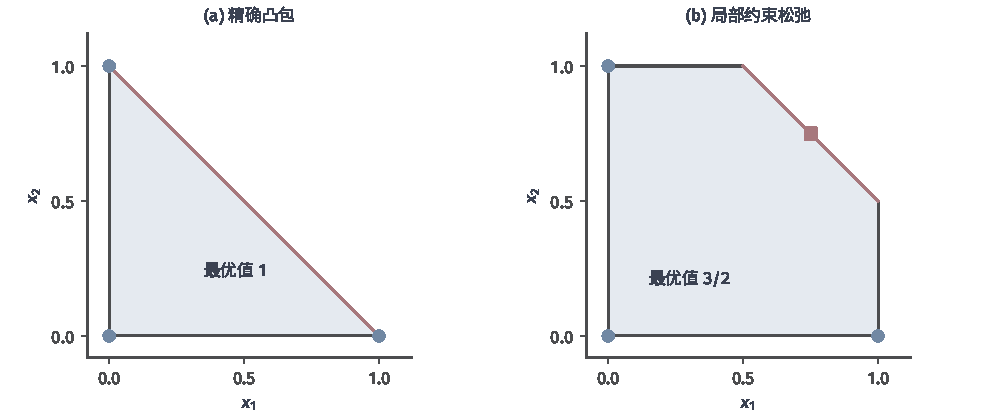
\includegraphics[width=169.0mm]{figures/01-mathematical-preliminaries-upper/01-mathematical-language-combinatorics-analysis-optimization/matplotlib/opt-hull-relaxation/figure.pdf}
  \caption{最大化$x_1+x_2$的两种放宽。左图精确凸包满足$x_1+x_2\leq1$；右图局部松弛满足$0\leq x_i\leq1$与$x_1+x_2\leq3/2$。实心圆为整数可行点，方形为右图的分数最优点$(3/4,3/4)$，粗边标出各自最优面。两图采用相同坐标尺度。}
 \label{fig:opt-hull-relaxation}
\end{figure*}

集合函数的连续扩展也有多种选择。连续变量上的凸性或凹性必须针对所选扩展检验，
不能仅凭原集合函数次模就断言成立；扩展方式决定可用的优化工具。
第~\ref{chap:graph-theory}章会讨论一个可精确求解的特殊情形：二值成对能量满足相应
次模不等式时，可以表示为非负容量的割。一般集合函数的次模性本身，并不保证任意
次模最大化或最小化都能用图割解决。

上面的三角形$\operatorname{conv}(S)$同时说明两件事。原候选$(1,0)\in S$与分数点
$(1/2,1/2)\in\operatorname{conv}(S)\setminus S$在线性目标$x_1+x_2$下都有目标值$1$，
所以这个最优值确实能由原候选取得；但分数点本身不是原问题允许的解。
求解器若返回它，仍需另选或恢复一个属于$S$的最优点。最优数值相同与返回的点原本可行，
是两个不同的保证。

可计算界构成停止证书。对最小化问题，若可行解给出上界$U$，对偶或松弛给出下界$L$，
则
\[
  0\leq U-p^\star\leq U-L.
\]
当$U=L$时已证明全局最优。若把松弛解取整为可行解$\widehat{\bm{x}}$，还应单独分析
$f(\widehat{\bm{x}})-L$；“取整后看起来接近”不是误差界。互补松弛能够证明哪些约束在
最优点活跃的必要关系，却不能仅凭约束活跃就反推正乘子，也不总能直接构造整数解。
图模型中的边缘多面体和MAP松弛会在图与概率对象
建立后复用这里的凸包、上下界和间隙概念。

\subsection{基于代理目标的近似求解}
\label{sec:opt-majorization-improvement}

梯度下降之所以能算出闭式步长，是因为它用一个可计算的二次上界代替了原目标。
这其实是一种“以退为进”：原目标在当前点附近可能形状复杂、没有闭式最优步长，于是先
造一个在当前点与它贴合、但处处盖在它上方的简单函数；把这个简单函数最小化，就能保证
原目标不会变差。若同样的上界来自别的可解结构，这套下降逻辑也能使用，而不要求目标本身是二次函数。
代理函数就是这种用来代替原目标的上界：它必须与目标在当前点取同值、同斜率，并处处不低于目标，
从而保证最小化它不会把原目标推高。
\begin{definition}[主化代理与MM更新]
\label{def:opt-majorization-minimization}
给定目标$F:C\to\mathbb R$、当前点$\bm w^{(t)}\in C$，
\term{主化--最小化方法}（majorization--minimization, MM）在当前点
$\bm{w}^{(t)}$构造代理函数$Q(\bm{w}\mid\bm{w}^{(t)})$，满足
\[
  F(\bm{w})\leq Q(\bm{w}\mid\bm{w}^{(t)}),
  \qquad
  F(\bm{w}^{(t)})=Q(\bm{w}^{(t)}\mid\bm{w}^{(t)}).
\]
上界关系要求对所有$\bm w\in C$成立。若新点$\bm w^{(t+1)}\in C$满足代理值不增，
就称这一步为MM改善更新。
\end{definition}
此时
\begin{align*}
  F(\bm{w}^{(t+1)})
  &\leq Q(\bm{w}^{(t+1)}\mid\bm{w}^{(t)})\\
  &\leq Q(\bm{w}^{(t)}\mid\bm{w}^{(t)})
  =F(\bm{w}^{(t)}).
\end{align*}
第一步用全局上界，第二步用代理改善，最后一步用切触条件。若代理只在当前点附近控制原
目标，而新点走出该邻域，单调链条便会断裂。

下降引理本身给出一个显式代理。若$F$为$L$光滑且$L>0$，可取
\[
  Q(\bm{w}\mid\bm{w}^{(t)})
  =F(\bm{w}^{(t)})
  +\langle\nabla F(\bm{w}^{(t)}),\bm{w}-\bm{w}^{(t)}\rangle
  +\frac{L}{2}\lVert\bm{w}-\bm{w}^{(t)}\rVert_2^2.
\]
它在当前点切触并全局上界$F$。若$C=\mathbb R^d$，精确最小化$Q$恰好得到步长$1/L$的梯度更新；
若$C$是非空闭凸集，配方后得到的是$\Pi_C(\bm w^{(t)}-\nabla F(\bm w^{(t)})/L)$，即投影梯度。仅让代理
与原目标在当前点具有相同梯度，却不满足全局上界，不能推出上面的单调不等式链。

例如$F(x)=x^2/2$、当前点$x^{(t)}=1$，取
$Q(x\mid1)=1/2+(x-1)+(x-1)^2$，则$Q-F=(x-1)^2/2\geq0$且当前点取等号。
代理最小点为$1/2$，于是$F(1/2)=1/8\leq Q(1/2\mid1)=1/4\leq F(1)=1/2$。
图~\ref{fig:opt-majorizer-versus-tangent}把这条链与只有相同局部斜率的切线对照。
\begin{figure}[htbp]
  \centering
  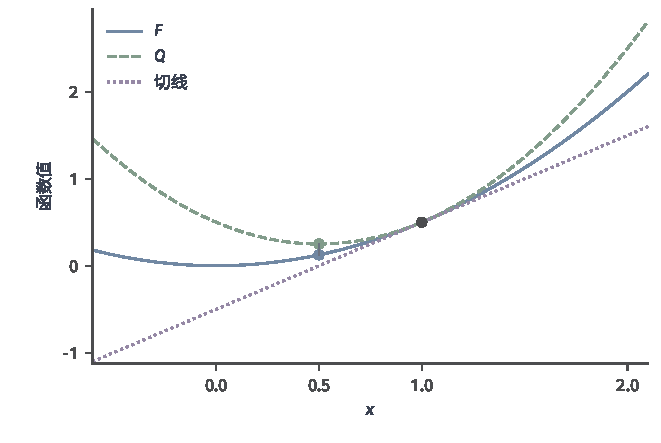
\includegraphics[width=112.0mm]{figures/01-mathematical-preliminaries-upper/01-mathematical-language-combinatorics-analysis-optimization/matplotlib/opt-majorizer-versus-tangent/figure.pdf}
  \caption{代理上界与切线的区别。蓝线为$F(x)=x^2/2$，绿虚线为当前点$1$处的主化代理$Q$，
 紫点线为同点切线$x-1/2$。三者在当前点同值同斜率，但切线位于目标下方，
 最小化它不能使用MM的上界链；绿点标出代理最小点对应的值。图为解析教学示例。}
 \label{fig:opt-majorizer-versus-tangent}
\end{figure}

代理不必精确最小化，但必须分清计算省在何处。记子问题最优值为
\[
 Q^{\star,(t)}=\inf_{\bm w\in C}Q(\bm w\mid\bm w^{(t)}).
\]
若近似子问题解满足
\[
 Q(\bm w^{(t+1)}\mid\bm w^{(t)})\leq Q^{\star,(t)}+\epsilon^{(t)},
\]
则
\[
 \begin{aligned}
 F(\bm w^{(t+1)})&\leq F(\bm w^{(t)})-\Delta^{(t)}+\epsilon^{(t)},\\
 \Delta^{(t)}&=Q(\bm w^{(t)}\mid\bm w^{(t)})-Q^{\star,(t)}\geq0.
 \end{aligned}
\]
只有$\epsilon^{(t)}\leq\Delta^{(t)}$才由此保证本轮原目标不增。实际无需知道$Q^{\star,(t)}$，
也可直接检查新代理值是否低于旧代理值，再决定接受或继续求解。
允许误差超过代理改善时，累计不等式为
$\sum_{t<T}\Delta^{(t)}\leq F(\bm w^{(0)})-\inf_C F+\sum_{t<T}\epsilon^{(t)}$，
其中假设原目标有有限下界。可求和误差控制累计退让，却不自动保证达到全局最优点。

同一数值例中，代理为$Q(x\mid1)=(x-1/2)^2+1/4$。
若只求到$x=3/4$，其代理值为$5/16<1/2$，原目标为$9/32$，仍严格改善；
若返回$x=5/4$，代理误差为$9/16>\Delta^{(t)}=1/4$，原目标反而升为$25/32$。
当任务是最大化$F$时，方向相反：构造切触下界$Q\leq F$，
使$Q(\bm w^{(t+1)}\mid\bm w^{(t)})\geq Q(\bm w^{(t)}\mid\bm w^{(t)})$，
才有$F(\bm w^{(t+1)})\geq Q(\bm w^{(t+1)}\mid\bm w^{(t)})\geq F(\bm w^{(t)})$。
不能沿用最小化的上界方向。

\paragraph{偏大残差下的代价控制}
\label{sec:opt-robust-residual-objectives}

平方代价使残差十的贡献是一的百倍；少量不符合当前模型的读数可能支配拟合。可以保持残差定义，改用增长较慢的损失来控制这种影响。这里研究确定的目标及求解，不由这一改动自动推出统计上的抗污染保证。对可微残差$r_i:\mathbb R^d\to\mathbb R$，写
\[
 F(\bm w)=\tfrac12\sum_i\rho(r_i(\bm w)^2),
 \qquad \rho:[0,\infty)\to\mathbb R.
\]
平方损失对应$\rho(s)=s$。例如取尺度$c>0$，Cauchy损失为$\rho(s)=c^2\log(1+s/c^2)$；Tukey损失在$s\leq c^2$时为$\rho(s)=\tfrac{c^2}{3}[1-(1-s/c^2)^3]$，其后恒为$c^2/3$\scite{math-ceres-loss}。$c$与残差使用相同单位，改变它就改变了开始压低贡献的尺度。

对单项$\rho(r^2)/2$求导，得到相对残差的斜率$r\rho'(r^2)$。平方损失的斜率是$r$；Cauchy为$r/(1+r^2/c^2)$，Tukey为$r(1-r^2/c^2)^2\mathbb I\{|r|\leq c\}$。后两者的斜率在残差很大时趋零或变为零，表示沿残差方向的边际代价减弱。实际参数梯度还要乘$\nabla r_i(\bm w)$，所以对参数更新的作用也取决于残差的Jacobian，不能仅由残差大小判断。代价也变为非凸：仅有驻点不足以判断最优，初始化和尺度选择仍会改变结果。

\paragraph{二次代理下的残差重加权}
\label{sec:opt-irls}

这些损失仍可利用平方残差子问题。假设$\rho$可微、非减且关于$s$凹；凹函数位于切线下方，故$\rho(s)\leq\rho(s_0)+\rho'(s_0)(s-s_0)$。在当前点令$s_i^{(t)}=r_i(\bm w^{(t)})^2$，得到MM上界
\begin{equation}
 Q(\bm w\mid\bm w^{(t)})
 =\mathrm{const}^{(t)}+\tfrac12\sum_i a_i^{(t)}r_i(\bm w)^2,
 \qquad a_i^{(t)}=\rho'(s_i^{(t)})\geq0.
 \label{eq:opt-irls-majorizer}
\end{equation}
每轮先按现有残差算权重，再保持权重不变求加权平方残差，最后重算残差和权重，这就是\term{迭代重加权最小二乘}（iteratively reweighted least squares, IRLS）。Cauchy权重为$(1+s_i^{(t)}/c^2)^{-1}$，Tukey权重为$(1-s_i^{(t)}/c^2)^2\mathbb I\{s_i^{(t)}\leq c^2\}$。它们来自同一目标的切线，不能任意重设权重后仍声称在优化原目标。

若$r_i(\bm w)=\bm x_i^\top\bm w-y_i$，这是线性加权最小二乘。若残差非线性，代理仍是非线性最小二乘，可以在内部使用前面的Gauss--Newton或阻尼更新。仅解一次线性化方程不必改善这个代理；应核验完整加权残差值确实不增，才可使用MM链推出原目标不增。目标下降与参数收敛、全局最优仍是不同结论。

例如用常数$w$拟合读数$0,0,10$，普通平方损失的解是$10/3$。取Cauchy损失、$c=1$并从$w^{(0)}=0$开始，三项权重为$1,1,1/101$；精确最小化代理给出$w^{(1)}=10/203$。偏大读数的作用被减小，这是所选目标及当前残差共同决定的结果，不能据此保证任意污染都能剔除。Tukey还可能让全部权重为零，此时代理为常数、没有可用于确定参数的信息，需要重新检查初始化或尺度。若再加永久正则项，应将同一正则项原样纳入每轮代理，不能与内部控制步长的阻尼混为一项。


\subsection{基于分块更新的近似求解}
\label{sec:opt-block-alternating-distribution}

若变量自然分成$\bm{u}$与$\bm{v}$两组，可以固定一组更新另一组。设$\bm u\in\mathbb R^p$、$\bm v\in\mathbb R^q$，$\bm X\in\mathbb R^{n\times p}$、$\bm Z\in\mathbb R^{n\times q}$、$\bm y\in\mathbb R^n$，$r$与$s$分别为两组变量的惩罚函数。对
\[
  \Phi(\bm{u},\bm{v})
  =\frac12\lVert\bm{X}\bm{u}+\bm{Z}\bm{v}-\bm{y}\rVert_2^2
  +r(\bm{u})+s(\bm{v}),
\]
\term{分块坐标法}（block coordinate method）每次只对一个块走梯度或近端步；
\term{交替最小化}（alternating minimization）则精确或近似求解每个块的条件子问题。
若每次子问题确实降低同一个
$\Phi$，目标值单调不增。精确交替最小化时，这一点直接来自
\[
  \Phi(\bm{u}^{(t+1)},\bm{v}^{(t)})
  \leq\Phi(\bm{u}^{(t)},\bm{v}^{(t)}),\qquad
  \Phi(\bm{u}^{(t+1)},\bm{v}^{(t+1)})
  \leq\Phi(\bm{u}^{(t+1)},\bm{v}^{(t)}).
\]
但非凸情形下仍可能停在局部解或依赖初始化。

一个可复核的耦合二次例子是
\[
  \Phi(u,v)=\frac12(u-v)^2+\frac12(u-1)^2.
\]
固定$v$时的唯一最优点为$u=(v+1)/2$，固定$u$时的唯一最优点为$v=u$。从
$v^{(0)}$出发，一轮交替更新得到
$u^{(t+1)}=(v^{(t)}+1)/2$、$v^{(t+1)}=u^{(t+1)}$，因而
$v^{(t+1)}-1=(v^{(t)}-1)/2$，最终到达联合最优点$(1,1)$。这里的收敛来自这个
正定二次目标的特殊结构。换成非凸目标$(uv-1)^2$并从$(0,0)$开始时，逐块目标在一块
固定为零时没有提供离开零点的理由；若平局规则继续选择零，目标保持为$1$，而全局最优值
为$0$。所以逐块精确和目标单调都不单独保证全局最优。
若无约束目标连续可微，一个点对每一块都已精确最优，则各块偏导同时为零，故它是驻点。
目标联合凸时，这又足以推出全局最优；仅对各块分别凸则不够。
上述$(uv-1)^2$在另一块固定时都是凸二次函数，仍给出了失败例。
对于实际迭代，还须证明它确实收敛到块最优点，而非仅看到目标值收敛。

约束耦合时，可以复制共享变量，再通过一致性约束分解为局部子问题。乘子负责协调副本，
这改变了每步计算位置，却没有删除原约束。若局部问题没有被足够准确地求解，或协调步长
不满足条件，分解形式本身不保证收敛。
具体地，最小化$r(\bm w)+s(\bm w)$可改写为
$\min_{\bm u=\bm v}\{r(\bm u)+s(\bm v)\}$。固定等式乘子$\bm\nu$后，
两项Lagrangian子问题可独立求解：
\begin{align}
 \bm u^{(t)}&\in\argmin_{\bm u}\{r(\bm u)+\langle\bm\nu^{(t)},\bm u\rangle\},\nonumber\\
 \bm v^{(t)}&\in\argmin_{\bm v}\{s(\bm v)-\langle\bm\nu^{(t)},\bm v\rangle\},\nonumber\\
 \bm\nu^{(t+1)}&=\bm\nu^{(t)}+\eta^{(t)}(\bm u^{(t)}-\bm v^{(t)}).
 \label{eq:opt-consensus-dual-decomposition}
\end{align}
输入是两个可分函数及当前价格，子问题输出各自副本，协调量是副本差。
与前一节的交替最小化不同，局部副本可以暂时不一致，所改进的是对偶下界，
因此原始目标并不保证每轮下降；这是使用分解时最容易误解的一点。若两个子问题适当闭凸且强凸，解总存在，
负对偶函数的光滑常数可取$1/\mu_r+1/\mu_s$，步长据此选择；
仅凸时则回用有界残差的对偶次梯度分析。子问题无下界时，这种分解不能直接执行。

取$r(u)=(u-1)^2/2$、$s(v)=(v+1)^2/2$，
内层解是$u=1-\nu$、$v=\nu-1$，对偶函数$q(\nu)=2\nu-\nu^2$。
令$\nu^{(0)}=0$、$\eta^{(t)}=1/4$，得到
$\nu^{(t)}=1-2^{-t}$、$u^{(t)}=2^{-t}$、$v^{(t)}=-2^{-t}$。
第一轮两个副本各自使局部目标为零，却相差$2$；第三次取值为$1/4,-1/4$，
差缩小到$1/2$。将二者平均为共同变量$w=0$，恢复可行上界$r(0)+s(0)=1$，
与$q(\nu^{(t)})=1-4^{-t}$之间的差为$4^{-t}$。
这里的平均恰好最优来自对称二次结构，不是一般副本问题的免费恢复规则。

若每轮只保证
$\mathcal L(\widetilde{\bm w}^{(t)},\bm y^{(t)})\leq q(\bm y^{(t)})+\epsilon^{(t)}$，
将该候选代入另一组乘子会给
\[
 q(\bm y')\leq q(\bm y^{(t)})
 +\langle\widetilde{\bm s}^{(t)},\bm y'-\bm y^{(t)}\rangle+\epsilon^{(t)}.
\]
于是投影次梯度的单步距离界多出$2\eta^{(t)}\epsilon^{(t)}$。累加后，
有限步界的分子应增加
\[
 2\sum_{t<T}\eta^{(t)}\epsilon^{(t)}.
\]
近似内层值本身大于等于$q$，不能直接冒充原问题下界。有可信子问题误差界时，
可用下界为
\[
 \mathcal L(\widetilde{\bm w}^{(t)},\bm y^{(t)})-\epsilon^{(t)}.
\]

变量也可以是一个分布$q$。此时“更新分布”仍是在某个可行分布集合上降低同一目标，而非
一种脱离优化的概率操作。在有限支持$\{1,\ldots,m\}$上，分布变量就是概率单纯形
\[
  \bm{\Delta}_m
  =\{\bm{q}\in\mathbb{R}^m:q_i\geq0,\ \sum_{i=1}^m q_i=1\}.
\]
归一化、非负性和支持集都是可行约束，更新后必须仍留在这个单纯形中。
例如块子问题$\min_{\bm q\in\bm\Delta_2}\|\bm q-(0.8,0.4)^\top\|_2^2/2$
的解不是原向量：为使两坐标和为$1$，各减去$0.1$，得到$(0.7,0.3)^\top$；
非负性仍成立，因此它满足该凸投影问题的最优性条件。
EM与变分方法还需要
期望、条件分布和散度，相关对象可参考\BookChapterRef{chap:random-variables}{卷2《数学准备：概率、因果与决策》的“随机变量与概率基础”章}和
\BookChapterRef{chap:information-theory-and-statistical-geometry}{卷2《数学准备：概率、因果与决策》的“概率分布的分析与优化”章}。
这些方法将复用交替优化与MM的单调性核对方式。

\subsection{基于近似更新的求解}
\label{sec:opt-stochastic-gradient-stability}

有限和目标
\[
  F_S(\bm{w})=\frac1n\sum_{i=1}^n\ell_i(\bm{w})
  +\frac{\lambda}{2}\lVert\bm{w}\rVert_2^2
\]
的经验损失梯度要读取全部$n$项。这里的抽取先只用有限概率权重理解，$\mathbb E_I$表示按这些权重求和。
随机迭代的收敛还需要步长、累计噪声与平均动力学条件，可参考
\BookChapterRef{chap:action-and-state}{卷2《数学准备：概率、因果与决策》第4章“动力系统”}。
若$I$在$\{1,\ldots,n\}$上均匀抽取，则完整目标的
随机梯度可取
\[
  \bm{g}_I(\bm{w})
  =\nabla\ell_I(\bm{w})+\lambda\bm{w},\qquad
  \mathbb{E}_I[\bm{g}_I(\bm{w})]
  =\nabla F_S(\bm{w}).
\]
若按概率$p_i>0$非均匀抽取，则应改用
\[
  \bm{g}_I(\bm{w})
  =\frac{\nabla\ell_I(\bm{w})}{np_I}+\lambda\bm{w}.
\]
正则项梯度$\lambda\bm{w}$是确定量，无需抽样；小批量只需平均若干经过相应加权的
损失梯度，再加上这项确定梯度。
例如$n=2$、当前位置两项标量梯度为$2,-1$，完整损失梯度为$1/2$。
若以$p_1=3/4,p_2=1/4$抽样而不重加权，均值为$5/4$，已经改变更新方向的大小；
使用$1/(np_I)$后，两种输出为$4/3,-2$，均值恢复为$1/2$。

在第$t$轮固定已经得到的历史和当前点，再按该轮概率求有限加权平均，记作$\mathbb E^{(t)}$。
无偏性要求的是这个固定历史后的平均，不只是对一个与迭代无关的固定点成立。
若固定历史后的各抽样梯度独立同分布、无偏，且均方波动不超过$(\sigma^{(t)})^2$，
将$b$个样本平均后，交叉误差项均值为零，故
\[
 \mathbb E^{(t)}\left\|\frac1b\sum_{j=1}^b\bm g_{I_j}
             -\nabla F_S(\bm w^{(t)})\right\|_2^2
 \leq\frac{(\sigma^{(t)})^2}{b}.
\]
这解释了小批量减少波动但增加信息读取量的取舍；重复使用同一个样本$b$次没有这一收益。
有偏近似可写成$\bm g^{(t)}=\nabla F_S(\bm w^{(t)})+\bm b^{(t)}+\bm\xi^{(t)}$，
其中$\bm b^{(t)}=\mathbb E^{(t)}\bm g^{(t)}-\nabla F_S(\bm w^{(t)})$、
$\mathbb E^{(t)}\bm\xi^{(t)}=0$。
抽样降低的是波动，不会自动消除$\bm b^{(t)}$。这里仅建立逐轮有限加权接口，
长期随机收敛仍需后文的条件期望工具。

在概率工具建立前，可以先分析带确定误差的更新
\[
  \bm{w}^{(t+1)}
  =\bm{w}^{(t)}-\eta^{(t)}
  \bigl(\nabla F(\bm{w}^{(t)})+\bm{e}^{(t)}\bigr).
\]
若$F$为$L$光滑，其中$L>0$，且$0<\eta^{(t)}\leq1/L$，令$\bm g=\nabla F(\bm w^{(t)})$，
下降引理给出的变化上界为
$-\eta^{(t)}\|\bm g\|_2^2-\eta^{(t)}\langle\bm g,\bm e^{(t)}\rangle
+L(\eta^{(t)})^2\|\bm g+\bm e^{(t)}\|_2^2/2$。
将$L(\eta^{(t)})^2$放宽为$\eta^{(t)}$后，平方展开的交叉项恰好抵消，得到
\[
  F(\bm{w}^{(t+1)})
  \leq F(\bm{w}^{(t)})
  -\frac{\eta^{(t)}}{2}\lVert\nabla F(\bm{w}^{(t)})\rVert_2^2
  +\frac{\eta^{(t)}}{2}\lVert\bm{e}^{(t)}\rVert_2^2.
\]
误差项因而必须与所求结论一起累计。固定非零偏差通常只允许迭代接近一个误差邻域；
$\sum_t\eta^{(t)}\lVert\bm{e}^{(t)}\rVert_2^2<\infty$使上述目标下降不等式中的累计
误差项有限。仅令
$\eta^{(t)}\to0$仍不够，还要核对步长总量是否足以持续纠偏，以及目标与迭代是否保持稳定。
若$F_{\inf}>-\infty$，求和得到一个可直接使用的有限预算界：
\begin{equation}
 \min_{t<T}\|\nabla F(\bm w^{(t)})\|_2^2
 \leq\frac{2(F(\bm w^{(0)})-F_{\inf})
             +\sum_{t<T}\eta^{(t)}\|\bm e^{(t)}\|_2^2}
            {\sum_{t<T}\eta^{(t)}}.
 \label{eq:opt-inexact-gradient-finite-rate}
\end{equation}
步长总和发散且加权平方误差和有限时，右侧趋零；结论仍只涉及最佳驻点残差。
例如$F(w)=w^2/2$、恒定误差$e\neq0$与$0<\eta<2$给
$w^{(t+1)}=(1-\eta)w^{(t)}-\eta e$，最终趋向$-e$而非$0$。
固定偏差即使很小，也会留下$e^2/2$的目标差。

若理想更新映射$T^{(t)}(\bm{w})=\bm{w}-\eta^{(t)}\nabla F(\bm{w})$是
$\rho^{(t)}$-Lipschitz，实际轨迹与理想轨迹之差$\delta^{(t)}$满足
\begin{equation}
  \delta^{(t+1)}\leq\rho^{(t)}\delta^{(t)}+\eta^{(t)}\lVert\bm{e}^{(t)}\rVert_2.
  \label{eq:opt-inexact-gradient-recurrence}
\end{equation}
令$a^{(t)}=\eta^{(t)}\|\bm e^{(t)}\|_2$，完整展开为
\[
 \delta^{(T)}\leq\left(\prod_{j=0}^{T-1}\rho^{(j)}\right)\delta^{(0)}
 +\sum_{t=0}^{T-1}a^{(t)}\prod_{j=t+1}^{T-1}\rho^{(j)},
\]
其中空积为$1$。若存在统一$\bar\rho<1$使$\rho^{(t)}\leq\bar\rho$，
旧误差几何衰减；$a^{(t)}\to0$还保证$\delta^{(T)}\to0$，
而$a^{(t)}\leq a$只能给出极限上界$a/(1-\bar\rho)$。
证明前一结论时，可把误差和分成有限的早期项与足够小的尾项：早期项的传播因子趋零，
尾项由几何级数控制。仅有每个$\rho^{(t)}<1$不够，例如
$\rho^{(t)}=1-1/(t+2)^2$的前$T$项乘积为$(T+2)/(2(T+1))$，趋向$1/2$而非零。

若只有$\rho^{(t)}\leq1$，则$\delta^{(T)}\leq\delta^{(0)}+\sum_{t<T}a^{(t)}$。
控制这条轨迹偏差需要一次范数误差和，而平方误差可求和不蕴含它：取$\eta^{(t)}=1$、
$\|\bm e^{(t)}\|_2=1/(t+1)$即可区分。即使一次范数和有限，也只保证偏差有界，
不保证两条轨迹最终重合。
若$\rho^{(t)}>1$，传播因子还可能放大早期扰动；减小步长同时影响误差注入和理想收敛，需一起计算。

映射系数也必须由目标条件取得。一般$L$光滑目标只能直接给出$\rho^{(t)}\leq1+\eta^{(t)}L$。
若$F$还凸，则梯度满足
\[
 \langle\nabla F(\bm x)-\nabla F(\bm y),\bm x-\bm y\rangle
 \geq\frac1L\|\nabla F(\bm x)-\nabla F(\bm y)\|_2^2.
\]
为证明它，对凸光滑函数$h_{\bm y}(\bm z)=F(\bm z)-\langle\nabla F(\bm y),\bm z\rangle$
使用下降引理；$\bm y$为其全局最小点，故
$h_{\bm y}(\bm x)-h_{\bm y}(\bm y)\geq
\|\nabla F(\bm x)-\nabla F(\bm y)\|_2^2/(2L)$。
交换$\bm x,\bm y$后相加即得所需不等式。再展开两次梯度更新的距离平方，得到
\[
 \|T^{(t)}(\bm x)-T^{(t)}(\bm y)\|_2^2
 \leq\|\bm x-\bm y\|_2^2
 -\eta^{(t)}(2/L-\eta^{(t)})\|\nabla F(\bm x)-\nabla F(\bm y)\|_2^2.
\]
因此$0\leq\eta^{(t)}\leq2/L$时非扩张。若进一步二阶连续可微且
$\mu\bm I\preceq\nabla^2F\preceq L\bm I$，沿两点线段平均Hessian可得
$\rho^{(t)}\leq\max\{|1-\eta^{(t)}\mu|,|1-\eta^{(t)}L|\}$。
固定$0<\eta<2/L$才给出统一小于$1$的系数；变步长需检查其乘积而不是只逐项检查。

同一递推也能比较两组只相差一个训练样本的训练输出。记两组训练样本为$S,S'$，让两条迭代采用相同初值和相同抽样索引：读到共同样本时，更新差异只来自当前位置；读到替换项时，再加入两项样本梯度的差。这样才能把样本替换写成轨迹扰动。具体地，设每个样本梯度
$L$-Lipschitz且在所访问点范数不超过$G$，暂取$\lambda=0$，
两条迭代使用相同索引$I^{(t)}$。记距离为$\Delta^{(t)}$；
若$I^{(t)}$不是被替换的索引，则
\[
  \Delta^{(t+1)}\leq(1+\eta^{(t)}L)\Delta^{(t)};
\]
若恰好抽到被替换项，则再增加至多$2\eta^{(t)}G$。若进一步假设两组数据的每个样本损失都凸，且$0\leq\eta^{(t)}\leq2/L$，
每个样本的梯度更新由刚才的证明为非扩张映射，从而去掉前式中的膨胀因子。经验目标凸本身不足以替代逐样本凸性。
在均匀抽样且固定历史后，被替换索引出现的权重为$1/n$，故
$\mathbb E^{(t)}\Delta^{(t+1)}\leq\Delta^{(t)}+2\eta^{(t)}G/n$。
相同初值给$\mathbb E\Delta^{(T)}\leq(2G/n)\sum_{t<T}\eta^{(t)}$。
若测试损失在比较点之间为$K$-Lipschitz，损失差再被$K\Delta^{(T)}$控制；
参数接近与预测或损失接近仍需这一接口。这给出\term{算法稳定性}（algorithmic stability）的一种具体界：
对固定的相邻数据集$S,S'$，在两条轨迹使用相同随机索引的耦合下，算法随机性所产生的
期望参数距离不超过$(2G/n)\sum_{t<T}\eta^{(t)}$；固定测试样本上的期望损失差绝对值
不超过这个量乘以$K$。这里没有对数据集或测试样本再取平均。
若要使上界对所有相邻数据集和所有测试样本统一成立，还须使$L,G,K$及步长条件在这些对象上统一成立。
上述期望递推的严格表述需要条件期望，以固定已经得到的历史再取平均；
随机迭代本身的收敛还需步长、累计噪声与平均动力学条件，不能由算法稳定性直接推出。

缩放损失会等比例缩放梯度，因此学习率不能脱离损失尺度比较。梯度裁剪把过大更新限制在
指定半径内，改变了估计量并可能引入偏差。
具体地，阈值$c>0$下令
$\operatorname{clip}_c(\bm g)=\bm g\min\{1,c/\|\bm g\|_2\}$，并令零向量仍映为零。
前述等概率标量梯度$2,-1$的均值为$1/2$，裁剪到$c=1$后变成$1,-1$，
均值为零；这展示了偏差怎样产生。第~\ref{sec:opt-penalty-methods}节比较过的权重衰减也会改变更新：
若本来要对$f+\lambda\|\bm w\|_2^2/2$作预条件更新，却使用直接衰减，
实际每步减去的向量为$\eta(\bm P\nabla f+\lambda\bm w)$，
相对预期向量$\eta\bm P(\nabla f+\lambda\bm w)$多出$\eta\lambda(\bm I-\bm P)\bm w$。这是一项确定差异，增加抽样批量无法消除。

前面的稳定性界需要沿途梯度范数上界$G$。当样本损失非负且光滑时，可以改从沿途损失值取得这项控制：
若$\ell(\bm w)\leq B$，下面的引理给出$\|\nabla\ell(\bm w)\|_2\leq\sqrt{2LB}$。
它只在损失值已有上界的点上提供梯度界，不声称所有光滑损失的梯度都全局有界。

\begin{lemma}[非负光滑函数的梯度自界]
\label{lem:opt-self-bounding}
若$\ell:\mathbb{R}^d\to[0,\infty)$可微且$L$光滑，其中$L>0$，则
\[
  \lVert\nabla\ell(\bm{w})\rVert_2^2\leq2L\ell(\bm{w}).
\]
\end{lemma}

\begin{proof}
在下降引理中取
$\bm{v}=\bm{w}-\nabla\ell(\bm{w})/L$，得到
\[
  \ell(\bm{v})
  \leq\ell(\bm{w})-\frac{1}{2L}
  \lVert\nabla\ell(\bm{w})\rVert_2^2.
\]
左侧非负，移项即得结论。若损失可取负值，这一步失效；给函数加常数虽不改变梯度，却会
改变右侧，所以非负性是实质条件。
\end{proof}

给定总预算，松弛应返回可行恢复与上下界，代理应核验原目标而非只报子问题收敛，
分块应核验联合驻点或副本一致性，近似更新应核验误差累计。
这些检查可以共用前面的下降和距离递推，但不能互换输出含义：
距离某条理想轨迹很近，不代表那条轨迹本身全局最优；对偶值很高，也不代表本轮原始候选可行。
比较总成本时，应同时计入试探次数、样本读取、局部子问题和恢复步骤，而非只比较外层迭代轮数。

\paragraph{替代梯度}
\label{sec:opt-straight-through}

在含阈值或脉冲事件的模型中，常保留离散前向映射，却在反向计算时把其导数替换成某个平滑且非零的函数。这种信号称为\term{替代梯度}（surrogate gradient）。它是算法人为指定的近似更新方向，不自动等于前向映射的经典导数，也通常不满足凸次梯度的不等式。因此使用时应分别写清前向函数、反向替代函数及其尺度，不能把训练规则描述成对原离散函数的精确求导。

中心差分
\[   \frac{f(x+\varepsilon)-f(x-\varepsilon)}{2\varepsilon} \]
检验的是实际代入的函数$f$在尺度$\varepsilon$上的变化。若前向计算采用离散函数，反向计算另行指定平滑信号，差分与反向信号就对应不同对象。核验程序时，应分别检查离散前向函数是否正确，以及反向信号是否符合指定的学习规则；不能把二者相等作为未经说明的检验标准。


这类近似可以具体用于量化目标。令$Q(w)=\operatorname{round}(w)$，考虑$F(w)=\ell(Q(w))$。在非半整数位置，$Q$局部为常数，所以$F'(w)=0$；跨过阈值时，目标可能跳变。\term{直通估计}（straight-through estimator, STE）在反向中用$1$替代$Q$的导数，返回$g_{\mathrm{STE}}(w)=\ell'(Q(w))$\scite{math-bengio2013estimating}。这个量可驱动更新，但通常不是该离散目标的真实梯度；抽样平均也不会自动修正这项替代。

例如$\ell(z)=(z-a)^2/2$，在$w=0.2$、$a=1$时，真实导数为零，STE却返回$-1$。步长$0.4$把参数推到$0.6$，取整结果从零变一，损失降为零。改善不是由该处真实梯度预测出来的。反过来，取同一$w=0.2$、$a=0.4$并用步长一，STE返回$-0.4$，也把参数推到$0.6$，损失却从$0.08$升到$0.18$。所以不能把前面光滑目标的下降证明直接用于STE。

向量量化中，前向先选最近的码向量$\bm e_{k^\star}$，反向把输出对输入$\bm x$的Jacobian指定为单位矩阵。一种计算图写法是$\bm z=\bm x+\operatorname{sg}(\bm e_{k^\star}-\bm x)$，其中$\operatorname{sg}$表示保留数值、在反向规则中停止传播；这是计算图标记，不是一个同时满足“恒等取值、经典导数为零”的普通函数。前向仍有$\bm z=\bm e_{k^\star}$，指定的反向则把$\nabla_{\bm z}\ell$直接传给$\bm x$。码向量怎样更新还需另行规定。核验此类程序时，应分别检查离散前向结果和指定反向规则；对前向取有限差分，通常不会得到STE的值。


\section{多目标、对抗与双层优化}
\label{sec:opt-decomposition-multiple-levels}

前面固定了比较候选的标量目标，只改变求解方法。若任务同时评价多个指标，就没有现成的
标量来排出全局的高低；若包含两方相反的选择，一方收益即对方代价；若必须先求解一个
问题再评价另一个问题，外层甚至看不到完整的目标函数。这三种情形的共同点是：
“最优答案”的含义本身需要重新规定。多目标问题需要规定如何取舍，极小极大问题需要
规定选择次序，双层问题需要规定内层如何选解。下面建立这些问题各自的比较关系，再讨论可用计算。

\subsection{多目标优化}
\label{sec:opt-multiobjective-saddle}

前面固定了比较候选的标量目标，因此“最优”有明确含义。若同时关心预测精度和计算时间，
两者往往互相牵制，不存在一个数能同时概括两项指标；此时“最优”本身还没有定义，
必须先规定怎样在两个指标之间取舍。如果方案$A$在两项指标上都不差于方案$B$，且至少一项严格优于$B$，
我们就说$A$支配$B$，可以放心淘汰$B$；但如果$A$精度更高而$B$时间更短，两者互不
支配，淘汰谁都会丢掉一项优势。无法被淘汰的方案组成Pareto最优集合。下面把这个
直觉写成定义。
\begin{definition}[支配与Pareto最优]
\label{def:opt-pareto-optimality}
设$C$为非空可行集合，损失向量为
\[
 \bm f=(f_1,\ldots,f_m):C\to\mathbb R^m,
\]
各分量均要最小化。
若$\bm u,\bm v\in C$满足所有$i$都有$f_i(\bm u)\leq f_i(\bm v)$，且至少一项严格小于，
就称$\bm u$\term{支配}（dominate）$\bm v$。不可被任何可行方案支配的点称为
\term{Pareto最优}（Pareto optimal）。
\end{definition}
分量逐项不大于在损失向量上给出偏序；不同参数若产生相同损失向量，仍无法按损失区分。
这里的支配是相应的严格比较，不是单一排名。
下文先用两个目标说明这种区别。

加权和$\alpha f_1+(1-\alpha)f_2$把偏好写成一个标量目标，$\alpha\in[0,1]$。
给定权重后，就可按该标量目标的光滑性、凸性及约束选择前面的求解方法。
若所有权重严格为正，任何全局最小点都为Pareto最优：
支配它的候选会使加权目标严格下降，造成矛盾。
允许零权重时，只能保证不存在所有分量都严格下降的候选，通常称为弱Pareto最优。
把所有可行方案的损失向量放在一起，得到目标像$\bm f(C)=\{(f_1(\bm w),f_2(\bm w)):\bm w\in C\}$；
其中不被其他向量支配的部分称为Pareto前沿。固定权重后，等值线
$\alpha u+(1-\alpha)v=c$以权重向量为法向量，最小化加权损失就是寻找与目标像相交的最低等值线。
这条线只接触目标像在该方向上的支撑点，可能漏掉非凸前沿中的其他Pareto点。
例如三个可行方案的损失向量分别为$(0,1)$、$(1,0)$和$(0.6,0.6)$。第三个方案不被
前两个方案支配，所以是Pareto最优；但对任意$\alpha\in[0,1]$，前两个方案的加权损失
中至少一个不超过$0.5$，严格小于第三个方案的$0.6$，故权重和永远不会选择第三个方案。图~\ref{fig:opt-pareto-weighted-sum}标出这三个方案及一条等值线。

\begin{figure}[htbp]
  \centering
  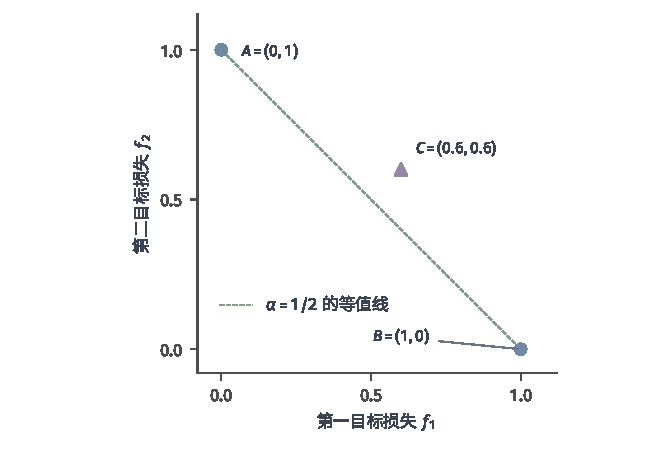
\includegraphics[width=112.0mm]{figures/01-mathematical-preliminaries-upper/01-mathematical-language-combinatorics-analysis-optimization/matplotlib/opt-pareto-weighted-sum/figure.pdf}
  \caption{三个精确可行损失向量，两个目标均需最小化。$A,B,C$互不支配，但对任意$\alpha\in[0,1]$，$C$的加权损失$0.6$都严格大于$\min\{\alpha,1-\alpha\}$。绿虚线仅为$\alpha=1/2$时通过$A,B$的等值线，线上其余点不属于这里的可行集合。因此，Pareto最优不保证能由加权和选到。}
  \label{fig:opt-pareto-weighted-sum}
\end{figure}


在当前点，方向$\bm{d}$若满足
\[
  \langle\nabla f_1(\bm{w}),\bm{d}\rangle<0,\qquad
  \langle\nabla f_2(\bm{w}),\bm{d}\rangle<0,
\]
就是\term{共同下降方向}（common descent direction）。寻找最小范数凸组合
$\alpha\nabla f_1+(1-\alpha)\nabla f_2$相当于把原点投影到两梯度的线段上。

\begin{theorem}[无共同下降方向的一阶判定]
\label{thm:opt-common-descent}
对可微的$m$个目标，在无约束点$\bm{w}$处不存在共同严格下降方向，当且仅当存在
$\alpha_i\geq0$、$\sum_i\alpha_i=1$，使
$\sum_i\alpha_i\nabla f_i(\bm{w})=\bm{0}$。
\end{theorem}

\begin{proof}
若这样的凸组合存在，而$\bm{d}$使每个内积都为负，则加权和内积也为负，与零向量矛盾。
反之，若原点不在梯度集合的凸包中，定理~\ref{thm:opt-projection-separation}给出
$\bm{d}$，使它与每个梯度的内积具有同一严格符号；必要时取$-\bm{d}$，便得到共同严格
下降方向。
\end{proof}

这个条件只排除局部的一阶共同改善，不保证全局Pareto最优；高阶变化或远处方案仍可能
同时改善所有目标。
例如两个目标都为$-x^2$，在$0$的梯度均为零，任意小的非零移动却使两者同时改善。
若目标都凸，零梯度凸组合使相应加权和全局最优，
从而保证弱Pareto最优；要据此得到前面定义的Pareto最优，严格正权重是一条充分条件。
零权重不能省略检查，例如$f_1(x)=0$、$f_2(x)=x^2$在$x=1$满足该一阶判据，
但被$x=0$支配。

共同下降不只是判据，还能给出具体更新。计算权重子问题
\[
 \bm\alpha^\star\in\argmin_{\bm\alpha\in\bm\Delta_m}
 \frac12\left\|\sum_{i=1}^m\alpha_i\nabla f_i(\bm w)\right\|_2^2,
 \qquad
 \bar{\bm g}=\sum_i\alpha_i^\star\nabla f_i(\bm w).
\]
有限梯度的凸包紧且凸，故$\bar{\bm g}$就是原点的唯一投影。
投影最优性给
$\langle\bar{\bm g},\nabla f_i(\bm w)-\bar{\bm g}\rangle\geq0$。
若$\bar{\bm g}\neq0$，取$\bm d=-\bar{\bm g}$便有
$\langle\nabla f_i,\bm d\rangle\leq-\|\bar{\bm g}\|_2^2$对全部$i$成立。
每个目标均$L_i$光滑且$L_i>0$时，任意$0<\eta<2/\max_i L_i$都使
$\bm w^+=\bm w+\eta\bm d$同时降低全部目标；未知常数时，可回溯直至所有目标的
充分下降检验同时通过。若$\bar{\bm g}=0$，算法返回的只是上述一阶证书。
有约束时还要限制$\bm d$的可行性，不能直接使用无约束梯度凸包判据。

例如$f_1(x,y)=((x-1)^2+y^2)/2$、$f_2(x,y)=((x+1)^2+y^2)/2$。
在$(0,1)$两梯度为$(-1,1),(1,1)$，最小范数平均为$(0,1)$；
步长$1$将点移到$(0,0)$，两项目标都由$1$降为$1/2$。
此时梯度为$(-1,0),(1,0)$，原点已在它们之间，不能再共同下降。
加权标量问题的解为$(2\alpha-1,0)$，展示了改变权重怎样沿同一条取舍曲线选择答案。

\paragraph{有限工作点下的预算取舍}
\label{sec:opt-rate-distortion-operating-points}

前沿几何也解释编码中的码率与失真选择。设每个可行方案都有码率$R$和失真$D$，两者越小越好；$R\leq B$下最小化$D$是预算问题，最小化$D+\lambda R$则由$\lambda\geq0$指定取舍。上面的三点反例已经说明：有限方案形成非凸前沿时，某个预算下的最优点仍可能无法由任何加权和选到。只有允许的候选确实包含相应凸组合时，才可以用下凸包代替原可行集合；对编码块或时间作混合，还须计入实际拼接成本。

在光滑、可由支撑线达到的下降曲线$D=D(R)$上，内部最小点满足$D'(R)+\lambda=0$，所以$\lambda$是该处下降斜率的绝对值。若总成本真正可加，且各块的选择互不约束，则$\min\sum_i(D_i+\lambda R_i)$可按块独立选择；总码率预算、上下文依赖或跨块预测可能破坏这种分解。这里建立有限方案的优化关系，概率分布上的率失真函数还需要信息论前提。


\subsection{极小极大优化}
\label{sec:opt-minimax}

多目标问题在同一组变量上比较若干指标；若这些指标分属对立的两方，一方收益就是另一方的
损失，比较关系就从“无法同时改善”变成“同时选择”。
这种结构在机器学习里很常见：生成对抗网络中生成方试图产生难以辨认的样本，判别方则试图区分样本来源。
在鲁棒训练的一个样本$(\bm x,y)$上，固定模型参数$\bm w$后，考虑允许集合$\Delta$
中的特征扰动$\bm\delta$。若$\Delta$非空紧致，且损失$\ell(\bm w,\bm x+\bm\delta,y)$
关于$\bm\delta$连续，内层最大值便能达到，可以选择一个达到它的扰动；
外层再选择$\bm w$，降低这种最坏扰动下的损失。这里改变的是特征，标签$y$保持固定，
允许范围由$\Delta$给出。这样先固定外层选择、再比较全部内层响应，就把“最坏”落实为
指定集合上的最大目标值。用一般变量写，两层的优化方向相反：
\[
  \min_{\bm{w}\in W}\max_{\bm{z}\in Z}\phi(\bm{w},\bm{z}).
\]
外层先选择$\bm w$，内层在看到它后选择使损失最大的$\bm z$。
因此外层实际最小化最坏响应值，不是让两方分别寻找$\phi$的普通最小点。
倒转次序一般会改变值，原始问题返回的是应对最坏响应的决策；
若还返回一对互为最优响应的候选，则需核验下面的鞍点关系。
\begin{definition}[极小极大鞍点]
\label{def:opt-minimax-saddle}
设$W,Z$非空，$\phi:W\times Z\to\mathbb R$。点$(\bm w^\star,\bm z^\star)\in W\times Z$若对所有
$\bm w\in W,\bm z\in Z$满足
\[
  \phi(\bm{w}^{\star},\bm{z})
  \leq\phi(\bm{w}^{\star},\bm{z}^{\star})
  \leq\phi(\bm{w},\bm{z}^{\star})
\]
就称为\term{极小极大鞍点}（minimax saddle point）。
\end{definition}
这里“鞍点”描述两个变量承担
相反优化方向时的全局比较关系，不是第~\ref{sec:multivariable-curvature-error}节中
由单个标量函数的驻点和Hessian矩阵正负曲率定义的微分鞍点。微分鞍点未必求解某个极小
极大问题；极小极大鞍点位于边界或目标不可微时，也未必满足驻点与Hessian判据。
对任意候选对定义
\[
  P(\bm{w})=\sup_{\bm{z}\in Z}\phi(\bm{w},\bm{z}),\qquad
  D(\bm{z})=\inf_{\bm{w}\in W}\phi(\bm{w},\bm{z}).
\]
总有$D(\bm{z})\leq P(\bm{w})$，所以
$P(\bm{w})-D(\bm{z})\geq0$是\term{原始--对偶间隙}
（primal--dual gap）；间隙为零时，该候选对满足鞍点不等式。

本章采用以下有限维极小极大版本：若$W,Z$非空、紧且凸，$\phi$连续，对固定
$\bm{z}$的$\phi(\cdot,\bm{z})$为凸函数，对固定$\bm{w}$的
$\phi(\bm{w},\cdot)$为凹函数，则
\[
  \min_{\bm{w}\in W}\max_{\bm{z}\in Z}\phi(\bm{w},\bm{z})
  =
  \max_{\bm{z}\in Z}\min_{\bm{w}\in W}\phi(\bm{w},\bm{z}),
\]
且两侧最值达到。紧致性提供最值的达到，凸凹性允许用分离比较混合候选，连续性保证极限
不丢失函数值。

可以用前面的分离工具说明交换为何成立。记左侧值为$v$，任取$c<v$。
每个$\bm w\in W$都存在$\bm z$使$\phi(\bm w,\bm z)>c$；
连续性与$W$的紧性给出有限个$\bm z_1,\ldots,\bm z_k$，使每个$\bm w$至少在其中一项超过$c$。
考虑向上封闭的集合
\[
 U=\{\bm a\in\mathbb R^k:\text{存在 }\bm w\in W,\
          \phi(\bm w,\bm z_i)\leq a_i\text{ 对全部 }i\}.
\]
各目标关于$\bm w$凸使$U$凸；$\bm a$的收敛序列所对应的$\bm w$可取收敛子列，
故$U$闭。点$c\bm1$不属于$U$，严格分离给出
$\langle\bm\alpha,c\bm1\rangle<
\inf_{\bm a\in U}\langle\bm\alpha,\bm a\rangle$。
向上封闭迫使$\bm\alpha\geq0$，可归一化为$\sum_i\alpha_i=1$。
于是$\inf_{\bm w}\sum_i\alpha_i\phi(\bm w,\bm z_i)>c$。
令$\bar{\bm z}=\sum_i\alpha_i\bm z_i\in Z$，关于$\bm z$的凹性给
$\phi(\bm w,\bar{\bm z})\geq\sum_i\alpha_i\phi(\bm w,\bm z_i)$，
所以右侧极大极小值大于$c$。令$c\uparrow v$再结合弱对偶，即得值相等。
连续函数在紧积空间上一致连续，使$P,D$分别连续并达到最值；
各取一个达到点就由$D\leq\phi\leq P$得到鞍点。

原始与对偶最优解也可形成这一关系：若零对偶间隙、原始与对偶最优解均达到，
则$\mathcal L(\bm w^\star,\bm y)\leq
\mathcal L(\bm w^\star,\bm y^\star)\leq\mathcal L(\bm w,\bm y^\star)$。
这是Lagrangian的全局鞍点，不是原目标$f$自身的微分鞍点。
鲁棒优化中的$\bm{z}$表示最坏扰动，对抗训练让扰动方提高损失，多任务协调
则可能在权重与模型间形成极小极大结构。若缺少上述条件，两个优化次序可能不同；即使值相等，
具体梯度下降--上升仍可能旋转或发散，值的存在定理不等于算法收敛定理。

取$W=Z=[-1,1]$和$\phi(x,z)=xz$，就能复算这种差别。
$P(x)=|x|$、$D(z)=-|z|$，唯一鞍点为$(0,0)$，候选间隙为$|x|+|z|$。
若两方都作普通最小化，会偏好乘积为$-1$的角点，但在该处最大化方立刻有动机反向行动。
若取同时下降与上升
\[
 x^{(t+1)}=x^{(t)}-\eta z^{(t)},\qquad
 z^{(t+1)}=z^{(t)}+\eta x^{(t)},
\]
暂不投影时有
$(x^{(t+1)})^2+(z^{(t+1)})^2=(1+\eta^2)((x^{(t)})^2+(z^{(t)})^2)$。
每个非零初值都向外旋转。加上盒投影也不保证收敛：
$\eta=1$、初值$(1,0)$时依次得到
$(1,1),(0,1),(-1,1),(-1,0),(-1,-1),(0,-1),(1,-1),(1,0)$，
此后重复，鞍点间隙始终不小于$1$。

一种修正是先试探双方响应，再用试探点的方向更新原点，称为外梯度（extragradient）更新。
记$\bm u=(x,z)^\top$、$\bm F(\bm u)=(z,-x)^\top$、$K=W\times Z$，每轮计算
\[
 \bar{\bm u}^{(t)}=\Pi_K(\bm u^{(t)}-\eta\bm F(\bm u^{(t)})),\qquad
 \bm u^{(t+1)}=\Pi_K(\bm u^{(t)}-\eta\bm F(\bar{\bm u}^{(t)})).
\]
这需要两次方向求值与两次投影。对当前双线性例，在投影未激活时，
更新矩阵为
$\left[\begin{smallmatrix}1-\eta^2&-\eta\\ \eta&1-\eta^2\end{smallmatrix}\right]$，
距离平方每步乘以$1-\eta^2+\eta^4<1$（$0<\eta<1$）。
例如$\eta=1/2$且$\|\bm u^{(0)}\|_2\leq1/2$时，
试探点范数至多$\sqrt{5}/4<1$，后续校正点范数递减，所以所有投影确实都不激活；
此时上述计算完整证明迭代趋于鞍点，间隙也趋零。
这是对该例的可核验改善；一般问题还需梯度映射的单调性和Lipschitz条件等分析，
不能把“多算一次梯度”本身当作收敛定理。


图~\ref{fig:vol1-add-minimax-rotation}对同一双线性目标比较这两种更新。左图追踪候选位置，右图量化到鞍点的距离平方，因而能分清旋转本身与距离是否收缩。
\begin{figure}[!htb]
  \centering
  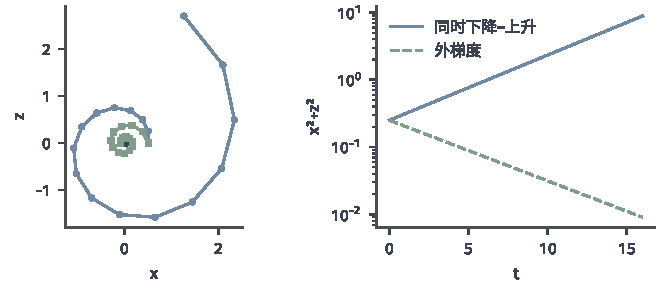
\includegraphics[width=112mm]{figures/01-mathematical-preliminaries-upper/01-mathematical-language-combinatorics-analysis-optimization/matplotlib/comprehension-additions/minimax-rotation.pdf}
  \caption{对$\phi(x,z)=xz$取$\eta=1/2$、初值$(1/2,0)$，展示十六步。蓝线为暂不投影的同时下降--上升，距离平方每步乘$1+\eta^2$；绿线为外梯度，每步乘$1-\eta^2+\eta^4<1$。蓝线离开盒$[-1,1]^2$后只说明无投影更新，不是可行候选；绿线的试探点与校正点始终在盒内，投影未激活。}
  \label{fig:vol1-add-minimax-rotation}
\end{figure}

\subsection{双层优化}
\label{sec:opt-bilevel}

有些决策必须先经过一次学习过程才能评价。例如选择正则强度时，真正决定外层损失的是训练
结束后得到的参数，而不是强度本身；在这个例子中，正则强度先改变内层问题的解，
再由这个解给出评价。超参数调优把模型训练放在内层，把训练后参数的评价放在外层；
元学习也可把任务内适应作为内层过程。前节的鲁棒训练则有不同角色：内层选择使损失
增大的扰动，外层调整模型参数，不是在内层训练模型、外层评价超参数。
这些问题都需说明内层返回什么、外层怎样使用它；把两个目标简单相加，一般不能保留
“必须先满足内层最优性”这一要求。下文以两层都写成最小化的情形建立记号；
内层最大化可通过最小化负目标改写。令外层变量为$\bm\theta\in\Theta\subseteq\mathbb R^p$，
其中$\Theta$是给定的非空允许集合，内层变量取遍$\mathbb R^d$。如果内层问题有
多个最小点，只写
$\bm{w}^{\star}(\bm{\theta})\in
\argmin_{\bm{w}}L_{\mathrm{in}}(\bm{w},\bm{\theta})$
并不能定义一个单值映射，不同最小点还可能给出不同的外层损失。此时可以把最小点集合
上的外层损失下确界、上确界分别定义为乐观、悲观值；只有相应极值达到时，才可写成最小值、最大值。
也可以给定由初始化和算法路径决定的单值选择规则。下文假设内层最小解唯一，或已经给定单值选择$S$，并记
\[
  \bm{w}^{\star}(\bm{\theta})=S(\bm{\theta})
  \in\argmin_{\bm{w}}L_{\mathrm{in}}(\bm{w},\bm{\theta}).
\]
于是外层目标
\begin{equation}
  J(\bm{\theta})
  =L_{\mathrm{out}}(\bm{w}^{\star}(\bm{\theta}),\bm{\theta}).
  \label{eq:opt-bilevel-objective}
\end{equation}
外层要解的是$\min_{\bm\theta\in\Theta}J(\bm\theta)$；上述记号还要求每个允许的$\bm\theta$都有可选的内层最小点。外层不能直接对$\bm\theta$求偏导，因为$J$中的$\bm{w}^\star(\bm\theta)$本身是另一个优化问题的解：没有显式表达式，只能通过内层的驻点条件或迭代过程把对$\bm\theta$的依赖传到外层。下面两条路线正对应这两种做法。
这种把另一优化问题的解作为评价输入的问题称为\term{双层优化}（bilevel optimization）。元学习把内层看成任务适应，超参数
选择让$\bm{\theta}$控制正则强度或数据权重，定向知识修正则让外层评价修改后的特定行为。
例如$L_{\mathrm{in}}(w,\theta)=(w^2-1)^2$的最小点始终为$\{-1,1\}$，
外层取$L_{\mathrm{out}}(w,\theta)=(w-\theta)^2/2$。
在$\theta=1$，乐观选解的外层值为$0$，悲观选解的值为$2$。
内层最优值相同并不使外层值相同；选择规则还可能随$\theta$发生切换。

一种求导方式是把$T$步内层更新全部展开。例如
$\bm{w}^{(t+1)}=\bm{w}^{(t)}-\eta\nabla_{\bm{w}}
L_{\mathrm{in}}(\bm{w}^{(t)},\bm{\theta})$，再按链式法则从$t=T$反向传播。
展开法忠实求导于“运行$T$步”这个实际算法，但存储随$T$增长，且所得梯度对应近似内层解，
不一定对应精确最优解。

两步展开已经能看清链式结构。设$\bm w\in\mathbb R^d$、$\bm\theta\in\mathbb R^p$，
并设$L_{\mathrm{in}}$二阶连续可微，固定不依赖$\bm\theta$的步长$\eta$，记$d\times d$和$d\times p$矩阵分别为
\[
  \bm{A}^{(t)}=\bm{I}-\eta\nabla_{\bm{w},\bm{w}}^2
  L_{\mathrm{in}}(\bm{w}^{(t)},\bm{\theta}),\qquad
  \bm{B}^{(t)}=\nabla_{\bm{w},\bm{\theta}}^2
  L_{\mathrm{in}}(\bm{w}^{(t)},\bm{\theta}).
\]
则
\[
  \frac{d\bm{w}^{(t+1)}}{d\bm{\theta}}
  =\bm{A}^{(t)}\frac{d\bm{w}^{(t)}}{d\bm{\theta}}-\eta\bm{B}^{(t)},
\]
从而
\[
  \frac{d\bm{w}^{(2)}}{d\bm{\theta}}
  =\bm{A}^{(1)}\bm{A}^{(0)}\frac{d\bm{w}^{(0)}}{d\bm{\theta}}
  -\eta\bm{A}^{(1)}\bm{B}^{(0)}-\eta\bm{B}^{(1)}.
\]
记有限步外层目标为$J_T(\bm\theta)=L_{\mathrm{out}}(\bm w^{(T)}(\bm\theta),\bm\theta)$。
由于$\bm D_T=d\bm w^{(T)}/d\bm\theta$是$d\times p$矩阵，列梯度的链式法则为
\[
 \nabla_{\bm\theta}J_T
 =\bm D_T^\top\nabla_{\bm w}L_{\mathrm{out}}
  +\nabla_{\bm\theta}L_{\mathrm{out}},
\]
右侧两项都在$(\bm w^{(T)},\bm\theta)$计算，第二项固定$\bm w$求偏导；转置后两项都是$p$维列向量。
减少前向更新步数会改变$J_T$。若仍运行相同的$T$步，只截断反向导数传播，
前向目标不变，但Jacobian中的部分乘积项被舍去，通常得到同一$J_T$的近似梯度。
若步长或初始化本身依赖外层参数，其导数也必须保留；
若更新含不可微投影或离散分支，普通链式法则需要另外检查分支与可微条件。

取$L_{\mathrm{in}}(w,\theta)=(w-\theta)^2/2$、$w^{(0)}=0$与$\eta=1/2$。
两步得到$w^{(1)}=\theta/2$、$w^{(2)}=3\theta/4$，对应导数为$1/2,3/4$。
本例另取外层损失$(w-1)^2/2$，它不直接依赖$\theta$。在$\theta=2$有$w^{(2)}=3/2$，
两步外层梯度为$(3/2-1)(3/4)=3/8$；
理想内层解$w^\star=\theta$对应梯度却为$\theta-1=1$。
两者都算得正确，求导的对象不同。在这个例子中，
$w^{(T)}=(1-2^{-T})\theta$及其导数都趋向理想分支；一般问题需要额外控制
迭代收敛与导数乘积，不能由有限步求导自动得到这个极限。图~\ref{fig:opt-bilevel-target-chains}将这两个不同目标的计算链并列。

\begin{figure*}[htbp]
  \centering
  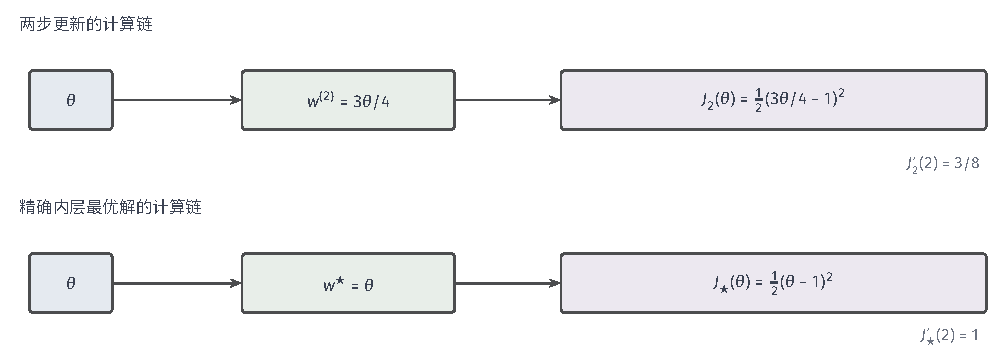
\includegraphics[width=168.998mm]{figures/01-mathematical-preliminaries-upper/01-mathematical-language-combinatorics-analysis-optimization/tikz/opt-bilevel-target-chains/figure.pdf}
  \caption{同一二次内层目标的两条计算链。固定$w^{(0)}=0$、步长$1/2$，两次更新产生$w^{(2)}=3\theta/4$；精确最优解则为$w^\star=\theta$。外层都读取$(w-1)^2/2$，但两个复合目标不同，故在$\theta=2$处分别得到导数$3/8$与$1$。有限步算法的求导与精确解分支的求导各自对应自己的目标。}
  \label{fig:opt-bilevel-target-chains}
\end{figure*}



隐式求导跟踪的是一个选定的非退化局部最小点分支，不自动证明该分支实现全局最小值。
只有当这个分支也是全局最小点并符合前述选择规则时，它才与
$\bm{w}^{\star}(\bm{\theta})$及$J$对应。为区分两者，记局部分支及其外层目标为
$\widehat{\bm{w}}(\bm{\theta})$和
$\widehat{J}(\bm{\theta})
=L_{\mathrm{out}}(\widehat{\bm{w}}(\bm{\theta}),\bm{\theta})$。
若$L_{\mathrm{in}}$二阶连续可微，并且
\[
  \nabla_{\bm{w}}L_{\mathrm{in}}
  (\widehat{\bm{w}}(\bm{\theta}),\bm{\theta})=\bm{0},
\]
记在该分支上计算的二阶导数为
$\bm{H}_{w,w}=\nabla_{\bm{w},\bm{w}}^2L_{\mathrm{in}}$和
$\bm{H}_{w,\theta}=\nabla_{\bm{w},\bm{\theta}}^2L_{\mathrm{in}}$。
对驻点方程关于$\bm{\theta}$求导得到
\[
  \bm{H}_{w,w}\frac{d\widehat{\bm{w}}}{d\bm{\theta}}
  +\bm{H}_{w,\theta}=\bm{0}.
\]
当$\bm{H}_{w,w}$可逆时，第~\ref{chap:multivariate-calculus}章的隐函数定理给出局部可微分支；
固定参数时，这个驻点在附近是孤立的。对非退化局部最小点，
$\bm{H}_{w,w}\succ\bm{0}$保证这一可逆性。链式法则于是给出
\begin{equation}
  \nabla_{\bm{\theta}}\widehat{J}
  =
  \nabla_{\bm{\theta}}L_{\mathrm{out}}
  -\bm{H}_{w,\theta}^{\top}
  \bm{H}_{w,w}^{-\top}
  \nabla_{\bm{w}}L_{\mathrm{out}}.
  \label{eq:opt-implicit-hypergradient}
\end{equation}
式~\eqref{eq:opt-implicit-hypergradient}是\term{隐式超梯度}
（implicit hypergradient）。实际计算通常解线性方程
$\bm{H}_{w,w}^{\top}\bm{v}=\nabla_{\bm{w}}L_{\mathrm{out}}$，无须显式求逆。

用二次内层目标可以核对公式。设$\bm H\in\mathbb R^{d\times d}$对称正定，$\bm B\in\mathbb R^{d\times p}$、$\bm C\in\mathbb R^{m\times d}$、$\bm d\in\mathbb R^m$，
\[
  L_{\mathrm{in}}(\bm{w},\bm{\theta})
  =\frac12(\bm{w}-\bm{B}\bm{\theta})^{\top}
  \bm{H}(\bm{w}-\bm{B}\bm{\theta}),\qquad
  L_{\mathrm{out}}(\bm{w})
  =\frac12\lVert\bm{C}\bm{w}-\bm{d}\rVert_2^2.
\]
这里内层最小点唯一，因此局部分支与全局选择一致：
$\widehat{\bm{w}}=\bm{w}^{\star}=\bm{B}\bm{\theta}$且
$\widehat{J}=J$。直接消元给出
\[
  \nabla_{\bm{\theta}}J
  =\bm{B}^{\top}\bm{C}^{\top}
  (\bm{C}\bm{B}\bm{\theta}-\bm{d}).
\]
隐式公式中$\bm{H}_{w,w}=\bm{H}$、
$\bm{H}_{w,\theta}=-\bm{H}\bm{B}$，代入后得到同一结果。计算时若线性方程残差为
$\bm r=\bm H^\top\widetilde{\bm v}-\nabla_{\bm w}L_{\mathrm{out}}$，
解误差为$\widetilde{\bm v}-\bm v=\bm{H}^{-\top}\bm{r}$；小特征值会放大该误差。因而内层驻点残差、
线性求解残差和曲率病态是三种不同的误差来源。

若内层只近似收敛，驻点残差会进入超梯度误差；若Hessian矩阵奇异，解映射可能不唯一或不可微；
若内层非凸，所选局部分支还依赖初始化与算法路径，并且可能不是全局最小点。后一种情况下，
式~\eqref{eq:opt-implicit-hypergradient}给出的是$\widehat{J}$的梯度，而不是前述全局
双层目标$J$的梯度。展开深度、线性方程精度、内层计算预算与解选择规则因此都是问题定义的
一部分，而不只是实现细节。

误差可在局部强凸条件下定量分开。固定$\bm\theta$，设近似点$\widetilde{\bm w}$
与选定分支$\widehat{\bm w}$之间的凸邻域满足
$\nabla_{\bm w,\bm w}^2L_{\mathrm{in}}\succeq\mu\bm I$，$\mu>0$。
内层残差$\bm r_{\mathrm{in}}=\nabla_{\bm w}L_{\mathrm{in}}(\widetilde{\bm w},\bm\theta)$满足
\[
 \|\widetilde{\bm w}-\widehat{\bm w}\|_2
 \leq\frac{\|\bm r_{\mathrm{in}}\|_2}{\mu},
\]
因为梯度沿线段积分后，与位移的内积至少为$\mu$倍距离平方。
在近似点计算内层Hessian$\widetilde{\bm H}$、混合导数
$\widetilde{\bm B}=\nabla_{\bm w,\bm\theta}^2L_{\mathrm{in}}(\widetilde{\bm w},\bm\theta)$
及外层梯度，再近似求解伴随方程，
令$\bm r_{\mathrm{lin}}=\widetilde{\bm H}^{\top}\widetilde{\bm v}
-\nabla_{\bm w}L_{\mathrm{out}}(\widetilde{\bm w},\bm\theta)$。
线性求解单独贡献的超梯度误差至多为
$\|\widetilde{\bm B}\|_2\|\bm r_{\mathrm{lin}}\|_2/\mu$。
若这些一、二阶导数在该邻域有界且Lipschitz，精确线性求解所定义的超梯度表达式
作为$\bm w$的函数有某个有限Lipschitz常数$C$。记由近似点与近似伴随解算出的
超梯度为$\widetilde{\nabla_{\bm\theta}\widehat J}$，则总误差满足
\begin{equation}
 \|\widetilde{\nabla_{\bm\theta}\widehat J}-\nabla_{\bm\theta}\widehat J\|_2
 \leq\frac C\mu\|\bm r_{\mathrm{in}}\|_2
 +\frac{\|\widetilde{\bm B}\|_2}{\mu}\|\bm r_{\mathrm{lin}}\|_2.
 \label{eq:opt-hypergradient-two-residuals}
\end{equation}
右侧第一项来自内层点不够准确，第二项来自同一点上的线性系统未解准。
只压低其中一项不足以控制总误差，小$\mu$也会同时放大二者。
取得外层方向后，可再对选定的外层目标执行梯度或投影更新；
只有所求超梯度对应的目标和误差范围明确，才能复用前面带误差更新的分析。

\section{本章小结}
\label{sec:opt-summary}

最优化需要分别回答四个问题：候选解是否存在，某个点为何最优，算法怎样到达它，以及误差
按什么尺度收敛。连续性配合紧致性保证存在；在闭域上，下半连续性与强制性也能通过紧
下水平集保证存在。凸性把局部条件提升为全局条件，强凸、光滑性与PL条件则分别控制参数
距离、单步上界和目标误差。它们不能只用“曲率好”一语合并。

共同二次目标$(w_1^2+16w_2^2)/2$展示了这些条件怎样进入计算：
统一梯度步受曲率$16$限制，动量改变历史响应，预条件调整两个方向的尺度，
牛顿法则直接解曲率方程。它们对同一个无约束答案付出不同的信息与计算成本。
加上$\ell_1$项后，软阈值使尖点可精确处理；加上$w_1+w_2=1$后，
二次惩罚的有限参数解仍不满足等式，乘子平衡才给出约束解$(16/17,1/17)$。
因此比较方法要固定原任务、返回质量及成本口径，不能只看更新式是否更复杂或步数是否更少。

带资源约束后，KKT条件描述目标梯度与约束法向量的平衡，对偶变量提供界和敏感性解释。
Farkas证书与线性规划强对偶说明最优值相等需要证明，不能从凸性直接跳得。松弛、对偶界与
可行解共同形成最优性证书；乘子更新提供寻找下界的过程，原解恢复仍需单独保证可行性。
预算例中，对偶值持续改善时原始副本仍可能违规，这正是不能把求解过程与证书混为一谈的原因。

非线性残差中，LM调节本轮位移并核验真实下降；IRLS通过同一残差代价的切线上界重新分配权重；STE则另外指定离散运算的反向规则。只有前两者在相应接受或代理改善条件下保留目标下降，第三者需要单独检查前向损失。有限码率与失真选择也必须回到实际可行工作点，不能把加权和的支撑点当作全部预算最优解。

\begin{samepage}
计算预算不足时，可以组合代理、分块及近似更新，但必须分别记录误差来源及其累计方式。
目标下降中的平方误差和，与轨迹偏差中的一次范数和，控制不同对象；
副本一致、块最优和联合最优也需要不同条件。多个指标进一步要求约定权重或Pareto比较，
竞争要求核验最坏响应及鞍点间隙，嵌套要求区分有限步输出、局部驻点分支与理想全局内层解。
这些答案都可以“足够好”，但必须说明好在哪个尺度、满足哪些约束、花了多少计算。
随机逼近还需要条件期望、噪声与平均动力学工具，策略评价则会复用本章的对偶与鞍点语言。
第~\ref{chap:functional-analysis-and-approximation}章将把有限维参数推广到函数空间，
区分表示存在性、逼近误差与函数类复杂度。

\end{samepage}

